
      \pagestyle{headings}

	% \part{Description of software contents}{Description of software contents}

                                  \section*{PREFACE TO THE BNL EDITION, 2012} 
\addcontentsline{toc}{section}{\numberline{}PREFACE TO THE BNL EDITION (2012)} 

The previous release of the Zgoubi Users' Guide as a Lab. report dates from 1997, making the present one  the 
latest in a series of~five~\cite{Biblio1}-\cite{Biblio2c}. 

\bigskip

\noindent \zgoubi\ has undergone substantial developments since the 
4th edition of the Users' Guide,  in the frame of a number of 
projects and of beam dynamics studies, as the Neutrino Factory, lepton and hadron colliders, 
spin dynamics investigations at SuperB, RHIC, etc. 
As well  the list of optical elements has grown, 
and so did the  ``Glossary of Keywords'' list, pp.~\pageref{GOK1A} and~\pageref{GOK1B}, including  new 
simulation and computing procedures, which range from constraint-matching to overlapping magnetic fields capabilities to 
spin manipulations  and other synchrotron radiation damping recipes. 


\bigskip

\noindent The code has been installed on SourceForge with the collaboration of J.~S.~Berg, in Sept.~2007, 
there it is fully and freely available~\cite{SFZ}. The SourceForge package evolves and is maintained at the 
pace of on-going projects and design studies.   It includes the source files, 
the post-processor program \zpop, as well as many examples with their  input 
data files (``zgoubi.dat'') and  output result files (``zgoubi.res''). 


\bigskip

\noindent A series of auxiliary computing tools have been developed in addition, 
 aimed at making the designer's life easier, as, 
 search for closed orbits\index{closed orbit}  in periodic machines, computation of optical functions and parameters, 
tune scans, dynamic aperture scans,   spin dynamics data treatment, 
 graphic scripts, etc., and including dedicated ones regarding, \emph{e.g.}, FFAG and cyclotron design, 
AGS and RHIC studies, synchrotron radiation losses and their effects. 
In addition ``python'' interfaces are being developed by several users,  possibly made available on web 
by their authors. 

\bigskip

\noindent  The Users' Guide is intended  to describe the contents of the most
recent version of \zgou. The code and its Guide are  both far from being  ``finished products''. 

\bigskip

\noindent J.~S.~Berg and N.~Tsoupas, BNL, have reviewed the final proof of the present document. 


\newpage
\clearemptydoublepage

                                  \section*{INTRODUCTION TO THE 4th  EDITION, 1997}
\addcontentsline{toc}{section}{\numberline{}INTRODUCTION TO THE 4th  EDITION (1997)}

The initial  version of \zgoubi, dedicated to  ray-tracing in magnetic fields,
 was developed  by D.~Garreta and J.C.~Faivre  at CEN-Saclay in the early 1970's.
 It was perfected for the purpose of studying the four spectrometers SPES I, II, III, IV  
at the  Laboratoire National SATURNE (CEA-Saclay, France), and SPEG at GANIL 
(Caen, France). It is being used since long in several national and foreign laboratories.
\\
\\
\noindent The first manual was in French~\cite{Biblio1}. %%%%biblio  [1]
 Accounting for  many developments and improvements, and in order to facilitate access to 
the program an English version of the manual was written at TRIUMF with the assistance of 
J.~Doornbos. P.~Stewart prepared the manuscript for publication~\cite{Biblio2}%biblio[2].
\\
\\
\noindent  An updating of the latter was necessary for accompanying the third version of the code which included 
 developments regarding  spin tracking and ray-tracing in combined electric and magnetic fields~; 
 this was done with the help of 
D.~Bunel (SATURNE Laboratory, Saclay) for the preparation of the document and lead to the third 
release~\cite{Biblio2b}.
\\
\\
\noindent In the mid-1990s,  the computation of synchrotron radiation electromagnetic impulse and spectra 
was introduced for the purpose of studying interference effects at the LEP 
synchrotron radiation  based diagnostic mini-wiggler. In the mean 
time, several new optical elements were added, such as 
electro-magnetic and other electrostatic lenses. Used since several years for special studies in periodic
machines (\emph{e.g.}, SATURNE at Saclay, COSY at Julich, LEP and LHC at CERN, Neutrino Factory rings),  
\zgou\  has also undergone extensive developments regarding storage ring related features.
\\
\\
\noindent These  developments of \zgou\ 
 have strongly benefited of the environment of the Groupe Th\'eorie, 
Laboratoire National SATURNE, CEA/DSM-Saclay, in the years 1985-1995. 
\\
\\
The graphic  interface to \zgou\ (addressed in Part D) has also undergone concomitant extensive  
developments, which make it a performing tool for the post-processing of \zgou\  outputs.
\\
\\
\noindent  The Users' Guide is intended  to describe the contents of the most
recent version of \zgou, which is far from being a ``finished product''.




\newpage
\clearemptydoublepage

\section*{INTRODUCTION} 
\addcontentsline{toc}{section}{\numberline{}INTRODUCTION}

The computer code \zgou\  calculates trajectories of
charged particles in magnetic and electric fields.  At the origin specially adapted to the definition and adjustment of 
beam lines and magnetic spectrometers, it has so evolved that it allows the study of systems including complex
 sequences of optical elements such as dipoles, quadrupoles, 
 arbitrary multipoles, FFAG magnets and other magnetic or electric
 devices, and is able as well to handle periodic structures.  Compared to other codes, 
it presents several peculiarities, as follows - a non-exhaustive list~: 
\begin{itemize}
\item a numerical method for integrating the Lorentz equation, based on Taylor series,
	which optimizes computing time and provides high accuracy and strong symplecticity,
\item spin tracking, using the same numerical method as for the Lorentz equation,
\item account of stochastic photon emission, and its effects on particle dynamics, 
\item calculation of the synchrotron radiation electric field and 
spectra in arbitrary magnetic fields, from the ray-tracing outcomes,
\item the possibility of using a mesh, which allows ray-tracing from
	simulated or measured (1-D, 2-D or 3-D) electric and magnetic field maps, 
\item a number  Monte Carlo procedures~: unlimited number of trajectories, in-flight decay, 
stochastic radiation, etc., 
\item built-in fitting procedures allowing arbitrary variables and a large variety of 
constraints, easily expandable, 
\item multi-turn tracking in circular accelerators including  features proper to machine 
parameter calculation and survey,  
\item simulation of time-varying power  supplies, 
\item simulation of arbitrary radio-frequency programs.
\end{itemize}

\medskip

\noindent The initial  version of \zgoubi\ was dedicated to  ray-tracing in magnetic elements, beam lines, spectrometers. 
 It was perfected for the purpose of studying, and operating, the four spectrometers SPES I, II, III, IV  
at the  Laboratoire National SATURNE (CEA-Saclay, France), and, later,  SPEG at GANIL 
(Caen, France). 

\medskip

\noindent Developments regarding  spin tracking and ray-tracing in combined electric and magnetic fields
were implemented, in the late 1980s and early 1990s respectively.  

\medskip

\noindent In the mid-1990s,  the computation of 
synchrotron radiation electromagnetic impulse and spectra was introduced, 
for the purpose of synchrotron radiation diagnostic R\&D at LEP, and further applied to the 
design of the SR diagnostics installations at LHC in the early 2000s. 
In the mean time, several new optical elements were added, such as 
electro-magnetic and other electrostatic lenses. Used since several years for special studies in periodic
machines (\emph{e.g.}, SATURNE at Saclay, COSY at Julich, LEP and LHC at CERN),  
\zgou\  has also undergone extensive developments regarding storage ring related features.

\medskip

\noindent Many developments have been accomplished since the early 2000s in the frame of a number of 
project design and beam dynamics studies, as the neutrino factory, lepton and hadron colliders, 
spin studies at AGS and RHIC, etc. 
As a consequence the list of optical elements and the compendium of numerical methods, 
so-called ``Glossary of Keywords'' list, pp.~\pageref{GOK1A} and~\pageref{GOK1B},
  has stretched with new 
simulation and computing procedures, ranging from fitting (\textsl{FIT2} procedure~;  
additional constraints) to overlapping magnetic field  capabilities (\textsl{DIPOLES}, \textsl{FFAG}), 
spin manipulation (\textsl{SPINR}), optical elements (\textsl{BEAMBEAM}),  radiation damping tools (\textsl{SRLOSS}) 
and many others (\textsl{FAISTORE}, \textsl{MAP2D-E}, \textsl{OPTICS}, \textsl{PICKUPS}, \textsl{TWISS}, etc.). 

\medskip

\noindent The graphic  interface to \zgou\ (\zpop, Part~D) has undergone  extensive  developments, making it 
a convenient companion tool to the use of \zgoubi. 




\newpage
\clearemptydoublepage

\section{NUMERICAL CALCULATION OF MOTION AND FIELDS}\label{sec2} %%2


\subsection{\zgoubi\ Frame} \label{sec2.1}   %%2.1

The reference frame of \zgou\  is presented in Fig.~\ref{fig1}.  
Its origin is in the median plane on a reference curve which generally (but not always) coincides with the optical 
axis of optical elements. 

\subsection{Integration of the Lorentz Equation} \label{sec2.2}%%%2.2

The Lorentz equation, which governs the motion of a particle of charge $q$,  relativistic 
mass $m$ and velocity $\vec  v$ in electric and magnetic fields $\vec  e$ and $\vec  b$, is written 
%
\begin{equation}
\dfrac{d(m\vec  v)}{dt} = q\, (\vec  e + \vec  v \times  \vec  b)  \label{eq2-2-1}
\end{equation}
%
\noindent Noting $()' = \dfrac{d()}{ds} $ ~  and taking      
%
\begin{equation}
\vec  u = \dfrac{\vec  v }{v},\quad
    	ds = v\,dt \ ,\quad
		\vec  u^{\,\prime}  =\dfrac{d\vec  u }{ds} \ ,\quad
			 m\vec  v = mv\vec  u = q\, \Br \, \vec  u \label{eq2-2-2}
\end{equation}
 where $ \Br $ is the rigidity of the particle, this equation can be rewritten 
%
\begin{equation}
(\Br )^\prime \, \vec  u +\Br \,\vec  u^{\,\prime}  
	=  \dfrac{\vec  e }{v}  + \vec  u  \times   \vec  b   \label{eq2-2-3}
\end{equation}
%
\noindent From position $ \vec  R(M_0) $ and unit velocity $ \vec  u(M_0) $ at
point $ M_0 $, position $ \vec  R(M_1) $ and unit velocity $ \vec  u(M_1) $ 
at point $ M_1 $ following a 
displacement  $ \Delta s $, are obtained from truncated Taylor expansions (Fig.~\ref{fig2})  
%
\begin{equation}
\begin{aligned}
\vec  R(M_1)  &  \approx  \vec  R(M_0) + \vec  u(M_0)\, \Delta s+ \vec  u^{\,\prime} (M_0)\,
	\dfrac{\Delta s^2 }{2!}  +  ...+ \vec  u^{\cinqprime} (M_0)\,
	\dfrac{\Delta s^6 }{6!} \\
\vec  u(M_1) & \approx  \vec u(M_0)  + \vec  u^{\,\prime} (M_0)\,\Delta s  + \vec  u^{\,\prime\prime} (M_0)\,
	\dfrac{\Delta s^2 }{2!}  +   ...+ \vec  u^{\cinqprime} (M_0)\,
	\dfrac{\Delta s^5 }{5!} 
\end{aligned}\label{eq2-2-4}
\end{equation}
%
\noindent The rigidity at $ M_1 $ is obtained in the same way from
\begin{equation}
 (\Br )(M_1) \approx (\Br )(M_0)+(\Br )^\prime (M_0)\Delta s+...+
	(\Br)^{\quaprime\prime} (M_0) \dfrac{\Delta s^5 }{5!}   	\label{eq2-2-5}
\end{equation}
%
\noindent The equation of time of flight is written in a similar manner 
\begin{equation}
 T(M_1) \approx   T(M_0) +  T' (M_0)\, \Delta s+ T'' (M_0)\,\dfrac{\Delta s^2}{2} + 
    ~ ... ~  + T^{\quaprime\prime} (M_0)\,\dfrac{\Delta s^5}{5!} 	\label{eq2-2-Time}
\end{equation}


\noindent The derivatives $\vec  u^{(n)} = \dfrac{d^n\vec  u}{ds^n}$ and 
$ (\Br )^{(n)} = \dfrac{d^n(\Br )}{ds^n} $
involved in these expressions are calculated as described in the next sections. 
For the sake of computing speed, three distinct software procedures are involved, depending on 
whether $\vec e$ or $\vec  b$ is zero, or $ \vec e$ and $ \vec b$ are 
both non-zero.

%%%%%%%%%%%%%%figure%%%%%%%%%%%%%%
\vspace{0cm}
\begin{figure}[H]
%\vspace{11 truecm}
%%%Figure 1
\centerline{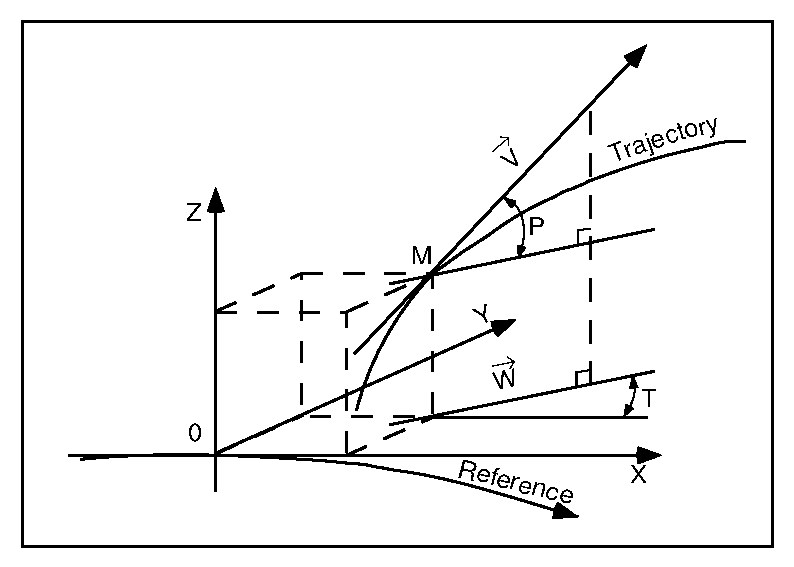
\includegraphics[width=14cm]{Fig1.ps}}
\hangcaption[Fig 1]{\label{fig1}Reference frame and coordinates ($Y$, 
$T$, $Z$, $P$) in \zgou.\\
$ OX$~:   in the direction of motion,\\
$ OY$~:   normal to $OX$,\\
$ OZ$~:  orthogonal to the $(X, Y)$ plane,\\				  
$ \vec{W}$~:  projection of the velocity, $ \vec	v $, in	the	$(X, Y)$ plane,\\									  %
$ T$  =	 angle between $\vec{W}$ and the  $X$-axis,\\
$ P$  =	 angle between $\vec{W}$ and $	\vec  v	$. } 
%\end{figure}
\vspace{.3cm}
%%%%%%%%%%%%%%%%%%%%figure%%%%%%%%%%%%%%%%%%%%%
%\begin{figure}[H]
%\vspace{10 truecm}
%%%Figure 2~: 
\centerline{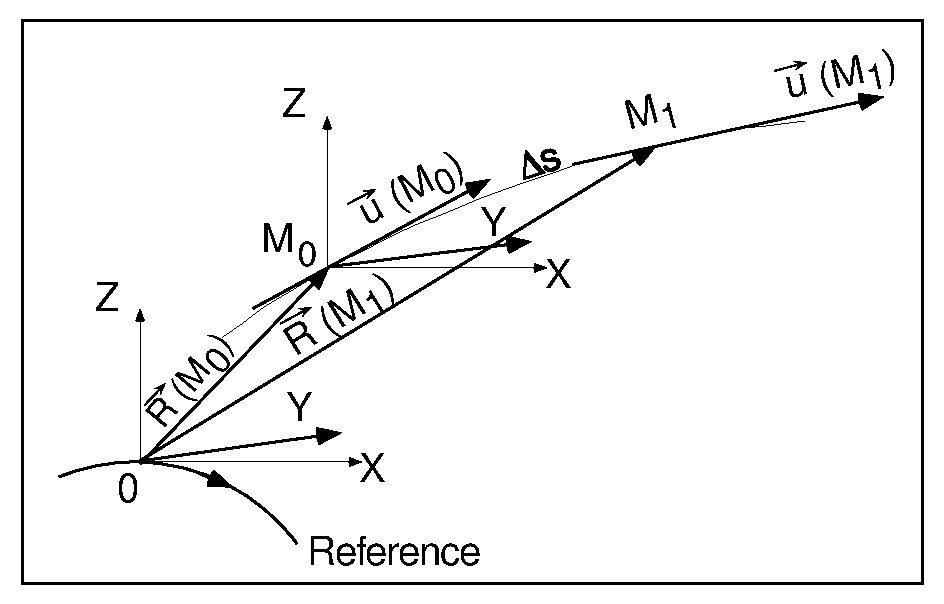
\includegraphics[width=14cm]{Fig2.ps}}
\hangcaption{\label{fig2} Position and velocity of a particle in the reference frame.}
\end{figure}

\subsubsection{Integration in Magnetic Fields} \label{sec2.2.1}  %% 2.2.1.

Considering  $ \vec  e=0 $ and given  $ \vec B=\dfrac{\vec  b}{\Br} $, 
eq.~(\ref{eq2-2-3}) reduces to 
\begin{equation}
 \vec  u^{\,\prime}  = \vec  u  \times  \vec  B   	\label{eqBBrho}
\end{equation}

\noindent The successive derivatives $\vec  u^{(n)} = \dfrac{d^n\vec  u }{ds^n} $ of 
$ \vec  u $ needed in the Taylor expansions (eqs.~\ref{eq2-2-4}) are calculated by differentiating 
$ \vec  u^{\,\prime}            =\vec  u  \times  \vec  B$ 

\begin{equation}
	\begin{aligned}
		\vec  u^{\,\prime\prime}
		         &   =   \vec  u^{\,\prime}   \times   \vec  B + \vec  u  \times  
		         \vec B^{\,\prime} \\
		\vec u^{\,\prime\prime\prime}
		         & = \vec  u^{\,\prime\prime}   \times   \vec  B 
		         + 2\vec  u^{\,\prime}  \times   \vec  B^{\,\prime}  
		         + \vec  u \times  \vec  B^{\,\prime\prime} \\
		\vec u^{\quaprime} 
		         &   =  \vec u^{\,\prime\prime\prime}  \times   \vec  B 
		         + 3\vec  u^{\,\prime\prime}   \times  \vec  B^{\,\prime}  
		         + 3\vec  u^{\,\prime}   \times   \vec  B^{\,\prime\prime}   
		         +\vec	u  \times  \vec  B^{\,\prime\prime\prime} \\
		\vec  u^{\cinqprime}
		         &  =  \vec u^{\quaprime}  \times \vec  B 
		         + 4\vec u^{\,\prime\prime\prime}  \times  \vec  B^{\,\prime}  
		         + 6\vec  u^{\,\prime\prime} \times   \vec  B^{\,\prime\prime}  
		         + 4\vec  u^{\,\prime}   \times   \vec B^{\,\prime\prime\prime} 
		         + \vec  u  \times   \vec  B^{\quaprime}
	\end{aligned}
	\label{eq2-2-6}
\end{equation}
%
 where $ \vec  B^{(n)} = \dfrac{d^n\vec  B}{ds^n}$. 

\noindent From  
\begin{equation} d\vec  B = \dfrac{\partial\vec  B}{\partial X}\, dX
     +\dfrac{\partial\vec  B}{\partial Y}\, dY+
     \dfrac{\partial\vec  B}{\partial Z}\, dZ
     = \sum_{i=1,3}\dfrac{\partial\vec  B}{\partial X_i}\, dX_i
 	\label{eq2-2-7a}
\end{equation}
and by successive differentiation, we get 

 \begin{equation}
	 \begin{aligned}
		 \vec  B^{\,\prime} =
		        &   \sum_i  \dfrac{\partial\vec  B}{\partial X_i}\, u_i \\
		 \vec  B^{\,\prime\prime} =
		        &  \sum_{ij}\dfrac{\partial^2\vec  B}{\partial X_i\partial X_j} 
		        \, u_i u_j+ \sum_i \dfrac{\partial\vec  B}{\partial X_i} \,u^{\,\prime}_i\\
		\vec  B^{\,\prime\prime\prime}  =
		        &  \sum_{ijk} \dfrac{\partial^3\vec  B}{\partial X_i\partial X_j\partial X_k}
		           \, u_i u_j u_k 
		           + 3 \sum_{ij} \dfrac{\partial^ 2\vec  B}{\partial X_i\partial X_j} \,u^{\prime}_i
		           u_j 
		           + \sum_i\dfrac{\partial\vec  B}{\partial X_i} \, u^{\prime\prime}_i \\
		\vec B^{\quaprime}  = 
		        & \sum_{ijkl} \dfrac{\partial^ 4\vec  B}{\partial X_i\partial X_j\partial
		           X_k\partial X_l} \,u_i u_j u_k u_l 
		           + 6 \sum_{ijk}  \dfrac{\partial^ 3\vec  B}{\partial X_i\partial X_j\partial X_k} \,
		           u^{\prime}_i u_j u_k \\
		        &
		        +  4 \sum_{ij} \dfrac{\partial^ 2\vec  B}{\partial X_i\partial X_j}\,
		         u^{\prime\prime}_i u_j
		         + 3 \sum_{ij} \dfrac{\partial^ 2\vec  B}{\partial X_i\partial X_j}\,
		         u^{\prime}_i u^{\prime}_j 
		         + \sum_i \dfrac{\partial\vec  B}{\partial X_i}\, u^{\prime\prime \prime}_i 
	 \end{aligned}
 	\label{eq2-2-7}
 \end{equation} 
 %
 \noindent From the knowledge of $ \vec  u(M_0) $ and $ \vec  B(M_0) $ at point
$ M_0 $ of the 
trajectory, we calculate alternately the derivatives of $ \vec  u(M_0) $ and 
$ \vec  B(M_0) $, by means of eqs.~(\ref{eq2-2-6}) and (\ref{eq2-2-7}), and inject these into eq.~(\ref{eq2-2-4}) 
 so yielding $ \vec  R(M_1) $ and $ \vec  u(M_1) $.


\subsubsection[Integration in Electric Fields]%
       {Integration in Electric Fields~\protect\cite{Biblio6}}
        \label{sec2.2.2} %%%% 2.2.2.[3]

Admitting that $ \vec  b=0, $ eq.~(\ref{eq2-2-3}) reduces to 

\begin{equation}
	(\Br )^\prime\vec  u + \Br\vec  u^{\,\prime} = \dfrac{\vec  e}{ v}
	\label{eq2-2-8}
\end{equation} 
%
which, by successive differentiations, gives the recursive relations

\begin{equation}
	\begin{array}{l}
		(\Br )^\prime\vec  u + \Br\vec  u^{\,\prime}   = \dfrac{\vec e}{ v}\\
		 (\Br )^{\prime\prime}\vec  u + 2 (\Br)^\prime \vec  u^{\,\prime} 
		     +\Br\vec  u^{\,\prime\prime}   = \left(\dfrac{1}{v}\right)^\prime\vec  e 
		         + \dfrac{\vec  e^{\,\prime}}{v} \\
		(\Br)^{\prime\prime\prime}\vec  u + 3(\Br)^{\prime\prime}\vec  u^{\,\prime}
		      + 3(\Br)^\prime \vec  u^{\,\prime\prime} 
		      +\Br\vec  u^{\prime\prime\prime}   =
		      \left(\dfrac{1}{ v}\right)^{\prime\prime}\vec  e +
		      2\left( \dfrac{1}{v}\right)^\prime \vec  e^{\,\prime} 
		      +\left(\dfrac{1}{v}\right)\, \vec  e^{\,\prime\prime}\\
		(\Br )^{\quaprime} \vec u + 4(\Br)^{\prime\prime\prime} \vec  u^{\,\prime} 
		      + 6(\Br)^{\prime\prime}\vec  u^{\,\prime\prime} 
		      +4 (\Br)^\prime\vec  u^{\,\prime\prime\prime} 
		      +\Br\vec  u^{\quaprime} = \\
		%
		\hphantom{(\Br )^{\quaprime} \vec u}
		\left(\dfrac{1}{v}\right)^{\prime\prime\prime}\vec e
		      +3\left(\dfrac{1}{v}\right)^{\prime\prime}\vec  e^{\,\prime} 
		      +3\left(\dfrac{1}{ v}\right)^\prime\vec e^{\,\prime\prime} +
		      \dfrac{1}{v} \,\vec  e^{\,\prime\prime\prime}  \\
	    (\Br )^{\quaprime\prime} \vec u  +  5 (\Br )^{\quaprime} \vec u^{\prime}  + ~ etc.	
             \end{array}
	\label{eq2-2-9}
\end{equation} 
%
that provide the derivatives $ \dfrac{d^n\vec  u}{ds^n}$ needed in the Taylor 
expansions~(eq.~\ref{eq2-2-4})
%
\begin{equation}
	\begin{aligned}
		\vec  u^{\,\prime} 
		       & =  \left(\dfrac{1}{v}\right)\, \vec  E 
		             - \dfrac{(\Br )^\prime}{\Br} \, \vec  u\\
		\vec u^{\,\prime\prime} 
		       & =  \left(\dfrac{1}{v}\right)^\prime \vec  E 
		            + \left(\dfrac{1}{v}\right)\, \vec  E^{\,\prime} 
		            \mid_{ \Br}  -2 \dfrac{(\Br )^\prime }{ \Br} 
		             \vec  u^{\,\prime} -
		             \dfrac{(\Br)^{\prime\prime}}{\Br}  \vec  u \\
	    \vec  u^{\,\prime\prime\prime} 
	           &  = \left( \dfrac{1}{v}\right)^{\prime\prime}\vec  E
	               +2\left(\dfrac{1}{v}\right)^\prime \vec  E^{\,\prime} 
	               \mid_{ \Br} +\dfrac{1}{v} \vec  E^{\,\prime\prime} 
	               \mid_{ \Br} -3 \dfrac{(\Br )^\prime }{\Br}  \vec  u^{\,\prime\prime} 
	               -3 \dfrac{(\Br )^{\prime\prime}}{\Br}  \vec u^{\,\prime} 
	               - \dfrac{(\Br )^{\prime\prime\prime} }{\Br}  \vec  u \\
		\vec  u^{\quaprime}
		      & =  \left(\dfrac{1}{v}\right)^{\prime\prime\prime}  \vec  E 
		           +3\left(\dfrac{1}{v}\right)^{\prime\prime}\vec E^{\,\prime} \mid_{ \Br} 
		           +3\left( \dfrac{1}{v}\right)^\prime \vec  E^{\,\prime\prime} \mid_{\Br} 
		           +\left(\dfrac{1}{v}\right)\,\vec  E^{\,\prime\prime\prime} \mid_{\Br} \\
		%
		      &  \qquad -4 \dfrac{(\Br )^\prime }{\Br}  \vec  u^{\,\prime\prime\prime} 
		           -6 \dfrac{(\Br )^{\prime\prime}}{\Br}  \vec  u^{\,\prime\prime} 
		           -4 \dfrac{(\Br )^{\prime\prime\prime} }{\Br}  \vec  u^{\,\prime} 
		           - \dfrac{(\Br )^{\quaprime}}{\Br}  \vec  u \\
             \vec  u^{\cinqprime}
		      & =  \left(\dfrac{1}{v}\right)^{\quaprime}  \vec  E 
		           +4\left(\dfrac{1}{v}\right)^{\prime\prime\prime}\vec E^{\,\prime} \mid_{ \Br} 
		           +6\left(\dfrac{1}{v}\right)^{\prime\prime}\vec E^{\,\prime\prime} \mid_{ \Br} 
		           +4\left( \dfrac{1}{v}\right)^\prime \vec  E^{\,\prime\prime\prime} \mid_{\Br} 
		           +\left(\dfrac{1}{v}\right)\,\vec  E^{\,\quaprime} \mid_{\Br} \\
		%
		      &  \qquad -5 \dfrac{(\Br )^\prime }{\Br}  \vec  u^{\,\quaprime} 
		           -10 \dfrac{(\Br )^{\prime\prime}}{\Br}  \vec  u^{\,\prime\prime\prime} 
		           -10 \dfrac{(\Br )^{\prime\prime\prime}}{\Br}  \vec  u^{\,\prime\prime} 
		           -5 \dfrac{(\Br )^{\quaprime} }{\Br}  \vec  u^{\,\prime} 
		           - \dfrac{(\Br )^{\cinqprime}}{\Br}  \vec  u	\end{aligned}
	\label{eq2-2-10}
\end{equation}
%
where $ \vec  E=\dfrac{\vec  e}{\Br} $, and $(~)^{(n)}\mid_{ \Br} $ 
denotes differentiation at constant $ \Br$~:  
$ \vec E^{(n)}\mid_{ \Br} =   \dfrac{ 1}{\Br} \dfrac{d^n\vec  e }{ds^n}$.  
These derivatives of the electric field are obtained from the total derivative

 \begin{equation}
	 d\vec  E = \dfrac{\partial\vec  E}{\partial X}\, dX + 
	 \dfrac{\partial\vec  E }{\partial Y} \, dY + 
	 \dfrac{\partial\vec  E }{ \partial Z} \, dZ
 	\label{eq2-2-11}
 \end{equation} 
%
 by successive differentiations

\begin{equation}
	\begin{aligned}
		\vec  E^{\,\prime} 
		     & =   \sum_ i \dfrac{\partial\vec  E}{\partial X_i} \,u_i \\
		\vec  E^{\,\prime\prime} 
		     & =  \sum_{ij} \dfrac{\partial^ 2\vec  E}{\partial X_i\partial X_j}\, u_i u_j 
		       +\sum_i \dfrac{\partial\vec  E}{\partial X_i} \,u^{\prime}_i \\
		\vec  E^{\,\prime\prime\prime} 
		     & =  \sum_{ijk} \dfrac{\partial^ 3\vec  E }{\partial X_i\partial X_j\partial X_k}\,
		        u_i u_j u_k 
		        + 3 \sum_{ij} \dfrac{\partial^ 2\vec  E}{\partial X_i\partial X_j} \,u^{\prime}_i u_j 
		        + \sum_i \dfrac{\partial\vec  E}{\partial X_i} \,u^{\prime\prime}_i 
	\end{aligned}
	\label{eq2-2-12}
\end{equation}
%
\noindent etc. as in eq.~\ref{eq2-2-7}. 
The eqs.~(\ref{eq2-2-10}), as well as the calculation of the rigidity, eq.~(\ref{eq2-2-5}), involve 
derivatives $ (\Br)^{(n)} =  \dfrac{ d^n(\Br )}{ds^n} $, which are obtained in the following way. 
Considering that 
%
\begin{equation}
	\dfrac{dp^2 }{dt} = \dfrac{d\vec  p^{2} }{ dt}
	\quad \text{\emph{i.e.},} \quad 
	\dfrac{dp}{dt}\, p = \dfrac{d\vec  p}{dt} \vec  p
	\label{eq2-2-13}
\end{equation}
%
with $ \dfrac{ d\vec  p }{ dt} = q\,(\vec  e +\vec v\times\vec  b) $ 
(eq.~\ref{eq2-2-1}), we obtain

\begin{equation}
	\dfrac{dp }{ dt} \,p =  q\,(\vec  e + v\times\vec  b)\cdot \vec  p =q\vec  e \cdot \vec  p
	\label{eq2-2-14}
\end{equation}
%
since $ (\vec  v\times\vec  b) \cdot \vec  p=0$.  Normalizing as
previously with $ \vec  p=p\vec  u=q\Br\vec  u $ and $ ds=vdt$,  and 
by successive differentiations, eq.~(\ref{eq2-2-14}) leads to the $ (\Br )^{(n)} $
%
\begin{equation}
	\begin{aligned}
		(\Br )^\prime 
		      & =  \dfrac{ 1 }{ v}\, (\vec  e \cdot \vec  u) \\
		(\Br)^{\prime\prime}
		      & =  \left(\dfrac{1 }{ v}\right)^\prime
		        (\vec  e \cdot \vec  u) +
		        \dfrac{1 }{ v}\, (\vec  e\cdot\vec  u)^\prime \\
		(\Br )^{\prime\prime\prime}
		      & =  \left(\dfrac{1 }{ v}\right)^{\prime\prime} (\vec  e\cdot\vec  u)
		        +2\left(\dfrac{1 }{v}\right)^\prime (\vec  e\cdot\vec  u)^\prime 
		        +\dfrac{1 }{ v}\, (\vec  e\cdot\vec u)^{\prime\prime} \\
	    (\Br )^{\quaprime} 
	          & =  \left(\dfrac{1 }{v}\right)^{\prime\prime\prime} (\vec  e\cdot\vec  u)
	            +3\left(\dfrac{1 }{ v}\right)^{\prime\prime}(\vec  e\cdot\vec  u)^\prime 
	            +3\left(\dfrac{1 }{ v}\right)^\prime (\vec  e\cdot\vec u)^{\prime\prime} 
	            + \dfrac{1 }{ v}\, (\vec  e\cdot\vec  u)^{\prime\prime\prime} \\
	    (\Br )^{\quaprime\prime} 
                 & = ~ etc.
	\end{aligned}
	\label{eq2-2-15}
\end{equation}

\noindent The derivatives $ (\vec  e \cdot \vec  u)^{(n)} = 
\dfrac{ d^n(\vec e\cdot\vec  u) }{ ds^n} $ are obtained by recursive differentiation
\begin{equation}
	\begin{aligned}
	 (\vec e\cdot\vec  u)^{\,\prime}
		         &   =   \vec  e^{\,\prime}   \cdot   \vec u  + \vec  e  \cdot \vec u^{\,\prime} \\
	(\vec e\cdot\vec  u)^{\,\prime\prime}
		        &   =   \vec  e^{\,\prime\prime}   \cdot   \vec u  + 
		              2\, \vec  e^{\,\prime}   \cdot   \vec u^{\,\prime} +
		            \vec  e  \cdot \vec u^{\,\prime\prime}   \\
                ~  & \textrm{etc.}
	\label{eqEscalu}
	\end{aligned}
\end{equation}

\noindent Note that they can be related to the derivatives of the 
kinetic energy $ W $ by $dW = \dfrac{d\vec  p }{ dt} \cdot\vec  v\, dt = q\vec  e\cdot\vec  v\, dt $
which leads to

\begin{equation}
	\dfrac{ d^{n+1}W }{ds^{n+1}} = q \dfrac{ d^n (\vec  e\cdot\vec  u) }{ ds^n}
	\label{eq2-2-16}
\end{equation}

\noindent Finally, the derivatives $ \left(\dfrac{ 1 }{ v}\right)^{(n)} =
\dfrac{ d^n \left(\dfrac{1 }{ v}\right) }{ ds^n} $ involved in 
eqs.~(\ref{eq2-2-10},\ref{eq2-2-15}) are 
obtained from 
$$ p=\dfrac{ v }{ c} \dfrac{ W+m_0 c^2 }{ c} $$
 ($m_0$ is the rest mass) by successive differentiations, that give the recursive relations
%
\begin{equation}
	\begin{aligned}
		 \left(\dfrac{1}{ v}\right) 
		   & =   \dfrac{ 1 }{ c^2} \, 
		     \dfrac{W+m_0 c^2 }{ q\Br}\\
		 \left(\dfrac{1 }{ v}\right)^\prime 
		   & =  \dfrac{ 1 }{ c^2}\,
		     \dfrac{(\vec  e\cdot\vec  u) }{ \Br} 
		      - \dfrac{1 }{ v} \dfrac{(\Br )^\prime }{ \Br}\\
		 \left(\dfrac{1 }{ v}\right)^{\prime\prime}
		   & = 	\dfrac{ 1 }{ c^2} \,
		     \dfrac{(\vec  e\cdot\vec  u)^\prime }{ \Br}  
		     - 2\left(\dfrac{1}{v}\right)^\prime \dfrac{ (\Br )^\prime }{ \Br}  
		     - \dfrac{1 }{ v}\, \dfrac{(\Br)^{\prime\prime} }{ \Br}\\
		 \left(\dfrac{1 }{v}\right)^{\prime\prime\prime} 
		   & = \dfrac{ 1 }{c^2}\, \dfrac{(\vec  e\cdot\vec  u)^{\prime\prime} }{ \Br}  
		     -3\left(\dfrac{1 }{v}\right)^{\prime\prime}  \dfrac{(\Br )^\prime }{ \Br}  
		     -3\left(\dfrac{1 }{v}\right)^\prime \dfrac{(\Br )^{\prime\prime} }{ \Br}  
		     - \dfrac{1 }{ v}\, \dfrac{(\Br)^{\prime\prime\prime} }{ \Br}\\
		 \left(\dfrac{1 }{v}\right)^{\quaprime} 
                   & = ~ etc.
	\end{aligned}
	\label{eq2-2-17}
\end{equation}



 \subsubsection{Integration in Combined Electric and Magnetic Fields} \label{sec2.2.3}%%%% 2.2.3.

 When both $ \vec  e $ and $ \vec  b $ are non-zero, the complete 
 eq.~(\ref{eq2-2-3}) must 
be considered. Recursive differentiations give the following relations 

\begin{equation}
	\begin{array}{l}
		(\Br )^\prime\vec  u+\Br\vec  u^{\,\prime} 
		     =  \dfrac{\vec e }{ v} + \vec  u \times  \vec  b \\
		(\Br)^{\prime\prime}\vec  u+ 2(\Br )^\prime\vec  u^{\,\prime} 
		  +\Br\vec u^{\,\prime\prime} 
		     = \left(\dfrac{1 }{ v}\right)^\prime\vec  e + \left(\dfrac{1 }{ v}\right)\,\vec  e^{\,\prime}
		       +(\vec  u\times\vec  b)^\prime \\
		(\Br)^{\prime\prime\prime}\vec  u +3(\Br )^{\prime\prime}\vec  u^{\,\prime}
		  +3 (\Br )^\prime\vec  u^{\,\prime\prime} +\Br\vec  u^{\,\prime\prime\prime}
		     =  \left(\dfrac{1 }{ v}\right)^{\prime\prime}\vec  e
		     + 2\left(\dfrac{1 }{ v}\right)^\prime\vec  e^{\,\prime}
		     +\left(\dfrac{1 }{ v}\right)\, \vec  e^{\,\prime\prime} 
		     +(\vec  u\times\vec  b)^{\prime\prime} \\
		(\Br )^{\quaprime}\vec  u + 4(\Br )^{\prime\prime\prime}\vec  u^{\,\prime} 
		  +6 (\Br )^{\prime\prime}\vec u^{\,\prime\prime} +4(\Br )^\prime
		  \vec  u^{\,\prime\prime\prime} +\Br\vec u^{\quaprime} = \\
		%
		\hphantom{(\Br )^{\quaprime}\vec  u}
		 \left(\dfrac{1 }{ v}\right)^{\prime\prime\prime}\vec  e 
		   + 3\left(\dfrac{1 }{ v}\right)^{\prime\prime}\vec e^{\,\prime} 
		   +3\left(\dfrac{1 }{ v}\right)^\prime\vec  e^{\,\prime\prime} 
		   +\dfrac{1 }{ v} \vec e^{\,\prime\prime\prime} +(\vec  u\times\vec  b)^{\prime\prime\prime}
	\end{array} 
	\label{eq2-2-18}
\end{equation}
%
 that provide the derivatives $ \dfrac{ d^n\vec  u }{ ds^n}$ needed in the Taylor 
 expansions~(\ref{eq2-2-4})  

\begin{equation}
	\begin{aligned}
		\vec  u^{\,\prime}    
		   & =  \left(\dfrac{1 }{ v}\right)\, \vec  E
		      + (\vec  u\times\vec  B) - 
		      \dfrac{(\Br )^\prime }{ \Br}  \vec  u \\
		\vec  u^{\,\prime\prime}  
		   &   =  \left(\dfrac{1 }{ v}\right)^\prime\vec  E 
		      + \left(\dfrac{1 }{ v}\right)\,\vec  E{^{\,\prime}} \mid_{ \Br} 
		      +(\vec u\times\vec  B)^\prime \mid_{ \Br}
		      -2 \dfrac{(\Br )^\prime }{ \Br} \vec  u^{\,\prime} 
		      - \dfrac{(\Br )^{\prime\prime} }{ \Br}  \vec  u \\
		\vec  u^{\,\prime\prime\prime} 
		   &  =   \left(\dfrac{1 }{v}\right)^{\prime\prime}\vec  E
		      +2 \left(\dfrac{1 }{ v}\right)^\prime\vec  E^{\,\prime} \mid_{ \Br}
		      +\dfrac{1 }{ v} \vec  E^{\,\prime\prime} \mid_{ \Br} 
		      +(\vec  u\times\vec B)^{\prime\prime} \mid_{ \Br}  
		      -3 \dfrac{(\Br )^\prime }{ \Br}  \vec u^{\,\prime\prime} 
		      -3 \dfrac{(\Br )^{\prime\prime} }{ \Br}  \vec  u^{\,\prime}
		      - \dfrac{(\Br )^{\prime\prime\prime} }{ \Br}  \vec  u \\
		\vec  u^{\quaprime}  
		   & =    \left(\dfrac{1}{ v}\right)^{\prime\prime\prime}  \vec  E
		      +3 \left(\dfrac{1 }{ v}\right)^{\prime\prime}\vec E^{\,\prime} \mid_{ \Br} 
		      +3( \dfrac{1 }{ v})^\prime\vec  E^{\,\prime\prime} \mid_{\Br} 
		      +\left(\dfrac{1 }{ v}\right)\, \vec  E^{\,\prime\prime\prime} \mid_{ \Br} \\
		%
		  &  \quad + (\vec  u\times\vec B)^{\prime\prime\prime} \mid_{ \Br} 
		      -4 \dfrac{(\Br )^\prime }{ \Br}  \vec u^{\,\prime\prime\prime} 
		      -6 \dfrac{(\Br )^{\prime\prime} }{ \Br}  \vec u^{\,\prime\prime} 
		      -4 \dfrac{(\Br )^{\prime\prime\prime} }{ \Br}  \vec  u^{\,\prime} 
		      - \dfrac{(\Br )^{\quaprime} }{ \Br}  \vec  u
	\end{aligned}
	\label{eq2-2-19}
\end{equation}
%
\noindent where $ \vec  E =  \dfrac{\vec  e }{ \Br} $, 
$ \vec  B =\dfrac{\vec  b }{ \Br} $, and $^{(n)}\mid_{ \Br} $ denotes differentiation at constant $ \Br$ 
 \begin{equation}
	 \vec  E^{(n)}\mid_{ \Br} = \dfrac{1 }{ \Br}  \dfrac{d^n\vec  e }{ ds^n}
	 \quad \text{and} \quad 
	 (\vec  u\times\vec  B)^{(n)}\mid_{ \Br} = \dfrac{1}{\Br}  (\vec  u\times\vec  b)^{(n)}.
 	\label{eq2-2-20}
 \end{equation}
\noindent These derivatives $ \vec  E^{(n)} $ and $ \vec  B^{(n)} $ of the
electric and magnetic fields are 
calculated from the vector fields $ \vec  E(X,Y,Z)$,  $ \vec  B(X,Y,Z) $ and
their derivatives  
$ \dfrac{ \partial^{i+j+k} \vec  E }{ \partial X^i \partial Y^j\partial Z^k} $ 
and 
$ \dfrac{ \partial^{ i+j+k} \vec  B }{ \partial X^i \partial Y^j \partial Z^k}$, 
following eqs.~(\ref{eq2-2-11},~\ref{eq2-2-12}) and eqs.~(\ref{eq2-2-7a},~\ref{eq2-2-7}), respectively.


\subsubsection{Calculation of the Time of Flight \label{CalcTOF}} 

The time of flight  eq.~(\ref{eq2-2-Time}) involves the derivatives 
$dT/ds=1/v$, $d^2T/ds^2=d(1/v)/ds$, etc. that are obtained from eq.~(\ref{eq2-2-17}). In the absence of 
electric field   eq.~(\ref{eq2-2-6}) however reduces to the simple form 
%
 \begin{equation}
T(M_1) =   T(M_0) +  \Delta s/v  
 \end{equation}


\subsection{Calculation of  $ \vec E$ and $ \vec B $ Fields and their Derivatives}\label{sec2.3}    %%%%%  2.3.

In this section, unless otherwise stated, $ \vec  B = (B_X(X,Y,Z),B_Y(X,Y,Z),B_Z(X,Y,Z)) $ stands 
indifferently for electric field $\vec E$  or magnetic field $\vec B$. 


\noindent $ \vec  B(X,Y,Z) $ and 
derivatives are calculated in various ways, depending  whether field maps or analytic
 representations of optical elements are  used. The  basic means are the following. 
 

\subsubsection{1-D (Axial) Analytical Field Models and Extrapolation} \label{sec2.5.2}


This procedure assumes cylindrical symmetry with respect to the $ X$-axis.
 The longitudinal field component $ B_X \textrm{~or~} E_X(X,r=0) $ $ (r=(Y^2+Z^2)^{1/2}) $,
along that axis is derived by differentiation of an appropriate 
model of the  potential $ V(X) $ (e.g., magnetic in \textsl{SOLENOID}, electrostatic in \textsl{EL2TUB\index{EL2TUB}, 
UNIPOT\index{UNIPOT}}). 
The longitudinal and radial field components $ B_X(X,r)$,  $ B_r(X,r) $ and 
their derivatives off-axis 
$  \dfrac{ \partial^{i+j}B_X }{ \partial X^i\partial r^j} $ and 
$  \dfrac{ \partial^{ i+j} B_r }{ \partial X^i\partial r^j} $  are obtained by 
Taylor expansions to the second to fifth order in $ r $ (depending on the optical element) assuming cylindrical 
symmetry (eq.~(\ref{eq2-3-1})), and then transformed to the $ (X,Y,Z) $ 
Cartesian frame of \zgou\ in order to provide the derivatives 
$ \dfrac{ \partial^{i+j+k} \vec  B }{ \partial X^i\partial Y^j\partial Z^k} $ 
needed in eq.~(\ref{eq2-2-12}).




\subsubsection[Extrapolation from  1-D axial field map]
      {Extrapolation from  1-D axial field map~\protect\cite{Biblio3}}
       \label{sec2.3.1} %%%%%  2.3.1.  [3]


 A cylindrically symmetric field (\emph{e.g.}, using \textsl{BREVOL}\index{BREVOL}, \textsl{ELREVOL}\index{ELREVOL}) can be described
by an axial 1-D field map of its longitudinal component $ B_X(X,r=0) $
 $(r=(Y^2+Z^2)^{1/2})$,  
while the radial component on axis $ B_r(X,r=0) $ is assumed to be zero. $ B_X(X,r=0) $ is obtained 
at any point along the $ X$-axis by a 
polynomial interpolation from the map mesh (see section~\ref{sec2.4.1}).  %%% ref 
Then the field components $ B_X(X,r)$,  $ B_r(X,r) $ at the position of the particle, 
$(X,r) $ are obtained from Taylor expansions truncated at  the fifth order in $ r $ (hence, up to 
the fifth order derivative $ \dfrac{ \partial^ 5B_X }{ \partial X^5} \,(X,0)$),  
assuming cylindrical symmetry 

 \begin{equation}
	 \begin{aligned}
		 B_X(X,r) 
		   &   =  B_X(X,0) -
		       \dfrac{r^2 }{ 4} \dfrac{\partial^ 2B_X }{ \partial X^2}\, (X,0)
		       + \dfrac{r^4 }{64} \dfrac{\partial^ 4B_X }{ \partial X^4} \,(X,0) \\
		 B_r(X,r)
		   & =    - \dfrac{r }{ 2} \dfrac{\partial B_X }{ \partial X} \, (X,0) 
		       + \dfrac{r^3 }{ 16} \dfrac{\partial^ 3B_X }{ \partial X^3}\, (X,0)
		       - \dfrac{r^5 }{384} \dfrac{\partial^ 5B_X }{ \partial X^5}\, (X,0) 
	 \end{aligned}
 	\label{eq2-3-1}
 \end{equation}

\noindent Then, by differentiation with respect to $ X $ and $ r$,  up to the second
order, these expressions provide the derivatives of $ \vec  B(X,r)$.  Finally a conversion
from the $ (X,r) $ coordinates to the $ (X,Y,Z) $ Cartesian coordinates of \zgou\ is 
performed, thus providing the expressions 
$ \dfrac{ \partial^{i+j+k} \vec  B }{\partial X^i\partial Y^j\partial Z^k} $ needed in the 
eq.~(\ref{eq2-2-7}). 





\subsubsection{Extrapolation From  Median Plane Field Models} \label{sec2.3.2} %%%%%%  2.3.2.  

In the median plane, $ B_Z(X,Y,0)$ and its 
derivatives with respect to $ X $ or $ Y$ may be derived  from analytical
models (\emph{e.g.}, in Venus magnet - \textsl{VENUS\index{VENUS}}, and sharp edge 
multipoles  \textsl{SEXQUAD\index{SEXQUAD}}   and \textsl{QUADISEX\index{QUADISEX}}) or numerically by
polynomial interpolation from 2-D field maps (\emph{e.g.}, \textsl{CARTEMES\index{CARTEMES}, 
TOSCA\index{TOSCA}}).  


\noindent Median plane antisymmetry is assumed, which results in 


\begin{equation}
	\begin{aligned}
		B_X(X,Y,0)  &  =   0 \\
		B_Y(X,Y,0) & =  0 \\
		B_X(X,Y,Z)  & =  -B_X(X,Y,-Z) \\
		B_Y(X,Y,Z)  &  =  -B_Y(X,Y,-Z) \\
		B_Z(X,Y,Z) & =   B_Z(X,Y,-Z) 
	\end{aligned}
	\label{eq2-3-2}
\end{equation}

\noindent Accommodated with Maxwell's equations, this results 
 in  Taylor expansions below,  for the three components of $ \vec  B $ (here, 
$ B $ stands for $ B_Z(X,Y,0)$) 

\begin{equation}
	\begin{aligned}
		B_X(X,Y,Z) 
		      & =   Z \dfrac{\partial B }{ \partial X} - \dfrac{Z^3 }{ 6} 
		        \left(  \dfrac{\partial^ 3B }{\partial X^3} 
		           + \dfrac{\partial^ 3B }{ \partial X\partial Y^2} \right) \\
		B_Y(X,Y,Z)
		      & =  Z \dfrac{\partial B }{ \partial Y} - \dfrac{Z^3}{ 6} 
		        \left(\dfrac{\partial^ 3B }{\partial X^2\partial Y} 
		           + \dfrac{\partial^ 3B}{ \partial Y^3} \right) \\
		B_Z(X,Y,Z) 
		      & =  B - \dfrac{Z^2 }{ 2} 
		        \left(  \dfrac{\partial^ 2B }{ \partial X^2} 
		           + \dfrac{\partial^ 2B}{\partial Y^2} \right) 
		        + \dfrac{Z^4 }{ 24} 
		        \left( \dfrac{\partial^ 4B }{\partial X^4} 
		           + 2 \dfrac{\partial^ 4B }{ \partial X^2\partial Y^2} 
		           + \dfrac{\partial^4B }{ \partial Y^4} \right)
	\end{aligned}
	\label{eq2-3-3}
\end{equation}

\noindent  which are then differentiated one by one with respect to $ X$, $Y$, 
or $ Z$, up to second or fourth order (depending on optical element or 
\textsl{IORDRE\index{IORDRE}} option, see section \ref{sec2.4.2}) so as to get the expressions
 involved in eq.~(\ref{eq2-2-7}). 
 


\subsubsection{Extrapolation from Arbitrary 2-D Field Maps}\label{sec2.3.3}

2-D field maps that give the three components $ B_X(X,Y,Z_0)$,  
$B_Y(X,Y,Z_0) $ and $ B_Z(X,Y,Z_0) $ 
at each node $ (X,Y) $ of a $ Z_0 $ $ Z$-elevation map may be used. 
$ \vec  B$ and its derivatives at any point $ (X,Y,Z) $ are calculated by polynomial 
interpolation  followed by Taylor expansions in $ Z$,
without any hypothesis of symmetries (see section~\ref{sec2.4.3} and keywords 
\textsl{MAP2D}, \textsl{MAP2D-E}\index{MAP2D}\index{MAP2D-E}).

\subsubsection[Interpolation in 3-D Field Maps]%
        {Interpolation in 3-D Field Maps~\protect\cite{Biblio4}}
           \label{sec2.3.4} %%%% 2.3.4.  [4]

In 3-D field maps $ \vec  B $ and its derivatives up to the second
order with respect to $ X$, $Y$  or $ Z $ are calculated by means of a second order polynomial 
interpolation,  from  3-D  $ 3  \times  3 
 \times $ 3-point grid (see section~\ref{sec2.4.4}). 




\subsubsection{2-D Analytical Field Models and Extrapolation \label{sec2DAnModels}} 

Several optical elements such as \textsl{BEND\index{BEND}}, \textsl{WIENFILT\index{WIENFILT}} (that 
uses the \textsl{BEND} procedures), \textsl{QUADISEX\index{QUADISEX}}, \textsl{VENUS\index{VENUS}}, etc., 
are defined from the  expression of the field and derivatives in the median plane. 
3-D extrapolation of these off the median plane is drawn from Taylor expansions and Maxwell's equations. 





 
\subsubsection{3-D Analytical Models of Fields} \label{sec2.3.5} 

In many optical elements such as \textsl{QUADRUPO\index{QUADRUPO}, SEXTUPOL\index{SEXTUPOL}, 
MULTIPOL\index{MULTIPOL}, EBMULT\index{EBMULT}},  etc.,  the three 
components of $ \vec  B$  and their derivatives with respect to $ X$, $Y $ 
or $ Z $  are obtained at any step along trajectories from analytical 
expression drawn from the scalar potential $ V(X,Y,Z) $, namely  

 \begin{equation}
%	 \begin{alignedat}{3}
	 	 B_X = \dfrac{\partial V}{\partial X}, 
	 	    \quad B_Y = \dfrac{\partial V }{ \partial Y}, 
	 	     \quad B_Z = \dfrac{\partial V }{ \partial Z}, 
	 	  \quad \dfrac{\partial B_X }{ \partial X} = \dfrac{\partial^2V}{\partial X^2},
	 	     \quad \dfrac{\partial B_X}{\partial Y} 
	 	               = \dfrac{\partial^2V}{\partial X\partial Y},
	 	    \quad\text{etc.}
%	 \end{alignedat}
 	\label{eq2-3-4}
 \end{equation}

\noindent  and similarly for $ \vec  E $ with opposite sign for the gradients. 


\paragraph{Multipoles}

\noindent The scalar potential used for the calculation of 
$ \dfrac{\partial^{i+j+k} \vec B_{n}(X,Y,Z)}{ \partial X^i\partial Y^i\partial 
Z^k}$ ($i+j+k= 0 \text{ to } 4$) in the case of 
 magnetic and electro-magnetic multipoles with $2n$ poles
(namely, \textsl{QUADRUPO}\index{QUADRUPO} ($n = 2$) to  
\textsl{DODECAPO}\index{DODECAPO} ($n=6$),   
\textsl{MULTIPOL}\index{MULTIPOL} ($n = 1$ to 10), 
\textsl{EBMULT}\index{EBMULT} ($n=1$ to 10))   is~\cite{Biblio5}              %%%%% [5] 

\begin{equation}
	V_n(X,Y,Z)=(n!)^2 
	  \left( \sum^{ \infty}_{ q=0}(-1)^q \,
	        \dfrac{G^{(2q)}(X)(Y^2+Z^2)^q }{ 4^q q!(n+q)!} \right) 
	  \left( \sum^ n_{m=0}\dfrac{sin \left(m \dfrac{\pi }{ 2} \right) Y^{n-m} Z^m }{ m!(n-m)!} \right) 
	\label{eq2-3-5}
\end{equation}

 where $ G(X) $ is the longitudinal gradient, defined at the entrance 
 or exit of the optical element by

 \begin{equation}
	 G(s) = \dfrac{G_0 }{ 1+ \exp(P(s))} , \quad G_0 = \dfrac{B_0 }{R^{n-1}_0} 
 	\label{eq2-3-6}
 \end{equation}
wherein 
$$ P(s) = C_0
	       +C_1 \left(  \dfrac{s }{ \lambda} \right) 
	       +C_2 \left( \dfrac{s }{ \lambda} \right)^2 
	       + C_3 \left( \dfrac{s }{ \lambda} \right)^3 
	       +C_4 \left( \dfrac{s }{ \lambda} \right)^4 
	       + C_5 \left(\dfrac{s }{ \lambda} \right)^5 $$ 
and $s$ is the distance to the EFB.
 
\paragraph{Skew Multipoles}

\noindent A multipole component with arbitrary order $n$ can be tilted independently of 
the others by an arbitrary 
angle $A_n$ around the $X$-axis. If so, the calculation of the field and derivatives in the 
rotated axis $ (X,Y_R,Z_R) $ is done in two steps. First, they are 
calculated at the rotated position $ (X,Y_R,Z_R)$,  in the $ (X,Y,Z) $ 
frame, using the  expression (\ref{eq2-3-5}) above. Second, $ \vec  B $ and 
its derivatives at $ (X,Y_R,Z_R) $ in the $ (X,Y,Z) $ frame are transformed 
into the new,  $ (X,Y_R,Z_R) $ frame,  by a rotation with angle  $A_n$. 

In particular a skew $2n$-pole component is created  by taking $A_n = \pi/2n$.




\paragraph{A Note on Electrostatic Multipoles}

\noindent A right electric multipole has the same field equations 
as the like-order skew magnetic multipole. Therefore, 
calculation of  right or skew electric or electro-magnetic multipoles 
(\textsl{ELMULT\index{ELMULT}, EBMULT\index{EBMULT}, ELMULT\index{EBMULT}})   uses the 
same eq.~(\ref{eq2-3-5}) together with the rotation process as described in 
section~\ref{sec2.3.5}. The same method is used  for arbitrary rotation of 
any multipole component around the $ X $-axis. 





\subsection{Calculation of   $ \vec E$ and $ \vec B $ from Field Maps}  \label{seq2.4}

\noindent In this section, unless otherwise stated, $ \vec  B = (B_X(X,Y,Z),B_Y(X,Y,Z),B_Z(X,Y,Z)) $ stands 
indifferently for electric field $\vec E$  or magnetic field $\vec B$. 


\subsubsection{1-D Axial Map, with Cylindrical Symmetry}  \label{sec2.4.1}

 Let $ B_i $ be the value of the longitudinal component $ B_X(X,r=0)$ of the 
field $ \vec  B$, at  node $ i $ of a uniform mesh that defines a 1-D
field map along the symmetry $ X$-axis, while $ B_r(X,r=0) $ is assumed to be zero 
$(r=(Y^2+Z^2)^{1/2})$. The field component $B_X(X,r=0) $ 
is calculated by a polynomial interpolation of the fifth degree in $ X$,  
using a 5~points grid centered at the node of the 1-D map which is closest 
to the actual coordinate $ X $ of the particle. 

\noindent The interpolation polynomial is

 \begin{equation}
	 B(X,0)=A_0 + A_1 X + A_2 X^2 + A_3 X^3 + A_4 X^4 + A_5 X^5 
 	\label{eq2-4-1}
 \end{equation}
 
and the coefficients $ A_i $ are calculated by expressions that
minimize the quadratic sum

\medskip

 \begin{equation}
     S = \sum_i \left(B(X,0)-B_i \right)^2  
 	\label{eq2-4-2}
 \end{equation}
%
\noindent Namely, the source code contains the explicit analytical 
expressions of the coefficients $A_i$ solutions of the normal 
equations $\partial S / \partial A_i = 0$.

\noindent The derivatives $  \dfrac{ \partial^n B }{ \partial X^n}
(X,0) $ at the actual position $ X$,  as involved 
in eqs.~(\ref{eq2-3-1}), are then obtained by differentiation of the polynomial 
(\ref{eq2-4-1}), giving

\begin{equation}
	\begin{aligned}
		\dfrac{ \partial B }{ \partial X}\, (X,0) 
		  &  =  A_1 + 2 A_2 X + 3 A_3 X^2 + 4 A_4 X^3 + 5 A_5 X^4 \\
		\dfrac{\partial^2 B }{ \partial X^2}\, (X,0)  
		  & = 2 A_2 + 6 A_3 X + 12 A_4 X^2 + 20 A_5 X^3 \\
		\ldots & \\
		 \dfrac{\partial^5 B }{ \partial X^5}\, (X,0) 
		  & = 120 A_5 
	\end{aligned}
	\label{eq2-4-3}
\end{equation}

  
\subsubsection{2-D Median Plane Map, with Median Plane Antisymmetry} \label{sec2.4.2}

Let $ B_{ij} $ be the value of $ B_Z(X,Y,0) $ at the nodes of a mesh
which defines a 2-D field map in the ($ X,Y) $ plane while $ B_X(X,Y,0) $ and $ B_Y(X,Y,0) $
are assumed to be zero.  Such a map may have been built or measured 
in either Cartesian or polar coordinates.  Whenever polar coordinates are used, a
change to Cartesian coordinates (described below) provides the expression of 
$ \vec  B $ and its derivatives as involved in eq.~(\ref{eq2-2-7}). 


%%%%%%%%%%%%%%figure%%%%%%%%%%%%%%
\begin{figure}[h] %%[H]  %% [H]
%\vspace{17 truecm}
%%%Figure 3
\centerline{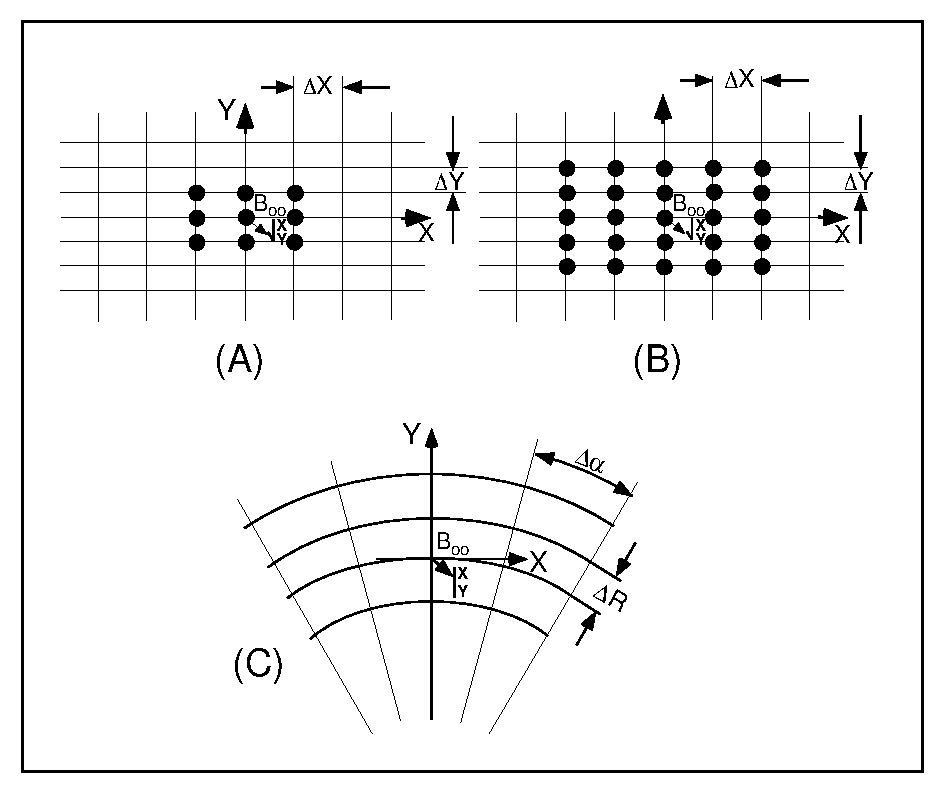
\includegraphics[width=15.5cm]{Fig3.ps}}
\hangcaption[Fig3]{
\label{fig3}Mesh in the $ (X,Y) $ plane. The grid is centered 
on the node which is closest to the actual position of the particle.\\
A~: Cartesian mesh, 9-point interpolation  grid.\\
B~: Cartesian mesh, 25-point interpolation grid.\\ 
C~: Polar mesh and moving Cartesian frame. 
}
\end{figure}


\noindent \zgou\ provides three types of polynomial
interpolation from the mesh (option \textsl{IORDRE\index{IORDRE}})~; namely, a second order interpolation, 
with either a 9- or a 25-point grid, or a fourth 
order interpolation with a 25-point  grid (Fig.~\ref{fig3}).  

\noindent If the 2-D field map is built up from  computer simulation, the grid in principle simply
aims at interpolating the field  and derivatives at a given point from its 9 or 25~neighbors.  
On the other hand if 
the map results from field measurements, the grid also has the virtue of  smoothing field 
fluctuations. 

\noindent The mesh may be defined in Cartesian coordinates, 
(Figs.~\ref{fig3}A and~\ref{fig3}B) or in polar coordinates (Fig.~\ref{fig3}C).   

\noindent The interpolation grid is centered on the node which is closest to
the projection in  the ($ X,Y) $ plane of the actual point of the trajectory. 

\noindent The interpolation polynomial is 

 \begin{equation}
	 B(X,Y,0) = A_{00} + A_{10}X + A_{01}Y + A_{20}X^2 + A_{11}XY + A_{02}Y^2
 	\label{eq2-4-4}
 \end{equation}
 %
 to the second order, or 

 \begin{equation}
	 \begin{aligned}
		 B(X,Y,0)  = 
		    & A_{00}+A_{10}X+A_{01}Y + A_{20}X^2 + A_{11}XY + A_{02}Y^2 \\
		%
		    & +  A_{30}X^3+A_{21}X^2Y + A_{12}XY^2 + A_{03}Y^3 \\
		%
		    & +  A_{40}X^4 + A_{31}X^3Y + A_{22}X^2Y^2 +A_{13}XY^3 + A_{04}Y^4 
	 \end{aligned}
 	\label{eq2-4-5}
 \end{equation}

to the  fourth order.  The coefficients $ A_{ij} $ are calculated by
expressions that 
minimize, with respect to $ A_{ij}$, the quadratic sum 

\begin{equation}
	S = \sum_{ij}(B(X,Y,0)-B_{ij})^2 
	\label{eq2-4-5b} %% 2-4-6
\end{equation}

The source code contains the explicit analytical 
expressions of the coefficients $A_{ij}$ solutions of the normal 
equations $\partial S / \partial A_{ij} = 0$.

\noindent The $ A_{ij} $ may then be identified with  the derivatives of 
$B(X,Y,0) $ at the central node of the grid 

\begin{equation}
	A_{ij} = \dfrac{1 }{ i!j!}\, \dfrac{\partial^{ i+j}B }{ \partial X^i\partial Y^j} \,(0,0,0) 
	\label{eq2-4-6}
\end{equation}
%
\noindent The derivatives of $ B(X,Y,0) $ with respect to $ X $ and $ Y$, at
the actual point 
$ (X,Y,0) $ are obtained by differentiation of the interpolation polynomial, 
which gives (\emph{e.g.},~from (\ref{eq2-4-4}) in the case of second order interpolation)
%
\begin{equation}
	\begin{aligned}
		\dfrac{ \partial B }{ \partial X} \,(X,Y,0)  
		   & =   A_{10}+2A_{20}X+A_{11}Y \\
		 \dfrac{\partial B }{ \partial Y}\, (X,Y,0) 
		   & =  A_{01}+A_{11}X+2A_{02}Y \\
		\text{etc.} 
	\end{aligned}
	\label{eq2-4-7}
\end{equation}
%
This allows stepping to the calculation of $ \vec  B(X,Y,Z) $ and its derivatives
as described in subsection~\ref{sec2.3.2} (eq.~\ref{eq2-3-3}).

\paragraph{The Special Case of Polar Maps} 
 
 \noindent In some optical elements (\eg, \textsl{POLARMES, DIPOLE[S]})
 the field is given in polar coordinates. It is thus necessary to transform the field and derivatives from the polar frame 
of the map, ($R,\alpha,Z$) to the Cartesian moving frame ($X,Y,Z$), Fig.~\ref{fig3}C.  This is done as  follows. 

\noindent In second order calculations the correspondence is (we note $B \equiv B_Z(Z=0)$)

 \begin{equation}
{\renewcommand{\arraystretch}{2}
	 \begin{array}{ll}
		 \dfrac{ \partial B }{ \partial X} 
		      &  = \dfrac{ 1 }{ R} \dfrac{\partial B }{ \partial \alpha} \\
		 \dfrac{ \partial B }{ \partial Y}
		      & = \dfrac{ \partial B }{ \partial R}\\
		\dfrac{\partial^2 B }{ \partial X^2} 
		      & =   \dfrac{ 1}{ R^2} \dfrac{\partial^2 B }{ \partial \alpha^ 2} 
		         + \dfrac{1 }{ R} \dfrac{\partial B}{\partial R}\\
		 \dfrac{ \partial^2 B }{ \partial X\partial Y}
		      & =  \dfrac{ 1 }{ R} \dfrac{\partial^ 2 B}{\partial \alpha \partial R}
		         - \dfrac{1 }{ R^2} \dfrac{\partial B }{ \partial\alpha}\\
		\dfrac{ \partial^2 B }{\partial Y^2}   
		      & =  \dfrac{ \partial^2 B }{ \partial R^2} \\
		 \dfrac{ \partial^3 B }{ \partial X^3} 
		      & = \dfrac{ 3 }{ R^2} \dfrac{\partial^2 B }{ \partial \alpha \partial R} 
		        - \dfrac{2 }{ R^3} \dfrac{\partial B }{ \partial \alpha}\\
		\dfrac{\partial^3 B }{ \partial X^2\partial Y} 
		      & = \dfrac{ -2 }{ R^3} \dfrac{\partial^2 B }{ \partial \alpha^2} 
		        - \dfrac{1}{ R^2} \dfrac{\partial B }{ \partial R} 
		        + \dfrac{1 }{ R} \dfrac{\partial^2 B }{\partial R^2}\\
		 \dfrac{ \partial^3 B }{ \partial X\partial Y^2} 
		      & =  \dfrac{ 2 }{ R^3} \dfrac{\partial B}{\partial \alpha} 
		         - \dfrac{2 }{ R^2} \dfrac{\partial^2 B }{ \partial \alpha\partial R}\\
		\dfrac{ \partial^3 B }{ \partial Y^3} 
		      &  =  0
	 \end{array} 
 	\label{eq2-4-8}}
 \end{equation}
 

%\newpage
  \noindent In fourth order calculations the relations above are pushed to fourth order in $X, ~ Y$  
 whereas 

{\renewcommand{\arraystretch}{2}
 \begin{equation}
	 \begin{array}{ll}
		 \dfrac{ \partial^3 B }{ \partial X^3} 
		     & =  \dfrac{ 1}{R^3} \, \dfrac{\partial^3 B}{\partial \alpha^3} 
		       + \dfrac{3 }{R^2} \, \dfrac{\partial^2 B }{\partial \alpha \partial R} 
		       - \dfrac{2 }{ R^3} \, \dfrac{\partial B }{ \partial \alpha}\\  %%
		 \dfrac{\partial^3 B }{ \partial X^2\partial Y} 
		     & =  \dfrac{1 }{ R^2} \, \dfrac{\partial^3 B }{\partial \alpha^ 2\partial R}
		       - \dfrac{2 }{ R^3} \, \dfrac{\partial^2 B }{ \partial \alpha^2} 
		       - \dfrac{1}{R^2} \, \dfrac{\partial B }{ \partial R} 
		       + \dfrac{1 }{ R} \, \dfrac{\partial^2 B }{ \partial R^2} \\  %%
		 \dfrac{ \partial^3 B }{ \partial X\partial Y^2} 
		     & =  \dfrac{ 1 }{ R} \, \dfrac{\partial^3 B }{ \partial \alpha \partial R^2} 
		       + \dfrac{2 }{ R^3} \, \dfrac{\partial B }{\partial \alpha}  
		       - \dfrac{2 }{R^2} \, \dfrac{\partial^ 2B }{ \partial \alpha \partial R} \\ %%
		 \dfrac{ \partial^3 B }{ \partial Y^3}
		     & =  \dfrac{ \partial^3 B }{ \partial R^3} \\ %%
		\dfrac{\partial^4 B }{ \partial X^4}
		     & = \dfrac{ 1}{ R^4} \, \dfrac{\partial^4 B }{ \partial \alpha^4} 
		       - \dfrac{8 }{ R^4} \, \dfrac{\partial^2 B }{ \partial \alpha^2} 
		       + \dfrac{6 }{ R^3} \, \dfrac{\partial^3 B }{ \partial\alpha^2\partial R} 
		       + \dfrac{3 }{ R^2} \, \dfrac{\partial^2 B }{ \partial R^2} 
		       - \dfrac{3}{ R^3} \, \dfrac{\partial B }{ \partial R} \\ %%
	     \dfrac{ \partial^4 B }{ \partial X^3\partial Y}
	         & =   \dfrac{ 1 }{ R^3} \, \dfrac{\partial^ 4B }{\partial \alpha^ 3\partial R} 
	           - \dfrac{3 }{ R^4} \, \dfrac{\partial^ 3B }{ \partial\alpha^ 3} 
	           + \dfrac{3 }{ R^2} \, \dfrac{\partial^3 B }{ \partial \alpha \partial R^2} 
	           - \dfrac{8 }{ R^3} \, \dfrac{\partial^2 B }{ \partial \alpha \partial R} 
	           + \dfrac{6 }{ R^4} \, \dfrac{\partial B }{ \partial \alpha} \\   %%
	    \dfrac{ \partial^4 B}{ \partial X^22 Y^2} 
	         & =  \dfrac{ 1 }{ R^4} \, \dfrac{\partial^2 B }{ \partial \alpha^ 2} 
	           - \dfrac{4 }{ R^3} \, \dfrac{\partial^3 B }{ \partial \alpha^ 2\partial R} 
	           - \dfrac{2 }{ R^2} \, \dfrac{\partial^2 B }{ \partial R^2} 
	           + \dfrac{2 }{ R^3} \, \dfrac{\partial B }{ \partial R} 
	           + \dfrac{1 }{ R^2} \, \dfrac{\partial^4 B }{ \partial \alpha^2\partial R^2} 
	           + \dfrac{1 }{ R} \, \dfrac{\partial^3 B }{ \partial R^3}\\     %%
	     \dfrac{ \partial^4 B }{ \partial X\partial Y^3} 
	         & = \dfrac{ 1 }{ R} \, \dfrac{\partial^4 B }{\partial \alpha \partial R^3} 
	           - \dfrac{3 }{ R^2} \, \dfrac{\partial^3 B }{ \partial \alpha \partial R^2} 
	           + \dfrac{6 }{ R^3} \, \dfrac{\partial^2 B }{ \partial \alpha\partial R} 
	           - \dfrac{6 }{ R^4} \, \dfrac{\partial^4 B }{ \partial \alpha^ 4} \\  %%
	     \dfrac{ \partial^4 B }{ \partial Y^4}
	         & =   \dfrac{ \partial^4 B }{ \partial R^4}
	 \end{array} 
	\label{eq2-4-9}
\end{equation}  }
 
\medskip 


\noindent \textbf{NOTE~:} In case  a particle goes beyond the limits of the 
 field map, the field and its derivatives are extrapolated 
using  a grid at the border of the map,  which is the closest to the actual position of the 
particle.         
The flag \IEX\index{IEX@{\IEX}} attached to the particle (section~\ref{sec4.6.6}, p.~\pageref{sec4.6.6}) 
is then given the value $-1$. 




\subsubsection{Arbitrary 2-D Map, no Symmetry} \label{sec2.4.3}

The map is assumed to describe the field $ \vec  B(B_X,B_Y,B_Z) $ in the $ (X,Y) $ 
plane at elevation $ Z_0 $. It provides the components $ B_{X,ij}$, $
B_{Y,ij}$,  $ B_{Z,ij} $ at 
each node $ (i,j) $ of a 2-D mesh. 

\noindent The value of $ \vec  B $ and its derivatives at the projection $
(X,Y,Z_0) $ of the actual position $ (X,Y,Z) $ 
of a particle is obtained by means of  
 (parameter \textsl{IORDRE} in  keyword data list - see for instance \textsl{MAP2D,~MAP2D-E})
either a second degree polynomial interpolation from a $3 \times 3$~points grid (\textsl{IORDRE}=2),  
or a fourth degree polynomial interpolation from a $5 \times 5$~points grid (\textsl{IORDRE}=4),  
centered at the node $(i,j) $  closest to the position $ (X,Y)$. 

\noindent To second order for instance 

 \begin{equation}
	 B_{\ell} (X,Y,Z_0)=A_{00} +A_{10} X +A_{01} Y +A_{20} X^2 +A_{11} X Y +A_{02} Y^2
 	\label{eq2-4-10}
 \end{equation}
 %
where $ B_{\ell} $ stands for any of the three components $ B_X$, 
$B_Y $ or $ B_Z $. 
Differentiating then gives the derivatives

\begin{equation}
	\begin{aligned}
		 \dfrac{ \partial B_{\ell} }{ \partial X} \,(X,Y,Z_0)
		     & =   A_{10} +2 A_{20} X + A_{11} Y  \\
		\dfrac{ \partial^2 B_{\ell} }{ \partial X\partial Y}\, (X,Y,Z_0)
		     & =  A_{11} \\
		\text{etc.}
	\end{aligned}
	\label{eq2-4-11}
\end{equation}


\noindent Then follows a procedure of extrapolation from $ (X,Y,Z_0) $ to
the actual position $ (X,Y,Z)$, based on Taylor series development. 

\noindent No special symmetry is assumed, which allows the treatment of 
arbitrary field distribution (\emph{e.g.}, solenoid, helical snake). 


%%%%%%%%%%%%%%figure%%%%%%%%%%%%%%
\begin{figure}[h]   %%[H]
%\vspace{11 truecm}
%%%Figure 4
\centerline{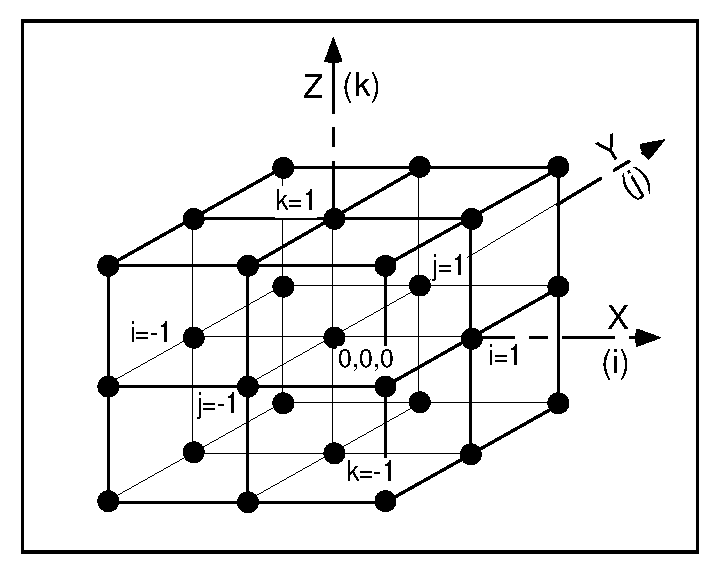
\includegraphics[width=14cm]{Fig4.ps}}
\hangcaption{\label{fig4}A 3-D 27-point  grid is used for
interpolation of magnetic or electric fields and  
derivatives up to second order.  The central node of the grid $ (i=j=k=0) $ is
 the closest to the actual position of the particle.} 
\end{figure}




\subsubsection{3-D Field Map} \label{sec2.4.4}

When using a 3-D field map, the vector field $ \vec  B(X,Y,Z) $ and its derivatives necessary
for the calculation of position and velocity of the particle are obtained 
via  second degree  polynomial interpolation, 

\begin{equation}
\!\!	B_{\ell} (X,Y,Z) = A_{000} + A_{100} X + A_{010} Y + A_{001} Z + 
	A_{200} X^2 + A_{020} Y^2  
	+     A_{002} Z^2 + A_{110} X Y + A_{101} X Z + A_{011} Y Z
	\label{eq2-4-12}
\end{equation}

\noindent$ B_{\ell} $ stands for any of the three components, $ B_X, $ $ B_Y $
or $ B_Z $.  By 
differentiation of $ B_{\ell} $ one gets 

\begin{equation}
	\begin{aligned}
		 \dfrac{ \partial B_{\ell} }{ \partial X} 
		    & =  A_{100} + 2 A_{200} X + A_{110} Y + A_{101} Z\\
		\dfrac{\partial^2 B_{\ell}}{ \partial X^2} 
		    & =  2 A_{200} 
	\end{aligned}
	\label{eq2-4-13}
\end{equation}
%
 and so on up to  second order derivatives with respect to  $X$, $ Y $ or $ Z $. 
 
\noindent The interpolation involves a $ 3  \times   3  \times   3$-point 
parallelepipedic grid (Fig.~\ref{fig4}),   
the origin of which is positioned at the node of the 3-D field map which is 
closest to the actual position of the particle. 
\medskip

\noindent Let $ B^{\ell}_{ijk} $ be the value of the --- measured or computed ---
magnetic field at each one of the 27~nodes of the 3-D grid ($ B^{\ell} $ stands for  
$ B_X$, $ B_Y $ or $ B_Z $), and $ B_{\ell} (X,Y,Z) $ be the value at a
position $ (X,Y,Z) $ 
with respect to the central node of the 3-D grid. Thus, any 
coefficient $ A_i $ of the polynomial expansion of $ B_{\ell} $ is obtained by
means of expressions that minimize, with respect to $ A_i $, the sum
%
\begin{equation}
	S = \sum_{ijk} \left(B_{\ell} (X,Y,Z)-B^{\ell}_{ijk} \right)^2 
	\label{eq2-4-14} %% reel~: 2-4-15
\end{equation}
%
 where the indices $ i$, $j $ and $ k $ take the values -1, 0 or +1 so as
to sweep the 3-D grid. The source code contains the explicit analytical 
expressions of the coefficients $A_{ijk}$ solutions of the normal 
equations $\partial S / \partial A_{ijk} = 0$.





\clearemptydoublepage

\section[SPIN TRACKING]{SPIN TRACKING\index{spin tracking}~\protect}\label{sec3}   %%% [7]

%%% chgt de numerotation des equations pour ne pas avoir 3.0.1 %%%
%% \renewcommand\theequation{\thesubsection.\arabic{equation}}
%\renewcommand\theequation{\thesection.\arabic{equation}}
%\makeatletter
%\@addtoreset{equation}{section}
%\makeatother
%%%

Spin motion tracking was  implemented in \zgou\ in the SATURNE years~\cite{Biblio7}, 
it has been since  used in a number of studies, including the transport of polarized muons 
 in the Neutrino Factory~\cite{polarNuFact}, 
polarization survival in the superB project~\cite{polarSuperB}, 
studies on proton polarization with helical snakes
at AGS~\cite{polarAGS} and RHIC~\cite{polarRHIC},  
and in the magic-energy electrostatic ring of the proton-EDM project~\cite{polarPEDM}. 


\subsection{Introduction}

The precession  of the spin $ \vec  S $ of a charged particle in electric and magnetic fields 
is governed by the Thomas-BMT first order differential equation~\cite{Biblio8}       %%%%[8] 

\begin{gather}
	\dfrac{d\vec  S }{ dt} = \dfrac{q }{  m} \, \vec  S\times\vec  \omega
	     \label{eq3-1-S}  \\
\intertext{with, in the laboratory frame, }
	\vec  \omega  = (1+\gamma G)\vec  b + G(1-\gamma )\vec  b_{\paral} + \gamma(G + \dfrac{1}{1+\gamma})  \dfrac{\vec e \times \vec v}{c^2}   \label{eq3-2-S}  
\end{gather}

\noindent $t$, $ q$, $m$, $c$, $\gamma$ and $ G $ are respectively the time, charge, 
relativistic mass, speed of light, Lorentz relativistic factor  and anomalous magnetic moment of the 
particle, $\vec b$ and $\vec e$ are the fields in the laboratory, $ \vec  b_{\paral} $ is the component of $ \vec  b $ 
parallel to the velocity $ \vec  v $ of the particle. 

\noindent Equation~(\ref{eq3-1-S}) is normalized by introducing the same notation 
as for the Lorentz equation, page~\pageref{eq2-2-2}, 
namely  $ b=\parallel\vec  b\parallel $, $v=||\vec v||$, $ \vec v= v \vec u$, 
$ ds=vdt $ the differential path, $ \dfrac{\gamma mv }{ q} = \Br $  the rigidity of the particle, 
whereas $ \vec  S^{\,\prime} = \dfrac{d\vec  S }{ ds} = \dfrac{1 }{ v}\dfrac{d\vec  S }{ dt} $ 
 is the derivative of the spin with respect to the path.  This yields

%\noindent Introducing in addition the normalized fields  $ \vec  B= \dfrac{\vec  b }{ \Br} $, 
%$ \vec B_{\paral} = \dfrac{\vec  b_{\paral} }{ \Br} $, $ \vec  E= \dfrac{\vec  e }{ \Br} $,  
% eq.~(\ref{eq3-1-S}) can be re-written in the simpler form 

 \begin{equation}
    (B\rho) \, \vec S^{\,\prime}  = \vec  S \times  \vec  \omega ~ ~ ~ ~ ~ \textrm{or} ~ ~ ~ ~ 
    \vec S^{\,\prime}  = \vec  S \times  \vec  \Omega
 	\label{eq3-4-S}
 \end{equation}
 
\noindent where, noting $\vec B = \vec b/\Br$, $\vec E = \vec e/\Br$,

\begin{equation}
	\vec  \Omega  = \dfrac{\vec \omega }{ \Br}  = (1+\gamma G)\vec  B +
	G(1-\gamma )\vec  B_{\paral} + \dfrac{\beta \gamma}{c}(G + \dfrac{1}{1+\gamma}) \vec E \times \vec u  
	\label{eq3-3-S}
\end{equation}

\noindent This equation is solved in the same way as the reduced Lorentz equation~(\ref{eq2-2-3}). 
From the values of the  precession factor $ \vec  \omega (M_0) $ and spin $\vec  S(M_0) $ 
of the particle at position $ M_0 $, the spin $ \vec  S(M_1)$ 
at position $ M_1 $, following a displacement $ \Delta s$ (fig.~\ref{fig2}), is obtained from truncated 
Taylor expansion 

 \begin{equation}
	 \vec  S(M_1) \approx \vec  S(M_0)+ \dfrac{d\vec  S }{ ds} (M_0)\, \Delta s
	 + \dfrac{d^2\vec  S }{ds^2} \,(M_0) \dfrac{\Delta s^2 }{ 2} 
	 + \dfrac{d^3\vec  S }{ ds^3} \,(M_0) \dfrac{\Delta s^3 }{ 3!}
	+ \dfrac{d^4\vec  S }{ ds^4}\, (M_0) \dfrac{\Delta s^4 }{ 4!}
	+ \dfrac{d^5\vec  S }{ ds^5}\, (M_0) \dfrac{\Delta s^5 }{ 5!}
 	\label{eq3-5-S}
 \end{equation}
 


\subsection{Integration in Magnetic Fields} \label{secSpin.2.1}  

In purely magnetic fields  $ \vec  e=0 $ thus eq.~(\ref{eq3-3-S}) reduces to

 \begin{equation}
 \vec \Omega_b = (1+\gamma G)\vec  B + G(1-\gamma )\vec  B_{\paral} 
 \label{eq3-2-B}  
\end{equation}

\noindent $\vec S$ and its derivatives $ \vec  S^{(n)} = d^n\vec  S / ds^n $ 
satisfy the  recursive differentiation relations

 \begin{equation}
	 \begin{aligned}
               \vec   S^{\,\prime}  & = \vec  S \times  \vec  \Omega_b \\
		\vec  S^{\,\prime\prime} 
		      &  =\vec  S^{\,\prime} \times\vec  \Omega_b +\vec  S\times\vec  \Omega_b ^\prime \\
		\vec  S^{\,\prime\prime\prime}
		      &  =\vec  S^{\,\prime\prime} \times\vec  \Omega_b +2\vec  S^{\,\prime} \times\vec  \Omega_b ^\prime 
		           +\vec S\times\vec  \Omega_b^{\prime\prime} \\
                 &  \textrm{etc.}
%		\vec  S^{\quaprime} 
%		      & =\vec S^{\,\prime\prime\prime} \times\vec  \Omega_b 
%		          +3\vec  S^{\,\prime\prime} \times\vec \Omega_b^\prime 
%		          +3\vec  S^{\,\prime} \times\vec  \Omega_b^{\prime\prime} 
%		          +\vec S\times\vec  \Omega_b^{\prime\prime\prime}
	 \end{aligned}
 	\label{eq3-6-S}
 \end{equation}
 
 \noindent  with the derivatives $ d^n \vec  \Omega_b / ds^n $  obtained by differentiation of  eq.~(\ref{eq3-2-B}). 
 This requires   $ \vec  B_{\paral} $ and  derivatives, obtained in the following way, 
\begin{equation}
	\begin{aligned}
		\vec  B_{\paral} 
		     & = (\vec  B \cdot\vec  u)\, \vec  u \\
		\vec  B^{\,\prime}_{\paral}  
		     & = (\vec B^{\,\prime} \cdot\vec  u+\vec  B\cdot\vec  u^{\,\prime} )\,\vec  u
		       +(\vec  B\cdot\vec  u)\,\vec u^{\,\prime} \\
		\vec B^{\,\prime\prime}_{\paral}  
		     & = (\vec  B^{\,\prime\prime} \cdot\vec  u+2\vec B^{\,\prime} \cdot\vec  u^{\,\prime} 
		       +\vec  B\cdot\vec  u^{\,\prime\prime} )\, \vec  u
		       +2(\vec B^{\,\prime} \cdot\vec  u+\vec  B\cdot\vec  u^{\,\prime} )\,\vec  u^{\,\prime} 
		       +(\vec  B\cdot\vec u)\,\vec  u^{\,\prime\prime}\\
		&\text{\textrm{etc.}}
	\end{aligned}
	\label{eq3-7-S}
\end{equation}
\noindent The quantities $ \vec  u$,  $ \vec  B $ and their  derivatives
as involved in these equations are known, being sub-products of the integration of the  motion of the 
particle, eqs.~(\ref{eq2-2-6}, \ref{eq2-2-7}) p.~\pageref{eq2-2-6}.




\subsection[Integration in Electric Fields]{Integration in Electric Fields}

        \label{sec2.2.2-E} %%%% 2.2.2.[3]

In purely electric fields  $ \vec  b=0, $ thus eq.~(\ref{eq3-2-S}) reduces to
\begin{gather}
 \omega_e = \dfrac{\beta \gamma}{c}(G + \dfrac{1}{1+\gamma}) \, \vec e\times \vec u  \label{eq3-2-E}  
\end{gather}

\noindent $\vec S$ and its derivatives $ \vec  S^{(n)} = d^n\vec  S / ds^n $ 
satisfy the  recursive differentiation relations

\begin{equation}
	\begin{array}{ll}
	 \Br \, \vec S^{\,\prime} &= \vec  S \times \vec \omega_e \\
		(\Br)^\prime \vec  S^{\,\prime} 
		     +\Br \vec  S^{\,\prime\prime}  & =  \vec S^{\,\prime}  \times \vec \omega_e + \vec  S \times \vec \omega_e'       \\
		(\Br)^{\prime\prime}\vec  S^{\,\prime}
		      + 2(\Br)^\prime \vec  S^{\,\prime\prime} 
		      +\Br \vec  S^{\prime\prime\prime}  & =
   \vec  S^{\,\prime\prime}  \times \vec \omega_e + 2\vec S^{\,\prime}  \times \vec \omega_e^{\,\prime}  + \vec  S^{\,\prime}  \times \vec \omega_e''       \\
          ~ ~  ~    \textrm{etc.}
	\end{array}
	\label{eq2-2-9-E}
\end{equation} 
\noindent that provide the derivatives $ d^n\vec  S / ds^n$ needed in the Taylor 
expansion~(eq.~\ref{eq3-5-S}).  
 The derivatives $ (\Br)^{(n)} =   d^n(\Br ) / ds^n $  above are a sub-product of the integration of the 
force law (eq.~\ref{eq2-2-15}). The derivatives of $\omega_e$ (eq.~\ref{eq3-2-E}) are obtained 
by recursive differentiation, 

\begin{equation}
	\begin{array}{l}
 \vec \omega_e' = \left( \dfrac{\beta \gamma}{c}(G + \dfrac{1}{1+\gamma})\right)' \vec e \times \vec u   
  +   \dfrac{\beta \gamma}{c}(G + \dfrac{1}{1+\gamma})\left( \vec e \times \vec u   \right)'  \\
 \vec \omega_e'' = \left( \dfrac{\beta \gamma}{c}(G + \dfrac{1}{1+\gamma})\right)'' \vec e \times \vec u   
  +  2 \left( \dfrac{\beta \gamma}{c}(G + \dfrac{1}{1+\gamma}) \right)' \left( \vec e \times \vec u   \right)'  
  +   \dfrac{\beta \gamma}{c}(G + \dfrac{1}{1+\gamma})\left( \vec e \times \vec u   \right)''  \\
          ~ ~ ~       \textrm{etc.}
	\end{array}
	\label{eqOmega-E}
\end{equation} 

\noindent  The quantities $ \left( \dfrac{1}{1+\gamma} \right)^{(n)}$  in the $(\omega_e)^{(n)}$ above 
are obtained as follows. 

\noindent From $\gamma^2 = 1/(1-\beta^2)$ it comes $(\gamma+1)(\gamma-1) \beta^2/(1-\beta^2)$ and then
$$\dfrac{1}{1+\gamma} = \left( \dfrac{1}{\beta} -1 \right) \left( \dfrac{1}{\beta} +1 \right) (\gamma-1)$$
which is easily differentiated, recursively, 
\begin{equation}
	\begin{array}{lcc}
\left( \dfrac{1}{1+\gamma}\right)' &= &
\left( \dfrac{1}{\beta} \right)' \left( \dfrac{1}{\beta} +1 \right) (\gamma-1)  +
\left( \dfrac{1}{\beta} -1 \right) \left( \dfrac{1}{\beta} \right)' (\gamma-1) + 
\left( \dfrac{1}{\beta} -1 \right) \left( \dfrac{1}{\beta} +1 \right) \gamma' \\
\left( \dfrac{1}{1+\gamma}\right)'' &= &
\left( \dfrac{1}{\beta} \right)'' \left( \dfrac{1}{\beta} +1 \right) (\gamma-1)  +
\left( \dfrac{1}{\beta} -1 \right) \left( \dfrac{1}{\beta} \right)'' (\gamma-1) + 
\left( \dfrac{1}{\beta} -1 \right) \left( \dfrac{1}{\beta} +1 \right) \gamma''  +\\
&& 2 \left( \dfrac{1}{\beta} \right)' \left( \dfrac{1}{\beta}\right) (\gamma-1)  + 
2 \left( \dfrac{1}{\beta}  \right)' \left( \dfrac{1}{\beta} \right)' (\gamma-1) + 
 2 \left( \dfrac{1}{\beta} -1 \right) \left( \dfrac{1}{\beta} \right)' \gamma' \\
              &  \textrm{etc.}
	\end{array}
	\label{eqGamma-E}
\end{equation} 

\noindent The interest of that formulation is that the $\left( \dfrac{1}{\beta} \right)^{(n)}$ are already known from the particle dynamics, eq.~(\ref{eq2-2-17}), 
as well as the derivatives 
$$	\dfrac{ d^{n+1} \gamma }{ds^{n+1}} = \dfrac{q}{m} \, \dfrac{ d^n (\vec  e\cdot\vec  u) }{ ds^n}$$

\noindent following eq.~(\ref{eq2-2-16}), whereas the $d^n (\vec  e\cdot\vec  u)/ ds^n$ are given by eq.~(\ref{eqEscalu}).


 \subsection{Integration in Combined Electric and Magnetic Fields} \label{sec2.2.3-S}%%%% 2.2.3.

 When both $ \vec  e $ and $ \vec  b $ are non-zero, the complete 
 eqs.~(\ref{eq3-4-S},~\ref{eq3-3-S}) must be considered. 

\noindent The precession vector (eq.~\ref{eq3-3-S}) and its derivatives 
can be split into independent, magnetic and electric components, namely
$$  \vec \omega = \vec \omega_b + \vec \omega_e , ~ ~ \vec \omega^{\,\prime} = \vec \omega_b^{\,\prime} + \vec \omega_e^{\,\prime}  , ~ ~ ~ \textrm{~ ~  ~ etc.}$$
 As a consequence, 
the  spin vector $\vec S(s)$ and its derivatives  at location $M_0$ prior to a $\Delta s$  push to 
location $M_1$ (fig.~\ref{fig2})
can be  obtained by linear superposition of the separate solutions 
for the magnetic case~(eq.~\ref{eq3-6-S}) and for the electric case~(eq.~\ref{eq2-2-9-E}), namely

{%\small
\begin{equation}
	\label{eq2-2-9-EB}
	\begin{array}{lll}	 
	 \multicolumn{3}{l}{\Br \, \vec S^{\,\prime} =}   \\
 & \hspace{-8mm} \vec  S \times \vec \omega_b  
 & + \vec  S \times \vec \omega_e    \\[1ex]
    	 \multicolumn{3}{l}{\Br\vec  S^{\,\prime\prime} =}  \\
 &  \hspace{-8mm}  \vec  S^{\,\prime}  \times \vec \omega_b + \vec  S \times \vec \omega_b^{\,\prime} 
 &  +    \vec  S^{\,\prime}  \times \vec \omega_e + \vec  S \times \vec \omega_e^{\,\prime} 
          - (\Br)^\prime \vec  S^{\,\prime}    \\[1ex]
   	 \multicolumn{3}{l}{\Br\vec  S^{\prime\prime\prime} =}  \\
  & \hspace{-8mm} \underbrace{
\vec  S^{\,\prime\prime}  \times \vec \omega_b + 2\vec  S^{\,\prime} \times \vec \omega_b^{\,\prime}   + \vec S \times \vec \omega_b^{\,\prime\prime} 
              }_{\textrm{Magnetic field component, eq.~(\ref{eq3-6-S})}}  
&   \underbrace{ 
     + \vec  S^{\,\prime\prime}  \times \vec \omega_e + 2\vec  S^{\,\prime} \times \vec \omega_e^{\,\prime}   + \vec S \times \vec \omega_e^{\,\prime\prime}    
    -\left(  (\Br)^{\prime\prime}\vec  S^{\,\prime}
		      + 2 (\Br)^\prime \vec  S^{\,\prime\prime}  \right) 
               }_{\textrm{Electric field component, eq.~(\ref{eq2-2-9-E})}}     \\
          ~ ~  ~      \textrm{etc.}
	\end{array}
\end{equation} 
}%small

\noindent The process is then completed by applying the $\Delta s$ push, eq.~(\ref{eq3-5-S}). 




\clearemptydoublepage

\section{SYNCHROTRON RADIATION }\label{secN4}\index{synchrotron radiation} 

%%% on a de nouveau une numerotation des equations 4.1.1 %%%
\renewcommand\theequation{\thesubsection.\arabic{equation}}
\makeatletter
\@addtoreset{equation}{subsection}
\makeatother

\zgoubi\ provides the  simulation of two distinct types of synchrotron radiation (SR) manifestations 
 namely, on the one hand energy loss by stochastic emission of photons and the ensuing perturbation 
on particle dynamics  and, on the other hand the radiated electro-magnetic field impulse and 
its spectral-angular energy density as observed in the laboratory. 

\medskip

\noindent {\bf SR loss simulation} was first installed in \zgou\ in view of beam dynamics studies in the beam delivery system of the 
Next Linear Collider~\cite{FMSEA-00-01}, based on a  method developed in the frame 
of the ELFE project (``EU Lab. For Electrons'')~\cite{SRLossGL,DYNAC,ELFE}. 
It was next used for including damping effects in beam studies 
regarding various electron-ring and recirculator projects~\cite{polarSuperB,SRLossBench}. 

\medskip

\noindent {\bf SR electromagneitc impulse and spectrum} computation was first installed in \zgou\ for the 
study of interference effects at the LEP beam diagnostics miniwiggler~\cite{FMSL/94-22}. 
These simulation tools were next used to design the LHC SR beam diagnostics systems, 
located in the IR4 RF section~\cite{FMLPYellow}. 



\subsection{Energy Loss and  Dynamical Effects}\label{secSRLoss}

Most of the contents of the present section are drawn from Ref.~\cite{FMSEA-00-01}\label{SRLoss}.

\medskip

\noindent Given a particle wandering in the magnetic field of an arbitrary optical element or field 
map, \zgoubi\ computes the energy loss undergone, and its 
effect on the particle motion. The energy loss is calculated  in a  classical manner, by invoking 
two random processes that accompany the emission of a photon  namely, \\
\indent - the probability of emission, \\
\indent - the energy of the photon. 

\noindent The effects on the dynamics of the emitting particle 
 either account for the sole  alteration of its  energy, or, if requested, include the angle kick.
Particle position is supposed not to  change upon emission of a photon. These calculations 
 and ensuing dynamics corrections are performed at 
 each integration step. In a practical manner, this requires 
 centimeters  to tens of centimeters steps in smoothly varying magnetic fields (a quantity to 
be determined before any simulation, from convergence trials). 

\medskip 


\noindent Main aspects of the method are developed in the following. 


%\newpage 

\paragraph{Probability of Emission of a Photon}

Given that the number of photons emitted within a step $\Delta s$ can be very small  (units or fractions 
of a unit)\footnote{For instance, a $1\,$GeV electron will emit about $20.6$ photons per radian~; an 
 integration step size $\Delta s =0.1\,$m upon $\rho=10\,$m bending radius results in 0.2 photon  
per step.} a Poisson probability law 

\begin{equation}
	\label{EqPoiss}
 p(k) = \dfrac{\lambda^k}{k!} \exp(-\lambda)
\end{equation}
%
is considered. $k$ is the number of photons emitted over a $\Delta \theta$ (circular) arc of 
trajectory  such that, the average number of photons per radian expresses as\footnote{This leads for 
instance, in the case of electrons, to the classical formula $\lambda/\Delta \theta \approx
129.5$E(GeV)$/2\pi\approx \gamma/94.9$.}

\begin{equation}
        \label{EqPoissMean}
 \lambda = \dfrac{20 e r_0 }{8 \hbar \sqrt{3}  } \beta^2 \Br  \dfrac{\Delta s}{\rho}
\end{equation}
%
where $r_0=e^2/4\pi \epsilon_0 m_0 c^2$ is the classical radius of the particle of rest-mass $m_0$, 
$e$ is the elementary 
charge, $\hbar = h/2\pi , h$ is the Planck constant, $\beta = v/c$, $\Br$ is the particle 
stiffness. $\lambda$ is evaluated at each integration step from the current values $\beta$, $\Br$ 
and $\Delta s$,  then a value of $k$ is drawn by a rejection method.  


\paragraph{Energy of the Photons}

These k photons are assigned energies $\epsilon=h\nu$ at random, in the following way. The cumulative 
distribution of the energy probability law $p(\epsilon/\epsilon_c)d\epsilon/\epsilon_c$  
(\ie, the probability of emission of a photon with  energy in  $[0,\epsilon]$) writes~\footnote{From 
a practical viewpoint, the value of the magnetic field first computed for a 
one-step push of the particle  (eqs.~\ref{eq2-2-4},~\ref{eq2-2-6}) is next used to  obtain  
$\rho$ and perform SR loss corrections afterwards.} 

\begin{equation}
\label{EqSK53}
 \mathcal{P}(\epsilon/\epsilon_c) = \dfrac{3}{5\pi} \int_0^{\epsilon/\epsilon_c} \dfrac{d\epsilon}{\epsilon_c} \int_{\epsilon/\epsilon_c}^\infty K_{5/3}(x) dx
%\mathcal{P}(\epsilon/\epsilon_c) = \dfrac{3}{5\pi}                           \int_0^{\epsilon/\epsilon_c} K_{5/3}(x) dx
\end{equation}
%
\begin{wrapfigure}{r}{9cm}
  \begin{center} 
\vspace{-2mm}
\includegraphics*[bbllx=20,bblly=100,bburx=550,bbury=450,width=6cm]{G.eps}
\vspace{-0mm}

 {\small \centering 
       Cumulative energy distribution   $\mathcal{P}(\epsilon/\epsilon_c)$. }
  \end{center}
\end{wrapfigure}
where $K_5/3$ is a modified Bessel function and, $\epsilon_c= \hbar \omega_c$, 
$\omega_c=2 \pi \times 3 \gamma^3 c / 2 \rho$ being the critical frequency  in 
the presence of bending radius $\rho$~;  $\omega_c$ is evaluated at each integration step from 
the current values $\gamma$ and $\rho$, in other words, this energy loss calculation 
assumes constant  magnetic field  over the trajectory arc $\Delta s$. 
In the low frequency region $(\epsilon/\epsilon_c \ll 1)$ it can be approximated by 

\begin{equation}
\label{EqSK53Low}
\mathcal{P}(\epsilon/\epsilon_c) = \dfrac{12 \sqrt{3}}{2^{1/3} \, 5 \, \Gamma(\dfrac{1}{3})}  
(\dfrac{\epsilon}{\epsilon_c})^{1/3}
\end{equation}
%
\noindent  About $40$ values of $\mathcal{P}(\epsilon/\epsilon_c)$ computed from eq.~\ref{EqSK53}~\cite{VOKostroun}, 
honestly spread  over a range $\epsilon/\epsilon_c \leq 10$ are  tabulated 
in \zgoubi\ source file (see figure). In 
order to get $\epsilon/\epsilon_c$, first a random value $0<\mathcal{P}<1$ is generated uniformly, 
then  $\epsilon/\epsilon_c$ is drawn either  by simple inverse linear interpolation 
 of the tabulated values if $\mathcal{P}>0.26$ (corresponding to 
$\epsilon/\epsilon_c>10^{-2}$), 
or, if $\mathcal{P}<0.26$ from eq.~\ref{EqSK53Low} that gives 
 $\epsilon/\epsilon_c= \bigl( \dfrac{5 \, 2^{1/3} \Gamma(\dfrac{1}{3})}{12 \sqrt{3} \mathcal{P}}\bigr)^3$ 
 with precision no less than 1$\%$ at  $\mathcal{P}\rightarrow 0.26$. 

\bigskip


\noindent When SR loss tracking is requested, several optical elements that contain a dipole 
magnetic field component (\emph{e.g.}, \textsl{MULTIPOL}, \textsl{BEND}) provide a printout of various 
 quantities related to SR emission, as drawn from classical theoretical 
expressions, such as for instance, \\
- energy loss per particle $\Delta E(eV)= \dfrac{2}{3}r_0 c \gamma^3 B(T) \Delta \theta$,   with $B$ 
the dipole field  exclusive of any other multipole component 
in the magnet, $\Delta \theta$  the total deviation as calculated from $B$, from the 
magnet length, and from the reference rigidity \BORO\ (as defined with, \eg, \textsl{[MC]OBJET}) \\
-  critical energy $\epsilon_c(eV)=\dfrac{3 \gamma^3 c}{2 \rho} \dfrac{\hbar}{e}$, with 
$\rho =$\BORO$/B$ \\
- average energy of the photons radiated $<\epsilon> = \dfrac{8}{15 \sqrt{3}} \epsilon_c$, \\ 
- \rms\ energy of radiated photons $\epsilon_{rms} = 0.5591 \epsilon_c$, \\
- number of radiated photons per particle  $N = \Delta E /<\epsilon>$.  

\noindent This is done in order to facilitate verifications, since on the other hand statistics 
regarding those values are drawn from the tracking and may be printed using  the dedicated 
keyword \textsl{SRPRNT}. 



\bigskip

\noindent Finally, upon user's request as well,  SR loss can be limited to particular classes of optical 
elements, for instance dipole magnets alone, or dipole + quadrupole magnets, etc. This option 
is made available in order to allow further inspection, or easier comparison with other codes, for instance. 



\subsection{Spectral-Angular Radiated Densities}\label{secSRSpec}

Most of the content in the present section is drawn from Refs.~\protect\cite{FMSL/94-22,FMLPYellow,PALowFreq}.

\medskip

\noindent The ray-tracing procedures provide the ingredients necessary 
for the determination of the electric field radiated by the particle subject to
acceleration, as shown in Fig.~\ref{newfig5}, this is developed in section~\ref{secN4.1}. 
These ingredients further allow calculating the spectral-angular density of the 
radiation\footnote{These calculations have been installed in the 
post-processor  \textbf{zpop}. \index{zpop}},   this is developed in section~\ref{secN4.2}. 


%%%%%%%%%%%%%%figure%%%%%%%%%%%%%%
%\vspace{1cm}
\begin{figure}[h]
%\vspace{4.5 truecm}
%%%Figure 6
\centering
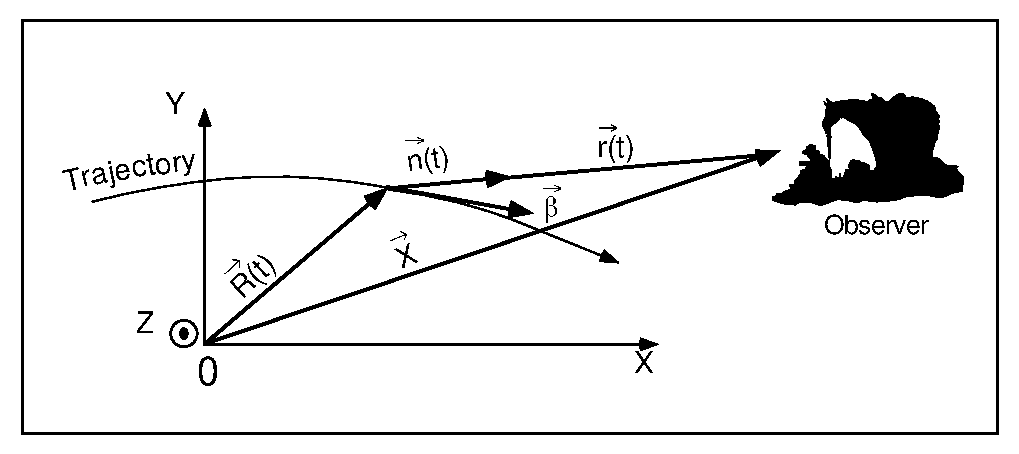
\includegraphics[width=16cm]{NewFig5.ps} 
{\setlength{\captionwidth}{15cm}
\hangcaption[NewFig 6]{\label{newfig5}A scheme of the reference frame in 
\zgou\ together with the vectors entering
in the definition of the electric field radiated by the accelerated particle~:\\
$(x,y)$~: horizontal plane~;~$z$~: vertical axis.\\
$\vec{R}(t)$ = particle position in the fixed frame $(O, x, y, z)$~;\\
$\vec{X}$ (time-independent) = position of the observer in the  $(O, x, y, z)$ frame~;\\
$\vec{r}(t) = \vec{X} - \vec{R}(t)$ = position of the particle with respect to
the observer~;\\
$\vec{n}(t)$ = (normalized) direction of observation = $\vec{r}(t)/|\vec{r}(t)|$~;\\
 $\vec{\beta}$ = normalized velocity vector of the particle $\vec{v}/c = 
 (1/c) d\vec{R}/dt$.} }
\end{figure}
%

%\subsubsection{Calculation of the radiated 
% electric field $\vec \Ecal (\vec n, \tau)$  \label{secN4.1}}
\subsubsection{Calculation of the Radiated  Electric Field  \label{secN4.1}}


\noindent The expression for  the radiated  electric field $\vec \Ecal (\vec{n}, \tau)$ 
as seen by the observer in the long
distance approximation is~\cite{Albert} 

\begin{equation}
\vec \Ecal (\vec{n}, \tau) = 
	\dfrac{q}{4\pi\varepsilon_0c}\, 
	\dfrac{\vec{n}(t) \times \left[
		\left(\vec{n}(t)- \vec{\beta}(t) \right) 
		\times d\vec{\beta}/dt \right]}%
	{r(t) \left(1 - \vec{n}(t)\cdot\vec{\beta}(t) \right)^3}
 \label{eqN4.1}
\end{equation}
%\end{equation} \label{eqN4.1}
%
where $t$ is the time in which the particle motion is described and $\tau$ is the
observer time. Namely, when at position $\vec{r}(t)$ with respect to the observer (or as
well at position $\vec{R}(t) = \vec{X} - \vec{r}(t)$ in the ($O, x, y, z$) frame) the
particle emits a signal which reaches the observer at time $\tau$, such that $\tau = t +
r(t)/c$ where  $r(t)/c$ is the delay necessary for the signal to travel from the
emission point to the observer, which also leads by differentiation to the well-known
 relation

\begin{equation}
\dfrac{d\tau}{dt} = 1 - \vec{n}(t) \cdot \vec{\beta}(t)  \label{eqN4.2}
\end{equation} 
%\end{equation} \label{eqN4.2}
%
\noindent The vectors $\vec{R}(t)$ and $\vec{\beta}(t) = \dfrac{v}{c} \vec u$ (eq.~\ref{eq2-2-2}) that describe the motion are obtained from the ray-tracing (eqs.~\ref{eq2-2-4}). The acceleration is calculated  from~(a form of eq.~\ref{eq2-2-1} with $\vec e=0$)

\begin{equation}
\dfrac{d\vec{\beta}}{dt} = \dfrac{q}{m}~\vec{\beta}(t) \times \vec{b}(t) \label{eqN4.3}
\end{equation} %\label{eqN4.3}
%
\noindent Then, given the observer position $\vec{X}$ in the fixed frame, it is possible to calculate

\begin{equation}
\vec{r}(t) = \vec{X} - \vec R(t) ~ ~ \text{ and } ~ ~ \vec{n}(t) = \dfrac{\vec{r}(t)}{ |\vec{r}(t)|} \label{eqN4.4}
\end{equation} %\label{eqN4.4}




\begin{figure}
  \begin{center}
      \mbox{  \hspace{-5mm}
        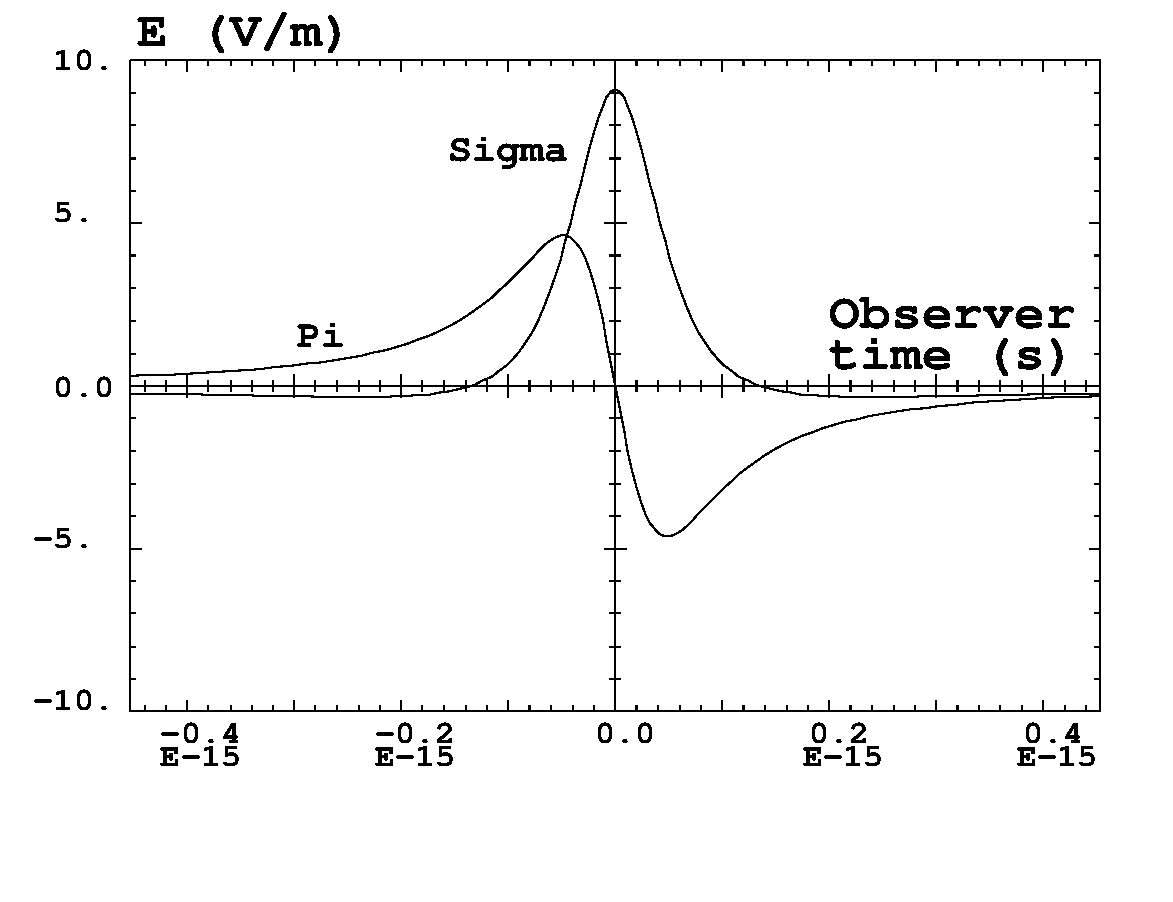
\includegraphics[width=7.9cm]{FigSRE.eps}
        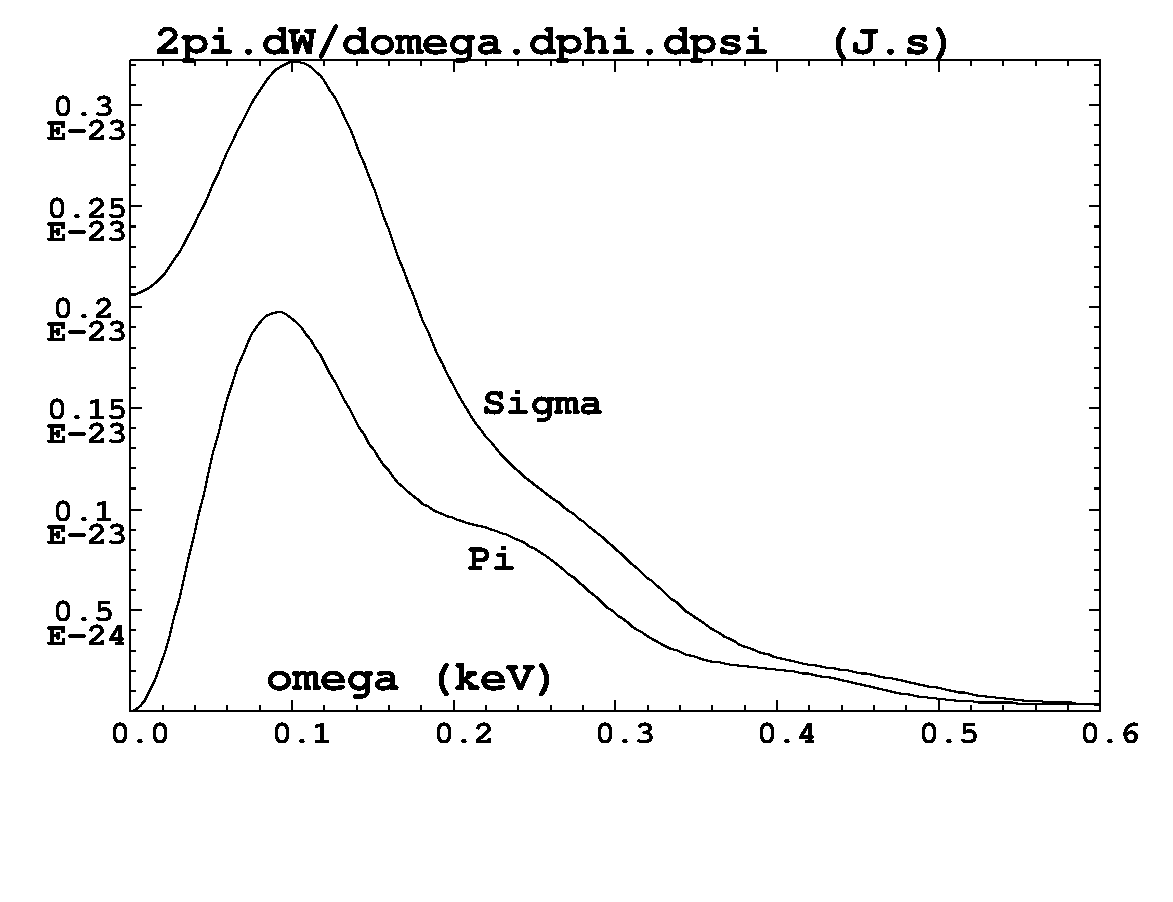
\includegraphics[width=7.9cm]{FigSRP.eps}
      }
  \end{center}
  \vspace{-1.5cm}
  \hangcaption{ \label{FigSREP} 
  {\it Left}~: typical shapes of the $\Ecal_{\sigma}(t)$  and $\Ecal_{\pi}(t)$ components of the electric field impulse 
(eq.~\ref{eqN4.1}) emitted by a 2.5~GeV electron on a $\rho=53.6$~m circular trajectory in a $l=20$~cm-long dipole, 
as observed in the direction of the centre of the dipole, $\phi=0$, 
$\gamma \psi=5$ (observation distance $r=10$~m). 
{\it Right}~: the related spectral angular densities  
$\partial^3 W_{\sigma,\, \pi}/\partial\phi\, \partial\psi\, \partial\omega$ (eq.~\ref{eqN4.10}). After Ref.~\cite{PALowFreq}. 
   }
\end{figure}

\noindent As an illustration, Fig.~\ref{FigSREP} has been produced using \zpop, 
it shows the typical shape of the electric field impulse at the observer, with central peak  width~\cite{PALowFreq}  
$$  2 \, \tau_c = 2 \, \dfrac{2\rho }{ 3\gamma^3~c} \, (1 +\gamma^2\psi^2)^{3/2}$$


\section*{Computation of $\vec{n} - \vec{\beta}$ and $1 - \vec{n} \cdot \vec{\beta}$}
 
Owing to computer precision the crude computation of $\vec{n} -
\vec{\beta}$ and $ 1 -\vec{n}\cdot \vec{\beta}$ may lead to
$$
	\vec{n} - \vec{\beta} = 0 \text{ and } 1 - \vec{n}\cdot \vec{\beta} = 0
$$
since the preferred direction of observation is generally almost parallel to
$\vec{\beta}$ (in that case, parallel in the sense of computer precision), while $\beta
\approx$ 1 as soon as particle energies of a few hundred times the rest mass are
concerned.

\noindent It is therefore necessary to express $\vec{n} - \vec{\beta}$ 
and $1 -\vec{n} \cdot
\vec{\beta}$ in an adequate  form for achieving accurate software  computation.

\noindent The expression for $\vec{n}$ is

\begin{multline} \label{eqN4.5}
	\vec{n} = (n_x, n_y, n_z) = (\cos \psi\,\cos \phi, \cos \psi \,\sin 
		\phi, \sin \psi)  \\
	= \left[1 - 2 (\sin^2\phi/2 + \sin^2 \psi/2) + 4 \sin^2\phi/2 \sin^2\psi/2, 
		\sin \phi (1 - 2\sin^2\psi/2), \sin \psi \right]
\end{multline}
%
where $\phi$ and $\psi$ are the observation angles, given by 

\begin{equation}
	\phi = \text{Atg} \left( \dfrac{r_y}{ r_x}\right)
	\text{ and }  \psi = \text{Atg}\left( \dfrac{r_z}{\sqrt{r_x^2 + r_y^2}}\right) \label{eqN4.6}
\end{equation} %\label{eqN4.6}
%
with $\vec{r} = (r_x, r_y, r_z)$, while $\vec{\beta}$ can be written under the form

\begin{multline} \label{eqN4.7}
	\vec{\beta} = (\beta_x, \beta_y, \beta_z) = 
		\left[ \sqrt{(\beta^2 - \beta^2_y - \beta_z^2)},\beta_y, \beta_z 
		\right] \\
	= \left[ \sqrt{(1 - 1/\gamma^2 - \beta_y^2 - \beta_z^2)}, \beta_y, 
		\beta_z \right] = (1 - a/2 + a^2/8 - a^3/16 +...,\beta_y, \beta_z) 
\end{multline}
%
where $a = 1/ \gamma^2 + \beta^2_y + \beta^2_z$. This leads to

\begin{gather*}
	n_x = 1 - \varepsilon_x 
		\text{ and } \beta_x = 1 - \xi_x  \\
\intertext{with}
\varepsilon_x = 2 (\sin^2\phi/2 + \sin^2\psi/2) - 4 \sin^2\phi/2  \sin^2\psi/2 \\
\intertext{and}
\xi_x = a/2 - a^2/8 + a^3/16 +...
\end{gather*}

\noindent All this provides, on the one hand, 

\begin{equation}
\vec{n} - \vec{\beta} = (-\varepsilon_x + \xi_x, n_y - \beta_y, n_z - \beta_z)~,  \label{eqN4.8}
\end{equation}   %\label{eqN4.8}
%
whose components are combinations of terms of the same order of magnitude
($\varepsilon_x$ and $\xi_x \sim 1/\gamma^2$ while $n_y, \beta_y, n_z$ and $\beta_z \sim
1/\gamma$) and, on the other hand,

\begin{equation}
1 - \vec{n} \cdot \vec{\beta} = \varepsilon_x + \xi_x - n_y\beta_y - n_z\beta_z -  \label{eqN4.9}
\varepsilon_x\xi_x~,
\end{equation}  %\label{eqN4.9}
%
that combines terms of the same order of magnitude ($\varepsilon_x, \xi_x, n_y\beta_y$
and $n_z\beta_z \sim 1/\gamma^2$), plus $\varepsilon_x\beta_x \sim 1/\gamma^4$.

\noindent The precision of these expressions is
directly related to the order at which the series

$$
	\xi_x = a/2 - a^2/8 + a^3/16 +... \qquad(a = 1/\gamma^2 + \beta_y^2 +\beta^2_z)
	$$
is pushed, however the convergence is   fast since $ a \sim 1/\gamma^2 \ll 1$ in situations of concern. 

\subsubsection{Calculation of the Fourier Transform of the Electric Field}\label{secN4.2}

The Fourier transforms
$$
	FT_\omega  [ \vec \Ecal (\tau)] = \int \vec \Ecal  (\tau) e^{-i\omega\tau} d\tau~$$
of the $\sigma$ and $\pi$ electric field components provide the spectral angular
 energy density 

\begin{equation}
     \dfrac{\partial^3 W}{\partial\phi\, \partial\psi\, \partial\omega} 
		= \dfrac{ r^2 }{ \mu_0 c}
            \left| FT_\omega \left(\vec  \Ecal (\tau) \right)  \right|^2  \label{eqN4.10}
\end{equation}  %\label{eqN4.10}
%
Fig.~\ref{FigSREP}-right gives a typical example in the case of a short magnet. 
These  Fourier transforms are computed without resorting to  FFT techniques, namely from 

\begin{equation}
	FT_\omega \left[ \vec \Ecal  (\tau) \right] 
		\approx \sum \vec \Ecal (\tau_k)\, e^{-i\omega\tau_k} \, \Delta\tau_k  \label{eqN4.11}
\end{equation}    %\label{eqN4.11}
%
for two reasons. On the one hand, the number of integration steps $\Delta s$ that define the
trajectory (eqs.~\ref{eq2-2-4}), is arbitrary and therefore in general not of order $2^n$.
On the other hand, the integration step defines a constant time differential element 
$\Delta t_k = \Delta s/ \beta c$ which results in the observer differential time 
element $ \Delta \tau_k$, which is
also the differential element of the Fourier transform, being non-constant, since both
are related by eq.~\ref{eqN4.2} in which $\vec{\beta}$ and $\vec{n}$ 
vary as a function of the  integration step number~$k$.

\medskip

\noindent An additional issue is that  $ \Delta \tau_k$ may reach drastically small values 
in the region of the central peak of the electric impulse emitted in 
a dipole, \ie, $1 - \vec{n}(t) \cdot \vec{\beta} (t) \to
1/2\gamma^2$, whereas the total integrated time $\sum_{k=1}^{N} \Delta \tau_k$ may be several
orders of magnitude larger. In terms of the physical phenomenon, the total duration of the electric 
field impulse as seen by the observer corresponds to the time delay $ \sum_{k=1}^{N} \Delta \tau_k$
that separates photons emitted at the
entrance of the magnet from photons emitted at the exit, but the significant  part of it
(in terms of energy density) which can be represented by the width 
$ 2\, \tau_c = 2\, \dfrac{2\rho }{ 3\gamma^3~c} (1 +\gamma^2\psi^2)^{3/2}$ of the  
radiation peak, is a very small fraction of $ \sum_{k=1}^{N} \Delta \tau_k$.

\noindent The consequence is that, again in relation to computer precision, the
differential  element $\Delta \tau_k$ involved in the computation of 
eq.~\ref{eqN4.11} cannot be derived from such relation as 
 $\Delta\tau_k = \sum_{k=1}^{n} \Delta\tau_k - \sum_{k=1}^{n-1} \Delta \tau_k$ 
but instead must be stored as is,  in the course of the ray-tracing process, for 
subsequent data treatment. 


%%%%%%%%%%%%%%%%% previous part 4 %%%%%%%%%%%%%%%%%%%%%%%%%
\clearemptydoublepage

\section{DESCRIPTION OF THE AVAILABLE PROCEDURES} \label{sec4}

\subsection{Introduction} \label{4.1} 


This chapter gives an inventory of the  procedures available in \zgoubi, 
 their associated ``keyword'',  and a brief  description  of the way  they function. 

\medskip 
 
\noindent The chapter  has been 
split into several sections. Sections~\ref{sec4.2} to~\ref{sec4.5} explain the 
underlying content - physics and numerical  methods -  behind the  keywords, they are organized by topics~: 

- How to defined an object (a set of initial coordinates), 

- Available options, 

- Optical elements and procedures,

- Output procedures.

\medskip 
 
\noindent Section~\ref{sec4.6} addresses further a series of 
functionalities that may be accessed  by means of special input data or flags. 


%%%%%%%%%%%%%%%%% previous part 4 %%%%%%%%%%%%%%%%%%%%%%%%%
\clearemptydoublepage


\subsection{Definition of an Object} \label{sec4.2}

The description of the object, \emph{i.e.}, initial coordinates of the ensemble of  
particles, must be the first procedure in the  \zgoubi\ input data file, zgoubi.dat.  

 \bigskip

\noindent Several types of automatically generated objects are available, 
they are described in the following pages and include, 

- non-random object, with various distributions~: individual particles, grids, object for \textsl{MATRIX}, etc.

- Monte Carlo distribution, with various distributions as well~: 6-D window, ellipsoids, etc.

 \bigskip

\noindent A recurrent quantity appearing in these procedures is \IMAX, the  number of particles to be ray-traced. 
The maximum value allowed for \IMAX\  can be changed at leisure in the include file \texttt{'MAXTRA.H'} 
where it is defined (that requires re-compiling \zgoubi). 







\clearpage

\subsubsection*{MCOBJET~:  \MCOBJETTitl} \label{MCOBJET} \index{MCOBJET|textbf}
\index{Monte Carlo}\index{negative charge}\index{negative momentum} 
\medskip 



\noindent \textsl{MCOBJET} generates a set of \IMAX\ random 6-D initial
conditions (the maximum value for \IMAX\ is defined in the include file \texttt{'MAXTRA.H'}). 
It can be used in conjunction with the keyword \textsl{REBELOTE\index{REBELOTE}}
which   either allows generating an arbitrarily high number of initial conditions, or, in the 
hypothesis of a periodic structure, 
 allows multi-turn tracking \index{multi-turn tracking} with initial conditions at pass number $\IPASS$ 
identified with conditions at end of pass number $\IPASS-1$.  

 \bigskip

\noindent The first datum in \textsl{MCOBJET}  is the reference rigidity (a negative value is 
allowed)  \index{reference rigidity} 
$$ \BORO = \dfrac{p_0 }{ q} \text{ (kG.cm)} $$\index{BORO@{\BORO}|textbf}

\noindent Depending on the value of the next datum, \textsl{KOBJ}, the 
\IMAX\index{IMAX@{\IMAX}|textbf} particles have their initial random 
conditions $ Y$, $T$, $Z$, $P$, $X$ and $ D $ (relative rigidity, $B\rho/\BORO$)  generated 
on 3~different types of supports, as described below. 

\noindent Next come the data
$$\KY, \KT, \KZ, \KP, \KX, \KD$$  %%%%%%%%% $$ KH,\quad KV,\quad KP $$
that specify the type of probability density for the 6~coordinates. 

\noindent $\KY$, $\KT$, $\KZ$, $\KP$, $\KX$ can take the following values~:
\begin{enumerate}
\item uniform density, $p(x) =1/2\delta x$ if  $-\delta x \leq x \leq \delta x$, $p(x) = 0$ elsewhere,
\item Gaussian density, $p(x) = \dfrac{1}{\delta x \sqrt{2\pi}} 
	e^{- \dfrac{x^2}{2 \delta x^2}}$,
\item parabolic density, $p(x) = \dfrac{3}{4 \delta x} 
	(1- \dfrac{x^2}{\delta x^2})$ if $-\delta x \leq x \leq \delta x$, $p(x) = 0$ elsewhere.
\end{enumerate}

\noindent $\KD$ can take the following values~:
\begin{enumerate}
\item uniform density, $p(D) =1/2\delta \! D$ if  $-\delta \! D \leq D \leq \delta \! D$, $p(D) = 0$ elsewhere,
\item exponential density, $p(D) = N_0 \exp (C_0 + C_1 l + C_2 l^2 + C_3 l^3)$
	with $0 \leq l \leq 1$ and $-\delta D \leq D \leq \delta D$,
\item $p(D)$ is determined by a kinematic relation, namely, with $T=$ 
horizontal angle, $D= \delta D \ast T$.
\end{enumerate}

\noindent Next come the central values for the random sorting, 
$$    Y_0,\quad    T_0,\quad    Z_0,\quad P_0,\quad  X_0, \quad D_0 $$
%
namely, the probability density laws $p(x)$ ($x= Y, T, Z, P$ or $X$) 
and $p(D)$ described above apply to the variables $x-x_0$
( $\equiv Y- Y_0$, $T-T_0$, ...) and $D- D_0$ respectively. Negative 
value for $D_0$ is allowed (see section~\ref{sec4.6.7}, page~\pageref{sec4.6.7}).
 \bigskip

\noindent\textbf{KOBJ  =  1}~: Random  generation of \IMAX\ particles  
in a hyper-window with widths
(namely the half-extent for uniform or parabolic distributions ($KY, 
KT, ... =1$ or 3), and  the r.m.s.~width for Gaussian distributions ($KY, 
KT, ... =2$))
$$   \delta Y,\quad   \delta T,\quad   \delta Z,\quad   \delta P,\quad   \delta X,\quad  \delta D $$

\noindent Then follow the cut-off values, in units of the 
r.m.s.~widths $\delta Y$, $\delta T$, ... (used only for  Gaussian distributions,  
$KY, KT, ... =2$)
$$
	N_{\delta Y},\quad N_{\delta T},\quad N_{\delta Z},\quad N_{\delta P},\quad N_{\delta X},\quad N_{\delta D}
$$	 
\noindent The last data are the parameters 

$$ N_0,\quad C_0,\quad C_1,\quad C_2,\quad C_3 $$ 
%
 needed for generation of the $ D $ coordinate upon option
 $ KD  =  2$ (unused if $ KD = 1,~3$) and a set of three integer seeds for initialization of random sequences,
 
 $$ IR1,\quad   IR2, \quad  IR3 \quad \text{(all $\simeq 10^6 $)}$$
%

\medskip

\noindent All particles generated by \textsl{MCOBJET\index{MCOBJET}}  are tagged \index{tag, tag character} 
with a (non-S) character, for further statistic purposes 
(\emph{e.g.}, with \textsl{HISTO\index{HISTO}}, \textsl{MCDESINT\index{MCDESINT}}).  
\medskip

\noindent\textbf{KOBJ  =  2}~: Random  generation of 
$\IMAX =  IY \ast   IT  \ast IZ \ast  IP  \ast  IX  \ast  ID $ particles    
 on a  hyper-grid.  The input data are the number of bars    in 
each coordinate

 \begin{gather*}
	 IY,\quad IT,\quad IZ,\quad IP,\quad IX, \quad ID \\
%
\intertext{the spacing of the bars} 
	PY,\quad PT,\quad PZ,\quad PP,\quad PX, \quad PD \\
%
\intertext{the width of each bar} 
	\delta Y,\quad \delta T,\quad \delta Z,\quad \delta P,\quad \delta X,\quad \delta D  \\
%
\intertext{the cut-offs, used with Gaussian densities (in units of the r.m.s. widths)}
	N_{\delta Y},\quad N_{\delta T},\quad N_{\delta Z},\quad N_{\delta P},\quad N_{\delta X},\quad N_{\delta D}
 \end{gather*}
%\medskip

\noindent This is illustrated in Fig.~\ref{fig5}.

\medskip

\noindent The last two sets of data in this option are the parameters 

 \begin{gather*}
	N_0,\quad C_0,\quad C_1,\quad C_2,\quad C_3 
 \end{gather*}
%
 needed for generation of the $ D $ coordinate upon option \mbox{KD=  2}  
(unused if \mbox{KD= 1, 3}) and a set of three integer seeds for initialization 
of random sequences, $ IR1$,   $ IR2$,   and $ IR3$ (all $\simeq 10^6 $).

%\medskip

\noindent All particles generated by \textsl{MCOBJET\index{MCOBJET}}  are tagged with \index{tag, tag character} 
a (non-S) character, for further statistic purposes (see \textsl{HISTO\index{HISTO} \textrm{and}  
MCDESINT\index{MCDESINT}}).  

\medskip

\noindent\textbf{KOBJ  = 3~:} Distribution of \IMAX\ particles inside a
6-D ellipsoid defined by the three sets of data (one set per 
 2-D phase-space)

$$
\begin{array}{*{4}{r<{,}}r}
 \alpha_ Y  &   \beta_ Y  
            &  \dfrac{ \varepsilon_Y}{\pi} 
            &  N_{\varepsilon_ Y}  ~~[
            & N'_{\varepsilon_ Y}, \text{ if } N_{\varepsilon_ Y} < 0] \\
\alpha_ Z   &  \beta_ Z  
            &  \dfrac{ \varepsilon_Z }{ \pi} 
            & N_{\varepsilon_ Z} ~~[
            & N'_{\varepsilon_ Z}, \text{ if } N_{\varepsilon_ Z} < 0] \\
\alpha_ X   & \beta_ X 
            &  \dfrac{\varepsilon_X }{ \pi} 
            & N_{\varepsilon_ X} ~~[
            & N'_{\varepsilon_ X}, \text{ if } N_{\varepsilon_ X} < 0] 
\end{array}           
$$            
%
where $\alpha$, $\beta$ are the ellipse parameters and $\varepsilon/ 
\pi$ the \rms\ emittance, corresponding to an elliptical  frontier 
$\dfrac{1 + \alpha^2_Y}{\beta_Y} Y^2 + 2 \alpha_Y YT + \beta_Y T^2 = 
\varepsilon_Y / \pi$ (\id\ for the ($Z, P$) 
or ($X, D$) planes). $N_{\varepsilon_ Y}$, $N_{\varepsilon_ Z}$ and 
$N_{\varepsilon_ X}$ are the sorting cut-offs (used only for Gaussian 
distributions, $KY, KT, ...=2$).

\noindent The sorting is uniform in surface (for $KY=1$ or $KZ=1$ 
or $KX=1$) or Gaussian ($KY=2$ or $KZ=2$), and so on, as described 
above. A uniform sorting has the ellipse above for support. A 
Gaussian sorting has the ellipse above for r.m.s.~frontier, leading 
to $\sigma_Y = \sqrt {\beta_Y \varepsilon_Y / \pi}$, 
$\sigma_T = \sqrt {\dfrac{(1+\alpha_Y^2)}{\beta_Y} \varepsilon_Y / \pi}$, 
and similar relations for $\sigma_Z$, $\sigma_P, \sigma_X$, $\sigma_D$.

\noindent If $N_\varepsilon$ is negative, thus the sorting fills the 
elliptical ring that extends from $\left| N_\varepsilon \right|$ to 
$N'_\varepsilon$ (rather than the inner region determined by the $N_\varepsilon$ 
cut-off as discussed above).


\vfill
%%%%%%%%%%%%%%figure %%%%%%%%%%%%%
 \begin{figure}[H]
  % \vspace*{19 truecm}
\centerline{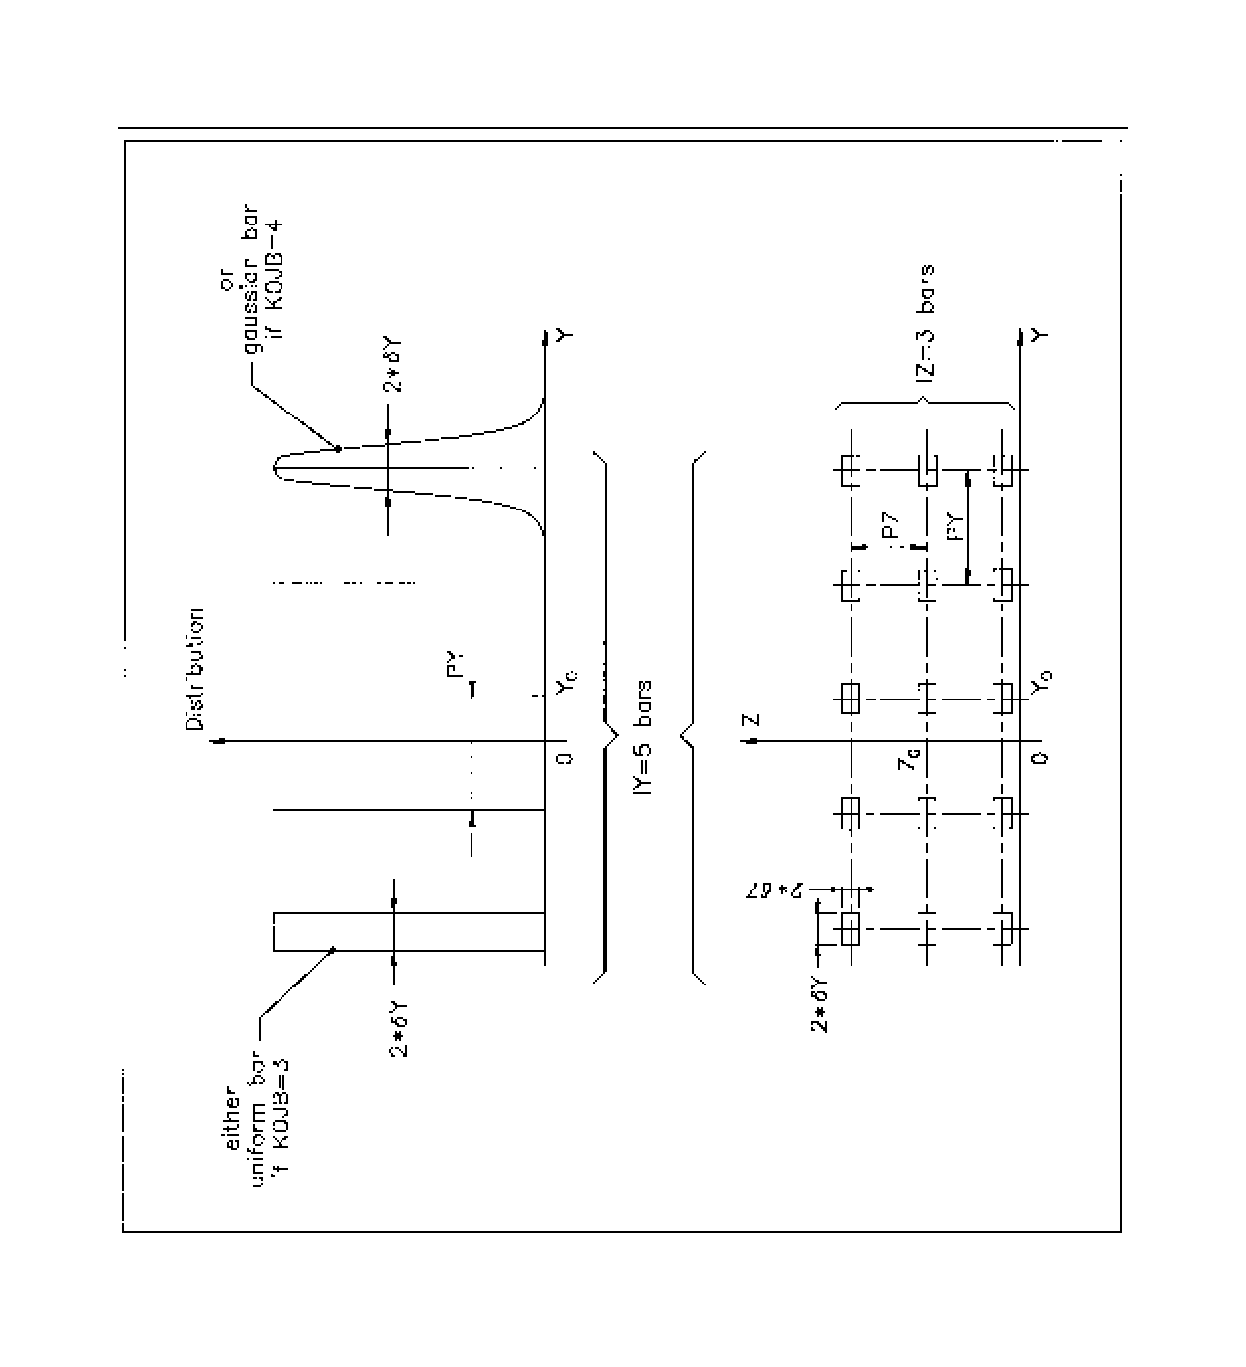
\includegraphics[width=15cm,angle=-90]{Fig5.ps}}  %% now 6
	\hangcaption[Fig5]{\label{fig5}A scheme of  input parameters to \textsl{MCOBJET} when \KOBJ = 2. \\
   Top~: Possible  distributions  of the $ Y $ coordinate. \\ 
Bottom~: A 2-D grid in ($ Y, Z $) space.} 
 \end{figure}
 \vfill 





\clearpage

 
\subsubsection*{OBJET~:   \OBJETTitl} \label{OBJET} \index{OBJET|textbf}
\medskip 
\index{negative charge}\index{negative momentum}



\textsl{OBJET} is dedicated to the construction of sets of  initial coordinates, in several ways.  
\medskip

\noindent The first datum is the reference rigidity (a negative value is allowed) \index{reference rigidity} 
 
$$ \BORO = \dfrac{p_0 }{ q}  $$\index{BORO@{\BORO}|textbf}

\noindent At the object, the beam is defined by a set of \IMAX\ particles 
(the maximum value for \IMAX\ is defined in the include file \texttt{'MAXTRA.H'}) with 
the initial conditions ($ Y$, $T$, $Z$, $P$, $X$, $D$)  with $ D =B\rho/\BORO$ 
 the relative rigidity. 

\noindent Depending on the value of the next datum \textsl{KOBJ}, these initial
conditions may be generated   in eight different ways~:   
\bigskip

\noindent\textbf{KOBJ  =  1}~:  Defines a grid in the $ Y$, $T$, $Z$, $P$, $X$, $D$
 space. One gives the number of points desired 
% \begin{gather*}
$$	 IY,\quad IT,\quad IZ,\quad IP, \quad IX, \quad ID\\$$
with  $ IY\leq n_Y \ldots ID\leq n_D$ such that $ n_Y \times n_T \times ... \times n_D \leq \textsl{max}(\IMAX)$. 
 One defines the sampling range in each coordinate
$$	 PY,\quad PT,\quad PZ,\quad PP,\quad PX, \quad PD  $$
% \end{gather*}


\noindent\zgou\  then generates 
$ \IMAX = IY  \ast  IT  \ast  IZ \ast   IP \ast IX \ast  ID $ particles with  initial coordinates 

$$
  \begin{array}{*{5}{r<{,}}}
	  0  &  \pm PY &   \pm 2  \ast   PY & \ldots & \pm IY/2  \ast   PY \\
	  0  &  \pm PT &   \pm 2 \ast   PT  & \ldots &  \pm IT/2  \ast   PT \\
	  0  &  \pm PZ &   \pm 2 \ast  PZ   & \ldots &  \pm IZ/2 \ast PZ \\
	  0  &  \pm PP &   \pm 2  \ast PP  & \ldots  &  \pm IP/2  \ast  PP \\
	  0  &  \pm PX &   \pm 2  \ast  PX & \ldots  &  \pm IX/2 \ast   PX \\
 	  0  &  \pm PD &   \pm 2  \ast  PD & \ldots  &  \pm ID/2 \ast   PD 
 \end{array}
 $$

\medskip

\noindent In this option relative rigidities  will be classified automatically in view of possible 
further  use of $\IMAGES[Z]$\index{IMAGES} for momentum analysis and image formation. 


\noindent The particles are tagged with an index \textsl{IREP} possibly
indicating a symmetry \index{tag, symmetry index} with respect to the ($ X$,$Y$) plane, as explained in option 
\mbox{\KOBJ= 3}. If two trajectories have mid-plane symmetry, only one  will be 
ray-traced, while the other will be deduced using the mid-plane 
symmetries. This is done for the purpose of saving computing time. It may 
be incompatible with the use of some procedures (\emph{e.g.}~\textsl{MCDESINT\index{MCDESINT}}, which 
involves random processes). 

\noindent The last datum is a reference in each coordinate, $\YR,\TR,\ZR,\PR,\XR,\DR$. 
For instance the reference rigidity is $ DR \ast$ \BORO, resulting 
 in the rigidity of a particle of initial condition $ I\ast PD $ to be 
$ (DR+I\ast PD)\ast \BORO$. 

\bigskip

\noindent\textbf{KOBJ = 1.01}: Same as \KOBJ = 1    except for the $ Z $
symmetry.  The initial $ Z $ and $ P $ conditions are the following 

$$
  \begin{array}{*{5}{r<{,}}}
	  0  &  PZ &   2  \ast   PZ & \ldots & (IZ-1)   \ast   PZ \\
	  0  &  PP &   2 \ast   PP  & \ldots & (IP-1)   \ast   PP 
  \end{array}
 $$


\noindent This object results in shorter outputs/CPU-time when studying problems with $Z $ symmetry.  

\bigskip

\noindent\textbf{KOBJ = 2~:}  Next data~: \IMAX\index{IMAX@{\IMAX}|textbf},  
\IDMAX\index{IDMAX@{\IDMAX}|textbf}. Initial coordinates
are entered explicitly for each 
trajectory.  \IMAX\  is the total number of particles.  
These may be classified in groups of equal number for each value of momentum, in order to 
fulfill the requirements of image calculations by \textsl{IMAGES$[\textsl{Z}]$\index{IMAGES}}. 
 \IDMAX\index{IDMAX@{\IDMAX}} is the 
number of groups of momenta.  The  following initial 
conditions defining a particle are specified for each one of the \IMAX\  
 particles
 $$ Y,\quad T,\quad Z,\quad P, \quad X, \quad D,\quad ^\prime A^\prime $$
%
 where $ D\ast \BORO$ is the rigidity (negative value   
 allowed) and $ ^\prime A^\prime $ is a
(arbitrary) tagging character.  \index{tag, tag character} 


\smallskip

\noindent The last record \IEX\index{IEX@{\IEX}|textbf} (I=1, \IMAX)  contains 
\IMAX\  times either the character  ``1'' to indicates that the particle has to  be
tracked,  or ``-9''  to indicates that the particle should not be tracked.  

\smallskip

\noindent This option \mbox{\KOBJ= 2}   may be be useful for the definition of objects including kinematic  effects.  



\bigskip

\noindent\textbf{KOBJ = 2.01}: Same as \KOBJ = 2    except for the units, meter and radian in that case. 




\bigskip


%\newpage 


\noindent\textbf{KOBJ $= 3$~:} This option allows the reading of initial conditions from an
external input file \textsl{FNAME}.  

\noindent The next three data lines are~: 

\smallskip 

\ITone, \ITtwo, \ITStep

\IPone, \IPtwo, \IPStep

\YF, \TF, \ZF, \PF, \SF, \DPF, \TiF, \TAG      \index{tag, tag character} 

\YR, \TR, \ZR, \PR, \SR, \DPR, \TiR

\textsl{InitC}

\smallskip 

\noindent followed by the storage file name \textsl{FNAME}. 

\smallskip 

\noindent \ITone, \ITtwo, ITStep\ cause the code to read coordinates of particles number \ITone\ through  \ITtwo\ by step \ITStep. 

\smallskip 

\noindent \IPone, \IPtwo, \IPStep\  cause the code to read coordinates belonging in the  passes range   
 \IPone\ through  \IPtwo,  step \IPStep. 


\smallskip 

\noindent \YF, \TF, \ZF, \PF, \SF, \DPF, \TiF\ are scaling factors whereas 
 \YR, \TR, \ZR, \PR, \SR, \DPR, \TiR\ are  references added to the  values of respectively Y, T, Z, P, S, DP as read 
in  file \textsl{FNAME}, 
 so that any coordinate $C=Y,T,Z...$ is changed into CF*C + CR. 
In addition a flag character TAG allows retaining only particles with identical tagging letter LET, unless 
TAG='*' in which case it has no selection effect - for instance TAG='S' can be used to retain only secondary 
particles following in-flight decay simulations. 

\smallskip 

\noindent 
If \mbox{InitC$=1$} ray-tracing starts from the current coordinates$ F(J,I)$, \\
if \mbox{InitC$=0$}  ray-tracing starts from the initial coordinates $ FO(J,I)$,  as read from file \textsl{FNAME}. 

\smallskip 


\noindent The  file \textsl{FNAME} must be formatted in the appropriate manner. 
The following \FORTRAN\ sequence is an instance, details and possible updates are to be found in the source  
file \texttt{'obj3.f'}~:  
\begin{alltt}
\footnotesize

         OPEN (UNIT = NL, FILE = FNAME, STATUS = `OLD')
	 DO I = 1, IMAX
	    READ (NL,100) LET (I), IEX(I), (FO(J,I),J=1,6), (F(J,I),J=1,6), I, IREP(I),
     >      LET(I),IEX(I),-1.D0+FO(1,I),(FO(J,I),J=2,MXJ),
     >      -1.D0+F(1,I),F(2,I),F(3,I),
     >      (F(J,I),J=4,MXJ),ENEKI,
     >      ID,I,IREP(I), SORT(I),D,D,D,D,RET(I),DPR(I),
     >      D, D, D, BORO, IPASS, KLEY,LBL1,LBL2,NOEL
 100        FORMAT(1X,
C1   LET(IT),KEX,   1.D0-FO(1,IT),(FO(J,IT),J=2,MXJ),
     1           A1,1X,I2,1P,7E16.8,
C2   1.D0-F(1,IT),(FO(J,IT),J=2,MXJ),
     2         /,3E24.16,
C3   Z,P*1.D3,SAR,     TAR,     DS,
     3         /,4E24.16,E16.8,
C4   KART,  IT,IREP(IT),SORT(IT),X, BX,BY,BZ, RET(IT), DPR(IT),
     4         /,I1,2I6,7E16.8,
C5        EX,EY,EZ, BORO,  IPASS,  KLEY,  (LABEL(NOEL,I),I=1,2),NOEL
     5  /,4E16.8,          I6,1X,  A8,1X,  2A10,                I5)
  ENDDO
\end{alltt} 

\noindent where the meaning of the parameters (apart from D=dummy real, ID=dummy integer) is the following   
\medskip
 
\begin{tabular}{>{\sl}l!{:}p{10cm}}
LET(I) & one-character string (for tagging)  \\  \index{tag, tag character} 
 IEX(I)\index{IEX@{\IEX}} &  flag, see \KOBJ = 2 and page~\pageref{sec4.6.6} \\
 FO(1-6,I) &  coordinates $ D$, $Y$, $T$, $Z$, $P $ and path length of 
particle number $I$,  at the origin. $ D\ast \BORO $ = rigidity \\
F(1-6,I) & id, at the current position.
\end{tabular}
\medskip

\noindent\textsl{IREP}   is an index which indicates a symmetry with
respect to the median plane.  For instance, if $ Z(I+1)=-Z(I), $ then normally 
\textsl{IREP}$(I+1)=$ \textsl{IREP}$(I)$.
Consequently the coordinates of particle $ I+1 $ will not be obtained from 
ray-tracing but instead deduced  from those of 
particle $ I $ by simple symmetry.  This saves on computing time.

\bigskip

\noindent\KOBJ $= 3 $    can be used for reading files filled by \textsl{FAISCNL}, \textsl{FAISTORE}.\\
If more than \IMAX\ particles are to be read from a file, use  \textsl{REBELOTE\index{REBELOTE}}.   

\bigskip

\noindent Note~: In this option, one has to make sure that input data do not conflict with possible use of 
the keyword \textsl{PARTICUL} that  assigns   mass and charge.

\bigskip

\noindent\textbf{KOBJ = 3.01:} Same as \textbf{KOBJ = 3}, except for the formatting of trajectory coordinate 
data in  \textsl{FNAME}, namely, according to the following \FORTRAN\ sequence 
\begin{alltt}
\footnotesize
         OPEN (UNIT = NL, FILE = FNAME, STATUS = `OLD')
    1    CONTINUE
         READ (NL,*,END=10,ERR=99) Y, T, Z, P, S, D
         GOTO 1
   10    CALL ENDFIL
   99    CALL ERREAD
\end{alltt} 

\bigskip

\noindent\textbf{KOBJ = 3.02:} As for \textbf{KOBJ=3.01}, except for the different format
\begin{alltt}
         READ(NL,*) X,Y,Z,PX,PY,PZ
\end{alltt}
where \texttt{PX}, \texttt{PY}, and \texttt{PZ}, are the momenta in
MeV/$c$.  Note that DPR will be ignored in this case.

\bigskip

\noindent\textbf{KOBJ = 3.03:} As for \textbf{KOBJ=3.01}, except for the different format~: 
\begin{alltt}
         READ(NL,*) DP,Y,T,Z,P,S,TIME,MASS,CHARGE
\end{alltt}
where \texttt{MASS} is the mass in MeV/$c$ and \texttt{CHARGE} is the
charge in units of the elementary charge.  

%In this case, particles will not have the reference
%charge and \textsl{PARTICUL} will not assign a mass or charge.


\bigskip

\noindent \textbf{Note~:}  For details and possible updates in the formatted read of concern in the \FORTRAN, 
regarding options 3.01-3.03, see the source file \texttt{'obj3.f'}.


\bigskip


\noindent\textbf{KOBJ = 5~:} Mostly dedicated to the calculation of first order
transfer matrix and various other  optical parameters, 
 using for instance \textsl{MATRIX\index{MATRIX}} or \textsl{TWISS\index{TWISS}}.  
The input data are the coordinate sampling 
\smallskip
$$ PY,\quad PT,\quad PZ,\quad PP, \quad PX, \quad PD $$

\noindent The code generates  11 particles,  with initial coordinates 
$$ 0,\quad \pm PY,\quad \pm PT,\quad \pm PZ,\quad \pm PP, \quad \pm PX, \quad \pm PD $$

\noindent These values should be small enough, so that the paraxial ray
approximation be valid. 
 The last data line gives  the reference 
$$YR, \quad TR, \quad ZR, \quad PR, \quad XR, \quad DR $$
(with $ DR\ast \BORO$  the reference rigidity - negative value allowed), which adds to the previous 
coordinate  values.


\bigskip

\noindent\textbf{KOBJ = 5.01:} Same as \textsl{KOBJ = 5}, except for an additional data line giving 
initial beam ellipse parameters and  dispersions,  
$\alpha_Y, \beta_Y$, $\alpha_Z, \beta_Z$, $\alpha_X, \beta_X$, $D_Y$ , $D'_Y$ , $D_Z$ , $D'_Z$,  
 for further transport of these using \textsl{MATRIX}, or for  possible use by the \textsl{FIT[2]}\index{FIT}\index{FIT2} procedure. 

\bigskip

\noindent\textbf{KOBJ = 5.NN:} Like \textsl{KOBJ = 5}, except for  $NN = 02 - 99$ references needed in this case 
(thus \textsl{NN-1} additional input data lines), rather than just one. 
Zgoubi will generate  \textsl{NN} sets of 11 particles with initial  coordinates in each set taken \wrt\ one 
of the  \textsl{NN} references. 

\medskip 

\noindent A subsequent use of \textsl{MATRIX}  would then cause the computation of \textsl{NN} transport matrices. 


\bigskip

\noindent\textbf{KOBJ = 6:}  Mostly dedicated to the calculation of first, second
and other higher order transfer coefficients and various other  optical parameters, 
using for instance \textsl{MATRIX\index{MATRIX}}. 
The input data are the coordinate sampling (normally taken paraxial)  

$$ PY,\quad PT,\quad PZ,\quad PP, \quad PX, \quad PD $$
 
 \noindent to allow the building up of an object containing 61 particles (note~: their coordinates can be 
checked by printing out into zgoubi.res using \textsl{FAISCEAU}), whereas   a last data line gives  the reference 
$$YR, \quad TR, \quad ZR, \quad PR, \quad XR, \quad DR $$
(with $ DR\ast \BORO$  the reference rigidity - negative value allowed), which adds to the previous 
 coordinate values.


\bigskip


\noindent\textbf{KOBJ = 7~:} Object with kinematics 

\noindent The data and functioning are the same as for \mbox{\KOBJ= 1}, except for the 
following  
\begin{itemize}
\item[$\bullet$]  $ ID $ is not used,  
\item[$\bullet$]  $ PD $ is the kinematic coefficient, such that for particle
number $ I$,  the initial relative rigidity $ D_I $ is calculated from the initial angle 
$T_I $ following
$$ D_I = DR+ PD \ast  T_I $$
 while $ T_I $ is in the range
$$ 0,\quad \pm PT,\quad \pm 2\ast PT,\quad \ldots,\quad \pm IT/2\ast PT $$
 as stated under \KOBJ = 1
\end{itemize}

\bigskip


\noindent\textbf{KOBJ = 8~:} Generation of phase-space coordinates on ellipses. 

\noindent The ellipses are defined by  the three sets of data (one set per 
  ellipse) 

$$
\begin{array}{*{2}{r<{,}}r}
 \alpha_ Y  &   \beta_ Y  
            &  \varepsilon_Y / \pi \\
\alpha_ Z   &  \beta_ Z  
            &  \varepsilon_Z / \pi \\
\alpha_ X   & \beta_ X 
            &  \varepsilon_X / \pi 
\end{array}           
$$            
%
where $\alpha$, $\beta$ are the ellipse parameters  and $\varepsilon/$ is the 
ellipse surface, corresponding to an ellipse with equation 
$$\dfrac{1 + \alpha^2_Y}{\beta_Y} Y^2 + 2 \alpha_Y YT + \beta_Y T^2 = \varepsilon_Y / \pi$$ 
\noindent (\id\ for the ($Z, P$) or ($X, D$) planes). 

\medskip

\noindent The ellipses are centered respectively on $(Y_0, T_0)$, $(Z_0, P_0)$, $(X_0, D_0)$.  

\medskip

\noindent The number of samples per plane is respectively $IX, IY, IZ$.  If that value is zero, 
the central value above is assigned. 
 

\newpage


\subsubsection*{OBJETA~:   \OBJETATitl\ \protect\cite{Biblio9}}  %%% [9]
\medskip 
 \label{OBJETA} \index{OBJETA|textbf}\index{Monte Carlo}
 
This generator simulates the reactions 
%
\begin{gather*}
     M_1+M_2 \longrightarrow  M_3+M_4  \\
\intertext{and then} 
     M_4 \longrightarrow  M_5 + M_6 
\end{gather*}
%
where  $ M_1 $ is the mass of the incoming body~; $ M_2 $ is the mass
of the target~;  $ M_3 $ is an outgoing body~;  $ M_4 $ is the rest mass of the
decaying body~; $ M_5 $ and $ M_6 $ are decay products. Example~: 

  \begin{gather*}
	  p+d \longrightarrow^3 \text{He}  + \eta  \\
	 \eta  \longrightarrow  \mu^ ++ \mu^-
  \end{gather*}
%   
\noindent The first input data are the reference rigidity 
$$ \BORO = p_0 /  q $$\index{BORO@{\BORO}|textbf}

\noindent an index \textsl{IBODY} which specifies the particle to be ray-traced, namely
M3 (\textsl{IBODY} = 1),  M5 (\textsl{IBODY} = 2) or M6 (\textsl{IBODY} = 3).  In this last case, 
initial conditions for M6 must be generated by a first run of \textsl{OBJETA\index{OBJETA}} with 
\mbox{\textsl{IBODY} = 2}~;  they are then stored in a buffer array, and restored as initial conditions
at the next occurrence of \textsl{OBJETA\index{OBJETA}} with \mbox{\textsl{IBODY} = 3}. Note that
\zgou\ by default assumes positively charged particles.  
\bigskip

\noindent Another index, \KOBJ,  specifies the type of
distribution for the initial transverse coordinates $ Y$, $Z $~;   
namely either uniform (\KOBJ = 1) or Gaussian 
(\KOBJ = 2).  The other three coordinates $ T$, $P$ and $ D $ are 
deduced from the kinematic of the reactions.   
\bigskip

\noindent The next data are the number of particles to be generated, 
\IMAX\index{IMAX@{\IMAX}},  the masses involved  in the two previous
reactions. 
 $$ M_1,\quad M_2,\quad M_3,\quad M_4,\quad M_5,\quad M_6 $$

\noindent  and the kinetic energy $ T_1 $ of the incoming body ($M_1$). 
 
\noindent Then one gives the central value of the distribution for each
coordinate 
%
\begin{gather*}
	Y_0,\quad T_0,\quad Z_0,\quad P_0,\quad D_0    \\
\intertext{and the width of the distribution around the central value }
	 \delta Y,\quad \delta T,\quad \delta Z,\quad \delta P,\quad \delta D \\
\intertext{so that only those particles in the range }
	Y_0-\delta Y\leq Y\leq Y_0+\delta Y\qquad \ldots \qquad D_0-\delta
	D\leq D\leq D_0+\delta D  \\
\intertext{will be retained.  The longitudinal initial coordinate is uniformly
	sorted in the range }
	 -\XL \leq  X_0 \leq  \XL 
\end{gather*}
 
\noindent The random sequences involved may be initialized with different
values of the 
two integer seeds $ IR_1 $ and $ IR_2 $ ($\simeq 10^6 $). 

\bigskip

\noindent Possible use of \textsl{PARTICUL\index{PARTICUL}} will have no effect~: it will not change the mass
 and charge assumptions as set  by \textsl{OBJETA}.


\newpage

\subsection{Declaring  Options} \label{sec4.3}

A series of options are available which allow the control of various of the procedures and 
functionalities of the code. 

\medskip

\noindent Some of these options are normally declared right after 
the object definition, for instance 

- \textsl{SPNTRK\index{SPNTRK}}~:  switch-on spin tracking, 

- \textsl{PARTICUL\index{PARTICUL}} to declare particle mass and charge, if for instance tracking in electric fields, 
or tracking spin, or in presence of synchrotron radiation energy loss simulations, 

\medskip 

\noindent  some may appear further down in the structure (in zgoubi.dat), for instance 

- \textsl{MCDESINT\index{MCDESINT}}~: switch-on in-flight decay, could be after a target, 

- \REBELOTE\index{REBELOTE}~: for  \index{multi-turn tracking}  multi-turn tracking, 
including  an extraction line section for instance, 

\medskip

\noindent others may  normally be declared at the end of zgoubi.dat  data pile, for instance

- \textsl{END\index{END}}~:  end of a problem, 

- \textsl{FIT\index{FIT}}~: fitting procedure - can also appear before \textsl{REBELOTE}


\medskip

\noindent \textsl{GETFITVAL\index{GETFITVAL}} may appear 
\textsl{before} the object definition (keyword \textsl{[MC]OBJET}, normally the first in \zgou\ input data list). This is 
the case if  variables prior saved following a '\textsl{FIT[2]}' procedure 
and then read back using \textsl{GETFITVAL}, happen to belong in the \textsl{[MC]OBJET} data list. 

\medskip

\noindent \textsl{SYSTEM} as well,  is liable to appear anywhere in the data list.



\newpage

\subsubsection*{BINARY~: \BINARYTitl}  \label{BINARY} \index{BINARY|textbf}
\medskip

This procedure translates field map data files from ``BINARY'' to 
``FORMATTED'' -- in the \FORTRAN\ sense, or the other way.

\bigskip

\noindent The keyword is followed by, next data line,  

$$NF[.J], NCOL, NHDR $$

\noindent  the number of files to be translated [\texttt{READ} format option, a single digit integer, optional],  
number of data columns in the file, 
number of header lines in the file.  

\medskip

\noindent If $J$ is not given, the $NCOL$ arrangement should be consistent with the following \FORTRAN\ READ statement~: 

       {\tt     READ (unit=ln,*) (X7(I),I=1,NCOL)}

\medskip

\noindent If $J=1$, NCOL should be consistent with the following \FORTRAN\ READ statement~: 

       {\tt     READ (unit=ln,fmt='(1x,ncol*E11.2)') (X7(I),I=1,NCOL)}

 
\medskip

\noindent Then follow, line by line, the NF names of the files to be translated.

\medskip

\noindent \If\ a file name begins with the prefix ``B\_'' or ``b\_'', it is 
assumed ``binary'', and hence converted to ``formatted'', and given 
the same name after suppression of the prefix ``B\_'' or ``b\_''. Conversely, 
\Iff\ the file name does not begin with ``B\_'' or ``b\_'', the file is 
presumed ``formatted'' and hence translated to ``binary'', and is 
given the same name after addition of the prefix ``b\_''.

\medskip

\noindent In its present state, the procedure \textsl{BINARY} 
only supports a limited number of read/write formats. Details concerning I/O formatting can be found 
in the \FORTRAN\ file \texttt{'binary.f'}.





\newpage

\subsubsection*{END or FIN~: \ENDTitl}  \label{FIN} \index{FIN|textbf} \label{END} \index{END|textbf}
\medskip

The end of a problem, or of a set of several problems stacked in 
the data file, should be stated by means of the keywords \textsl{FIN} or
\textsl{END}.  

\bigskip

\noindent Any information following these keywords will be ignored. 

\bigskip

\noindent In some cases, these keywords may cause some information to be  printed in zgoubi.res, for instance when the 
keyword \textsl{PICKUPS} is used. 




\newpage

\subsubsection*{ERRORS~:  \ERRORSTitl}  \label{ERRORS}  \index{ERRORS|textbf} 
\medskip

 The keyword \textsl{ERRORS} allows injecting all sort of errors in optical elements, 
including field and positionning errors. Uniform and gaussian distribution laws available. 

\medskip 

 \noindent The function is under development, at the moment only filed errors can be injected, 
in \textsl{MULTIPOL}. Multipoles concenred can be discriminated using one or both of their 
labels.





\newpage

\subsubsection*{FIT, FIT2~:  \FITTitl}  \label{FIT}  \index{FIT|textbf} \index{FIT2|textbf}
\medskip

 The keywords \textsl{FIT, FIT2} allow the automatic adjustment of up to 20 
variables\index{variable (FIT, FIT2)}, for fitting up to 20 constraints\index{constraint (FIT, FIT2)}. 

\medskip 

 \noindent 
\textsl{FIT} was implemented in 1985, drawn from  the matrix transport code BETA~\cite{Biblio10}. 
\textsl{FIT2} is a simplex method (Nelder-Mead method), it has been implemented  in 2007~\cite{NelderMead}.   
One or the other may converge 
faster, or may have some advantages/disadvantages,  depending on the problem. 

\medskip 
\noindent Any physical parameter of any element in the zgoubi.dat data list may 
be varied. Examples of available constraints  are, amongst others~:  

\noindent -  trajectory coordinates in the  $ F(J,I) $ array, 
$ I $  =  particle number, $ J $  = coordinate number = 1 to 7 for 
respectively $ D$, $Y$, $T$, $Z$,$ P $, $ S= $path length, time~;

\noindent -  spin coordinates~;

\noindent - any of the $6 \times 6$
coefficients of the first order transfer matrix $ \lbrack R_{ij}\rbrack $ as defined in the
keyword \textsl{MATRIX\index{MATRIX}}~; 
% and its horizontal $ (R_{11 }R_{22} -R_{12} R_{21}) $ and
%vertical $ (R_{33} R_{44}- R_{34} R_{43}) $ determinants~; 


\noindent - any of the
$6\times 6 \times6 $ coefficients of the second order array $ \lbrack T_{ijk}\rbrack $ 
as defined in \textsl{MATRIX\index{MATRIX}}~; 

\noindent - any of the $ 4 \times 4 $ coefficients of the beam \mbox{$\sigma$-matrix} 
%as defined by
%$$ \lbrack \sigma_{ ij}\rbrack  = 
%\begin{pmatrix}
%	\sigma_{11} &  \sigma_{12} &  \sigma_{13} & \sigma_{14} \\
%	 \sigma_{21} &  \sigma_{22} & \sigma_{23} & \sigma_{24} \\
%	\sigma_{31}  & \sigma_{32}  &  \sigma_{33} & \sigma_{34} \\
%	 \sigma_{41}   &   \sigma_{42}  & \sigma_{43} & \sigma_{44} 
%\end{pmatrix}
%$$

\noindent - transmission efficiency of an optical channel. 

\noindent - tunes $\nu_{Y,Z}$ and  periodic betatron functions $\beta_{Y,Z}, \alpha_{Y,Z}, \gamma_{Y,Z}$,  
 as computed in the coupled hypothesis~\cite{Coupling}. 
% they are defined by identification of the transfer matrix  of the full optical structure,  
%$  \lbrack R_{ij}\rbrack $,   with the form   $I cos(2 \pi \nu_{Y,Z}) + J sin (2 \pi \nu_{Y,Z}) $, wherein 
%$J=\left( \begin{array}{cc} \alpha & \beta \\ -\gamma& -\alpha \end{array} \right) $~; 


\medskip

\noindent A full list of the constraints available is given in the table~page~\pageref{TabFITZlst1}. 

\medskip

\noindent \textsl{FIT, FIT2}  are compatible with the use of (\emph{i.e.}, can be encompassed in)  
\textsl{REBELOTE} \index{REBELOTE} for successive fitting  
trials using various sets of parameters (option $K=22$ in \textsl{REBELOTE}). 


\paragraph{\textit{VARIABLES}}\index{variable (FIT, FIT2)|textbf}

\noindent The first input data in \textsl{FIT[2]\index{FIT}\index{FIT2}} is the number of variables
\textsl{\NV}. A variable is defined by a line of data comprised of 

\smallskip

\begin{tabular}{ll}
$ IR = $ &number of the varied element in the structure \\
$ IP =  $ &number of the physical parameter to be varied in this element \\
$ XC =  $ &coupling parameter. Normally $ XC=0$.  If $ XC\not= 0$, coupling will occur (see below) \\
\end{tabular} 

\noindent followed by, either 

\begin{tabular}{ll}
$ DV = $ &allowed relative range of variation of the physical parameter $ IP $
\end{tabular}

\noindent or 

\begin{tabular}{ll}
$ [Vmin,Vmax] = $ &allowed interval of variation of the physical parameter $ IP $
\end{tabular}



\paragraph{Numbering of the Elements (\textsl{IR})~: } 

\noindent The elements (\ie, keywords \textsl{DIPOLE\index{DIPOLE}, QUADRUPO\index{QUADRUPO},} etc.) 
as read by \zgoubi\ in the zgoubi.dat sequence are assigned a number.  which follows 
 their sequence in the  data file.  It  is that very number, \IR, that 
the \textsl{FIT[2]\index{FIT}}\index{FIT2} procedure uses. 
A simple way to get $ IR $ once the zgoubi.dat file has been built, is to do a preliminary run, 
since the first thing  \zgou\ does is 
copy the sequence from zgoubi.dat  into the result file  zgoubi.res,  with all elements numbered.  
%\bigskip

\paragraph{Numbering of the Physical Parameters (\textsl{IP})~: }

\noindent All the data that follow a keyword are numbered -  except for \textsl{SCALING}, see below. 

\noindent With most of the keywords, the numbering follows the principle hereafter~: 
\begin{center}
{\renewcommand{\arraystretch}{1}
	\begin{tabular}{lcl}
	\textbf{Input  data}  &~~~~~~~~&  \textbf{Numbering  for  FIT}\\
	'KEYWORD'      &&  \\
	first line   && 1, 2, 3, ..., 9 \\
	second  line &&  10, 11, 12, 13, ..., 19 \\
	this  is  a  comment &&  a line of comments is skipped\\
	next line    && 20, 21, 22, ..., 29  \\
	and  so  on... && 
	\end{tabular}    }
\end{center}

\noindent The examples of \textsl{QUADRUPO\index{QUADRUPO}} (quadrupole) and 
\textsl{TOSCA\index{TOSCA}} (Cartesian or cylindrical mesh field map) are as follows. 

\begin{center}
{\renewcommand{\arraystretch}{1}
	\begin{tabular}{lcl}
	\textbf{Input  data}  &~~~~~~~~&  \textbf{Numbering  for  FIT}\\
	\textsl{'QUADRUPO'}\index{QUADRUPO}        \\
    $\IL$                                                   & &     1\\
    $\XL$, $R_0$, $B$                                       && 10, 11, 12 \\
    $X_E$, $\lambda_E$                                      && 20, 21 \\
    \textsl{\NCE}, $C_0$, $C_1$, $C_2$, $C_3$, $C_4$, $C_5$  && 30, 31, 32, 33, 34, 35, 36 \\
    $X_S$, $\lambda_S$                                      && 40, 41 \\
    \textsl{\NCS}, $C_0$, $C_1$, $C_2$, $C_3$, $C_4$, $C_5$  &&  50, 51, 52, 53, 54, 55, 56 \\
   \textsl{XPAS}                                            &&  60\\
   \textsl{KPOS, XCE, YCE, ALE }                            && 70, 71, 72, 73 \\
   \\
   \textsl{TOSCA}  \\
   \textsl{\IC, \IL}  &  &  1, 2\\
   \textsl{BNORM, X- [, Y-, Z-]NORM}     &&  10, 11 [, 12, 13] \\
   \textsl{TIT}       &&  This is  text \\
   $IX$,  $IY$, $IZ$, \textsl{MOD} &&  20, 21, 22, 23  \\
   \textsl{FNAME}     && This is  text \\
   $ID$, $A$, $B$, $C$  [$A^\prime$, $B^\prime$, $C^\prime$, etc. if $ID \geq  2$]
             &&  30, 31, 32, 33 [34, 35, 36 [, 37, 38, 39] if $ID \geq  2$]  \\
   \textsl{IORDRE}    &&  40   \\
   \textsl{XPAS}      && 50    \\
   \textsl{KPOS, XCE, YCE, ALE } 
             && 60,61,62,63
\end{tabular}  }
\end{center}             

\bigskip

\noindent A different numbering,  fully sequential, has been adopted in the following elements~: \\
\\
 \textsl{AIMANT\index{AIMANT}},   \textsl{DIPOLE\index{DIPOLE}}, 
 \textsl{EBMULT\index{EBMULT}}, \textsl{ELMULT\index{ELMULT}}, \textsl{MULTIPOL\index{MULTIPOL}}. \\
\\
It is  illustrated  here after 
in the case of \textsl{MULTIPOL} and \textsl{DIPOLE-M}. 

\begin{center}
{\renewcommand{\arraystretch}{1}
	\begin{tabular}{lcl}
	\textbf{Input  data}  &~~~~~~~~&  \textbf{Numbering  for  FIT}\\
      \textsl{'MULTIPOL'}                      \\
	\textsl{0 }     &  &  1 \\
	\textsl{365.760 10.0 7.5739 1.4939 0.0 0.0 0.0 0.0 0.0 0.0 0.0 0.0} &&  2, 3, 4, 5, ..., 13    \\
	\textsl{10.0  4.0  0.80 0.0 0.0 0.0 0.0 0. 0. 0. 0. }     &&  14, 15, ..., 24       \\
	$\NC$, $C_0$, $C_1$, $C_2$, $C_3$, $C_4$, $C_5$, shift &&  25, 26, 27, 28, 29, 30, 31, 32  \\
	\textsl{10.0  4.0  0.80 0.0 0.0 0.0 0.0 0. 0. 0. 0. }     &&  33, 34, ..., 43       \\
	$\NC$, $C_0$, $C_1$, $C_2$, $C_3$, $C_4$, $C_5$, shift &&  44, 45, 46, 47, ...,    51    \\
	\textsl{0. 0. 0. 0. 0. 0. 0. 0. 0. 0.  }     &&  52, 53, 54, ..., 61   \\
	\textsl{ step size }     && 62    \\
	\textsl{ KPOS, XCE, YCE, ALE }     && 63, 64, 65, 66    \\
	\end{tabular}   }
\end{center}

\newpage

\begin{center}
{\renewcommand{\arraystretch}{1}
	\begin{tabular}{lcl}
	\textbf{Input  data}  &~~~~~~~~&  \textbf{Numbering  for  FIT}\\
      \textsl{'DIPOLE-M'}                      \\
	\textsl{NFACE,  \IC,  \IL}     &  &  1, 2, 3 \\
	\textsl{IAMAX,  IRMAX}         &&  4, 5    \\
	$B_0$, $N$, $B$, $G$  &&  6, 7, 8, 9\\
	\textsl{AT, ACENT, RM, RMIN, RMAX} &&  10, 11, 12, 13, 14 \\
	$\lambda$ , $\xi$     &&  15,16    \\
	$\NC$, $C_0$, $C_1$, $C_2$, $C_3$, $C_4$, $C_5$, shift
	                      &&  17, 18, 19, 20, 21, 22, 23, 24\\
	$\omega$, $\theta$, $R_1$, $U_1$, $U_2$, $R_2$ 
	                      && 25, 26, 27, 28, 29, 30 \\
	etc.                 && 
	\end{tabular}   }
\end{center}



\noindent Parameters in \textsl{SCALING\index{SCALING}} also have a sequential numbering, yet some positions 
are skipped, this is illustrated in the example hereafter which covers all possible working modes of \textsl{SCALING} 
 (all details regarding the numbering can be found in the \FORTRAN\ subroutine \texttt{rscal.f})~: 

\begin{center}
%\small
{\renewcommand{\arraystretch}{1}
	\begin{tabular}{lclcl}
	\textbf{Input  data}  &~~~~&  \textbf{Numbering  for  FIT}  &~~~~& \textbf{Quantities to be varied}  \\
                             &         &                                &         & (see  \text{SCALING} for details) \\
      \textsl{'SCALING'}                      \\
   \fbox{1} ~   \fbox{9}     & &                        1 ~ 2          && Non relevant    \\
AGSMM *AF *BF              &&                                        && Keywords concerned, their labels \\
-1 ~  3 ~   12 ~  \fbox{1.} ~  13 ~ \fbox{1.} ~  14 ~ \fbox{1.} &&     3 ~ 4 ~ 5 && dB1, dB2, dB3 parameters in AGSMM    \\
\fbox{7.2135 }              &&                                     6         & & Field factor          \\
\fbox{1 }                          &&                                     7         & & Timing          \\
AGSMM *AD *BD \\   
-1 ~  3 ~   12 ~  \fbox{1.} ~  13 ~ \fbox{1.} ~  14 ~ \fbox{1.} &&     8 ~ 9 ~ 10    \\
\fbox{7.2135}                &&                                     11         &           \\
\fbox{1}                             &&                                     12        &           \\
AGSMM *CF   \\  
-1  ~  3  ~  12  ~ \fbox{1.} ~  13 ~ \fbox{1.} ~  14 ~ \fbox{1.} &&     13 ~ 14 ~ 15    \\
\fbox{7.2135}                &&                                     16         &           \\
\fbox{1 }                             &&                                    17         &           \\
AGSQUAD  QH\_*  \\
3  \\
\fbox{0.605} ~   \fbox{0.77} ~   \fbox{0.879} &&  18 ~ 19 ~ 20   & & Field factor   \\
\fbox{1   } ~       \fbox{    2000} ~  \fbox{  10000} && 21 ~ 22 ~ 23 & &  Timing  \\
AGSQUAD  QV\_*  \\
3  \\
\fbox{0.587} ~   \fbox{0.83} ~   \fbox{0.83} && 24 ~ 25 ~ 26\\
\fbox{1   } ~       \fbox{    2000} ~  \fbox{  10000} && 27 ~ 28 ~ 29  \\
MULTIPOL COH1  \\
1.10    &&           &&     No numbering if 1.10 type of option  \\
./Csnk3D/bump\_centered.scal  \\
1 2  \\
MULTIPOL COH2  \\
1.10  \\
./Csnk3D/bump\_centered.scal  \\
1 4  \\
MULTIPOL  KICKH  KICKV  \\
2          \\
\fbox{0.1}     \fbox{0.3}  &&  30 ~ 31             & & Field factor  \\
\fbox{1}       \fbox{10}     &&  32 ~  33   && Timing\\
MULTIPOL  \\
-1  \\
\fbox{0.72135154291}  && 34  \\
\fbox{1}              && 35
	\end{tabular}   }
\end{center}

%	$NT_1$    &      &            \\
%	$SCL(I)$, $I=1$, $NT_1$ &&  10 $[,...,~10+NT_1]$ \\
%	$TIM(I)$, $I=1$, $NT_1$ &&  10 $[,...,~10+2*NT_1]$ \\
%	\textsl{NAMEF}        & &    \\
%	$NT_2$    &               &   \\
%	$SCL(I)$, $I=1$, $NT_2$ &&  20 $[,...,~20+NT_2]$ \\
%	$TIM(I)$, $I=1$, $NT_2$ &&  20 $[,...,~20+2*NT_2]$ \\
 %         {\Large...}   \\
%	etc.  up to \textsl{NFAM}       &        & etc.
%	\end{tabular}   }



\clearpage
             
\paragraph{Coupled Variables  ($XC$)} 

\noindent  Coupling a variable parameter to any other parameter in the
structure is possible. This is done by giving $XC$ a value of the form $ r.ppp $ where
the integer part $ r $ is the number of the coupled element in the structure 
(equivalent to $ IR$, see above), and the decimal part $ ppp $ is the number of its 
parameter of concern (equivalent to $ IP$,  see above) (if the parameter
number is in the range 1, 2, ... ,9 (resp. 10, 11, ... 19 or 100, ...), then $ ppp $ 
must take the form $ 00p$ (resp. $0pp$, $ppp$)). For example, $ XC=20.010 $ is a request for coupling with the
parameter number~10 of element number~20 of the structure, while $ XC=20.100 $
is a request for coupling with the parameter number~100 of element~20.  

\bigskip

\noindent An element of the structure which is coupled (by means of $ XC\not= 0) $ to a 
variable declared in the data list of the \textsl{FIT[2]\index{FIT}}\index{FIT2} keyword, needs not appear 
as one of the $ \NV $ variables in that data list (this would be redundant information).  

\smallskip

\noindent $ XC $ can be either positive or negative. If $ XC>0$,  then the
coupled parameter will be given the same value as the variable parameter  
(for example, symmetric 
quadrupoles in a lens triplet will be given the same field). If $ XC<0$, 
then the coupled parameter will be given a variation opposite to that of the
variable, so that the sum of the two parameters stays constant (for example, an optical 
element can be shifted while preserving the length of the structure, by coupling 
together its upstream and downstream drift spaces).  

 
\paragraph{Variation Range  \index{fit, variable range|textbf}} 

\noindent There are two ways to define the allowed range for a variable, as follows. 

\medskip

\noindent (i) DV~: For a variable (parameter number $ IP $ under some keyword) 
 with initial value $ v $, the \textsl{FIT[2]} procedure is
allowed to explore the range $ v\times(1\pm DV)$.   

\smallskip

\noindent (i) $[v_{min}, v_{max}]$~: This specifies the allowed interval of variation. 


\paragraph{\textit{CONSTRAINTS}} \index{constraint (FIT, FIT2)|textbf} \index{fit, constraint|textbf}

\noindent The next input data in \textsl{FIT[2]} is the number of constraints, \textsl{\NC}. 
A list of the available constraints is given in the table~page~\pageref{TabFITZlst1}~; adding or changing a constraint 
resorts to the \FORTRAN\ file \texttt{ff.f}. 

\medskip 

Each constraint is defined by the following list of data~: 

\begin{center}
	\begin{tabular}{lcp{15cm}}
	$\IC[.\IC 2]$        &  = &  type of  constraint (see table p.~\pageref{TabFITZlst1}).\\
	$I$, $J$    & =  &  constraint (\emph{i.e.},~$R_{ij}$, determinant, tune~; 
	                    $T_{ijk}$~; $\sigma_{ ij}$~; trajectory $\#I$ and coordinate $\#J$)\\
	\label{RefIR}
        $\IR$       &  =  &  number of the keyword at the exit of which the constraint applies   \\
	$V$        &  =  &  desired value of the constraint\\
	$W$        &  =  &  weight of the constraint (smaller $W$ for higher weight)  \\
        $\NP$       &    &   $\NP$ additional parameters, values $\PV_{1 - N\!P}$, defining the constraint  
	\end{tabular}
\end{center}



\noindent {\it IC=0~: } The coefficients 
$ \sigma_{11}~(\sigma_{ 33}) = $ horizontal (vertical) beta values and 
$ \sigma_{ 22}~(\sigma_{ 44}) = $ horizontal (vertical) derivatives ($\alpha = -\beta'/2$) 
are obtained by transport of their initial values at line start as introduced using for instance  
\textsl{OBJET\index{OBJET}, KOBJ=5.1}.

\smallskip

\noindent  {\it IC=0.1~: } Beam parameters~: $\sigma_{11}=\beta_Y, \sigma_{12}=\sigma_{21}=-\alpha_Y, 
\sigma_{22}=\gamma_Y$, $\sigma_{33}=\beta_Z, \sigma_{34}=\sigma_{43}=-\alpha_Z, \sigma_{44}=\gamma_Z$~; periodic dispersion~: 
$\sigma_{16}=D_Y$, $\sigma_{26}=D'_Y$,  $\sigma_{36}=D_Z, \sigma_{46}=D'_Z$, all quantities derived by assuming 
 periodic structure and identifying the first order transfer matrix 
with the form   $I cos \mu + J sin \mu $. 

\smallskip

\noindent  {\it IC=1, 2~: }  The coefficients $ R_{ij} $ and $ T_{ijk} $ are calculated following
the procedures described in \textsl{MATRIX\index{MATRIX}}, option \mbox{\textsl{IFOC} = 0}. 
The fitting of the $ \lbrack R_{ij}\rbrack $ matrix coefficients 
 supposes the tracking of particles with paraxial  coordinates,  normally defined using  
\textsl{OBJET\index{OBJET}} option \mbox{\textsl{KOBJ} = 5 or 6}. 


\newpage


%\include{ZgoubiFITTable}
%  \newlength{\LL}
\settowidth{\LL}{\textbf{Beam matrix\ }}  \index{fit, constraint|textbf}
{\footnotesize
	\begin{center}
\label{TabFITZlst1}
    {\renewcommand{\arraystretch}{1}
			\begin{tabular}{|>{\bfseries}p{\LL}|c|c|c|c|c|c|c|c|p{\LL}|}
			\hline
			\hline
			 \multirow{3}{\LL}{\textbf{Type of constraint}}
			    & \multicolumn{8}{c|}{\rule{0cm}{5mm} \textbf{Parameters defining the constraints}} 
                            &\multirow{3}{\LL}{\textbf{Object definition (recommended) }}  \\[-2mm]
			\cline{2-9}
			    & \rule{0cm}{5mm}$\mathbf{\IC}$ 
			    & $\mathbf{I}$ & $\mathbf{J}$ & \textbf{Constraint}  
                            &  \multicolumn{4}{c|}{\textbf{Additional parameter(s)}  } &   \\
         & & & & & \multicolumn{1}{c|}{\NP} & \multicolumn{3}{c|}{  value(s), $\PV_{1 - N\!P}$} & \\
			\hline
                          & & & & & & & & &  \\
			   \multicolumn{1}{|c|}{\textbf{\mbox{$\sigma$-matrix} }} 
%	 & 0& 1 - 6 & 1 - 6 & $\sigma_{I\! J}$~~  ($\sigma_{11}=\beta_Y$, $\sigma_{12}=\sigma_{21}=\alpha_Y$, etc.) 
	 & 0& 1 - 6 & 1 - 6 & $\sigma_{I\! J}$~~  ($\sigma_{11}=\beta_Y$, $\sigma_{21,~12}=\alpha_Y$, etc.) 
	 & & & & & \footnotesize \textsl{OBJET/KOBJ=5,6} \\
                          & & & & & & & & &  \\
			   \multicolumn{1}{|c|}{\textbf{Periodic parameters}} 
	 & 0.N & 1 - 6 & 1 - 6 & $\sigma_{I\! J}$~~  ($\sigma_{11}=\cos\mu_Y + \alpha_Y \sin\mu_Y$, etc.) 
	 & & & & & \footnotesize \textsl{OBJET/KOBJ=5.N} \\
			\multicolumn{1}{|c|}{\textbf{  }} & &  7 & any & Y-tune = $\mu_Y/2\pi$ & & & & & \\
			\multicolumn{1}{|c|}{ (N=1-9  for {\footnotesize \textsl{MATRIX}}} & & 8 & any & Z-tune = $\mu_Z/2\pi$ & & & & &  \\
			\multicolumn{1}{|c|}{  block 1-9))} & &  9 & any & $\cos(\mu_Y)$  & & & & &  \\
			\multicolumn{1}{|c|}{                       } & & 10 & any & $\cos(\mu_Z)$  & & & & &  \\
                           & & & & & & & & &  \\
			\multicolumn{1}{|c|}{\textbf{First order}}  
			    & 1  & $1 - 6$ & $1 - 6$ & Transport coeff. $R_{IJ} $  
	 & & & & & \footnotesize \textsl{OBJET/KOBJ=5} \\
	\multicolumn{1}{|c|}{\textbf{transport coeffs.}} &   & 7 & i & $i\ne 8$~: YY-determinant~; i=8~: YZ-det.  & & & & &  \\
		\multicolumn{1}{|c|}{\textbf{ }}          &   & 8 & j & $j\ne 7$~: ZZ-determinant~; j=7~: ZY-det.   & & & & &  \\
                           & & & & & & & & &  \\
		\multicolumn{1}{|c|}{\textbf{Second order}}  
			    & 2  & $1 - 6$ & 1$1 - 6$6 & Transport coeff.  $T_{I,j,k} $  
	 & & & & & \footnotesize \textsl{OBJET/KOBJ=6} \\
			 \multicolumn{1}{|c|}{\textbf{transport coeffs.}} &  &  &  & $  (j= [J/10] ,k=J-10 [J/10] ) $  & & & & &  \\
			 \multicolumn{1}{|c|}{\textbf{ }}  &  &  &  &  &  & & & &  \\
                            & & & & & & & & &  \\
%
			\multicolumn{1}{|c|}{\textbf{Trajectory}}
			    & 3 & $1 - \IMAX$ & $1 - 7$  & $  F(J,I) $ 
         & & & & & \textsl{[MC]OBJET}   \\
			 \multicolumn{1}{|c|}{\textbf{coordinates}}
			    &   &  $-1$      & $1 - 7$  &   $<F(J,i)>_{i=1,\IMAX}$ & & & & &   \\
			 \multicolumn{1}{|c|}{  \footnotesize (I = particle  }
			    &   &  $-2$      & $1 - 7$  &   $Sup(|F(J,i)|)_{i=1,\IMAX}$ &  & & & &   \\
			 \multicolumn{1}{|c|}{ \footnotesize number; J=1-7 for }
			    &   &  $-3$      & $1 - 7$  &  $Dist|F(J,I)|_{i=I1,I2,d_{1,2}}$ &  3 & $I_1$ & $I_2$ & $d_{1,2}$ &  \\
			\multicolumn{1}{|c|}{\footnotesize D,Y,T,Z,P,S,time) }
			    & 3.1 & $1 - \IMAX$ & $1 - 7$  &$|F(J,I) - FO(J,I)|$  & & & & &   \\
			\multicolumn{1}{|c|}{\textbf{  }}
			    & 3.2 & $1 - \IMAX$ & $1 - 7$  &$|F(J,I) + FO(J,I)|$  & & & & &  \\
%			\multicolumn{1}{|c|}{\textbf{  }}
%			    & 3.3 & $1 - \IMAX$ & $1 - 7$  & (min($F(J,I)$)+max($F(J,I)$))/2 & 0 & & & &  \\
			\multicolumn{1}{|c|}{\textbf{  }}
			    & 3.4 & $1 - \IMAX$ & $1 - 7$  &$|F(J,I) - F(J,K)|$  & 1 &\scriptsize $K \! \leq \! \IMAX$ & & &  \\
			\multicolumn{1}{|c|}{\textbf{  }}
			    & 3.5 & $1 - \IMAX$ & $1 - 7$  &$(F(J,I) - F(J,K))/F(J,K)$  & 1 &\scriptsize $K \! \leq \! \IMAX$ & & &  \\
                            & & & & & & & & &  \\
%
			\multicolumn{1}{|c|}{\textbf{Ellipse parameters}} 
	 & 4 & $1 - 6$ & $1 - 6$ & $\sigma_{I\! J}$~~  ($\sigma_{11}=\beta_Y$,  
         & & & & & \footnotesize \textsl{OBJET/{\footnotesize KOBJ=8}~; } \\
                          \multicolumn{1}{|c|}{\textbf{ }} 
         &   &         &         & $\sigma_{12}=\sigma_{21}=\alpha_Y$, etc.)
         & & & & & \footnotesize \textsl{MCOBJET/{\footnotesize KOBJ=3}} \\
                           & & & & & & & & &  \\
%
			\multicolumn{1}{|c|}{\textbf{Number of}} 
			    & 5 & $-1$ & any &  $N_{survived}/\IMAX$  
         & & & & & \footnotesize \textsl{OBJET} \\
			\multicolumn{1}{|c|}{\textbf{particles}} &  & $1 - 3$ & any 
                & $N_{in~\epsilon_{Y,Z,X}}/ N_{survived}$ 
         & 1 & $\epsilon/ \pi $& & & \footnotesize \textsl{MCOBJET}   \\
			    &  & $4 - 6$ & any 
                & $N_{in~best~\epsilon_{Y,Z,X,rms}}/ N_{survived}$ 
         &  &  & & & \footnotesize \textsl{MCOBJET}   \\
                           & & & & & & & & &  \\
%
			\multicolumn{1}{|c|}{\textbf{Across optical}}
			    & 7.1 & $1 - \IMAX$ & $1 - 7$  & min. (1) or max. (2)  of $F(J,I)$ & 1 & 1-2 & &  
         &  \textsl{[MC]OBJET}   \\
			\multicolumn{1}{|c|}{\textbf{ elements, }}
			    & 7.2 & $1 - \IMAX$ & $1 - 7$  & max($F(J,I)$) - min$F(J,I)$) &  & & & &  \\
			\multicolumn{1}{|c|}{\textbf{  }}
			    & 7.3 & $1 - \IMAX$ & $1 - 7$  & min$F(J,I)$) + max($F(J,I)$) &  & & & &  \\
			\multicolumn{1}{|c|}{ \footnotesize  (J=1-3 for }
			    & 7.6 & $1 - \IMAX$ & $1 - 3$  & min. (1) or max. (2) value of $B_J$ & 1 & 1-2 & & &  \\
			\multicolumn{1}{|c|}{\footnotesize $B_X$,  $B_Y$,  $B_Z$) }
			    & 7.7 & $1 - \IMAX$ & $1 - 3$  & max($B_J$) - min($B_J$) &  & & & &  \\
			\multicolumn{1}{|c|}{\textbf{  }}
			    & 7.8 & $1 - \IMAX$ & $1 - 3$  & min($B_J$) + max($B_J$) &  & & & &  \\
			\multicolumn{1}{|c|}{\textbf{  }}
			    & 7.9 & $1 - \IMAX$ & $1 - 3$  & $\int B_J \, ds$ & &  & &  \\
                            & & & & & & & & &  \\
%
			\multicolumn{1}{|c|}{\textbf{Spin}}
			    & 10 & $1 - \IMAX$ & $1 - 4$  & $  S_{X,Y,Z}(I), ~ |\vec S(I)| $  
         & & & & & \textsl{[MC]OBJET}   \\
			\multicolumn{1}{|c|}{\textbf{  }}
			    & 10.1 & $1 -\IMAX$ & $1 -3$  &$|S_{X,Y,Z}(I) -SO_{X,Y,Z}(I)|$
         & & & & & \textsl{+SPNTRK}   \\
                            & & & & & & & & &  \\
			\hline
			\hline
		\end{tabular}  }
~ ~ ~ \\
~ ~ ~ \\
~ ~ ~ 
	\end{center}
} %\normalsize


%\newpage


\smallskip

\noindent  {\it IC=3~: } If $1\leq I\leq \IMAX$ then the value of coordinate type $J$ ($J=1,6$ for respectively 
 $D,~Y,~T,~Z,~P,~S$) of particle number $I$ ($1\leq I\leq \IMAX$) is constrained.  However $I$ can take 
special meaning, as follows. 

$I=-1$~:  the constraint is the mean value of coordinate of type $J$, 

$I=-2$~:  the constraint is the maximum  value of coordinate of type $J$, 

$I=-3$~:  the constraint is the distance, $d_{1,2}$, 
between two different particles. \NP=3 and,  $\PV_1= I_1$, $\PV_2=I_2$ are the number  
of these two particles, $\PV_3 = d_{1,2}$

\smallskip

\noindent  {\it IC=3.1~: } Absolute value of the difference between local and initial $J$-coordinate of particle $I$ (convenient 
\emph{e.g.} for closed orbit search). \index{closed orbit}

\smallskip

\noindent  {\it IC=3.2~: } Absolute value of the sum of the local and initial $J$-coordinate of particle number $I$.

%\noindent  {\it IC=3.3~: } Minimum ($\PV=1$) or maximum value ($\PV=2$) of the local $J$-coordinate of particle number $I$.

\smallskip

\noindent  {\it IC=3.4~: } Absolute value of the difference between local $J$-coordinates of particles respectively 
 $I$ and $K$.

\smallskip

\noindent  {\it IC=3.5~: } Difference between local $J$-coordinates of particles respectively 
 $I$ and $K$, relative to $J$-coordinate of particle $K$.

\smallskip

\noindent {\it IC=4~: } The coefficients 
$ \sigma_{11}~(\sigma_{ 33}) = $ horizontal (vertical) beta values and 
$ \sigma_{ 22}~(\sigma_{ 44}) = $ horizontal (vertical) derivatives ($\alpha = -\beta'/2$) 
are derived from an ellipse match of the current particle population (as generated for instance using 
\textsl{MCOBJET\index{MCOBJET}, KOBJ=3}).\\
%
The fitting of the $ \lbrack \sigma_{ij}\rbrack $ 
coefficients supposes the tracking of a relevant population of particles within an 
appropriate emittance.  

\smallskip

\noindent  {\it IC=5~: } The constraint value  is the ratio of particles (over \IMAX). Three cases possible~: 

     $I=-1$,  ratio of particles still on the run. 

    $I =1, ~ 2, ~ 3$,   \textsl{maximization} of the number of particles 
 encompassed within a given $I$-type 
(for respectively $Y,~Z,~D$) phase-space emittance value. Then, \NP=1, followed by the emittance value. 
The center and shape of the ellipse are  
 determined by a  matching to  the position and shape of the particle distribution. 

     $I =4, ~ 5, ~ 6$,  same as previous case, except for the ellipse, taken to be the \rms\ matched ellipse 
to the distribution. Thus \NP=0.

\smallskip

\noindent  {\it IC=7 series~: } The quantity to be constrained is 
taken  \textsl{inside } the optical element with number \IR\ (see page~\pageref{RefIR}). 

\smallskip

\noindent  {\it IC=7.1~: } Minimum or maximum value as reached by coordinate $J$ of particle number $I$. 

\smallskip

\noindent  {\it IC=7.2~: } Maximum minus minimum of the value of coordinate $J$ of particle number $I$. 

\smallskip

\noindent  {\it IC=7.3~: } Maximum plus minimum of the value of coordinate $J$ of particle number $I$. 

\smallskip

\noindent  {\it IC=7.6~: } Minimum ($\PV=1$) or maximum ($\PV=2$) value as reached by the X, Y or Z component 
of the field along the trajectory of particle number $I$.

\smallskip

\noindent  {\it IC=7.7~: } Maximum minus minimum of the values taken by the X, Y or Z component 
of the field along the trajectory of particle number $I$.

\smallskip

\noindent  {\it IC=7.8~: } Maximum plus minimum of the values taken by the X, Y or Z component 
of the field along the trajectory of particle number $I$.

\smallskip

\noindent  {\it IC=7.9~: } Integral of the X, Y or Z component of the field as experienced by 
particle number $I$, across the optical element. 


\smallskip

\noindent  {\it IC=10~: } If $1\leq I\leq \IMAX$ then the value of coordinate type $J$ ($J=1,3$ for respectively 
 $S_X, S_Y, S_Z$) of particle number $I$ is constrained.  

\smallskip

\noindent  {\it IC=10.1~: } Difference between final and initial $J$-spin coordinate  of particle $I$ (convenient 
\emph{e.g.} for $\vec n_0$ spin vector search). \index{spin, $\vec n_0$ vector}  





\paragraph{\textit{OBJECT DEFINITION}}


\noindent Depending on the type of constraint (see table p.~\pageref{TabFITZlst1}), constraint calculations are performed either from 
transport coefficient calculation and in such case require  \textsl{OBJET} with either \KOBJ~=~5  
or  \KOBJ~=~6, or from particle distributions and in this case need  object definition using for 
instance \textsl{OBJET} with \KOBJ~=~8,    \textsl{MCOBJET} with  \KOBJ~=~3. 

%\noindent Note that,  for constraint type $\IC = 3$, the object is normally defined 
%with keyword \textsl{OBJET}. If \KOBJ~$\not=~1$, any of the 1 to 
%\IMAX\ trajectories can be constrained. If \KOBJ = 2, only 
%the first seven trajectories can be constrained.


\smallskip

\paragraph{\textit{THE FITTING METHODS }}    %%%%[10]


\noindent The   \textsl{FIT} procedure was drawn from  the matrix transport code BETA~\cite{Biblio10}. 
 It is a direct sequential minimization of the quadratic
sum of all errors (\emph{i.e.}, differences between desired and actual values for the $\NC$ 
constraints), each normalized by its specified weight $ W $ (the smaller $ W$,
the stronger the constraint). 

\noindent The step sizes for the variation of the physical parameters depend
on their initial  values, and cannot be accessed by the user. At each iteration, the 
optimum value of the step size, as well as the optimum direction of variation,
is determined for each one of the $\NV$ variables. Then follows an iterative
global variation of all $\NV$ variables, until the minimization fails which results in a
next iteration on the optimization of the step sizes. 

\medskip

\noindent The \textsl{FIT2} procedure is based on the  Nelder-Mead method, it has various specificities, 
details can be found in Ref.~\cite{NelderMead}.


\medskip

\noindent  The optimization process may be stopped by means of a penalty value, or a maximum number of 
iterations on the step size or on the call to the function. 



\bigskip

\paragraph{\textit{COMBINING FIT[2] AND REBELOTE } \index{FIT and REBELOTE, combined|textbf}}    %%%%[10]


\noindent \textsl{FIT[2]} may be followed by the keyword  \textsl{REBELOTE}.  This allows executing again 
the  fitting procedure, following a change, by  \textsl{REBELOTE}, in  the value of some parameter in zgoubi.dat data list. 


An example is given page~\pageref{ExaFITREBELOTE}. 




\newpage

\subsubsection*{GASCAT~: \GASCATTitl} \label{GASCAT}\index{GASCAT|textbf}
\medskip

Modification of particle momentum and velocity vector, performed at each integration step, 
under the effect of scattering by residual gas.

\bigskip

\noindent {\it Installation is to be completed.}



\newpage

\subsubsection*{GETFITVAL~: \GETFITVALTitl} \label{GETFITVAL}\index{GETFITVAL|textbf} \index{FIT}\index{FIT2} 
\medskip

This keyword allows reading, 
from a file whose name needs be specified,  parameter values to be assigned to optical elements in zgoubi.dat. 

\bigskip

\noindent That file is expected to contain a copy-paste of the data under the \textsl{FIT[2]} procedure as 
displayed in zgoubi.res, normally under the form \\
\begin{center}
{\footnotesize
\begin{verbatim}
STATUS OF VARIABLES  (Iteration #    95)
 LMNT  VAR PARAM  MINIMUM    INITIAL    FINAL      MAXIMUM     STEP    NAME       LBL1 LBL2
  145    1   4    -3.000E+03    762.   761.9484791 3.000E+03  1.254E-05 MULTIPOL   HKIC DHCB02
  182    2   4    -1.000E+03   -231.  -230.9846875 1.000E+03  4.182E-06 MULTIPOL   HKIC DHCB08  
  146    3   4    -1.000E+03   -320.  -319.8554171 1.000E+03  4.182E-06 MULTIPOL   VKIC DVCB02  
  183    4   4    -1.000E+03    528.   527.7249064 1.000E+03  4.182E-06 MULTIPOL   VKIC DVCB08  
  615    5   4    -3.000E+03    308.   307.6860565 3.000E+03  1.254E-05 MULTIPOL   HKIC DHCF02  
  651    6   4    -1.000E+03   -114.  -113.8490362 1.000E+03  4.182E-06 MULTIPOL   HKIC DHCF08  
  616    7   4    -1.000E+03   -78.9  -78.88730937 1.000E+03  4.182E-06 MULTIPOL   VKIC DVCF02  
  652    8   4    -1.000E+03    212.   211.8789183 1.000E+03  4.182E-06 MULTIPOL   VKIC DVCF08  
# STATUS OF CONSTRAINTS
# TYPE  I   J  LMNT#     DESIRED       WEIGHT         REACHED         KI2     *  Parameter(s) 
#   3   1   2   127   0.0000000E+00  1.0000E+00    1.0068088E-08   6.0335E-01 *  0 : 
#   3   1   3   127   0.0000000E+00  1.0000E+00    7.0101405E-09   2.9250E-01 *  0 : 
#   3   1   4   127   0.0000000E+00  1.0000E+00    2.9184383E-10   5.0696E-04 *  0 : 
#   3   1   5   127   0.0000000E+00  1.0000E+00    3.1142381E-10   5.7727E-04 *  0 : 
#   3   1   2   436   0.0000000E+00  1.0000E+00    3.8438378E-09   8.7944E-02 *  0 : 
#   3   1   3   436   0.0000000E+00  1.0000E+00    1.5773011E-09   1.4808E-02 *  0 : 
#   3   1   4   436   0.0000000E+00  1.0000E+00    2.2081272E-10   2.9022E-04 *  0 : 
#   3   1   5   436   0.0000000E+00  1.0000E+00    5.7930552E-11   1.9975E-05 *  0 : 
#   Function  called   1859 times
# Xi2 =    1.68006E-16   Busy...
\end{verbatim}
}
\end{center}

\noindent A '\#' at the beginning of a line means it is commented, thus it will not be taken into account. 
However a copy-paste from zgoubi.res (which is the case in the present example) would not not need any commenting. 

\medskip

\noindent Since some of the \textsl{FIT[2]} variables may belong in \textsl{[MC]OBJET}, \textsl{GETFITVAL} may appear 
right before  \textsl{[MC]OBJET} in zgoubi.dat, to allow for its updating. 




\newpage

\subsubsection*{MCDESINT~: \MCDESINTTitl \protect\cite{Biblio11}}
\medskip 
              %%% [11]
\label{MCDESINT}\index{MCDESINT|textbf}\index{Monte Carlo}

 As soon as \textsl{MCDESINT}  appears in a structure
(normally, after \textsl{OBJET\index{OBJET}} or after \textsl{CIBLE\index{CIBLE}}),
 in-flight decay simulation starts. 
It must be preceded by \textsl{PARTICUL\index{PARTICUL}} for the definition of mass $ M_1 $ 
and \textsl{COM} 
lifetime $\tau_1$. 

\noindent The two-body decay simulated is 
 $$ 1 \longrightarrow  2+3 $$

\noindent The decay is isotropic in the center of mass. 
1~is the incoming particle, with mass $ M_1 $, momentum $ p_1=\gamma_1 M_1\beta_ 1c $ (relative 
momentum $ D_1= \dfrac{p_1 }{ q} \dfrac{1 }{\BORO} $ with \BORO\   = reference
rigidity, defined in \textsl{[MC]OBJET\index{OBJET}\index{MCOBJET}}),  and position $ Y_1,Z_1 $ in the \zgou\ frame. 
2~and 3 are decay products with respective masses and momenta $ M_2, $ $ M_3 $ and 
$ p_2=\gamma_ 2M_2\beta_2c$,  $ p_3=\gamma_ 3M_3\beta_ 3c$.  

\noindent The decay length  $ s_1 $ of particle~1 is related to its center of 
mass lifetime $ \tau_ 1 $ by 
$$ s_1=c\tau_ 1 \sqrt{ \gamma^ 2_1 -1} $$

\noindent The path length $ s $ up to the decay point is then calculated from
a random number $ 0<R_1\leq 1 $ by using the exponential decay formula
$$ s = - s_1 \ell n R_1 $$

\noindent After decay, particle~2  will  be ray-traced with assumed positive
charge, while particle~3 is discarded.  Its scattering angles in the center of mass 
$ \theta^\ast $ and $\phi$ are generated from two other random numbers 
%Corr 2004 following Napoli's remark
%$R_2$ and $ R_3$. 
%%$0<R_2\leq 1 $ and $ 0<R_3\leq 1 $ by
%%
%% \begin{alignat*}{2}
%%	 \theta^ \ast 
%%	       & =   2\pi (R_2 - 0.5) & \qquad & (-\pi   <\theta^\ast \leq \pi ) \\
%%	\phi 
%%	       & =   2\pi R_3         & \qquad &  (0<\phi \leq 2\pi ) 
%% \end{alignat*}
%%
% Re-establish text, corrected, 2013
$0<R_2\leq 1 $ and $ 0<R_3\leq 1 $ by
%
 \begin{alignat*}{2}
	 \theta^ \ast 
	       & =   \textrm{acos} (1 - 2R_2) & \qquad & (0   <\theta^\ast \leq \pi ) \\
	\phi 
	       & =   2\pi R_3         & \qquad &  (0<\phi \leq 2\pi ) 
 \end{alignat*}
%

\smallskip


\noindent $\phi$ is a relativistic invariant, and $\theta$ in the laboratory
frame (Fig.~\ref{fig6}) is given by    

$$ \tan \theta = \dfrac{1 }{ \gamma_1}\, 
    \dfrac{ \sin \theta^ \ast }{\dfrac{\beta_1 }{ \beta^ \ast_ 2}+ \cos \theta^\ast} 
    $$
%
  $ \beta^ \ast_ 2 $ and momentum $ p_2 $ are given by 

 \begin{align*}
	 \gamma^\ast_ 2 
	         & = \dfrac{M^2_1 + M^2_2 - M^2_3 }{ 2M_1M_2} \\
	\gamma_2
	         & =   \gamma_1\gamma^ \ast_ 2 
	         	\left(1+\beta_1 \beta^\ast_ 2 \cos \theta^ \ast \right) \\
	\beta_ 2 
	         & =  \left( 1- \dfrac{1 }{ \gamma^2_2} \right)^{1/2} \\
	p_2 
	         & = M_2 \sqrt{ \gamma^2_2 -1} 
 \end{align*}
 
\noindent Finally, $\theta$ and $\phi$ are transformed into the angles $ T_2 $
and $ P_2 $ in the \zgou\ frame, and the relative momentum takes the value 
$ D_2= \dfrac{p_2 }{ q} \dfrac{1}{\BORO} $ (where \BORO\   
is the reference rigidity, see \textsl{OBJET\index{OBJET}}), while the starting position of 
$M_2 $ is $ (Y_1 , Z_1, s_1) $.   

\bigskip

\noindent The decay simulation by \zgou\  satisfies  the following procedures.
In optical elements and field maps, after each integration step \textsl{XPAS}, the actual 
path length of the particle, $ F(6,I) $, is compared to its limit path length $ s$. 
 If $s $ is passed, then the particle is considered as having decayed at 
 $ F(6,I) - \dfrac{\text{\textsl{XPAS}} }{ 2} $, 
at a position obtained by a linear translation from the position at $ F(6,I)$.
Presumably, the smaller \textsl{XPAS},  the smaller the error on position
and angles at the decay point.  

\bigskip
 %%%%%%%%%%%%%%figure%%%%%%%%%%%%%%
\begin{figure}[H]
%\vspace{18 truecm}
%%%Figure 6
\fbox{
\centerline{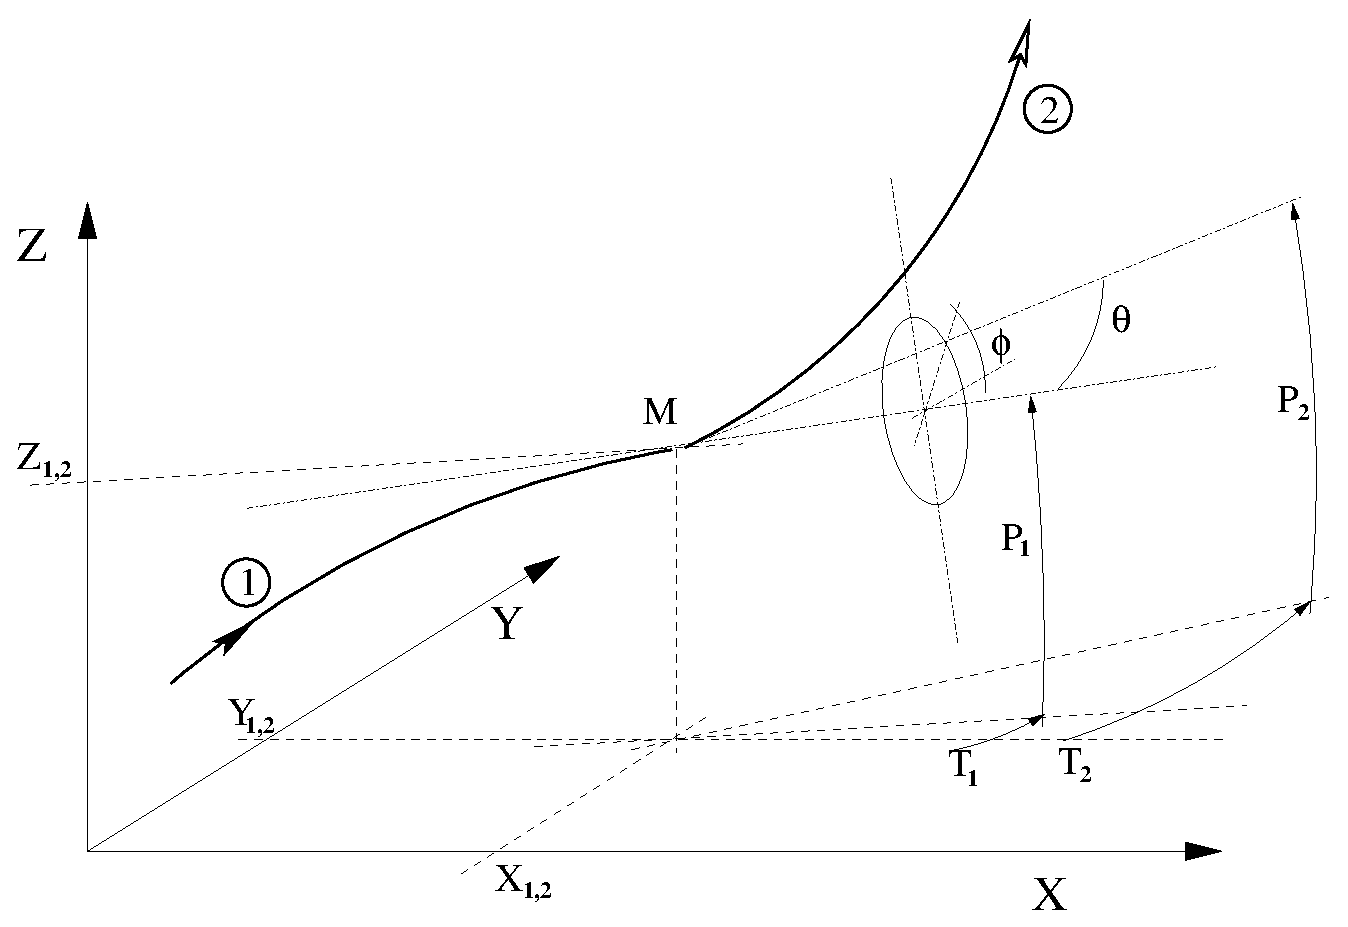
\includegraphics[width=12cm]{Fig6.eps}}
}
{\setlength{\captionwidth}{15cm}
\hangcaption[Fig6]{\label{fig6}%
At position $ M(X_1,Y_1,Z_1) $, particle~1 decays into 2 and 3~; \zgou\ then 
proceeds with the computation of the trajectory of~2, while 
3 is discarded. \\ 
$\theta$ and $\phi$ are the scattering angles of particle 2 relative to the 
direction of  the incoming particle 1~; they transform to $ T_2 $ and $ P_2 $ 
in \zgou\ frame.}       }
\end{figure}

\noindent In   \textsl{ESL\index{ESL}}   and  \textsl{CHANGREF\index{CHANGREF}},  
$ F(6,I) $ is compared to $ s $ at the
end of the element. If the decay occurs inside the element, the particle is considered as having 
decayed at its actual limit path length $ s$,  thus its coordinates 
at $ s $ are recalculated by translation.  
\bigskip

\noindent The limit path length of all particles  ($I=1$, \IMAX\index{IMAX@{\IMAX}})   is stored in
the array  \textsl{FDES}$(6,I)$.  
For further statistical purposes
(\emph{e.g.}, use of \textsl{HISTO\index{HISTO}}) the daughter  particle~2   \index{tag, tag character} 
is tagged with an $ 'S' $ standing for ``secondary''. When a particle decays, 
its coordinates $ D$, $Y$, $T$, $Z$, $P $, $s$, \textsl{time} at the decay point are stored in  
\textsl{FDES}$(J,I)$, \mbox{$ J=1,\, 7$}.  
\bigskip

\noindent \textsl {A  note}  on negative drifts~: \\
The use  of  negative  drifts  with  \textsl{MCDESINT\index{MCDESINT}}  is  allowed 
and correct. 
For instance,  negative drifts  may  occur  in  a  structure   for 
some  of  the  particles  when  using  \CHANGREF\index{CHANGREF} (due to  the  $ Z$-axis 
rotation  or  a negative  \textsl{XCE)},  or  when  using  \textsl{DRIFT}  with 
$\XL<0$. 
Provision  has  been  made  to  take  it  into  account during  the \textsl{MCDESINT\index{MCDESINT}}
 procedure,  as follows. 

\noindent If, due   to  a  negative  drift,   a  secondary  particle  reaches 
back the  decay location of its parent particle, then 
the parent  particle  is  ``resurrected `` with its original coordinates 
at  that  location, the   secondary   particle   is   discarded, and 
ray-tracing  resumes  in  a  regular way  for the parent  particle which  
is again allowed to decay,  after  the  same path length. This  procedure  is made 
possible  by  prior storage  of  the  coordinates of the parent  
particles (in array \textsl{FDES}$(J,I)$) each  time  a  decay  occurs. 

\noindent Negative steps\index{integration step size!negative}\index{XPAS!negative} (\textsl{XPAS}$<0$) in
optical elements are not compatible with  \textsl{MCDESINT\index{MCDESINT}}.  







\newpage

\subsubsection*{OPTICS~: \OPTICSTitl} \label{OPTICS} \index{OPTICS|textbf}

\medskip

\textsl{OPTICS}  normally appears next to object definition, it normally works in conjunction with 
element label(s). 

\noindent \textsl{OPTICS}  causes the transport and  write out, in zgoubi.res, of the 6$\times$6 beam matrix, 
following options \textsl{KOPT} and '\textsl{label}', below. 

~

\noindent IF \textsl{KOPT=0}~: Off

\noindent IF \textsl{KOPT=1}~: Will transport the optical functions with initial values as specified in \textsl{OBJET}, option 
 \textsl{KOBJ=5.01}. 

\medskip

\noindent  Note~:  The initial values  in \textsl{OBJET[KOBJ=5.01]} may be the periodic ones, as obtained, for instance, from a first run using \textsl{MATRIX[IFOC=11]}. 

\bigskip

\noindent A second argument,  '\textsl{label}',  allows 

- if \textsl{label~=~all}~: printing out, into zgoubi.res, after all keywords of the zgoubi.dat structure, 

- otherwise, printing out at all keyword featuring 
\textsl{LABEL}~$\equiv$~\textsl{label} as a first label  (see section~\ref{sec4.6.8}, page~\pageref{sec4.6.8}, regarding  
the labelling of keywords).


\bigskip

\noindent A third argument, \textsl{IMP=1}, will cause saving of the transported beta functions into 
file \index{zgoubi.OPTICS.out|textbf}zgoubi.OPTICS.out.








\newpage

\subsubsection*{OPTIONS~: \OPTIONSTitl} \label{OPTIONS} \index{OPTIONS|textbf}

\medskip

\textsl{OPTIONS} allows switching various options. 

~

\noindent Available, for now~: 

~

\noindent - Inhibit (most of) write statements to zgoubi.res

Form of the statement~: ``WRITE ~ ~   -1''

Back to normal~: ``WRITE ~ ~  +1''










 \newpage

\subsubsection*{ORDRE~: \ORDRETitl } \label{ORDRE} \index{ORDRE|textbf}
\medskip

 The position $ \vec  R $ and velocity $ \vec  u $ of a particle are
obtained from Taylor expansions as described in eq.~(\ref{eq2-2-4}). By default, these 
expansions are up to the fifth order derivative of $ \vec  u$, 

\begin{align*}
	\vec  R_1 
	     & \approx  \vec  R_0 + \vec  u \Delta s +...+ \vec u^{(5)} \, \dfrac{\Delta s^6 }{ 6!} \\
	\vec  u_1 
	     & \approx  \vec  u + \vec  u^{\,\prime} \Delta s  
	        + \ldots + \vec  u^{(5)}\, \dfrac{\Delta s^5 }{ 5!}   
\end{align*}
%
 which corresponds to fourth order derivatives of fields $ \vec  B $, eq.~(\ref{eq2-2-6}).
 and of $ \vec  E $, eq.~(\ref{eq2-2-10}). 

\smallskip

\noindent However, third or  higher order derivatives of fields  may be zero in some 
optical elements, for instance in a sharp edge quadrupole. Also, in 
several elements, no more than  first and second order field 
derivatives  are implemented in the code.  One may also wish to save on computation time by 
limiting the time-consuming calculation of lengthy (while possibly ineffective in terms 
of accuracy) Taylor expansions. 

\bigskip

\noindent In that spirit, the purpose of \textsl{ORDRE}, option $ IO=2-5$,  is to allow for 
expansions  to the  $ \vec  u^{(n)}$ term  in eq.~\ref{eq2-2-4}. Default functioning 
is $IO=4$, stated in \FORTRAN\ file \texttt{block.f}.

\bigskip

\noindent Note the following~: 

\noindent As concerns the optical elements
\begin{center}
	\textsl{
   DECAPOLE, DODECAPO,  EBMULT, ELMULT, 
	MULTIPOL, OCTUPOLE,   \\
              QUADRUPO, SEXTUPOL}\index{QUADRUPO}\index{SEXTUPOL}\index{OCTUPOLE}
	\index{DECAPOLE}\index{DODECAPO}\index{MULTIPOL}\index{ELMULT}\index{EBMULT} 
\end{center}
field derivatives (see eq.~\ref{eq2-2-7} p.~\pageref{eq2-2-7}, eq.~\ref{eq2-2-12} p.~\pageref{eq2-2-12},) 
have been installed in the code according 
to $ \vec  u^{(5)}$ Taylor development order~; it may not 
be as complete for  other optical elements. In particular, 
in electric optical elements field  derivatives (eq.~\ref{eq2-2-12}) are usually provided to no more than second 
order, which justifies saving on computing time by means of \textsl{ORDRE}, 
so to avoid pushing Taylor expansions as high as  $ \vec  u^{(5)}$. 


\bigskip

\noindent\textbf{NOTE}~: see also the option \textsl{IORDRE\index{IORDRE}} in field map
declarations (\textsl{DIPOLE-M, TOSCA\index{TOSCA}}, etc.).  



 \newpage

\subsubsection*{PARTICUL~: \PARTICULTitl}  \label{PARTICUL} \index{PARTICUL|textbf}
\medskip 

Since \zgoubi\ works  using the rigidity, (\BORO, as declared in \textsl{[MC]OBJET}), 
\textsl{PARTICUL} only needs  be introduced (normally, following \textsl{[MC]OBJET} in the input data file zgoubi.dat) 
 when  the definition of some characteristics of the particles 
(mass, charge, gyromagnetic factor, life-time in the 
center of mass)  is needed, as is the case when using the following procedures~: 

\bigskip           

\begin{tabular}{>{\sl}l!{~:}l}
  CAVITE    & mass,  charge \\
  MCDESINT  & mass,  COM  life-time\\
  SPNTRK    & mass,  gyromagnetic factor \\
  SRLOSS    & mass, charge \\
  SYNRAD    & mass, charge \\
  Electric and Electro-Magnetic elements
            & mass, charge 
\end{tabular}
\bigskip           

\noindent The declaration of \textsl{PARTICUL} must \textbf{precede} these keywords. 

\medskip

\noindent
If \textsl{PARTICUL} is omitted, which is in general the case when ray-tracing ions
in purely magnetic optical assemblies, then \zgoubi, since it  only knows the rigidity, 
 will  skip the computation of  such quantities as  time of flight. 



 \newpage

\subsubsection*{REBELOTE~: \REBELOTETitl} \label{REBELOTE}   \index{REBELOTE|textbf} \index{REBELOTE}\index{multi-particle}\index{multi-turn tracking|textbf}\index{acceleration} \index{synchrotron motion}
\medskip


When \REBELOTE\ is encountered in the input data file, the code execution jumps, 

- either back to the beginning of the data file - the default behavior,  

- or (option \textsl{K=99.1} or \textsl{K=99.2}) back to a particular \LABEL. 

\noindent  Then  \textsl{NPASS-1}\index{NPASS} passes (from \LABEL\ to  \REBELOTE) follow.  

\noindent As to the last pass, number  \textsl{NPASS+1}, there are two possibilities~: 

- either it also encompasses the whole \LABEL\ to  \REBELOTE\ range, 

- or, upon request (option \textsl{K=99.2}),  execution may exit that final  pass upstream of 
\textsl{REBELOTE}, at a location defined by a second   dedicated \LABEL\ placed  between 
the first above mentioned \LABEL, and \REBELOTE. 
In both cases, following the end of this ``multiple-pass'' procedure, 
the execution  continues from the keyword which follows \REBELOTE, until \textsl{'END'} is encountered. 

\bigskip

The two functionalities of \textsl{REBELOTE} are the following~: 

\smallskip

\noindent {\small $\bullet$} \REBELOTE\ can be used for Monte Carlo\index{Monte Carlo} simulations when more 
than Max(\IMAX) particles  \index{IMAX@{\IMAX}} are to be tracked. 
Thus, when the following random procedures 
are used~: \textsl{MCOBJET\index{MCOBJET}, OBJETA\index{OBJETA}, MCDESINT\index{MCDESINT}, 
SPNTRK\index{SPNTRK}} \mbox{(\textsl{KSO} = 5)},
their random seeds are not reset and  independent statistics will add up. 

\noindent This includes  \textbf{Monte Carlo simulations}, in beam lines~: normally $ K=0$.  \textsl{NPASS}\index{NPASS} runs
through the same structure, from \textsl{MCOBJET} to \textsl{REBELOTE} will follow, resulting in the calculation of 
$(1+\text{\textsl{NPASS}})  \ast  \text{\IMAX}$ trajectories, with as many random initial coordinates. 

\bigskip

\noindent {\small $\bullet$} \REBELOTE\ can be used for  multi-turn ray-tracing  \index{multi-turn tracking} 
in circular machines \textbf{circular machines}~: normally $ K=99$ in that case.  \textsl{NPASS} turns in
the same structure will follow, resulting in the tracking of \IMAX\ 
particles over $1+\text{\textsl{NPASS}}$ turns. For the simulation of 
pulsed power supplies, synchrotron motion, and other Q-jump manipulation, see \textsl{SCALING}. 

\noindent For instance, using option described \textsl{K=99.2} above, a full ``injection line + ring + extraction line'' installation 
can be simulated - kicker firing  and other magnet ramping can be simulated using \textsl{SCALING}. 

\noindent Using the double-\LABEL\ method discussed above with option \textsl{K=99.2}, it is possible to encompass the ring between 
an injection line section (namely, with the element sequence of the latter extending from \OBJET\ to the first \LABEL), 
and an extraction line (its description will then follow \REBELOTE), 
whereas the ring description extends  from  to the first \LABEL\ to \REBELOTE, 
with possible extraction, at the last pass, at the location of the second \LABEL, located between the first one and \REBELOTE, 

\bigskip

In addition to what precedes,  \textsl{REBELOTE} can change the value of arbitrary parameters in zgoubi.dat 
data list. \textsl{NPRM} tells the number of parameters to be changed. 
A series of   \textsl{NPRM} lists of values, one list per parameter to be changed and each list 
with \textsl{NRBLT} data, tells the 
 values to be taken by each one of these parameters, over the \textsl{NRBLT} passes of the 
\textsl{REBELOTE} process.  

\bigskip

\noindent Output prints over \textsl{NPASS+1} passes  might result in a
prohibitively big zgoubi.res file. They may be switched on/off  by means of the option 
\mbox{\textsl{KWRIT}$= i.j$}, with $i=1/0$ respectively. The $j$ flag commands printing 
pass number and some other information onto the video output, every $10^{j-1}$ turns if $j>0$~; output is switched  
off if $j=0$. 

  
\bigskip

\noindent\REBELOTE\ also provides information~: statistical calculations and related 
data regarding particle decay \textsl{(MCDESINT\index{MCDESINT})}, spin tracking\index{spin tracking}  
\textsl{(SPNTRK\index{SPNTRK})}, stopped particles\index{stopped particles} (\textsl{CHAMBR\index{CHAMBR},
 COLLIMA\index{COLLIMA}}), etc.  




\bigskip

\paragraph{\textit{COMBINING REBELOTE AND FIT[2]} \index{REBELOTE and FIT, combined|textbf}}    %%%%[10]


\noindent The keyword  \textsl{REBELOTE}  can follow   \textsl{FIT[2]}.  This allows executing again 
the same fit procedure,  after having changed the value of some parameter in zgoubi.dat. 
That's the role of   \textsl{REBELOTE}  in that game~: it changes that parameter, and then sends the 
zgoubi execution pointer back to the top of zgoubi.dat for a new run. 


\bigskip

 An example of the use of the \textsl{REBELOTE} procedure is given page~\pageref{ExaREBELOTE}. 

\bigskip

 An example combining \textsl{FIT} and \textsl{REBELOTE} is given page~\pageref{ExaFITREBELOTE}. 




\newpage

\subsubsection*{RESET~: \textbf{\RESETTitl} } \label{RESET} \index{RESET|textbf}
\medskip 

 \noindent Resets counters involved  in \textsl{CHAMBR}\index{CHAMBR}, \textsl{COLLIMA}\index{COLLIMA},   
  \textsl{HISTO}\index{HISTO} and \textsl{INTEG}\index{INTEG} procedures. 
 
~

 \noindent Switches off \textsl{CHAMBR}, \textsl{MCDESINT}\index{MCDESINT}, \textsl{SCALING}\index{SCALING} and 
 \textsl{SPNTRK}\index{SPNTRK} options. 






 \newpage

\subsubsection*{SCALING~: \SCALINGTitl} \label{SCALING} \index{SCALING|textbf} \index{multi-turn tracking}
\medskip 
\index{synchrotron motion}

\textsl{SCALING} acts as a function generator dedicated to varying 
fields in optical elements, potentials in 
electrostatic devices, RF parameters in \textsl{CAVITE\index{CAVITE}}. It is normally intended
to be declared right after the object definition, and used in conjunction 
with \textsl{REBELOTE\index{REBELOTE}}, for the simulation of multi-turn tracking 
- possibly including  acceleration  \index{acceleration} cycles.  

\bigskip

\noindent\textsl{SCALING} acts on families of elements,  a family being
designated by its name that  coincides with 
the keyword of the corresponding element. For instance, declaring \textsl{MULTIPOL\index{MULTIPOL}} 
as to be varied will result in the same timing law being applied to all 
\textsl{MULTIPOL\index{MULTIPOL}}'s in the \zgou\ optical structure data file. Subsets can be selected by 
labeling keywords in the data file (section~\ref{sec4.6.8}, page~\pageref{sec4.6.8}) 
and adding the corresponding \LABEL(s)\index{LABEL@{\LABEL}} 
in the \textsl{SCALING} declarations (two \LABEL's maximum). The family name of concern, 
as well as the scaling function for  that  family,  are given as
input data to the keyword \textsl{SCALING\index{SCALING}}. There is an upper limit, \textsl{NFMAX}, to the number  $NF$ 
of families that can be declared
as subject to a scaling law,  \textsl{NFMAX} can be changed in the \FORTRAN\ include file \texttt{MXFS.H}. 
A scaling law can be comprised  of up to $NT$~successive timings,  
between two successive timings, a linear interpolation law is used to determine the scaling factor. 

\bigskip

\noindent An example of data formatting for the simulation of an acceleration cycle in a circular 
machine is given in the following. 

\bigskip

{\small
{\renewcommand{\arraystretch}{1}
\noindent\begin{tabular}{lll}
  \textsl{SCALING}    &          & - Scaling \\
  1    ~~~~ 4         &          &  Active. $NF = 4$ families of elements are concerned, as listed below \\
  \textsl{QUADRUPO} \textsl{QFA} \textsl{QFB}&          & - Quadrupoles labeled 'QFA' and Quadrupoles labeled 'QFB' \\
  2                   &          & $NT = 2$ timings  \\
  18131.E-3           & 24176.E-3 \qquad 
                                 &   The field increases (linearly) from 18131E-3$\ast B_0 $ 
                                 to 24176E-3$\ast B_0 $  \\
  1                   & 6379     &  from turn 1 to turn 6379\\
  \textsl{MULTIPOL} \textsl{QDA} \textsl{QDB}&          &- Multipoles labeled 'QDA' and Multipoles labeled 'QDB'\\
  2                      &       &      $NT = 2$ timings  \\
  18131.E-3           &24176.E-3 &  Fields  increase from 18131E-3$\ast {B_i} $ to 
                                  24176E-3$\ast  {B_i} $  ($\forall i=1,\,10$ poles) \\
  1                   & 6379     & from turn 1 to turn 6379\\
  \textsl{BEND}       &          &- All \textsl{BEND}'s (regardless of any \LABEL) \\
  2                  &               &           $NT = 2$ timings  \\
  18131.E-3           &24176.E-3 & As above \\
  1                   & 6379  \\
  \textsl{CAVITE}     &          &- Accelerating cavity \\
  3                      &           &         $NT = 3$ timings  \\
  1 ~~~~~ 1.22        &1.33352   &The synchronous rigidity $(\Br )_s $ increases, \\
  1 ~~~~~   1200      & 6379     &from $ (\Br )_{s_o} $ to 1.22 $\ast (\Br)_{s_o} $ from turn 1 to 1200, and \\
                      &          &from 1.22 $\ast (\Br)_{s_o} $ to 1.33352 $ (\Br )_{s_o} $ from turn 1200 to 6379 
\end{tabular} }                   
}

 \bigskip

\noindent The timing is in unit of turns. In this example, TIMING = 1 to 6379 
(turns). Therefore, at turn number $ N, ~ B $ and $ B_i $ are updated in the 
following way. Let \textsl{SCALE}(\textsl{TIMING} $ = N$) be the updating scale factor

\begin{align*}
   \text{SCALE}(N) & = 18.131 \dfrac{24.176-18.131 }{ 1+6379-1} (N-1)  \\
\intertext{and then}
     B(N)   &  = \text{\textsl{SCALE}}(N)B_0 \\ 
     B_i(N) &  = \text{\textsl{SCALE}}(N){B_i}_0 \\
\intertext{The  RF frequency is computed using}
     f_{RF} & = \dfrac{hc }{\mathcal{L}} \, 
              \dfrac{q(\Br )_s }{ (q^2(\Br )^2_s + (Mc^2)^2)^{1/2}} 
\end{align*}
%
where the rigidity is updated in the following way. Let $ (\Br)_{s_o} $ be the 
initial rigidity (namely, $ (\Br )_{s_o}= $ \BORO\ as defined in the keyword
\textsl{OBJET} for instance). Then, at turn number $ N$,   

\begin{alignat*}{2}
	\text{if  }   1 & \leq N\leq 1200 \,          
	            & \text{  then,  \textsl{SCALE}}(N)  & =1+ \dfrac{1.22-1 }{ 1+1200-1}\, (N-1) \\
	\text{if  }   1200 & \leq N\leq 6379 \,           
	            & \text{  then,  \textsl{SCALE}}(N)  & =1.22+ \dfrac{1.33352-1.22 }{ 1+6379-1200}\,(N-1200)    
\end{alignat*}
 
 \noindent and then, 

$$ (\Br )_s(N) = \text{\textsl{SCALE}}(N)\cdot (\Br )_{s_o} $$
%
from which value the calculations of $ f_{RF}(N) $ follow. 


\bigskip

 \noindent $NT$ can take negative values, then acting as an option switch (rather than giving number of timings), as follows~: 

 \noindent $\bullet ~ NT = -1$~: this is convenient for synchrotron acceleration. In this case 
the next two lines both contain a single data (as for $NT=1$), respectively the starting scaling factor value, and 1.  
The current field scaling factor will  then be  updated 
 from the energy kick by the cavity if for instance \textsl{CAVITE/IOPT=2} is used, namely, 
\begin{align*}
   \text{SCALE}(N) & = \text{SCALE}(N-1) * \dfrac{B\rho(N)}{B\rho(N-1)}  \\
\end{align*}


 \noindent $\bullet ~ NT = -2$~: this is convenient for reading an RF law for \textsl{CAVITE} from an external data file, 
including usage for acceleration in fixed field accelerators. 


 \noindent $\bullet ~ NT = 1.10$~: allows taking the scaling law from an external data file, as in the following example~:

\bigskip

{\renewcommand{\arraystretch}{1}
\noindent	\begin{tabular}{lll}
MULTIPOL COH1  \\
1.10             \\
./Csnk3D/bump\_centered.scal & ~ ~ ~ ~ ~ ~ ~ ~& File name \\
1   2  &     &  Column numbers in the file~: col.~2 gives the scaling \\[-.8ex]
       &      &  factor at rigidity given by col.~1. \\
	\end{tabular}   }

\bigskip

\noindent {\bf Notes~:} 

\medskip

\noindent 1. In causing, via \textsl{CAVITE}, a change of the synchronous rigidity, \textsl{SCALING} causes 
a change of the reference rigidity, following (see \textsl{CAVITE})    \index{reference rigidity} 

$$B\rho_{ref} = \BORO \longrightarrow B\rho_{ref} = \BORO + \delta \Br_s$$ \index{BORO@{\BORO}$\times D_{ref}$}


\medskip

\noindent 2. It may happen that some optical elements won't scale, for source code development reasons. 
This should be paid attention to. 



\newpage

\subsubsection*{SPNTRK~: \SPNTRKTitl} \label{SPNTRK} \index{SPNTRK|textbf}
\medskip

The keyword \textsl{SPNTRK} allows switching  spin tracking\index{spin tracking} on (index \textsl{KSO}=1) or off (\textsl{KSO}=0), 
or resuming (index \textsl{KSO}=-1, following an occurence \textsl{KSO}=0). 
 It also permits the attribution of an initial spin to each one of the 
\IMAX\index{IMAX@{\IMAX}} particles of the beam, following a distribution that depends 
on the option index \textsl{KSO}. It must be preceded by \textsl{PARTICUL\index{PARTICUL}} for
the definition of  mass and gyromagnetic factor.  
\medskip

\noindent\textbf{KSO = 1  (respectively 2, 3)~:} the \IMAX\ particles
 defined with \textsl{[MC]OBJET} are given a longitudinal (1,0,0) spin component (respectively 
transverse horizontal (0,1,0), vertical (0,0,1)).  
\medskip

\noindent\textbf{KSO = 4~:} initial spin components are entered explicitly for
each one of the \IMAX\index{IMAX@{\IMAX}} particles of the beam.  
\medskip

\noindent\textbf{KSO = 4.1~:} three initial spin components $S_X, ~S_Y, ~S_Z$ are entered explicitly just once, 
they are then assigned to  each one of the \IMAX\index{IMAX@{\IMAX}} particles of the beam.  
\medskip

\noindent\textbf{KSO = 5~:} random generation of \IMAX\index{IMAX@{\IMAX}} initial spin
conditions as described in Fig.~\ref{fig7}.  
Given a mean polarization axis (S) defined by its angles $ T_0 $ and $ P_0 $, 
and a cone of angle~A with respect to this axis, the \IMAX\index{IMAX@{\IMAX}} spins are sorted randomly in a 
Gaussian distribution

$$ p(a) = \exp \left[- \dfrac{(A-a)^2 }{ 2\delta A^2} \right]/ \delta A\,  \sqrt{2\pi}   $$
%
and within a cylindrical uniform distribution around the (S) 
axis. Examples of simple distributions available by this mean are 
given in Fig.~\ref{fig8}.  


%%%%%%%%%%%%%%figure%%%%%%%%%%%%%%
\begin{figure}[H]
%\vspace{11 truecm}
%%%Figure 7
\centerline{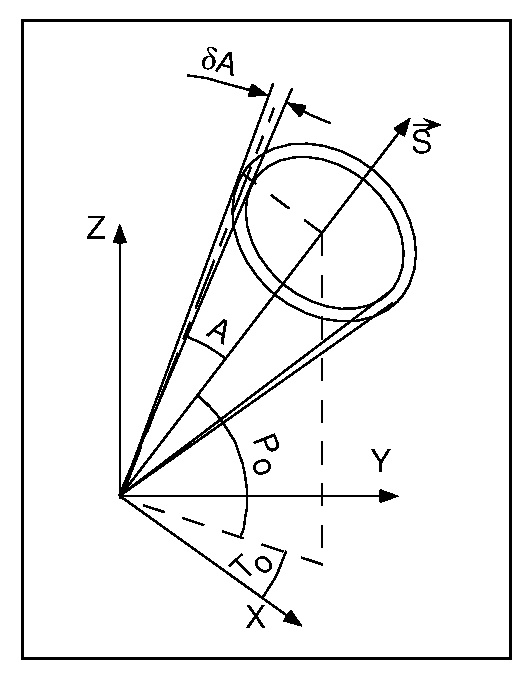
\includegraphics[height=10cm]{Fig7.ps}}
{\setlength{\captionwidth}{12cm}
\hangcaption[Fig7]{\label{fig7}Spin distribution as obtained with option \textsl{KSO} = 5.\\
          The spins are distributed within an annular strip 
         $\delta A$ (standard deviation)  
          at an angle $A$ with respect to the 
         axis of mean polarization (S) defined by $T_0$  and $P_0$.} 
}\end{figure}
%%%%%%%%%%%%%%figure%%%%%%%%%%%%%%
%\figureh 5cm   \figurev 7cm  
\begin{figure}[H]
%\vspace{8.5 truecm}
%%%Figure 8
\centerline{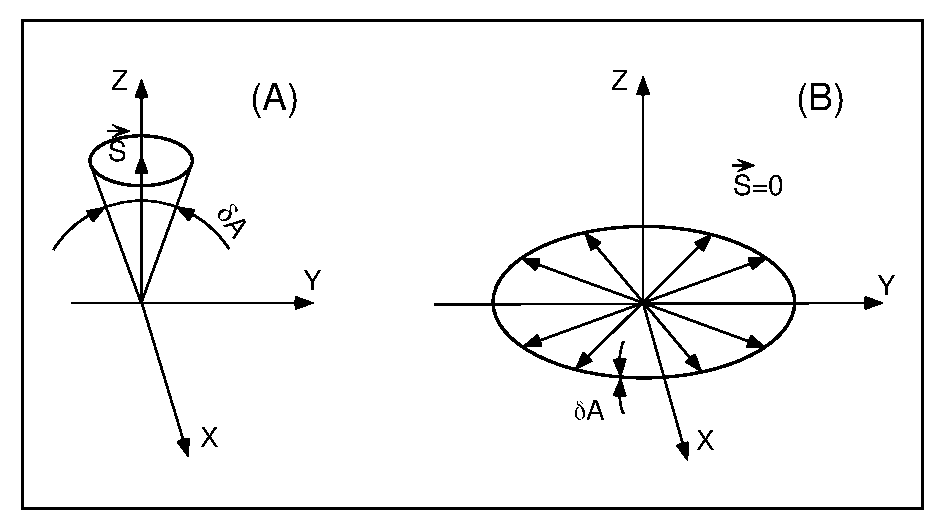
\includegraphics[width=15cm]{Fig8.ps}}
{\setlength{\captionwidth}{14cm}
\hangcaption[Fig8]{\label{fig8}Examples of the use of	\textsl{KSO} =5. \\
A~: Gaussian	distribution around	a mean vertical	polarization axis, 
 obtained   with	$T_0$  = arbitrary,	$P_0 = \pi /2$,	$A = 0$ and $\delta A \not=  0$.\\
B~: Isotropic distribution in the median	plane, obtained	with 
 $P_0 =	\pm	 \pi /2$, 
$A = \pi /2$,	and	$\delta	A =	0$.} }
 \end{figure}
\newpage

\subsubsection*{SRLOSS~: \SRLOSSTitl\ \cite{FMSEA-00-01} } \index{SRLOSS|textbf}\label{SRLOSS}
\medskip 
\index{synchrotron radiation loss}

\noindent The keyword \textsl{SRLOSS} allows activating or stopping (option $\KSR=1,0$ respectively) 
 stepwise tracking  of energy loss by stochastic emission of 
photons in magnetic fields, following the method described in section~\ref{SRLoss}.  

\bigskip

\noindent  It can be chosen to allow radiation in the sole dipole fields, or in all types of fields regardless of 
their multipole composition.  It can also be chosen to allow for the radiation induced transverse kick. 

\bigskip

\noindent  \textsl{SRLOSS}  must be preceded by \textsl{PARTICUL}\index{PARTICUL} for defining  mass and charge 
values as they enter in the definition of SR parameters. 


\bigskip

\noindent  Statistics on SR parameters are  computed and updated while tracking, the results of which can be obtained by means of 
the keyword  \textsl{SRPRNT}\index{SPNPRT}. 


\newpage

\subsubsection*{SYNRAD~: \SYNRADTitl}\label{SYNRAD}\index{SYNRAD|textbf}\index{synchrotron radiation spectra}
\medskip 

\noindent The keyword \textsl{SYNRAD} enables (or disables) the calculation of 
synchrotron radiation (SR) electric field and spectral angular energy density. It must be 
preceded by \textsl{PARTICUL}\index{PARTICUL} for defining  mass and charge values, as they enter 
in the definition of SR parameters. 

\bigskip

\noindent\textsl{SYNRAD} is supposed to appear a first time at the 
location where SR should start being taken into account, with the first data \textsl{\KSR} set 
to~1. It results in on-line storage of the electric field vector and 
other relevant quantities in zgoubi.sre\index{zgoubi.sre}, as step by step integration 
proceeds. The observer position ($XO$, $YO$, $ZO$) is specified next 
to \textsl{\KSR}.

\bigskip

\noindent Data stored in zgoubi.sre~:
 
 \begin{tabular}{l} 
 ($ELx$, $ELy$, $ELz$)~:  electric field vector $\vec\Ecal $ 
 						(eq.~\ref{eqN4.1}) \\
 $(btx, bty, btz) = \vec\beta= \dfrac{1}{c} \times$ particle velocity \\
$(gx, gy, gz) = \dfrac{d\vec\beta}{dt} =$ particle acceleration (eq.~\ref{eqN4.3}) \\					
$\Delta \tau =$ observer time increment (eq.~\ref{eqN4.2}) \\
$t' = \tau  - r(t')/c = $ retarded (particle) time \\
$(rtx, rty, rtz)~: \vec R(t)$, particle to observer vector (eq.~\ref{eqN4.4}) \\
$(x, y, z) =$ particle coordinates\\
$\Delta s = $ step size in the magnet (fig.~\ref{fig2})\\
$NS=$ step number\\
$I=$ particle number\\
$LET(I)=$ tagging letter\\      \index{tag, tag character} 
$\IEX(I)\index{IEX@{\IEX}}=$ stop flag (see section~\ref{sec4.6.6}) 
\end{tabular}
\bigskip


\noindent\textsl{SYNRAD} is supposed to appear a second time at the 
location where SR~calculations should stop, with \textsl{\KSR} set 
to~2. It results in the output of the angular energy density 
$\int_{\nu_1}^{\nu_2} \partial^3 W / \partial \phi \, \partial \psi 
\, \partial \nu$ (eq.~\ref{eqN4.11}) as calculated from the Fourier transform 
of the electric field (eq.~\ref{eqN4.11}). The spectral range of 
interest and frequency sampling ($\nu_1$, $\nu_2$, $N$) are specified 
next to \textsl{\KSR}.
\bigskip



\newpage

\subsubsection*{SYSTEM~: \SYSTEMTitl}\label{SYSTEM}\index{SYSTEM|textbf}\index{system call}
\medskip 

\noindent The keyword \textsl{SYSTEM} allows one or a series of system calls. 
It can appear anywhere, an arbitrary number of times, 
 in the zgoubi.dat data list. It is effective at the very location where it appears. 

\medskip 

\noindent  \textsl{SYSTEM} keyword is followed by the list of the desired system commands. That 
can be saving zgoubi output files, calling again \zgou\ at the end of a run so allowing 
dependent consecutive jobs, etc. 




\clearemptydoublepage


\subsection{Optical Elements and Related Numerical Procedures} \label{sec4.4}


\subsection*{AGSMM~:  \AGSMMTitl} \label{AGSMM}\index{AGSMM|textbf}
\medskip 


The AGS main magnet is a combined function dipole with straight axis (lines of constant field are straight lines).  

\noindent The field computation routines for   \textsl{AGSMM}  are the same as for \textsl{MULTIPOL} 
(details in section~\ref{sec2.3.5}, page~\pageref{sec2.3.5}), 
however  \textsl{AGSMM}  has  the following four particularities~: 

\begin{itemize}
  \item There are only three multipole components present in \textsl{AGSMM}~: dipole, quadrupole and sextupole. 
  \item The dipole field $B_0$ is drawn from the reference rigidity, $B\rho_{ref}$, and  follows the latter so to preserve 
$\rho = B\rho_{ref} / B_0$  and the orbit deviation  $L/\rho$. In particular, 
  \begin{itemize}
     \item in the absence of acceleration, $B\rho_{ref} \equiv BORO$, with $BORO$ the quantity appearing  in the object definition 
using  \textsl{[MC]OBJET}, 
     \item in presence of acceleration using \textsl{CAVITE}, $B\rho_{ref} $ is changed 
to $ BORO\times D_{ref}$  \index{BORO@{\BORO}$\times D_{ref}$} at each passage in the cavity, with $D_{ref}$ 
the relative synchronous momentum increase, a quantity that \zgou\ updates at cavity traversal.
  \end{itemize}
  \item The field indices, quadrupole $K1$ and sextupole $K2$, are derived from  the reference rigidity, $B\rho_{ref}$, via 
 momentum-dependent polynomials, taken from Ref.~\cite{EJBleser}.  

  \item The AGS main dipole has back-leg windings, used for instance for injection and extraction orbit bumps. 
The number of winding turns and the  number of Ampere-turns 
are part of the data in the input data list. The intensity in the windings is  accounted for in the conversion 
 from total ampere-turns in the magnet  to momentum and then to magnetic field. 
\end{itemize}

\bigskip

  \noindent Note~: A consequence of  items~2 and~3 is that  no field value is required in defining the AGS main magnets in 
the  zgoubi.dat input data list. 




\newpage

\subsubsection*{AGSQUAD~:  \AGSQUADTitl} \label{AGSQUAD}\index{AGSQUAD|textbf}
\medskip 

The AGS quadrupoles are regular quadrupoles. 
The simulation of  \textsl{AGSQUAD}  uses the same field modelling as \textsl{MULTIPOL}, 
section~\ref{sec2.3.5}, page~\pageref{sec2.3.5}.  However amperes are provided as input to 
 \textsl{AGSQUAD} rather than fields, the reason being that 
 some of the AGS quadrupoles  have two superimposed coil circuits, with separate power supplies. 
It has been dealt with this 
particularity by allowing  for an additional set of quadrupole data in \textsl{AGSQUAD}, compared to \textsl{MULTIPOL}. 

\bigskip

\noindent The field in \textsl{AGSQUAD} is computed using transfer functions from the ampere-turns in the coils to 
magnetic field that  account for the non-linearity of the magnetic permeability~\cite{MADXAGSModel}. 



\newpage



\subsubsection*{AIMANT~:  \AIMANTTitl}\label{AIMANT}\index{AIMANT|textbf}
\medskip

The keyword \textsl{AIMANT} provides an automatic
generation of a dipole median plane field map in polar coordinates. 

\medskip
\noindent A more recent and improved version will be 
found in \textsl{DIPOLE-M\index{DIPOLE-M}}. In addition, a similar modelling, that however skips 
the stage of an intermediate mid-plane field map, can be found in  \textsl{DIPOLE[S]\index{DIPOLE}}\index{DIPOLES}.

\medskip
\noindent The extent of the map is defined by the 
following parameters, as shown in Figs.~\ref{fig9}A and~\ref{fig9}B, 

 \begin{tabular}{>{\sl}l!{~:}l}
	 AT &  total angular aperture\\
	 RM & mean radius used for the positioning of field boundaries\\
	 RMIN, RMAX
	    &  minimum and maximum radial boundaries of the map 
 \end{tabular}
\bigskip

\noindent The 2 or 3 effective field boundaries (EFB) inside the map are
defined from  geometric boundaries, the shape and position of which are determined by the 
following parameters, 


\begin{tabular}{l!{~:}l}
	 \textsl{ACENT} 
	    & arbitrary  angle, used for the positioning of the EFB's. \\
	$\omega$ &  azimuth of an EFB with respect to  \textsl{ACENT}\\
	$\theta$ & angle of a boundary with respect to its azimuth (wedge angle)\\ 
	$R_1$, $R_2$  &  radius of curvature of an EFB\\
	$U_1$, $U_2$  &  extent of the linear part of the EFB. 
\end{tabular}
\bigskip

\noindent At  any node  of the map mesh, the value of the $Z$ 
component of the field is calculated as 

 \begin{equation}
	 B_Z =  \mathcal{F}(R,\theta) \ast  B_0 \ast  
	      \left(1+N \ast  
	           \left( \dfrac{R-RM }{ RM}\right) 
	           + B \ast  \left(\dfrac{R-RM }{ RM} \right)^2 
	           + G \ast  \left(\dfrac{R-RM }{ RM} \right)^3 
	      \right) 
 	\label{eq4-4-1}
 \end{equation}
%
 where  $ N$, $B $ and $ G $ are  respectively  the first, second and
third order field indices and $ \mathcal{F}(R,\theta)$ is the fringe field 
coefficient  (it determines the ``flutter''  in periodic structures).  


\subsubsection*{Calculation of the Fringe Field Coefficient} 

With  each EFB a realistic extent of the fringe field, $\lambda$, 
is associated (Figs.~\ref{fig9}A and~\ref{fig9}B),  
and a fringe field coefficient $ F$ is 
calculated. In the following $\lambda$ stands for either $ \lambda_ E $
(Entrance), $ \lambda_ S $ (Exit) or $ \lambda_ L $ (Lateral EFB). 
 
\noindent If a node of the map mesh is at a distance of the EFB larger than
$\lambda$, then $  F=0 $ outside the field map and $ F=1 $ inside.  
If a node is inside the fringe field zone, then $  F$   is calculated as follows. 

\bigskip 

\noindent Two options are available, for the calculation of $ F$, depending
on the value of $\xi$. 

\medskip
\noindent\textbf{If } $\mathbf{\xi  \geq 0}$, $ F $ is a  second
order type fringe field (Fig.~\ref{fig11}) given by 


\begin{gather}
		F  = \dfrac{1 }{ 2} \, \dfrac{(\lambda -s)^2 }{ \lambda^2-\xi^ 2} \quad 
		         ~~ \text{if }~   \xi  \leq  s \leq \lambda  \\
		F  = 1- \dfrac{1 }{ 2} \, \dfrac{(\lambda -s)^2 }{ \lambda^2-\xi^ 2}\quad 
		        ~~ \text{if }~   -\lambda  \leq  s \leq  -\xi 
\end{gather}
where $ s $ is the distance to the EFB, and
\begin{gather}
		 F  = \dfrac{1 }{ 2} + \dfrac{s }{ \lambda +\xi} \quad
		         ~~ \text{if }~  0 \leq  s \leq  \xi  \\
	    F   = \dfrac{1 }{ 2} - \dfrac{s }{ \lambda +\xi}\quad  
		       ~~ \text{if }~   -\xi  \leq  s \leq  0  
\end{gather}
 
\noindent This simple model allows a rapid calculation of the fringe field,
but may lead to erratic behavior of the field when extrapolating out of the median plane, 
due to the discontinuity of $ d^2B/ds^2 $,  at $ s=\pm \xi $ and $ s=\pm \lambda $. 
For better  accuracy it is advised to use the next option. 

\newpage
%%%%%%%%%%%%%%figure%%%%%%%%%%%%%%
\begin{figure}[H]
%\vspace{21 truecm}
%%%Figure 9
\centering
            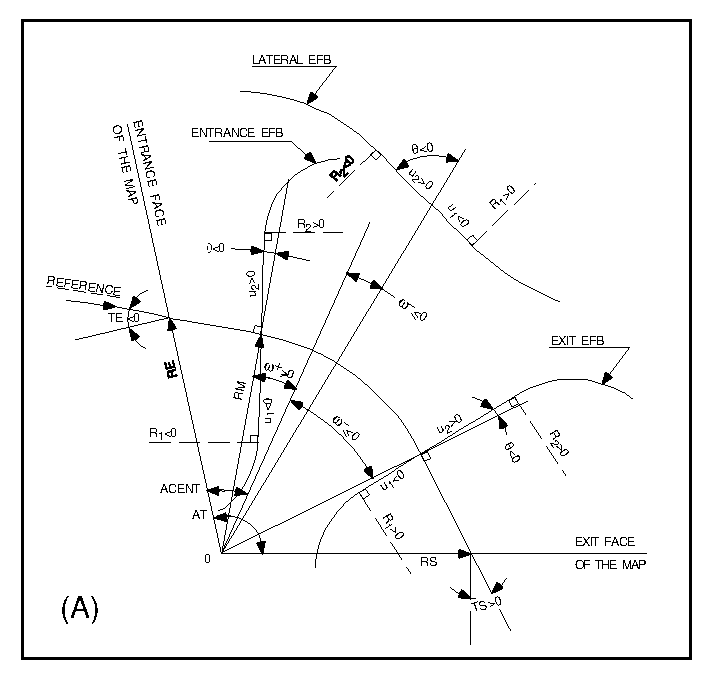
\includegraphics[width=12cm]{Fig9a.eps}
            \vfill
            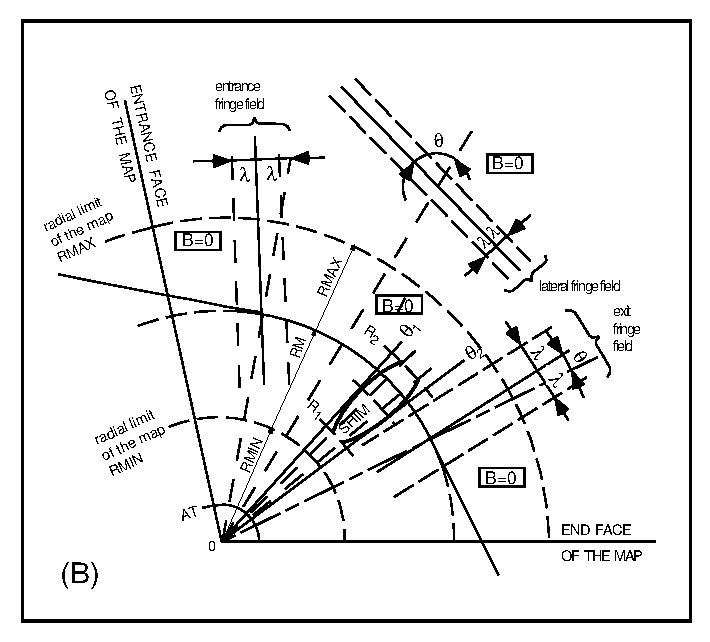
\includegraphics[width=12cm]{Fig9b.eps}
\hangcaption[Fig9]{\label{fig9} A~: Parameters used to define the field map and 
geometrical boundaries. \\
  B~: Parameters used to define the field map and fringe fields.}  
\end{figure}  
\newpage

\noindent\textbf{If $\mathbf{\xi  = -1}$},  $ F $ is an exponential type
fringe field (Fig.~\ref{fig11}) given by~\cite{Biblio12}  %%%   [12]

 \begin{gather}
	 F = \dfrac{1 }{ 1+ \exp  P(s)}
 	\label{eq4-4-4} \\
\intertext{where $ s $ is the distance to the EFB, and }
    P(s) = C_0
       +C_1 \left(  \dfrac{s }{ \lambda} \right) 
       +C_2 \left( \dfrac{s }{ \lambda} \right)^2 
       + C_3 \left( \dfrac{s }{ \lambda} \right)^3 
       +C_4 \left( \dfrac{s }{ \lambda} \right)^4 
       + C_5 \left(\dfrac{s }{ \lambda} \right)^5 \label{eq4-4-5}
\end{gather}
%
The values of the coefficients $ C_0 $ to $ C_5 $ should be such that the 
derivatives of $ B_Z$ with respect to $ s $ be negligible at $ s=\pm \lambda $, so as not
to perturb the extrapolation of $ \vec B $ out of the median plane.
%  (this restriction no longer holds in the improved version \textsl{DIPOLE-M\index{DIPOLE-M}}).  

\noindent It is also possible to simulate a shift of the EFB, by giving a non
zero value to the parameter \textsl{shift}.  $ s $ is then changed to $ s  -$~\textsl{shift} in the 
previous equation.   This allows small variations of the total 
magnetic length. 

\noindent Let $ F_E $ (respectively $ F_S$, $F_L$)   be the fringe field
coefficient attached to the entrance (respectively exit, lateral) EFB following  the equations\ above. At any
node of the map mesh, the resulting value of the fringe field coefficient (eq.~\ref{eq4-4-1}) is 
(Fig.~\ref{fig12})  

$$ \mathcal{F}(R,\theta)= F_E \ast  F_S \ast  F_L $$
%
 In particular, $F_L\equiv 1 $ if no lateral EFB is requested. 

\subsubsection*{The Mesh of the Field Map} 

The magnetic field is calculated at the nodes of a mesh with polar
coordinates, in the median plane.  The radial step is given by 
 \begin{align*}
	 \delta R & = \dfrac{\text{\textsl{RMAX - RMIN}} }{\text{\textsl{IRMAX}}-1} \\
\intertext{ and the angular step by} 
	\delta \theta  & = \dfrac{AT }{ \text{\textsl{IAMAX}}-1} 
 \end{align*}
%
\noindent where, \textsl{RMIN} and  \textsl{RMAX}   are the lower and upper
radial limits of the field map, and $ AT $ is its total angular aperture (Fig.~\ref{fig9}B).  
 \textsl{IRMAX} and  \textsl{IAMAX} are the total number of nodes in the radial and 
 angular directions. 
 

 
 \subsubsection*{Simulating Field Defects and Shims } 
 
  Once the initial map is calculated, it is possible to perturb it by
means of the parameter \textsl{NBS}, so as to simulate field defects or shims. 
\bigskip

\noindent\textbf{If} $\mathbf{NBS = -2}$, the map is globally modified by a
perturbation proportional to $ R-R_0 $, where $ R_0 $ is an arbitrary radius, 
with an amplitude $ \Delta B_Z/B_0 $, so that $ B_Z $ at the nodes of the mesh is replaced by 

$$ B_Z \ast  \left( 1+ \dfrac{\Delta B_Z }{ B_0} \,
                 \dfrac{R-R_0 }{\text{\textsl{RMAX}} - \text{\textsl{RMIN}}} \right) $$


\noindent\textbf{If} $\mathbf{NBS = -1}$, the perturbation is proportional to
$ \theta -\theta_ 0 $, and $ B_Z $ is replaced by 

$$ B_Z \ast  \left(1+ \dfrac{\Delta B_Z }{ B_0}\, \dfrac {\theta -\theta_ 0 }{ AT}\right) $$


\newpage

%%%%%%%%%%%%%%figure%%%%%%%%%%%%%%
\begin{figure}[H]
  \centering
%%%Figure 10
  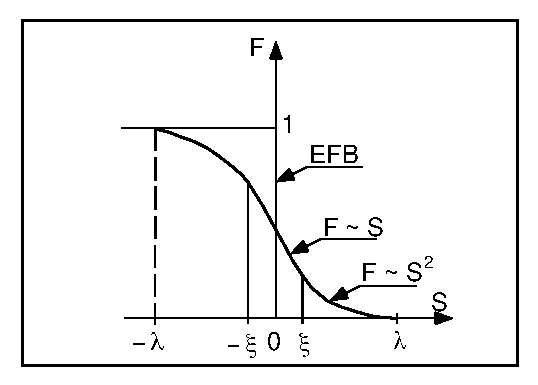
\includegraphics[width=9cm]{Fig10.ps}
  \vfill
%%%Figure 11
  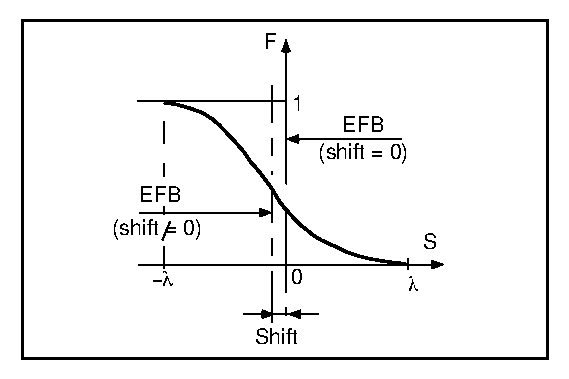
\includegraphics[width=9cm]{Fig11.ps}
{\setlength{\captionwidth}{10cm}
\hangcaption{\label{fig11}Second order type fringe field (upper plot) 
and exponential type fringe field (lower plot).}}
\end{figure}

\vfill
\begin{figure}[H]
%\vspace{10 truecm}
%%%Figure 12
\centerline{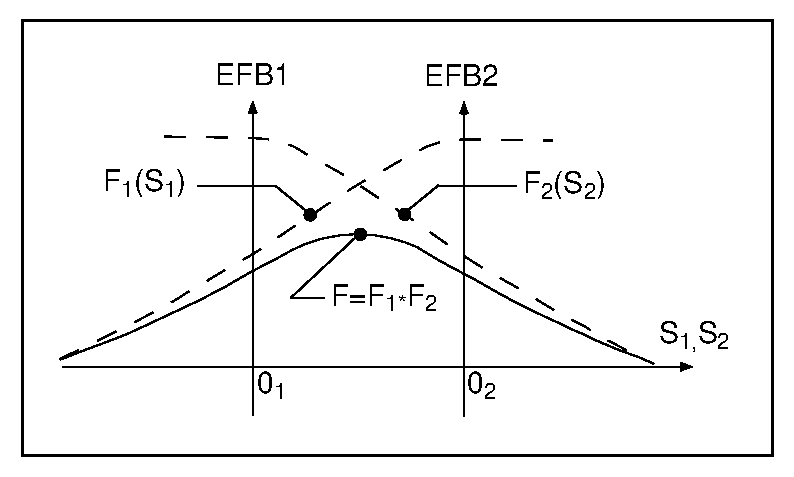
\includegraphics[width=10cm]{Fig12.ps}}
{\setlength{\captionwidth}{13cm}
\hangcaption[Fig12]{\label{fig12} Effective value of $\mathcal{F}(R,\theta)$ for overlapping fringe
fields $ F_1 $ and $ F_2 $ centered at $ O_1 $ and $ O_2 $. }}
\end{figure}

\newpage


\noindent\textbf{If } $\mathbf{NBS \geq 1}$, then \textsl{NBS} shims are introduced at
positions $ \dfrac{R_1+R_2 }{ 2}$, $\dfrac{\theta_ 1+\theta_ 2 }{ 2} $  
(Fig.~\ref{fig13})~\cite{Biblio13}  %%    [13]

\noindent The initial field map is modified by shims with second order
profiles given by 

$$ \theta  = \left(\gamma  + \dfrac{\alpha }{ \mu} \right) 
       \,\beta  \, \dfrac{X^2 }{\rho^ 2} $$
%
 where $ X $ is shown in  Fig.~\ref{fig13},  
 $ \rho =\dfrac{R_1+R_2 }{ 2}$ is 
the central radius, $\alpha$ and $\gamma$ are the angular limits of the shim, 
$\beta$ and $\mu$ are parameters. 

\noindent At each shim, the value of $ B_Z $ at any node of the initial map is
replaced by 

$$ B_Z \ast  \left(1+F\theta  \ast  FR \ast  \dfrac{\Delta B_Z }{ B_0} \right)
$$
%
 where $ F\theta =0 $ or $ FR=0 $ outside the shim, and $ F\theta =1$ and $ FR=1 $ inside.  

\subsubsection*{Extrapolation Off Median Plane} 

The vertical field $ \vec  B $ and its derivatives in the median plane are 
calculated by means of a second or fourth order polynomial 
interpolation, depending 
on the value of the parameter \textsl{IORDRE\index{IORDRE}} (\textsl{IORDRE}=2, 25 or 4, 
see section~\ref{sec2.4.2}). 
The transformation from polar to Cartesian coordinates is performed 
following eqs.~(\ref{eq2-4-8} or \ref{eq2-4-9}). Extrapolation off median plane is then performed 
by means of Taylor expansions following the procedure described in section~\ref{sec2.3.2}.  


\vfill 

%%%%%%%%%%%%%%figure%%%%%%%%%%%%%%
\begin{figure}[H]
%\vspace{20 truecm}
%%%Figure 13
\centerline{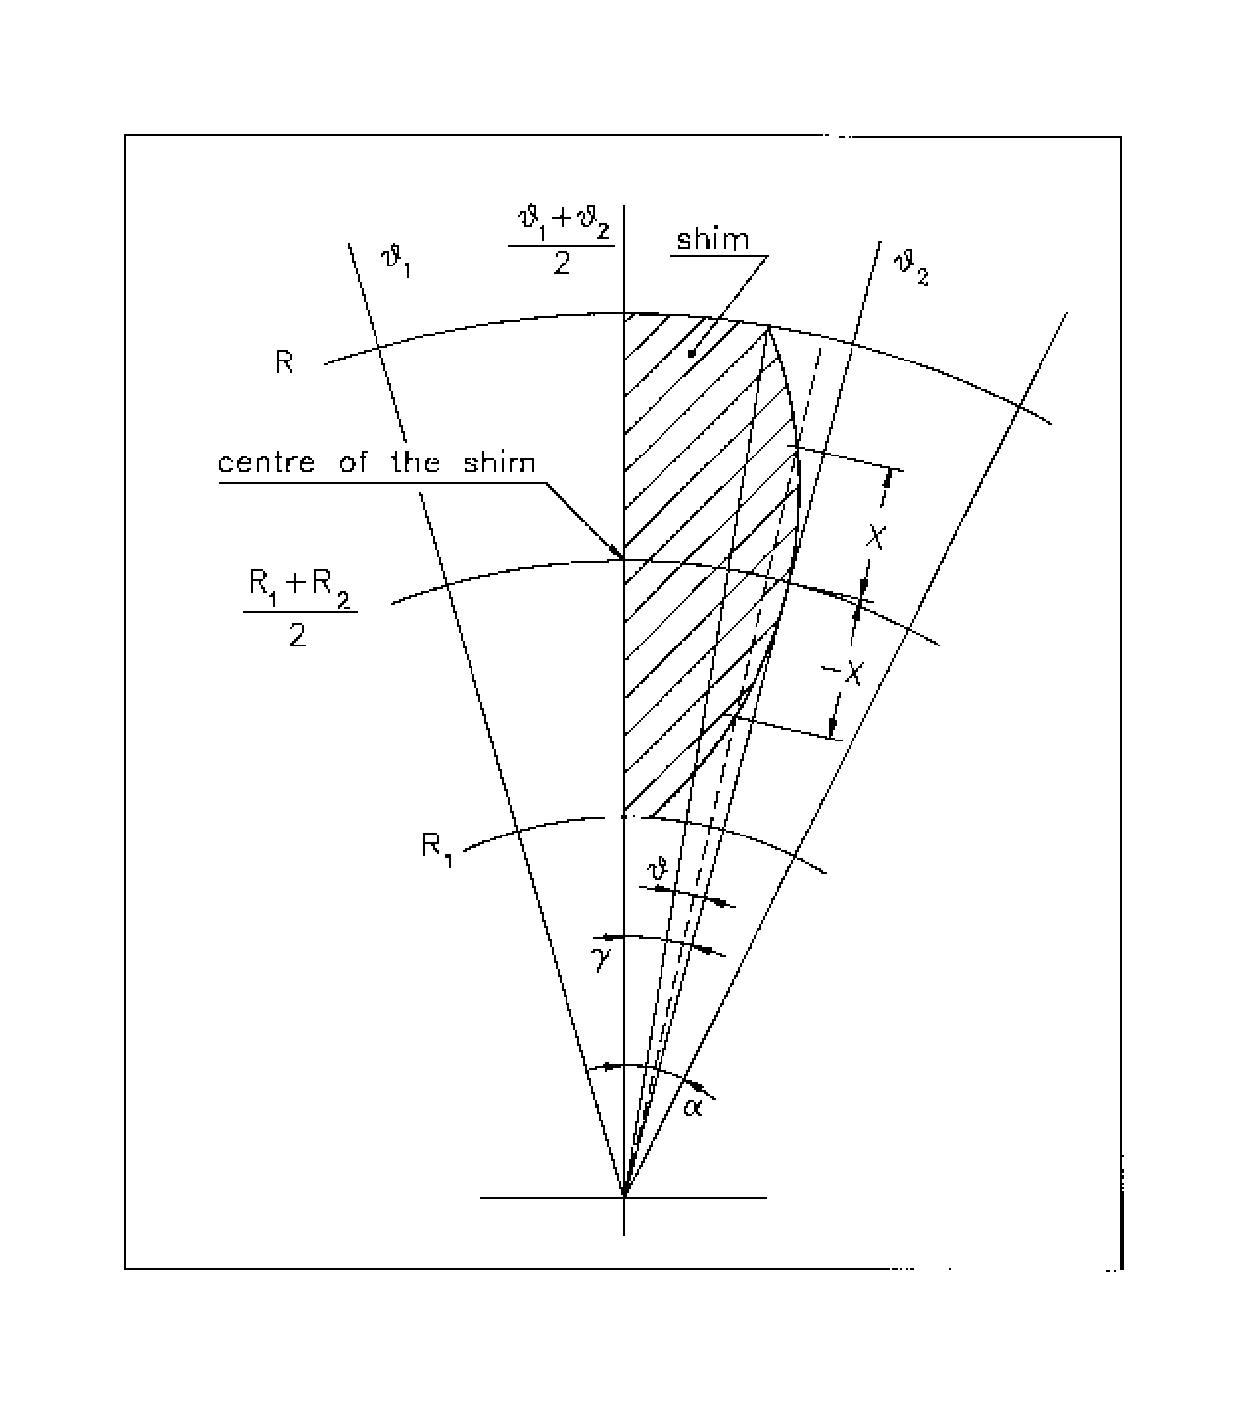
\includegraphics[height=10cm]{Fig13.ps}}
{\setlength{\captionwidth}{10cm}
\hangcaption[Fig13]{\label{fig13}A second order profile shim.  The shim is centered at 
$ \dfrac{(R_1+R_2) }{ 2} $ and $ \dfrac{(\theta_ 1+\theta_ 2) }{ 2} $.}   }
\end{figure}




\newpage

\subsubsection*{AUTOREF~: \AUTOREFTitl}\label{AUTOREF}\index{AUTOREF|textbf} 
\medskip

\textsl{AUTOREF} positions the new reference frame following four different options (apart from  $\mathbf{I = 0}$ 
which is just an ``off'' switch)~:
\bigskip

\noindent\textbf{If} $\mathbf{I = 1}$, \textsl{AUTOREF} is equivalent to 

$$ \text{\textsl{CHANGREF}} \lbrack XCE=0, YCE=Y(1), ALE=T(1)\rbrack $$
\index{CHANGREF}%
 so that the new reference frame is at the exit of the last element,
with particle~1 at the origin with its horizontal angle set to $ T=0$.   

\bigskip

\noindent\textbf{If} $\mathbf{I=2}$, it is equivalent to

$$ \text{\textsl{CHANGREF}} \lbrack XW, YW, T(1)\rbrack $$
%
 so that the new reference frame is at the position $ (XW, YW) $ of
the waist (calculated automatically in the same way as for 
\textsl{IMAGE\index{IMAGE}}) of the three rays number 1, 4 and 5 (compatible for instance
with \textsl{OBJET\index{OBJET}}, \textsl{KOBJ}  =  5, 6,  together with the 
use of \textsl{MATRIX})\index{MATRIX} while $T(1)$, the horizontal angle of particle number $I1$,  is set to zero.  

\bigskip

\noindent\textbf{If} $\mathbf{I=3}$,  it is equivalent to 

$$\text{\textsl{CHANGREF}} \lbrack XW,YW,T(I1)\rbrack $$
%
 so that the new reference frame is at the position $ (XW, YW) $ of
the waist (calculated automatically in the same way as for 
\textsl{IMAGE}) of the three rays number I1, I2 and I3 specified as data,  while $T(I1)$ is set to zero.
 

\bigskip

\noindent\textbf{If} $\mathbf{I=4}$~: provided \textsl{XCE, YCE, ALE}, 
 the beam is moved by $XCE$ and then centered on \textsl{YCE, ALE}. 
 


\newpage


\subsubsection*{BEAMBEAM~: \BEAMBEAMTitl}\label{BEAMBEAM}  \index{BEAMBEAM|textbf}
 \index{beam-beam spin kick} \index{spin kick, beam-beam}
\medskip

\textsl{BEAMBEAM} is a beam-beam lens simulation, a point transform~\cite{BBSW}. 

\medskip 

\noindent Upon option using \textsl{SPNTRK}, 
\textsl{BEAMBEAM} will include spin kicks, after  modelling as described in Ref.~\cite{YKBatyginSpin}. 



\newpage


\subsubsection*{BEND~: \BENDTitl}\label{BEND}  \index{BEND|textbf}
\medskip

\textsl{BEND}  is one of  several keywords available for the
simulation of dipole magnets. It presents the interest of easy handling, and is well adapted for 
the simulation of synchrotron dipoles and such other regular dipoles as sector magnets with wedge 
angles. 

\bigskip

\noindent The field in \textsl{BEND}  is defined in a Cartesian coordinate frame (unlike for instance \textsl{DIPOLE[S]} 
that uses a polar frame).  As a consequence, having particle coordinates at entrance  or exit of the magnet 
referring to the  curved  main direction of motion may 
require using \textsl{KPOS}, in particular \textsl{KPOS=3}  (in a circular machine cell for instance, 
see section~\ref{sec4.6.2}, p.~\pageref{sec4.6.2}). 

\bigskip

\noindent The dipole simulation accounts for the magnet geometrical length $ \XL $, for a possible 
 skew angle (X-rotation, useful for obtaining vertical deviation magnet), and for the 
field $ B1 $  such that   in absence of fringe field the deviation $\theta$ satisfies 
$ \XL = 2 \dfrac{\BORO}{B1} \sin \theta/2$. 

\bigskip

\noindent Then follows the description of the entrance and exit EFB's and
fringe fields.       The wedge angles $W_E $ 
(entrance) and $W_S $ (exit) are defined with respect to the sector angle, 
with the signs as described in Fig.~\ref{fig14}.  
Within a distance $ \pm X_E(\pm X_S) $ on both sides of the entrance (exit) EFB, 
the fringe field model is used (same as for \textsl{QUADRUPO}, 
Fig.~\ref{fig27}, p.~\pageref{fig27})~; elsewhere, the field is supposed to be uniform. 

\bigskip

\noindent If $\lambda_{E} $ (resp. $\lambda_{S} $) is zero sharp edge field model is assumed at entrance 
(resp. exit) of the magnet and $X_E$ (resp. $X_S$) is forced to zero.  In this case, the wedge angle vertical first order 
focusing effect (if $\vec  B1$ is non zero) is simulated at magnet entrance and exit by a kick 
$P_2 = P_1 - Z_1 \tan (\epsilon / \rho)$ applied to each particle ($P_1$, $P_2$ are the vertical angles 
upstream and downstream the EFB, $Z_1$ the vertical particle position at the EFB, $\rho$ the local horizontal 
bending radius and $\epsilon$ the wedge angle experienced by the particle~; $\epsilon$ depends on the horizontal angle T).


\bigskip

\noindent Magnet (mis-)alignment is assured by \textsl{KPOS}. 
\textsl{KPOS} also  allows some degrees of automatic alignment useful for periodic structures (section~\ref{sec4.6.2}).

\vfill
%%%%%%%%%%%%%%%figure%%%%%%%%%%%%%%
\begin{figure}[H]
  %\vspace{12 truecm}
  %%%Figure 14
%  \centerline{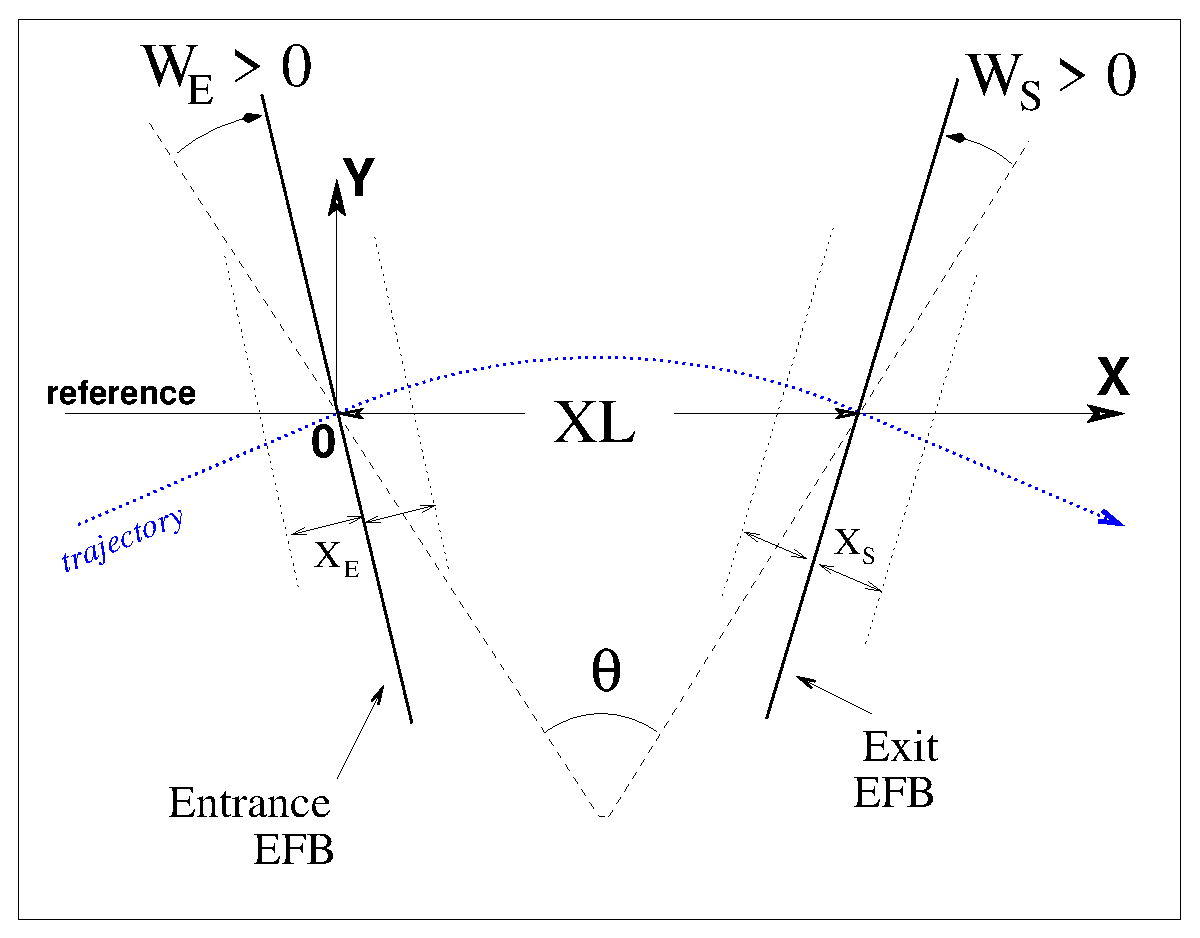
\includegraphics[height=12cm,angle=-90]{Fig14.ps}}
  \centerline{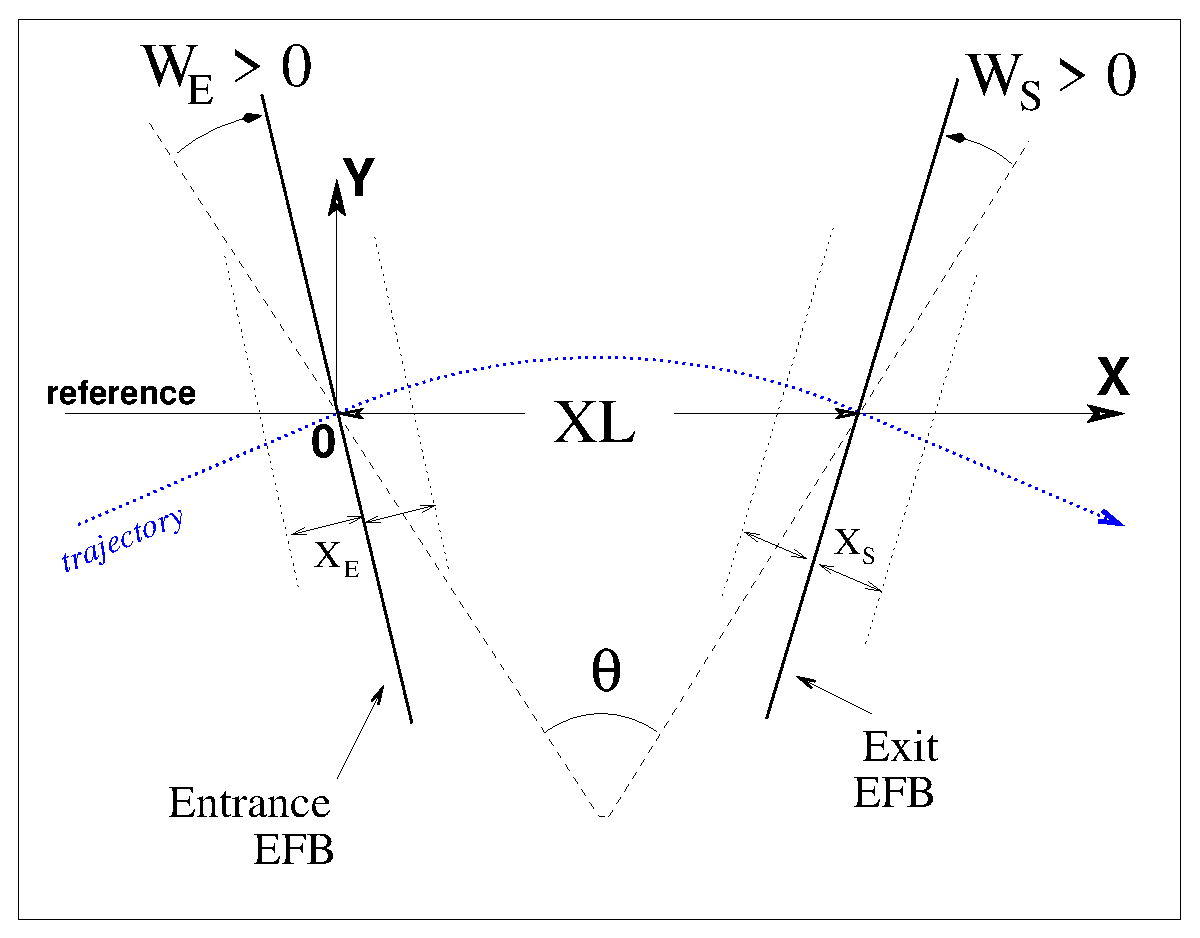
\includegraphics[height=8cm]{Fig14.eps}}
  {\setlength{\captionwidth}{12cm}
	\hangcaption[Fig14]{\label{fig14}
               \CapBEND
    } }
\end{figure}

\vfill
\newpage


\subsubsection*{BREVOL~: \BREVOLTitl} \label{BREVOL}\index{BREVOL|textbf}
\medskip

\textsl{BREVOL}  reads a 1-D axial field map from a storage data file,
whose content must match the following \FORTRAN\ reading sequence (possible FORMAT updates are to be found in \texttt{fmapw.f}).   

\bigskip


{\footnotesize
\begin{verbatim}
	      OPEN (UNIT = NL, FILE = FNAME, STATUS = `OLD' [,FORM='UNFORMATTED'])
	      DO 1 I = 1, IX
	        IF (BINARY) THEN 
	              READ(NL) X(I), BX(I)
	        ELSE
	              READ(NL,*) X(I), BX(I)
	        ENDIF
	1     CONTINUE
\end{verbatim}}
\medskip

\noindent where $\IX$ is the number of nodes along the (symmetry) $X$-axis, $X(I)$
their coordinates, and $\BX(I)$ are the values of the $X$ component of the field. $\BX$ is 
normalized with \textsl{BNORM} factor prior to ray-tracing, as well  X is normalized with 
 the coefficient  \textsl{XNORM}  (useful to convert to centimeters, the working units in  \zgoubi). 
For binary files, \textsl{FNAME} must begin with \mbox{`B\_ '} or  \mbox{`b\_ '}, 
a flag `BINARY' will thus be set to `.TRUE.' by the \FORTRAN.  

\bigskip

\noindent $X$-cylindrical symmetry is assumed, resulting in $BY$ and $BZ$ taken to 
be zero on axis. $ \vec {B} {(X,Y,Z)} $ and its derivatives along a
particle trajectory are calculated by means of a 5-point polynomial interpolation followed by second 
order off-axis  extrapolation (see sections~\ref{sec2.3.1},~\ref{sec2.4.1}).  
\bigskip

\noindent Entrance and/or exit integration boundaries may be defined in the same way 
as in \textsl{CARTEMES\index{CARTEMES}} by means of the flag $ID$ and coefficients
$A$, $B$, $C$, etc. 

\newpage

\subsubsection*{CARTEMES~: \CARTEMESTitl}\label{CARTEMES}\index{CARTEMES|textbf}
\medskip

\textsl{CARTEMES}  was originally dedicated to the reading 
and processing of the measured median plane field maps of the QDD spectrometer  SPES2 at Saclay, 
assuming mid-plane dipole symmetry.  However, it can be
used for the reading of any 2-D median plane maps, provided that the format of the
field data storage file fits the following \FORTRAN\ sequence 


{\footnotesize
\begin{verbatim}
	      OPEN (UNIT = NL, FILE = FNAME, STATUS = `OLD' [,FORM='UNFORMATTED'])
              IF (BINARY) THEN 
                READ(NL) (Y(J), J=1, JY)
              ELSE
                READ(NL,FMT='(10F8.2)') (Y(J), J=1, JY)
              ENDIF
              DO 1 I=1, IX
	        IF (BINARY) THEN 
	          READ(NL) X(I), (BMES(I,J), J=1, JY)
	        ELSE
	          READ(NL,FMT='(10F8.1)') X(I), (BMES(I,J), J=1, JY) 
                ENDIF
        1     CONTINUE
\end{verbatim}}

\noindent where, $IX$  and $JY$  are the number of longitudinal
and transverse horizontal nodes of the uniform mesh, and $X(I)$, $Y(J)$ their coordinates.  
\textsl{FNAME} 
 is the name of the file containing the field data. For binary files, \textsl{FNAME} must begin with
\mbox{`B\_ '} or \mbox{`b\_'},  a flag `BINARY' will thus be set to `.TRUE.' by the \FORTRAN.  
\bigskip

\noindent The measured field \textsl{BMES} is normalized with \textsl{BNORM},

$$ B(I,J) = \text{\textsl{BMES}}(I,J) \times  \text{\textsl{BNORM}} $$

\noindent As well the longitudinal coordinate  X is normalized with 
a  \textsl{XNORM} coefficient (useful to convert to centimeters, the working units in  \zgoubi). 

\noindent The vector field, $ \vec  B $, and its derivatives out of the median
plane are calculated by means of a second or fourth order polynomial 
interpolation, depending on 
the value of the parameter \textsl{IORDRE\index{IORDRE}} (\textsl{IORDRE} = 2, 25 or 4, 
see section~\ref{sec2.4.2}). 
\bigskip

\noindent In case a particle  exits the mesh, its \IEX\index{IEX@{\IEX}} flag is set to $-1$ (see section~\ref{sec4.6.6}, 
p.~\pageref{sec4.6.6}), however it is still tracked with the field being {\it extrapolated} from 
the closest  nodes of the mesh. Note that such extrapolation process may induce erratic behavior if the distance from the mesh gets 
too large. 

\bigskip

\noindent Entrance and/or exit integration boundaries can be defined with 
the flag $ID$\index{ID@{\textsl{ID}}|textbf}, as follows (Fig.~\ref{fig15}).
\bigskip

\noindent \textbf{If  $\mathbf{ID = 1}$~:} the integration in the field 
is terminated on a boundary with equation $A'X + B'Y + C'=0 $, and 
then the trajectories are extrapolated linearly onto the exit border of the map.

\medskip

\noindent \textbf{If  $\mathbf{ID = -1}$~:} an entrance boundary is 
defined, with equation $A'X + B'Y + C'=0 $, up to which  trajectories are 
first extrapolated linearly from the map entrance border, prior to being 
integrated in the field.

\medskip

\noindent \textbf{If  $\mathbf{ID \geq 2}$~:} one entrance boundary, and 
$ID-1$~exit boundaries are defined, as above. The integration in the 
field terminates on the last ($ID - 1$) exit boundary. No extrapolation onto 
the map exit  border is performed in this case.

\newpage

%%%%%%%%%%%%%%figure%%%%%%%%%%%%%%
\begin{figure}[H]
%\vspace{19 truecm}
%%%Figure 15
\centerline{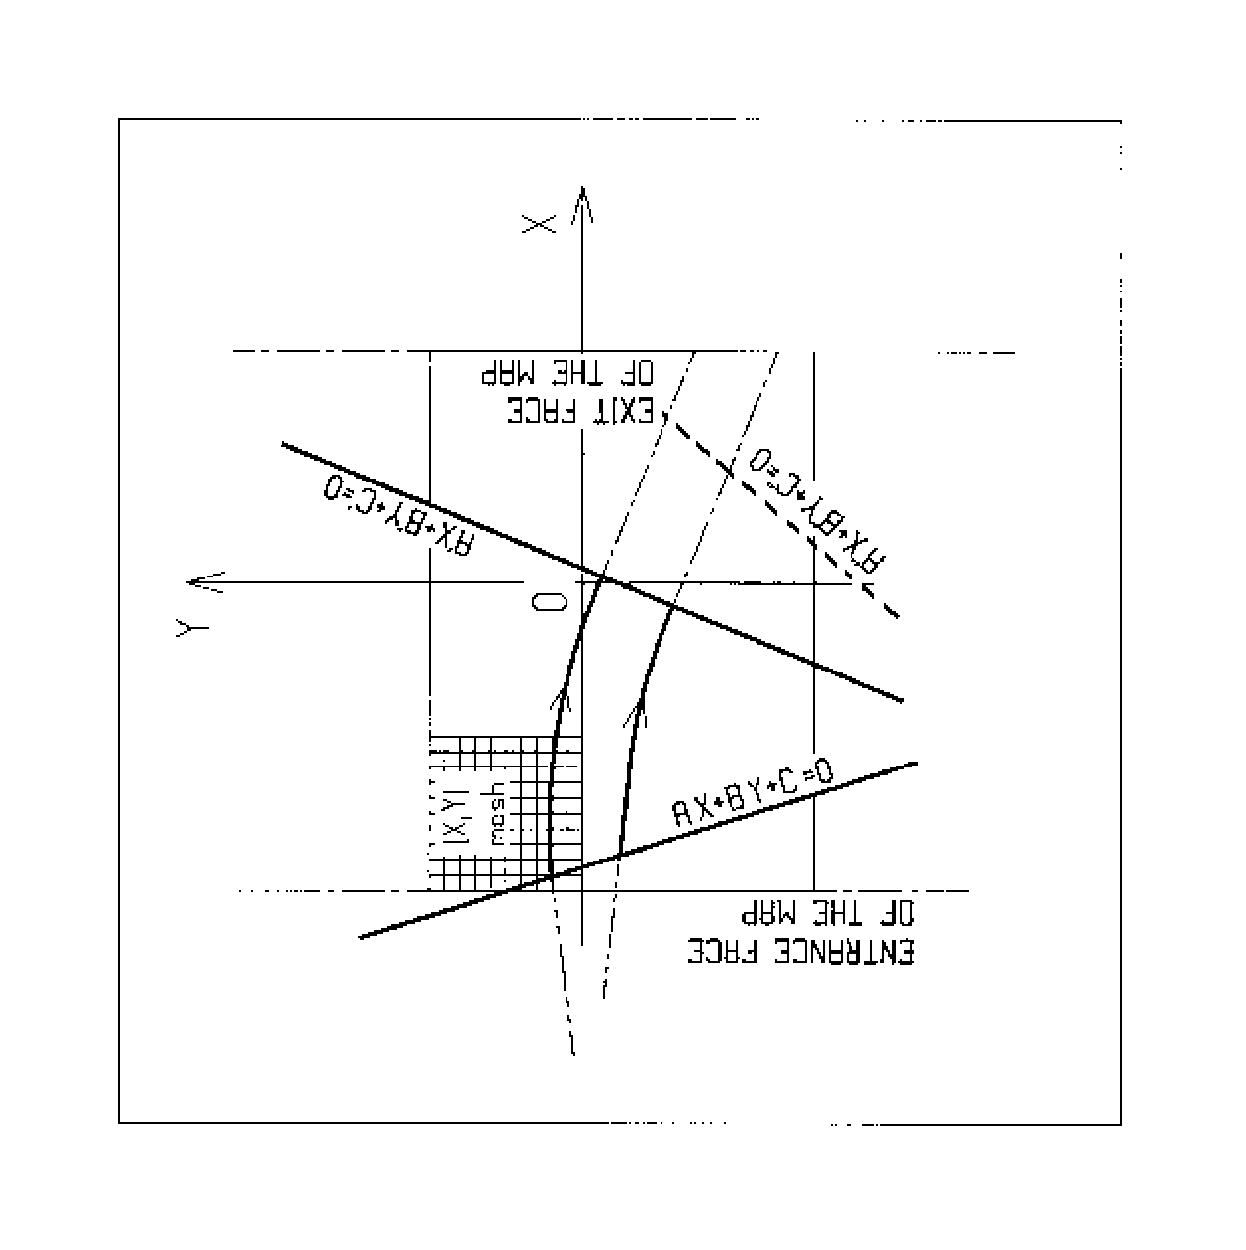
\includegraphics[height=15cm,angle=-90]{Fig15.ps}}
{\setlength{\captionwidth}{16cm}
\hangcaption[Fig15]{\label{fig15}$OXY $ is the coordinate system of the mesh.
Integration boundaries may be defined, using $ ID\not= 0 $~: particle coordinates are
extrapolated linearly from the entrance face of the map, onto the boundary 
$A'X+B'Y+C'=0$~; after ray-tracing inside the 
map and terminating on the boundary $AX+BY+C=0$, coordinates are
extrapolated linearly onto the exit face of the map if $ID=2$, or 
 terminated on the last ($ID-1$) boundary if $ID >2$.}
}
\end{figure}
\vfill
\newpage

\subsubsection*{CAVITE~: \CAVITETitl}  \label{CAVITE}\index{CAVITE|textbf}
\index{acceleration}\index{synchrotron motion}
\medskip

\textsl{CAVITE}  provides a  simulation of a (zero length)
accelerating cavity~; it can be used in conjunction with  keywords \REBELOTE\index{REBELOTE} 
and \textsl{SCALING} for 
the simulation of multi-turn\index{multi-turn tracking} tracking with synchrotron or 
fixed field (FFAG, cyclotron) \index{FFAG} \index{cyclotron} acceleration (see section~\ref{sec4.6.4}). 
It must be preceded by \textsl{PARTICUL} for the definition 
of mass ~$ M $ and charge~$ q$.   

\bigskip

\noindent A major effect of \textsl{CAVITE} on optics settings is the following~:  \index{reference rigidity} 

\medskip

\noindent The reference rigidity of a problem, as used when computing optical strengths from field values, 
sections~\ref{sec2.2.1}-\ref{sec2.2.3}, 
 is specified in the object definition by \textsl{[MC]OBJET}.  However, in many 
cases -- options as described below -- that  reference rigidity will be updated upon crossing the cavity, 
by the amount of the synchronous rigidity increase as induced by the cavity, namely, 
$$B\rho_{ref} = \BORO \longrightarrow B\rho_{ref} = \BORO + \delta \Br_s$$ \index{BORO@{\BORO}$\times D_{ref}$|textbf}
Note as an illustration of the process, that, in this case, a simple way to have the 
optical elements have their \textsl{strengths} maintained constant is to 
use \textsl{SCALING} with the option $\NTIM=-1$.

\bigskip

\noindent \textbf{If $\mathbf{IOPT  =  0}$~:}   \textsl{CAVITE} is switched off.  
\bigskip

\noindent\textbf{If $\mathbf{IOPT  =  1}$~:}  \textsl{CAVITE} simulates the RF~cavity of a 
synchrotron accelerator~: 
the periodic motion over $IP  = 1$, \textsl{NPASS} + 1 \index{NPASS}
turns (passes through the structure) is obtained using the keyword \textsl{REBELOTE\index{REBELOTE}}, option 
\mbox{K  =  99},  while  RF  and optical elements  time dependent functions are simulated by means of
\textsl{SCALING} -- see section~\ref{sec4.6.4}. 
 \textsl{CAVITE} may conveniently be located  \textsl{at the end} of the optical 
structure, otherwise its phasing has to be indicated. 
The synchrotron motion of any of the 
\IMAX\index{IMAX@{\IMAX}} particles of a beam is obtained from  the following mapping 

$$ \left\{ 
\begin{array}{l}
	\phi_ 2-\phi_ 1= 2\pi \, f_{RF}\, 
	     \left(  \dfrac{\ell}{ \beta c} - \dfrac{\mathcal{L} }{ \beta_sc} \right) \\
	W_2-W_1 = q\hat  V\, \sin\phi_ 1  
\end{array}
\right. $$
%
 where
  
{\renewcommand{\arraystretch}{1}
 \begin{tabular}{>{$}l<{$}!{=}l}
	\phi        &  RF phase~; $\phi_ 2-\phi_ 1=$ variation  of $\phi$ between two  traversals\\
	W           &   kinetic  energy~;  $W_2-W_1=$ energy  gain  at  a traversal  of \textsl{CAVITE}\\
	\mathcal{L} & length  of  the  synchronous  closed orbit\index{closed orbit}  (to  be  calculated  by  prior 
	              ray-tracing,   \index{closed orbit}    \\
	 \multicolumn{1}{c}{  }           & see  the  bottom  NOTE) \\
	\ell        &  orbit length  of  the  particle  between  two  traversals\\
	\beta_ sc   &  velocity  of  the (virtual)  synchronous  particle\\
	\beta c     &  velocity  of  the  particle \\
	\hat  V     &  peak RF voltage\\
	q           &  particle  electric  charge.   
 \end{tabular}}
\bigskip

\noindent The RF frequency $ f_{RF} $ is a multiple of the synchronous 
revolution frequency, and is obtained from the input data, following 

$$ f_{RF} = \dfrac{hc }{\mathcal{L}}\, \dfrac{q(\Br )_s }{ \sqrt{q^2(\Br)^2_s+(Mc)^2}} $$
%
 where
  
 \begin{tabular}{l!{=}l}
   $h$ & harmonic  number  of  the  R.F\\
   $M$ &  mass  of  the  particle \\
   $c$ & velocity  of light.
  \end{tabular}
\bigskip

\noindent The current rigidity $ (\Br)_s $ of the synchronous particle is
obtained from the timing law specified by means of \textsl{SCALING} following 
$ (\Br)_s= \BORO\cdot \text{\textsl{SCALE(TIMING)}} $\index{BORO@{\BORO}} 
(see  \textsl{SCALING}  for the meaning and calculation of the scale 
factor \textsl{SCALE(TIMING)}). \textsl{If \textsl{SCALING\index{SCALING}} is 
not used, $ (\Br )_s $ is assumed to keep the constant value \BORO\
} as given in the object description (see \textsl{OBJET\index{OBJET}} for instance). \

\noindent The velocity $ \beta c $ of a particle is calculated from its
current rigidity

$$ \beta  = \dfrac{q(\Br ) }{ \sqrt{ q^2(\Br )^2+(Mc)^2}} $$
%
 The velocity $ \beta_ sc $ of the synchronous particle is obtained
in the same way from

$$ \beta_ s = \dfrac{q(\Br )_s }{ \sqrt{ q^2(\Br )^2_s + (Mc)^2}} $$
%
 The kinetic energies and rigidities involved in these formulae are related by

$$ q(\Br ) = \sqrt{ W(W+2Mc^2)} $$
%
 Finally, the initial conditions for the mapping, at the first 
turn, are the following  
\begin{itemize}
\item[-] For the (virtual) synchronous particle
%
\begin{align*}
	\phi_ 1 &  = \phi_ s = \text{synchronous phase}  \\
	(\Br )_{1s} & = \BORO  
\end{align*}

\item[-] For any of the $ I=1$,  \IMAX\index{IMAX@{\IMAX}}  particles of the beam 
%
\begin{align*}
	\phi_{1I} & = \phi_ s = \text{synchronous  phase} \\
	(\Br )_{1I} & =\BORO \ast  D_I
\end{align*}
%
\noindent where the quantities \BORO\ and $ D_I $ are given in the object description. 
\end{itemize}

\paragraph{Calculation of the Coordinates} 

\noindent Let   $ p_I= \left[p^2_{\XI}+p^2_{YI}+p^2_{ZI} \right]^{1/2} $ be the momentum of particle 
$ I $ at the exit of the cavity, while   %%%%% adjustment cesure peu satisfaisant !!
$ p_{I_0}= \left[p^2_{\XI_0}+p^2_{YI_0} + p^2_{ZI_0}\right]^{1/2} $ is its 
momentum at the entrance. The kick in momentum is assumed to be 
fully longitudinal, resulting in the following relations between 
the coordinates at the entrance (denoted by the index zero) and at the exit 

 \begin{align*}
	 p_{\XI} 
	      & = \left[p^2_I-(p^2_{I_0}-p^2_{\XI_0}) \right]^{1/2} \\
	p_{YI} & = p_{YI_0},\quad \text{and} \quad  p_{ZI}= p_{ZI_0} \quad\text{(longitudinal  kick)} \\ 
	X_I &  = X_{I_0},\quad Y_I=Y_{I_0}\quad  \text{and} 
	        \quad Z_I=Z_{I_0} \quad\text{(zero  length cavity)}   
 \end{align*}
%
and for the angles (see Fig.~\ref{fig1})  
%
\begin{equation*}
	\left. 
	\begin{aligned}
		T_I & =  \text{Atg} \left( \dfrac{p_{YI}}{ p_{\XI}} \right) \\
		P_I &  =  \text{Atg} \left(\dfrac{P_{ZI}}{(p^2_{\XI}+p^2_{YI})^{1/2}} \right) 
	\end{aligned}
	 \right\rbrace \quad \text{(damping  of the  transverse  motion)}
\end{equation*}  
%\vfill\eject

\noindent\textbf{If $\mathbf{IOPT  =  2~:}$} the same simulation of a synchrotron RF cavity 
as for $\mathbf{IOPT  =  1}$ is performed, except that the keyword 
\textsl{SCALING\index{SCALING}} (family \textsl{CAVITE\index{CAVITE}}) is not taken into 
account in this option~: the increase in kinetic energy at each traversal, 
for the synchronous particle, is

$$ \Delta W_s= q\hat  V \,\sin\phi_ s $$
%
where the synchronous phase $ \phi_ s $ is given in the input data.
From this, the calculation of the law $ (\Br )_s $ and the RF frequency 
$f_{RF} $ follows, according to the formulae given in the \mbox{\textsl{IOPT}  =  1} case. 

\bigskip

\noindent\textbf{If $\mathbf{IOPT  =  3}$~:} sine RF law, acceleration without synchrotron motion. 
Any particle will be given a kick

$$ \Delta W = q\hat  V\, \sin\phi_ s $$
%
where $ \hat  V $ and $ \phi_ s $ are input data.  

\bigskip

\noindent\textbf{If $\mathbf{IOPT  =  6}$~:}  
allows reading the RF frequency and/or phase law from an external file (wih name normally ``zgoubi.freqLaw.In''). 
See routines \texttt{cavite.f} and \texttt{scalin.f} for details
Was first used for  acceleration  in scaling FFAG~\cite{reportNIMFFAGSPI}. \index{FFAG}  


\bigskip

\noindent\textbf{If $\mathbf{IOPT  =  7}$~:} fixed frequency RF, quasi- or isochronous acceleration. Was 
first used for quasi-isochronous, fixed frequency acceleration in the EMMA prototype 
linear FFAG~\cite{repDapniaEMMA,EMMAIPAC10}. 

\noindent Can be used for  cyclotron \index{cyclotron} acceleration. 



\bigskip

\noindent {\bf NOTE. Calculation of the closed orbit~:}     \index{closed orbit}  

\medskip

\noindent Due to possible dipole type of optical defects (\eg, fringe fields, straight axis 
combined function dipoles), the closed orbit may not 
coincide with the ideal axis of the optical elements (hence it will be almost everywhere non-zero). One way to 
calculate it at the beginning of the structure (\emph{i.e.}, where the 
initial particle coordinates are defined) is to ray-trace 
a single particle over a sufficiently large number of turns, 
starting with   initial conditions  taken near the reference orbit, so as to 
obtain  statistically well-defined transverse phase-space ellipses. The 
local closed orbit  coincides with the 
coordinates $ Y_c $,  $ T_c $, $ Z_c $,  $ P_c $ of the center of the ellipses. 
A few iterations are usually sufficient (avoid near-integer tunes) to ensure accuracy.  Next, 
ray-tracing over one turn a particle starting with the initial condition 
($Y_c $, $ T_c $, $ Z_c$, $P_c$)  will provide the entire closed orbit, and as a sub-product its   length $\mathcal{L}$ 
(the $ F(6,1) $ coordinate in the \FORTRAN). 

\newpage

\subsubsection*{CHAMBR~:  \CHAMBRTitl}\label{CHAMBR}\index{CHAMBR|textbf} 
\medskip

\textsl{CHAMBR} causes the identification, counting and stopping of 
particles that reach the 
transverse limits of the vacuum chamber.  The chamber can be either rectangular 
(\textsl{IFORM} = 1) or elliptic (\textsl{IFORM} = 2). The chamber is centered
at $ \YC$, $\ZC $ and has transverse dimensions $\pm YL $ and  
$\pm  ZL $ such that any particle will be stopped\index{stopped particles} if its coordinates $ Y,Z $ satisfy 

\begin{align*}
	(Y-\YC)^2\geq  YL^2  \text{ or }   (Z-\ZC)^2 \geq  ZL^2 
	   &   \quad \text{if}\quad  \text{\textsl{IFORM}}=1  \\
	\dfrac{ (Y-\YC)^2 }{ YL^2} + \dfrac{(Z-\ZC)^2 }{ ZL^2} \geq 1  
	  &   \quad \text{if}\quad  \text{\textsl{IFORM}}=2  
\end{align*}

\noindent The conditions introduced with \textsl{CHAMBR\index{CHAMBR}} are valid
along  the optical structure until the next occurrence  of the keyword \textsl{CHAMBR}.  Then, if
$ \IL=1 $ the aperture is possibly modified by introducing new values of $ \YC$,  $ \ZC$, 
 $YL $ and $ ZL $, or, if $ \IL=2 $ the chamber ends and information is 
printed concerning those particles that have been stopped.  
\bigskip

\noindent The testing is done in optical elements at each integration step, between the
\textsl{EFB}'s. For instance, in \textsl{QUADRUPO\index{QUADRUPO}} there will be 
no testing from $-X_E $ to 0 and 
from $ \XL $ to $ \XL+X_S $, but only from 0  to $ \XL $~;  in \textsl{DIPOLE\index{DIPOLE}}, there is no 
testing as long as the \textsl{ENTRANCE EFB} is not reached, and testing is stopped as 
soon as the \textsl{EXIT} or \textsl{LATERAL EFB}'s are passed.  
\bigskip

\noindent In optical elements defined in polar coordinates,  $ Y $  stands for the radial
coordinate (\emph{e.g.}, \textsl{DIPOLE\index{DIPOLE}}, see Figs.~\ref{fig3}C, p.~\pageref{fig3}, and~\ref{fig9}, 
p.~\pageref{fig9}).  
 Thus, centering \textsl{CHAMBR\index{CHAMBR}} at $ \\YC=\RM $ simulates a chamber curved with radius 
 $ \RM $, and having a radial acceptance $ \RM \pm \YL $.  In  \textsl{DRIFT}, the testing  is done 
 at the beginning and at the end, and only for positive drifts.  There 
is no testing in \textsl{CHANGREF\index{CHANGREF}}.  
\bigskip

\noindent When a particle is stopped\index{stopped particles}, its index 
\IEX\index{IEX@{\IEX}}  (see \textsl{OBJET\index{OBJET}} and 
section~\ref{sec4.6.6}) is set to the value -4, and its actual path length is stored in the array 
\textsl{SORT} for possible further use. 




\newpage

\subsubsection*{CHANGREF~: \CHANGREFTitl} \label{CHANGREF}\index{CHANGREF|textbf}
\medskip 

\noindent \CHANGREF\     \index{CHANGREF}   
transports  particles from a reference plane  $(O,Y,Z)$  at path distance $S$, to a new one by a combination of 
translations and/or rotations.  It essentially aims at positioning optical elements with respect 
to one another, 
as setting a reference frame at the entrance
or exit of field maps, or to simulate misalignments (see also  \textsl{KPOS} option).  
 \CHANGREF\      can be placed anywhere in a structure. 

\medskip

\noindent  Spin tracking\index{spin tracking}, 
particle decay and gas-scattering are taken into account in  \CHANGREF. 
Energy loss by synchrotron radiation (\textsl{SRLOSS} keyword) is not. 

\medskip

\noindent There are two ``styles'' of \CHANGREF, as follows.

\bigskip

\noindent \textbf{ The ``old style'' \CHANGREF}~    \label{CHANGREFOld}  \index{CHANGREF\ ``Old Style''}
requires the three data $\XCE, ~ \YCE, ~ \ALE$ and then 
 gets the  new particle coordinates  $ Y_2$,  $ T_2$,  $ Z_2$, 
$ P_2 $  and path length $ S_2 $  from the old ones  $ Y_1$,   
$ T_1$,  $ Z_1$,  $ P_1 $ and $ S_1 $ using

\begin{figure}[h]
\begin{minipage}{.4\linewidth}
\begin{align*}
	T_2 &=  T_1- \text{\textsl{ALE}} \\
	Y_2 & = \dfrac{ (Y_1-YCE) \cos T_1+XCE \sin T_1}{\cos  T_2} \\
	DL^2 & =(XCE-Y_2 \sin \text{\textsl{ALE}})^2 
	         +(YCE-Y_1+Y_2 \cos \text{\textsl{ALE}})^2 \\
	Z_2  & = Z_1+DL\mathrm{tg} P_1 \\ 
	S_2 & = S_1+ \dfrac{DL }{ \cos P_1} \\
	P_2 & = P_1  
\end{align*}
\end{minipage}
\begin{minipage}{.5\linewidth}
\centerline{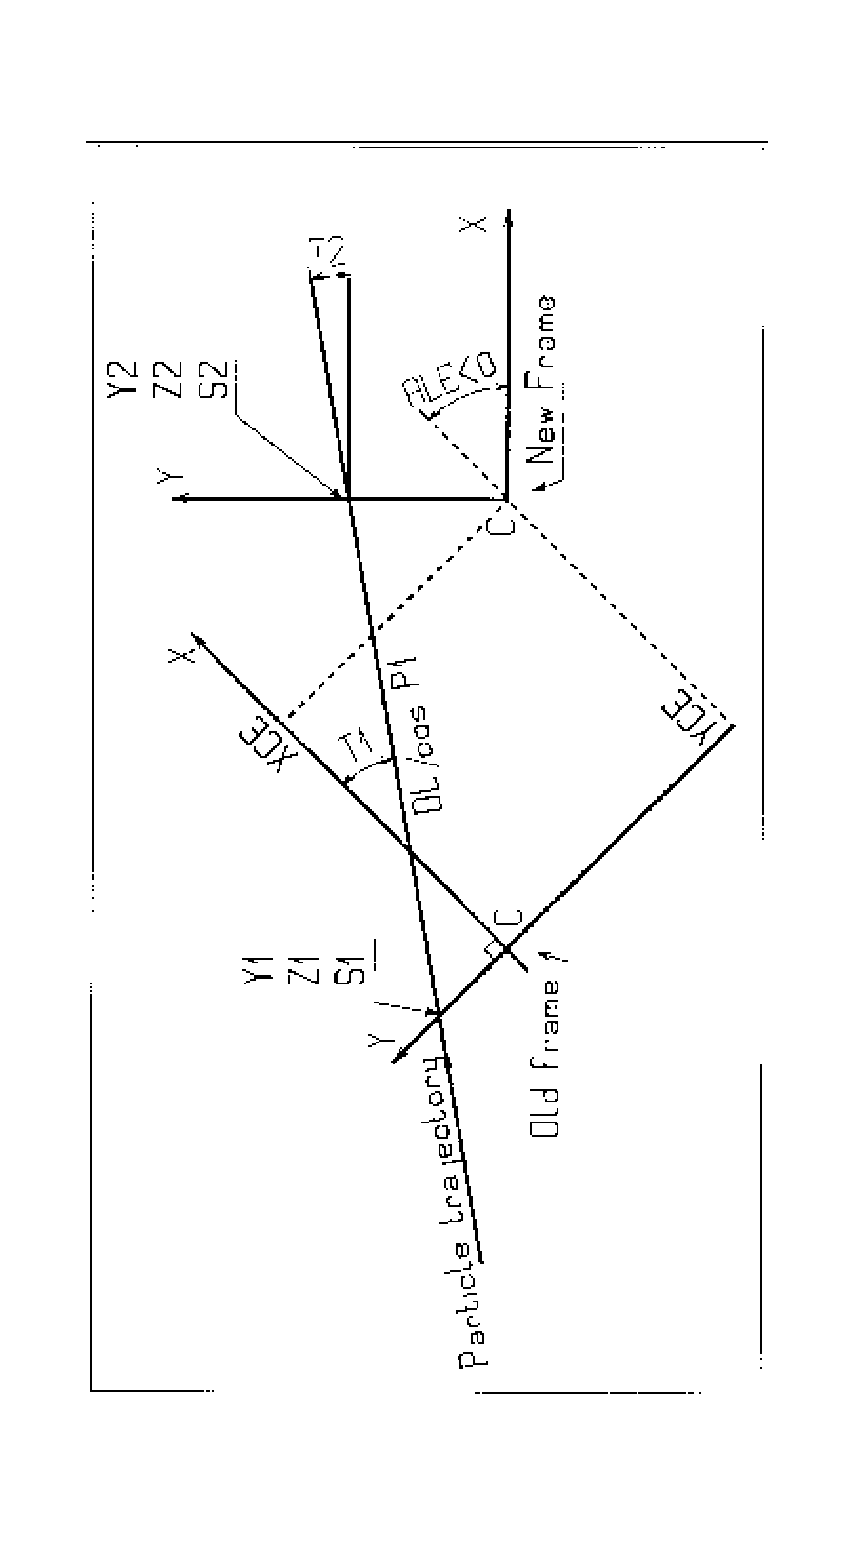
\includegraphics[height=8.5cm,angle=-90]{FigCHAREFa.eps}}
\hangcaption{\label{FigCHAREFa}Scheme of the \CHANGREF\ procedure. }
\end{minipage}
\end{figure}

\noindent where, $ XCE $ and $ YCE $ are shifts in the horizontal plane along, respectively, 
$ X$- and $ Y$-axis, and \textsl{ALE}  is a rotation around the $ Z$-axis. $ DL $
is given the sign of $ XCE-Y_2 \sin(\text{\textsl{ALE}})$.  


%%%%%%%%%%%%%%figure%%%%%%%%%%%%%%
%\begin{figure}[H]
%%\vspace{10.5 truecm}
%%%%Figure 16
%\centerline{\includegraphics[height=15cm,angle=-90]{Fig16.ps}}
%\hangcaption{\label{fig16}Scheme of the \CHANGREF\ procedure. }
%\end{figure}

\medskip


\noindent The example below shows the use of  \CHANGREF\ for the symmetric positioning of 
a combined function dipole+quadrupole  magnet in a drift-bend-drift geometry with 
12.691~degrees deviation (obtained upon combined effect of  a dipole component and 
of quadrupole axis shifted 1~cm off optical axis). 

\medskip

\begin{minipage}{1.\linewidth}
\begin{minipage}{.52\linewidth}

 Zgoubi data file~: 

\footnotesize
\begin{verbatim}
Using CHANGREF, "Old style"
'OBJET'
51.71103865921708         ! Electron, Ekin=15MeV.
2
1 1                       ! One particle, with
2. 0.  0.0 0.0 0.0 1. 'R' ! Y_0=2 cm. 
1 1 1 1 1 1 1 
'MARKER'    BEG    .plt   ! Print into zgoubi.plt.
'DRIFT'                   ! 10 cm drift.
10.
'CHANGREF'  
0. 0. -6.34165            ! 1/ half Z-rotation.
'CHANGREF'  
0. 1. 0.                  ! 2/ Y-shift.
'MULTIPOL'       ! Combined function dipole + quadrupole.
   2                      ! Print into zgoubi.plt.
5  10. 2.064995867082342  2. 0. 0. 0. 0. 0. 0. 0. 0.
 0 0  5. 1.1  1.00 1.00 1.00 1.00 1.00 1. 1. 1. 1.                              
4  .1455   2.2670  -.6395  1.1558  0. 0.  0.                                    
 0 0  5. 1.1  1.00 1.00 1.00 1.00 1.00 1. 1. 1. 1.                              
4  .1455   2.2670  -.6395  1.1558  0. 0.  0.                                    
0 0 0 0 0 0 0 0 0 0
.1   step size
1  0. 0.  0.
'CHANGREF'
0. -1. -6.34165           ! 1/ Y-shift, 2/ half Z-rotate.
'DRIFT'                   ! 10 cm drift.
10.
'FAISCEAU'
'END'
\end{verbatim}
\normalsize
\end{minipage}\hspace{.05\linewidth}
\begin{minipage}{.35\linewidth}
\centerline{\includegraphics*[bbllx=20,bblly=100,bburx=567,bbury=470,width=1.\linewidth]{FigCHAREFb.eps}}

Note~: The square markers scheme the stepwise integration in case of $\pm$5~cm additional fringe field 
extent upstream and downstream of the 5~cm long multipole. 
\end{minipage}
\end{minipage}




\bigskip

\noindent \textbf{The ``new style'' \CHANGREF}~ \label{CHANGREFNew}  \index{CHANGREF\ ``New Style''} 
    allows all 6 degrees of freedom rather than just 3, namely, X-, Y-, Z-shift, X-, Y-, Z-rotation.  
In addition, \CHANGREF\  ``new style''  allows up to 9 successive such elementary transformations,  in arbitrary order. 
The ``old style'' example above is transposed into  ``new style'',  hereafter. 

\medskip

\begin{minipage}{1.\linewidth}

 Zgoubi data file~: 

\footnotesize
\begin{verbatim}
Using CHANGREF, "New Style"
'OBJET'
51.71103865921708         ! Electron, Ekin=15MeV.
2
1 1                       ! One particle, with
2. 0.  0.0 0.0 0.0 1. 'R' ! Y_0=2 cm. 
1 1 1 1 1 1 1 
'MARKER'    BEG    .plt   ! Print into zgoubi.plt.
'DRIFT'                   ! 10 cm drift.
10.
'CHANGREF'  
ZR -6.34165 YS 1.         ! 1/ half Z-rotate, 2/ Y-shift.
'MULTIPOL'       ! Combined function dipole + quadrupole.
   2                      ! Print into zgoubi.plt.
5  10. 2.064995867082342  2. 0. 0. 0. 0. 0. 0. 0. 0.
 0 0  5. 1.1  1.00 1.00 1.00 1.00 1.00 1. 1. 1. 1.                              
4  .1455   2.2670  -.6395  1.1558  0. 0.  0.                                    
 0 0  5. 1.1  1.00 1.00 1.00 1.00 1.00 1. 1. 1. 1.                              
4  .1455   2.2670  -.6395  1.1558  0. 0.  0.                                    
0 0 0 0 0 0 0 0 0 0
.1   step size
1  0. 0.  0.
'CHANGREF'
YS -1. ZR -6.34165        ! 1/ Y-shift, 2/ half Z-rotate.
'DRIFT'                   ! 10 cm drift.
10.
'FAISCEAU'
'END'
\end{verbatim}
\end{minipage}







\newpage

\subsubsection*{CIBLE or TARGET~: \CIBLETitl}
\label{CIBLE}\label{TARGET}
\index{CIBLE|textbf} \index{TARGET|textbf}
\medskip

 The reaction is $ 1+2 \longrightarrow  3+4 $ with the following parameters 
$$
\begin{array}{lllll}
	\text{Laboratory momentum} & p_1\equiv  0 &  p_2 &   p_3 &    p_4 \\
	\text{Rest mass}           &   M_1        &   M_2 & M_3 &    M_4 \\ 
	\text{Total energy in laboratory} & M_1c^2 &  W_2 &    W_3 &   W_4 
\end{array}
$$
%
 The geometry of the interaction is shown in Fig.~\ref{fig17}.   
\medskip

\noindent The angular  sampling at the exit of the target consists of the $ NT$ 
coordinates 0,  $ \pm TS$,  $ \pm 2\ast TS$...   $\pm (NT-1)\ast TS/2 $ 
in the median plane, 
and the $ NP $ coordinates 0, $ \pm PS$,  $ \pm 2\ast PS$... $ \pm (NP-1)\ast PS/2$ 
in the vertical plane.  
\medskip

\noindent The position of $ B $ downstream is deduced from that of $ A $
upstream  by a transformation equivalent to two transformations using \textsl{CHANGREF\index{CHANGREF}},
 namely
 \begin{gather*}
	 \text{\textsl{CHANGREF}}(XCE=YCE=0,\quad  \textsl{ALE}=\beta )  \\
\intertext{followed by} 
	 \text{\textsl{CHANGREF}}(XCE=YCE=0,\quad \textsl{ALE}=\theta -\beta ). 
 \end{gather*}

 
\noindent Particle  4 is discarded, while particle 3 continues. The energy
loss $ Q $ is related to the variable mass $ M_4 $ by
$$ Q=M_1+M_2-(M_3+M_4)\qquad \text{and} \qquad dQ=-dM_4 $$

\noindent The momentum sampling of particle 3 is derived from conservation of
energy and 
momentum, according to 

\begin{align*}
	M_1c^2+W_2 & =  W_3+W_4  \\
	p^2_4 & =  p^2_2 +p^2_3 -2p_2p_3 \cos (\theta -T) 
\end{align*}


%%%%%%%%%%%%%%figure%%%%%%%%%%%%%%
\begin{figure}[H]
%\vspace{17 truecm}
%%%Figure 17
\centerline{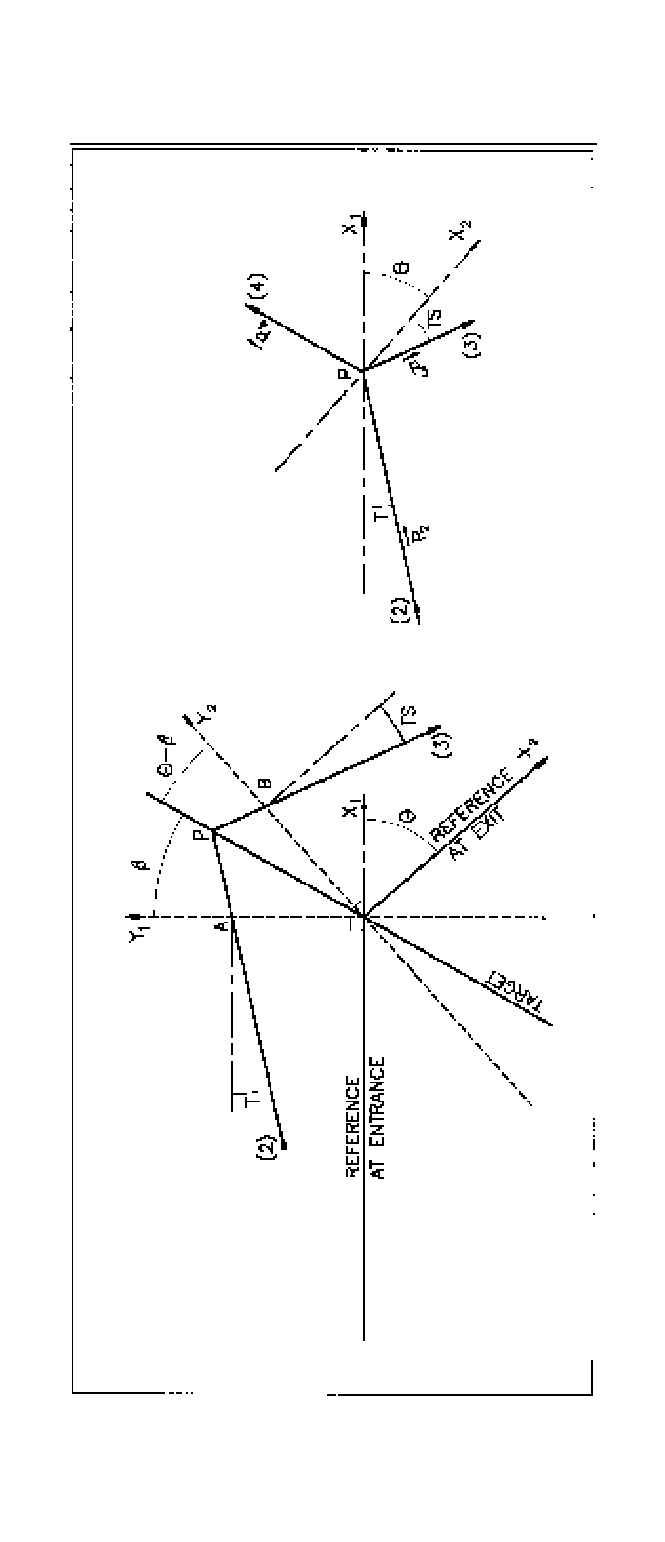
\includegraphics[height=15cm,angle=-90]{Fig17.ps}}
{\setlength{\captionwidth}{15cm}
\hangcaption[Fig17]{\label{fig17}Scheme of the principles of \textsl{CIBLE (TARGET)}\\
 $ A, T$   =   position, angle of incoming particle 2 in the entrance reference frame\\
 $P$   =   position of the interaction\\
 $B, T$   =   position, angle of the secondary particle  in the exit reference frame\\ 
 $\theta$   =   angle between entrance and exit frames\\
 $\beta$   =   tilt angle of the target}     }
\end{figure}
\vfill

\newpage

\subsubsection*{COLLIMA~: \COLLIMATitl}\label{COLLIMA}\index{COLLIMA|textbf}
\medskip

\textsl{COLLIMA}  acts as a mathematical aperture of zero length.  It causes 
the identification, counting and stopping of particles that reach the aperture limits.  

\paragraph{Physical Aperture}

\noindent A physical aperture can be either rectangular (\textsl{IFORM} = 1) or elliptic 
(\textsl{IFORM} = 2).  The collimator is centered at $ \YC$, $\ZC $ and has transverse
dimensions $\pm YL $ and $\pm ZL $ such that any particle will be
stopped\index{stopped particles} if its coordinates $Y$, $Z $ satisfy
\begin{align*}
	(Y-\YC)^2\geq  YL^2  \text{ or }   (Z-\ZC)^2 \geq  ZL^2 
	   &   \quad \text{if}\quad  \text{\textsl{IFORM}}=1  \\
	\dfrac{ (Y-\YC)^2 }{ YL^2} + \dfrac{(Z-\ZC)^2 }{ ZL^2} \geq 1  
	  &   \quad \text{if}\quad  \text{\textsl{IFORM}}=2  
\end{align*}

\paragraph{Longitudinal Phase-space Collimation} 

\noindent \textsl{COLLIMA}  can act as a longitudinal phase-space aperture, coordinates acted on are 
selected with  \textsl{IFORM.J}. 
Any particle will be stopped  if its horizontal  (h) and vertical (v) coordinates satisfy 
\begin{align*}
	 (h \leq h_{min} \textrm{~or~} h \geq  h_{max})  ~\textrm{~or~}~  (v \leq v_{min}  \textrm{~or~}  v \geq  v_{max})
\end{align*}
wherein, $h$ is either path length $S$ if \textsl{IFORM}=6 or time  if \textsl{IFORM}=7, and 
$v$  is either 1+DP/P if \textsl{J}=1 or kinetic energy  if \textsl{J}=2 (provided mass and charge have 
been defined using the keyword \textsl{PARTICUL\index{PARTICUL}}). 




\paragraph{Transverse Phase-space Collimation}

\noindent \textsl{COLLIMA}  can act as a transverse phase-space aperture. 
Any particle will be stopped\index{stopped particles} if its coordinates satisfy 
\begin{align*}
	\gamma_Y Y^2 + 2\alpha_Y Y T + \beta_Y T^2 \geq  \epsilon_Y/\pi 
	   &   \quad \text{if}\quad  \text{\textsl{IFORM}}=11  \text{ or 14} \\
	\gamma_Z Z^2 + 2\alpha_Z Z P + \beta_Z P^2 \geq  \epsilon_Z/\pi 
	   &   \quad \text{if}\quad  \text{\textsl{IFORM}}=12  \text{ or 15}
\end{align*}

\noindent If \textsl{IFORM}=11 (respectively 12) then $\epsilon_Y/\pi$  (respectively $\epsilon_Z/\pi$) 
is to be specified by the user as well as $\alpha_{Y,Z}$, $\beta_{Y,Z}$. 
If \textsl{IFORM}=14 (respectively 15) then $\alpha_Y$ and  $\beta_Y$  (respectively $\alpha_Z$,  $\beta_Z$) 
are  determined by \zgoubi\ by prior computation of the 
matched ellipse to the particle population, so only $\epsilon_{Y,Z}/\pi$ need be specified by the user. 




\bigskip

\noindent When a particle is stopped, its index \IEX\index{IEX@{\IEX}} (see \textsl{OBJET}
and section~\ref{sec4.6.6}) is set to the value -4, and its actual path length is stored in 
the array \textsl{SORT}  for possible further use with \textsl{HISTO\index{HISTO}}). 


\newpage

\subsubsection*{DECAPOLE~:  \DECAPOLETitl\ (Fig.~\protect\ref{fig18})} \label{DECAPOLE} \index{DECAPOLE|textbf}
\medskip

The meaning of parameters for \textsl{DECAPOLE}  is the same as for \textsl{QUADRUPO\index{QUADRUPO}}.  
%\bigskip

\noindent In fringe field regions the magnetic field $ \vec  B(X,Y,Z) $ and
its derivatives up to fourth order are derived from the scalar potential expressed to 
the 5th order in $ Y $ and $ Z $ 

\begin{align*}
	V(X,Y,Z) &   =    G(X) \left(Y^4Z-2Y^2Z^3+ \dfrac{Z^5 }{ 5}\right)  \\
	\text{with  } ~ G_0 &   = \dfrac{ B_0 }{ R^4_0} 
\end{align*}

\noindent The  modelling of the fringe field form factor  $G(X)$
 is described under \textsl{QUADRUPO}, p.~\pageref{QUADRUPO}. 

\bigskip

\noindent Outside fringe field regions, or everywhere in sharp edge decapole 
($ \lambda_ E=\lambda_ S=0$) , $ \vec  B(X,Y,Z) $ in the magnet is given by 

\begin{align*}
	B_X &   =    0 \\
	B_Y &   =   4G_0(Y^2-Z^2)YZ \\
	B_Z &   =    G_0(Y^4-6Y^2Z^2+Z^4)
\end{align*}
\vfill

%%%%%%%%%%%%%%figure%%%%%%%%%%%%%%
\begin{figure}[H]
%\vspace{12 truecm}
%%%Figure 18
\centerline{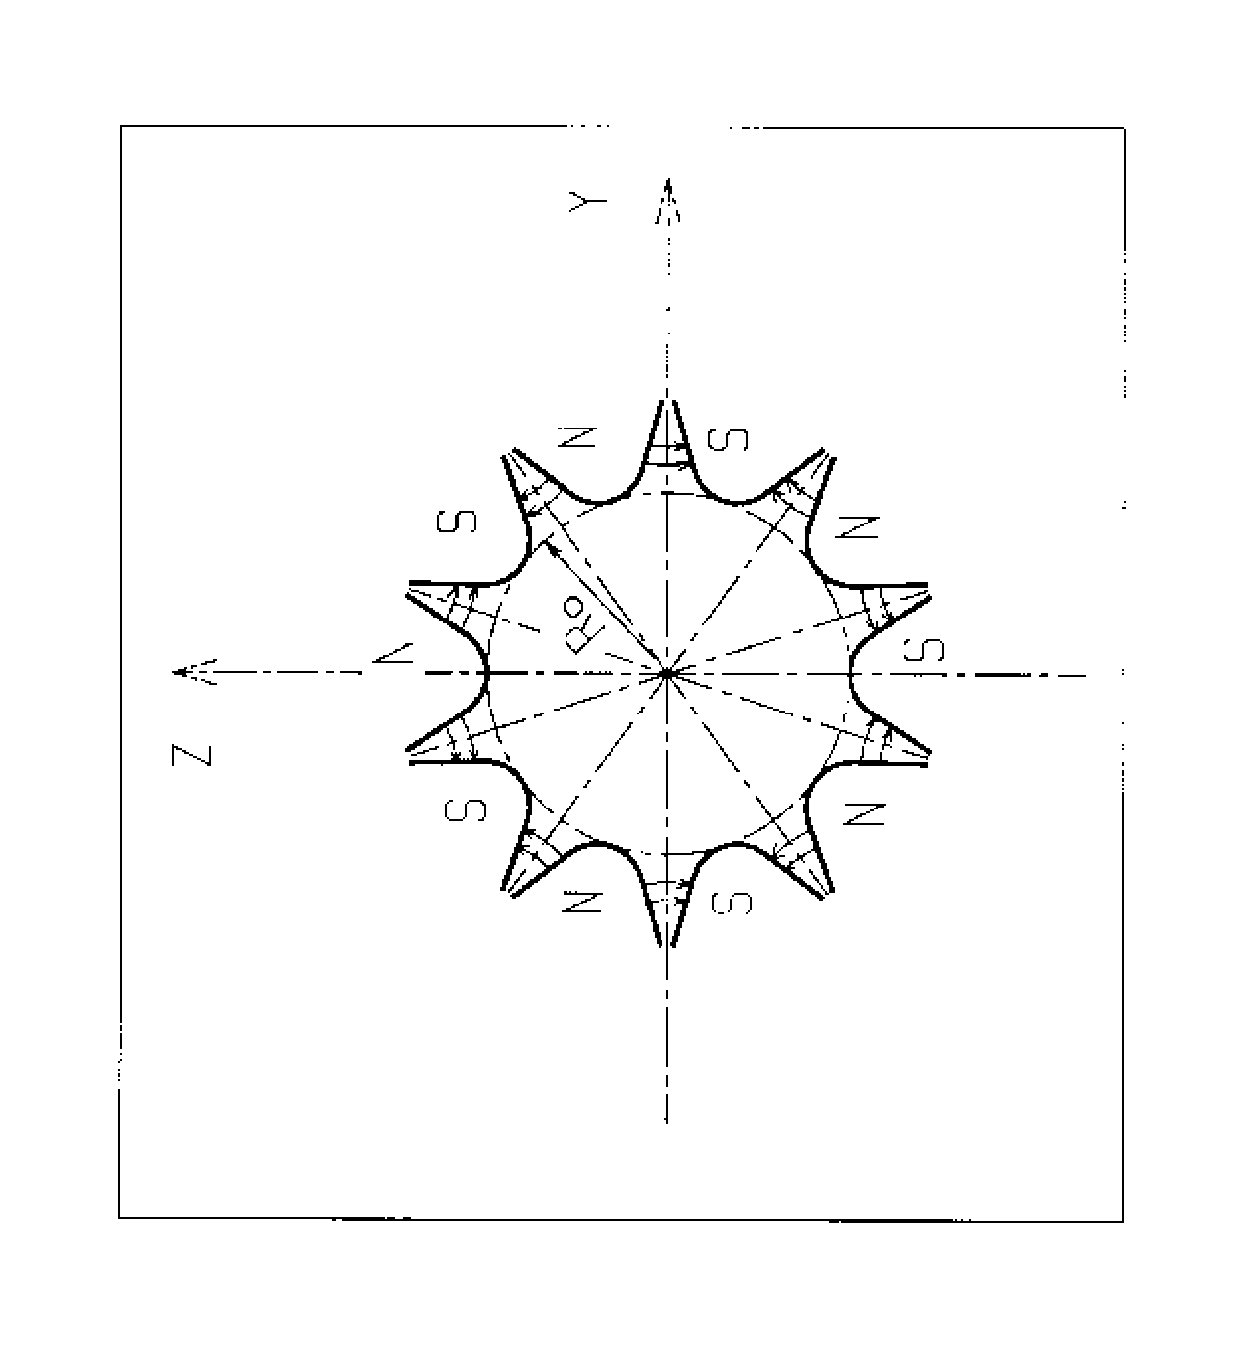
\includegraphics[width=12cm,angle=-90]{Fig18.ps}}
\caption{\label{fig18}Decapole magnet}
\end{figure}
\vfill








\newpage

\subsubsection*{DIPOLE~: \DIPOLETitl} \label{DIPOLE} \index{DIPOLE|textbf}
\medskip

\noindent\textsl{DIPOLE} provides a model of a dipole field, possibly with transverse indices. 
 The field along a particle trajectory is computed as the 
particle motion proceeds, straightforwardly from the dipole geometrical boundaries. 
Field simulation  in \textsl{DIPOLE}  is the same as used in \textsl{DIPOLE-M} and \textsl{AIMANT} 
for computing a field map~; the essential difference in \textsl{DIPOLE} is in its skipping that 
intermediate stage of field map generation found in \textsl{DIPOLE-M} and \textsl{AIMANT}. 

\bigskip

\noindent \textsl{DIPOLE}  has a version, \textsl{DIPOLES}, that allows overlapping of fringe fields 
in a configuration of neighboring magnets. 

\bigskip

\noindent The dimensioning of the magnet is defined by (Fig.~\ref{fig9}, p.~\pageref{fig9})

\bigskip

 \begin{tabular}{>{\sl}l!{~:}l}
	 AT &  total angular aperture \\
	 RM & mean radius used for the positioning of field boundaries\\
 \end{tabular}

\bigskip

\noindent The 2 or 3 effective field boundaries (EFB), from which  the dipole field  is drawn, are
defined from geometric boundaries, the shape and position of which are determined by the 
following parameters. 

\bigskip

\begin{tabular}{l!{~:}l}
	 \textsl{ACENT} 
	    & arbitrary inner angle, used for EFB's positioning  \\
	$\omega$ &  azimuth of an EFB with respect to  \textsl{ACENT}\\
	$\theta$ & angle of an EFB with respect to its azimuth (wedge angle)\\ 
	$R_1$, $R_2$  &  radius of curvature of an EFB\\
	$U_1$, $U_2$  &  extent of the linear part of an EFB. 
\end{tabular}

\bigskip


 \noindent The magnetic field is calculated in  polar
coordinates. At  any position $(R,\theta)$ along the  particle trajectory 
the value of the vertical component of the mid-plane field is calculated using

 \begin{equation}
	 B_Z(R,\theta) =  \mathcal{F}(R,\theta) \ast  B_0 \ast  
	      \left(1+N \ast  
	           \left( \dfrac{R-RM }{ RM}\right) 
	           + B \ast  \left(\dfrac{R-RM }{ RM} \right)^2 
	           + G \ast  \left(\dfrac{R-RM }{ RM} \right)^3 
	      \right) 
 	\label{eqBDipole}
 \end{equation}
 where  $ N$, $B $ and $ G $ are  respectively  the first, second and
third order field indices and $ \mathcal{F}(R,\theta)$ is the fringe field coefficient (it determines the ``flutter'' 
in periodic structures). 


\paragraph{Calculation of the Fringe Field Coefficient} 

\noindent With  each EFB a realistic extent of the fringe field, $\lambda$ 
(normally equal to the gap size), is associated and a fringe field coefficient
$ F $ is calculated. In the following $\lambda$ stands for either $ \lambda_ E $
(Entrance), $ \lambda_ S $ (Exit) or $ \lambda_ L $ (Lateral EFB).  


\bigskip

\noindent$ F $ is an exponential type fringe field (Fig.~\ref{fig11}, p.~\pageref{fig11}) 
given by~\cite{Biblio12}     %%% [12]

$$ F = \dfrac{1 }{ 1+ \exp P(s)} $$
%
 wherein $ s $ is the distance to the EFB and depends on $(R,\theta)$, and 

$$
    P(s) = C_0
       +C_1 \left(  \dfrac{s }{ \lambda} \right) 
       +C_2 \left( \dfrac{s }{ \lambda} \right)^2 
       + C_3 \left( \dfrac{s }{ \lambda} \right)^3 
       +C_4 \left( \dfrac{s }{ \lambda} \right)^4 
       + C_5 \left(\dfrac{s }{ \lambda} \right)^5 $$
       
\noindent It is also possible to simulate a shift of the \textsl{EFB}, by giving a non
zero value to the parameter \textsl{shift}.  $ s $ is then changed to $ s -$\textsl{shift} in the 
previous equation.   This allows small variations of the magnetic length.  
\bigskip

\noindent Let $ F_E $ (respectively $ F_S$, $F_L$)  be the fringe field
coefficient attached to the entrance (respectively exit, lateral) EFB. At any position on  a 
trajectory the resulting value of the fringe field coefficient (eq.~\ref{eqBDipole}) is

$$  \mathcal{F}(R,\theta) = F_E  \ast  F_S \ast   F_L $$
%
In particular, $F_L\equiv 1 $  if no lateral EFB is requested. 



\bigskip


\paragraph{Calculation of the  Mid-plane Field and Derivatives }

\noindent $ B_Z(R,\theta)$ in Eq.~\ref{eqBDipole} is 
computed at  the $n\times n$ nodes  ($n=3$ or $5$ in practice)  
of a ``flying'' interpolation grid in the median plane centered on the projection $m_0$ of 
the actual particle position $M_0$ as schemed 
in Fig.~\ref{FigGrid}. A polynomial interpolation is involved, of the form 

$$B_Z(R,\theta) = A_{00} + A_{10}\theta + A_{01}R + A_{20}\theta^2 + A_{11}\theta R + A_{02}R^2 $$

\noindent  that yields the requested   derivatives, using 
$$	A_{kl} = \dfrac{1 }{ k!l!}\,  \dfrac{\partial^{ k+l}B_Z }{ \partial \theta^k\partial r^l} $$

\noindent Note that, the source code contains the explicit analytical 
expressions of the coefficients $A_{kl}$ solutions of the normal 
equations, so that the operation {\it is not}   CPU time consuming. 

\begin{figure}[h]
 \begin{center}
\includegraphics*[bbllx=30,bblly=150,bburx=590,bbury=400,width=8.2cm,height=4.3cm]{grid.eps}
{\setlength{\captionwidth}{12cm}
  \hangcaption{ \small     \label{FigGrid}
Interpolation method.  
$m_0$ and $m_1$ are the projections in the median plane of particle positions $M_0$ and $M_1$  and separated 
by  $\delta s$, projection of the integration step. 
}}
  \end{center}
\end{figure}


\bigskip

\paragraph{Extrapolation Off Median Plane} 

\noindent From the vertical field $ \vec  B $ and  derivatives in the median plane, 
first a transformation from polar to Cartesian coordinates is 
performed, following eqs (\ref{eq2-4-8} or \ref{eq2-4-9}), then,  extrapolation off median plane is 
performed by means of Taylor expansions, following the procedure described in section~\ref{sec2.3.2}. 






\newpage

\subsubsection*{DIPOLE-M~: \DIPOLEMTitl} \label{DIPOLE-M} \index{DIPOLE-M|textbf}
\medskip

\noindent\textsl{DIPOLE-M} is a more recent, simpler and improved version of 
\textsl{AIMANT\index{AIMANT}}.  
\bigskip

\noindent The keyword \textsl{DIPOLE-M} provides an automatic generation of a dipole 
field map in polar coordinates. The extent of the map is defined by the 
following parameters, as shown in Figs.~\ref{fig9}A and~\ref{fig9}B.
\bigskip

 \begin{tabular}{>{\sl}l!{~:}l}
	 AT &  total angular aperture\\
	 RM & mean radius used for the positioning of field boundaries\\
	 RMIN, RMAX
	    &  minimum and maximum radii 
 \end{tabular}
\bigskip
 
\noindent The 2 or 3 effective field boundaries (EFB) inside the map are
defined from geometric boundaries, the shape and position of which are determined by the 
following parameters. 
\bigskip

\begin{tabular}{l!{~:}l}
	 \textsl{ACENT} 
	    & arbitrary inner angle, used for EFB's positioning  \\
	$\omega$ &  azimuth of an EFB with respect to  \textsl{ACENT}\\
	$\theta$ & angle of an EFB with respect to its azimuth (wedge angle)\\ 
	$R_1$, $R_2$  &  radius of curvature of an EFB\\
	$U_1$, $U_2$  &  extent of the linear part of an EFB. 
\end{tabular}
\bigskip


\noindent At  any node  of the map mesh, the value of the field is calculated as 

 \begin{equation}
	 B_Z(R,\theta)  =  \mathcal{F}(R,\theta)  \ast  B_0 \ast  
	      \left(1+N \ast  
	           \left( \dfrac{R-RM }{ RM}\right) 
	           + B \ast  \left(\dfrac{R-RM }{ RM} \right)^2 
	           + G \ast  \left(\dfrac{R-RM }{ RM} \right)^3 
	      \right) 
 	\label{eq3-3-1}
 \end{equation}
%
 where  $ N$, $B $ and $ G $ are  respectively  the first, second and
third order field indices and $ \mathcal{F}$ is the fringe field coefficient. 


\paragraph{Calculation of the Fringe Field Coefficient} 

\noindent With  each EFB a realistic extent of the fringe field, $\lambda $ 
(normally equal to the gap size), is associated and a fringe field coefficient
$ F $ is calculated. In the following $\lambda$ stands for either $ \lambda_ E $
(Entrance), $ \lambda_ S $ (Exit) or $ \lambda_ L $ (Lateral EFB).  
\bigskip

\noindent$ F $ is an exponential type fringe field (Fig.~\ref{fig11}) 
given by~\cite{Biblio12}     %%% [12]

$$ F = \dfrac{1 }{ 1+ \exp P(s)} $$
%
 where $ s $ is the distance to the EFB, and 

$$
    P(s) = C_0
       +C_1 \left(  \dfrac{s }{ \lambda} \right) 
       +C_2 \left( \dfrac{s }{ \lambda} \right)^2 
       + C_3 \left( \dfrac{s }{ \lambda} \right)^3 
       +C_4 \left( \dfrac{s }{ \lambda} \right)^4 
       + C_5 \left(\dfrac{s }{ \lambda} \right)^5 $$
       
\noindent It is also possible to simulate a shift of the \textsl{EFB}, by giving a non
zero value to the parameter \textsl{shift}.  $ s $ is then changed to $ s -$\textsl{shift} in the 
previous equation.   This allows small variations of the total magnetic length.  
\bigskip

\noindent Let $ F_E $ (respectively $ F_S$, $F_L$)  be the fringe field
coefficient attached to the entrance (respectively exit, lateral) EFB. At any node of the map 
mesh, the resulting value of the fringe field coefficient (eq.~\ref{eq3-3-1}) is

$$  \mathcal{F}(R,\theta) = F_E  \ast  F_S \ast   F_L $$
%
In particular, $F_L\equiv 1 $  if no lateral EFB is requested. 

\paragraph{The Mesh of the Field Map} 

\noindent The magnetic field is calculated at the nodes of a mesh with polar
coordinates, in the median plane.  The radial step is given by 

 \begin{align*}
	 \delta R & = \dfrac{\text{\textsl{RMAX}} - \text{\textsl{RMIN}} }{\text{\textsl{IRMAX}}-1} \\
	\intertext{and the angular step by} 
	 \delta \theta  & = \dfrac{AT }{\text{\textsl{IAMAX}}-1} 
 \end{align*}
 %
\noindent where \RMIN  and \RMAX\   are the lower and upper
radial limits of the field map, and $ AT $ is its total angular aperture (Fig.~\ref{fig9}B).  
 \textsl{IRMAX}  and \textsl{IAMAX} are 
the total number of nodes in the radial and angular directions. 

\paragraph{Simulating Field Defects and Shims }

\noindent Once the initial map is calculated, it is possible to modify it by
means of the parameter \textsl{NBS}, so as to simulate field defects or shims. 
\bigskip

\noindent\textbf{If $\mathbf{NBS = - 2}$,} the map is globally modified by a
perturbation proportional to $ R-R_0 $, 
where $ R_0 $ is an arbitrary radius, with an amplitude $ \Delta B_Z/B_0 $, so
that $ B_Z $ at the nodes of the mesh is replaced by 

$$ B_Z  \ast   \left(1+ \dfrac{\Delta B_Z }{ B_0}\, \dfrac{R-R_0 }{\text{\RMAX- \RMIN}} \right) $$

\noindent\textbf{If  $\mathbf{NBS =  - 1}$,} the perturbation is proportional to
$ \theta -\theta_ 0 $, and $ B_Z $ is replaced by 

$$ B_Z \ast  \left(1+ \dfrac{\Delta B_Z }{ B_0} \, \dfrac{\theta -\theta_ 0 }{ AT}\right) $$

\noindent\textbf{If  $\mathbf{NBS \geq 1}$,} then \textsl{NBS} shims are introduced at
positions $ \dfrac{ R_1+R_2 }{ 2}$, $\dfrac{\theta_ 1+\theta_ 2 }{ 2} $ 
(Fig.~\ref{fig13})~\cite{Biblio13}   %%%   [13] 

\noindent The initial field map is modified by shims with second order profiles given by 

$$ \theta  = \left(\gamma  + \dfrac{\alpha }{ \mu} \right) \,\beta\, \dfrac{X^2 }{\rho^ 2} $$
%
 where $ X $ is shown in  Fig.~\ref{fig11}, 
 $\rho = \dfrac{R_1+R_2 }{ 2} $ is the central radius, $\alpha$ and $\gamma$ are the angular 
 limits of the shim, $\beta$ and $\mu$ are parameters. 
 
\noindent At each shim, the value of $ B_Z $ at any node of the initial map is replaced by 

$$ B_Z \ast  \left(1+F\theta  \ast  FR \ast  \dfrac{\Delta B_Z }{ B_0} \right)
$$
%
 where $ F\theta =0 $ or $ FR=0 $ outside the shim, and $ F\theta =1$ and $ FR=1 $ inside.  
\bigskip

\paragraph{Extrapolation Off Median Plane} 

\noindent The vector field $ \vec  B $ and its derivatives in the median plane
are calculated by means of a second or fourth order polynomial 
interpolation, depending 
on the value of the parameter \textsl{IORDRE\index{IORDRE}} (\textsl{IORDRE}=2, 25 or 4, see 
section~\ref{sec2.4.2}). 
The transformation from polar to Cartesian coordinates is 
performed following eqs (\ref{eq2-4-8} or \ref{eq2-4-9}). Extrapolation off median plane is then 
performed by means of Taylor expansions, following the procedure described 
in section~\ref{sec2.3.2}. 









\newpage

\subsubsection*{DIPOLES~: \DIPOLESTitl~\cite{reportNIMFFAG,reportICFAFFAG}} \label{DIPOLES} \index{DIPOLES|textbf}
\medskip

\noindent \textsl{DIPOLES} works much like \textsl{DIPOLE\index{DIPOLE}} 
as to the field modelling, yet with the particularity that it allows positioning up to 5 such 
dipoles within the angular sector with full aperture $AT$ thus allowing 
accounting for overlapping fringe fields.\index{fringe fields overlapping} 
This is done in the following 
way\footnote{\textsl{FFAG} can be referred to as another instance of a procedure based on such method.}. 

\bigskip

\noindent  The dimensioning of the magnet is defined by

\bigskip

 \begin{tabular}{>{\sl}l!{~:}l}
	 AT &  total angular aperture \\
	 RM & mean radius used for the positioning of field boundaries\\
 \end{tabular}

\bigskip

\noindent For each one of the $N=1$ to $5$ dipoles of the  $N$-tuple, 
the 2 effective field boundaries (entrance and exit EFBs) from which  the dipole field  
 (eqs.~\ref{EqFieldDipolesi},~\ref{EqFieldDipolesii})  is drawn are
defined from geometrical  boundaries, the shape and position of which are determined by the 
following parameters (in the same manner as in \textsl{DIPOLE}, \textsl{DIPOLE-M})
 (see Fig.~\ref{fig9}-A, p.~\pageref{fig9}, and Fig.~\ref{figDFD}) 

\bigskip

\begin{tabular}{l!{~:}l}
	$ACN_i$  & arbitrary inner angle, used for EFB's positioning  \\
	$\omega$ &  azimuth of an EFB with respect to  \textsl{ACN}\\
	$\theta$ & angle of an EFB with respect to its azimuth (wedge angle)\\ 
	$R_1$, $R_2$  &  radius of curvature of an EFB\\
	$U_1$, $U_2$  &  extent of the linear part of an EFB  \\
\end{tabular}

\bigskip

\paragraph{Calculation of the Field From a Single Dipole} 

 \noindent The magnetic field is calculated in  polar
coordinates.  At all $(R,\theta)$ in the median plane ($Z=0$), the 
magnetic field  due  a single one (index $i$) of the  dipoles  of a $N$-tuple   magnet can 
take either form, upon option, 

\begin{eqnarray}
(i) & ~ ~ \Bz_i(R,\theta) =  \Bz_{0,i} \, \mathcal{F}_i(R,\theta) \, 
\left( 1 +  b_{1_i} (R-RM_{i})/RM_{i} + b_{2_i} (R-RM_{i})^2/RM_{i}^2 +... \right)  \label{EqFieldDipolesi} \\
%\left(   b_{0_i}  +  b_{1_i} (R-RM_{i})/RM_{i} + b_{2_i} (R-RM_{i})^2/RM_{i}^2 +... \right)
 (ii) & ~   B_Z(R,\theta) =  \Bz_{0,i} \, + \, \sum_{i=1}^N  \mathcal{F}_i(R,\theta) \, 
\left( b_{1_i} (R-RM_{i}) + b_{2_i} (R-RM_{i})^2 +... \right)
\label{EqFieldDipolesii}
\end{eqnarray}
%
\noindent wherein $\Bz_{0,i}$  is a reference field, at reference radius  $RM_{i}$, 
 and $ \mathcal{F}(R,\theta)$ is the fringe field coefficient, see below. 
This field model is proper to simulate for instance chicane dipoles,  cyclotron 
\index{cyclotron} or FFAG\index{FFAG magnet, radial} \index{FFAG}  magnets, etc. 


\begin{figure}[h]
 \begin{center}
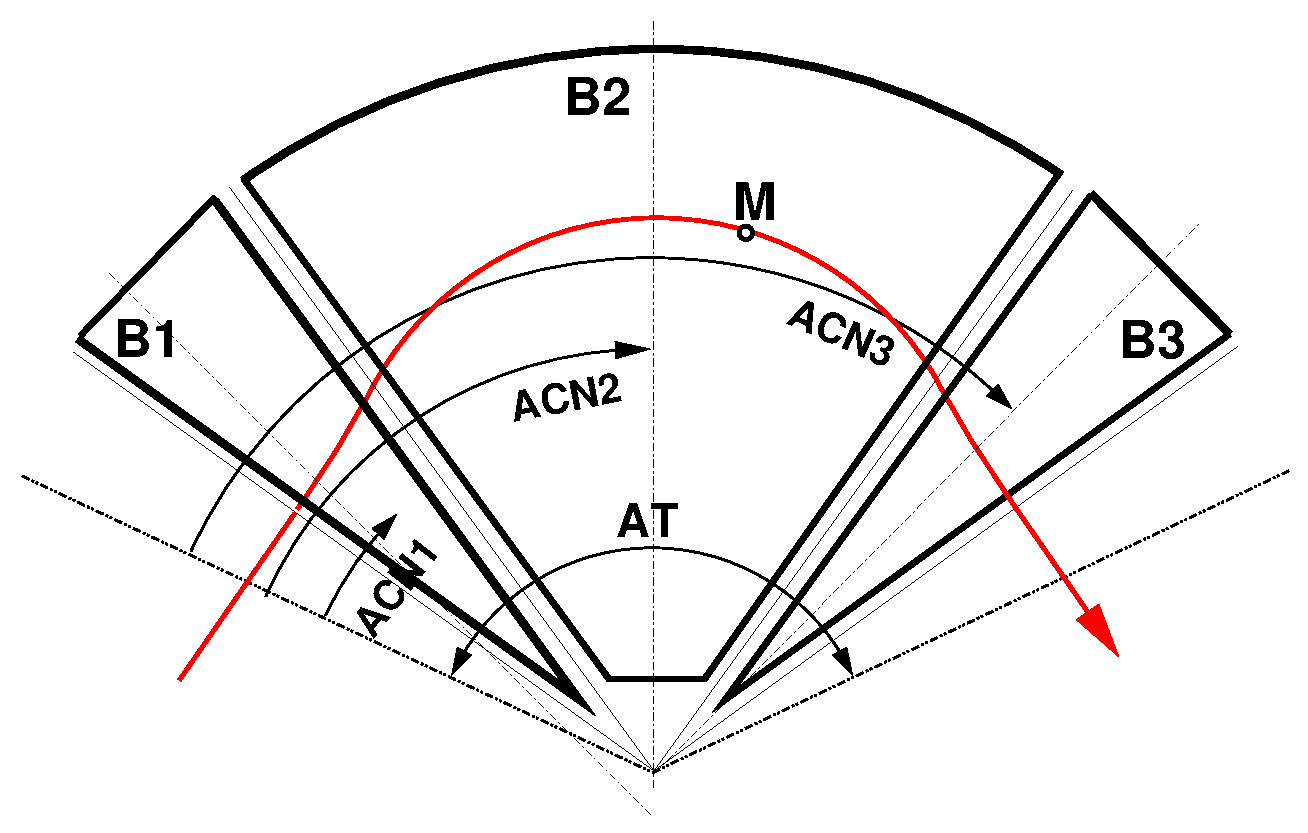
\includegraphics[width=8.5cm]{ffagTriplet.eps}  
 \caption{ \label{figDFD}
Definition of a dipole triplet using  the \textsl{DIPOLES} or  \textsl{FFAG}  procedures. 
}
  \end{center}
\end{figure}





\paragraph{Calculation of the Fringe Field Coefficient} 

\noindent In a dipole, a realistic extent of the fringe field, $g $, 
is associated with  each EFB, and a fringe field coefficient $ F $ is calculated. 


\bigskip

\noindent$ F $ is an exponential type fringe field (Fig.~\ref{fig11}, page~\pageref{fig11}) 
given by~\cite{Biblio12}     %%% [12]

$$ F = \dfrac{1 }{ 1+ \exp P(d)} $$
%
 wherein $ d $ is the distance to the EFB and depends on $(R,\theta)$, and 

$$
    P(d) = C_0
       +C_1 \left(  \dfrac{d }{ g } \right) 
       +C_2 \left( \dfrac{d }{ g } \right)^2 
       + C_3 \left( \dfrac{d }{ g } \right)^3 
       +C_4 \left( \dfrac{d }{ g } \right)^4 
       + C_5 \left(\dfrac{d }{ g } \right)^5 $$

\noindent In addition,   $g$ is made dependent  of $R$ 
(a way to simulate the effect of variable gap size on fringe field extent), 
under the form 

$$ g(R) = g_0 \, (RM/R)^{\kappa}  $$

\noindent  This dependence is accounted for rigorously if the interpolation method (see below) is 
used, or else to  order zero (derivatives of $g(R)$ are not considered) if the analytic method 
(below) is used. 

\smallskip

\noindent Let $ F_E $ (respectively $ F_S$)  be the fringe field
coefficient attached to the entrance (respectively exit) EFB~; at any position on  a 
trajectory the resulting value of the fringe field coefficient is taken to be 

\begin{equation}
\label{EqFFdips}
  \mathcal{F}_i(R,\theta) = F_E  \ast  F_S 
\end{equation}



\paragraph{Calculation of the  Field Resulting From all $N$ Dipoles \label{FFatAP}}

 
\noindent Now, accounting for   $N$ neighboring dipoles in an $N$-tuple,  the mid-plane field  and field derivatives  
are  obtained by addition of  the  contributions of the $N$ dipoles taken separately, namely

\begin{eqnarray}
\label{EqSumB}
\Bz(R,\theta) &=&  \sum_{i=1,N} \Bz_i(R,\theta)   \\
\dfrac{\partial^{ k+l}\vec \Bz(R,\theta) }{ \partial \theta^k\partial r^l} &=&  \sum_{i=1,N} 
\dfrac{\partial^{ k+l}\vec \Bz_i(R,\theta) }{ \partial \theta^k\partial r^l} 
\end{eqnarray}

\noindent  Note that, in doing so it is not meant that field superposition  does apply 
in reality, it is just meant to provide the possibility 
of obtaining a realistic  field shape, that would for instance closely match (using appropriate $C_0-C_5$ sets 
of coefficients) 3-D  field simulations obtained from magnet design codes. 


\bigskip




\paragraph{Calculation of the  Mid-plane Field Derivatives}

\noindent Two  methods have been implemented to calculate the field derivatives in the median 
plane (Eq.~\ref{EqSumB}), based on 
 either analytical expressions derived from the magnet geometrical description,  or  classical numerical interpolation. 
 
\noindent The first method has the merit of insuring best symplecticity in principle and fastest tracking. 
The interest of the second method is in its  facilitating possible  changes in 
  the mid-plane magnetic field model $\Bz(R,\theta)$, for instance if simulations of shims, defects, 
or special $R, \theta$  field dependence need to be introduced. 



\bigskip

\noindent {\it Analytical method~\cite{theseLemuet}~: }\label{AnalMeth}

\bigskip

\noindent The  starting ingredients are, on the one hand distances to the EFBs,  

$$d(R,\theta)=\sqrt{(x(R,\theta)-x_{0}(R,\theta))^2+(y(R,\theta)-y_{0}(R,\theta))^2}$$

\noindent to be computed for the two cases $d_{\textrm{Entrance}}$, $d_{\textrm{Exit}}$, and 
on the other hand the expressions of the coordinates of particle position $M$ and its projection $P$ on 
the EFB in terms of the magnet geometrical parameters, namely 

\begin{eqnarray}
x(R,\theta)&=&\cos (ACN-\theta)-RM   \nonumber \\[-1ex]
y(R,\theta)&=&R\sin (ACN-\theta)   \nonumber \\[-1ex]
x_P(R,\theta)&=&\sin(u)\:  (y(R,\theta) - y_b)/2 + x_b\:  \sin^2(u) + x(R,\theta)\:  \cos^2(u)   \nonumber \\[-1ex]
y_P(R,\theta)&=&\sin(u)\: (x(R,\theta) - x_b)/2 + y_b\:  \cos^2(u) + y(R,\theta) \: \sin^2(u)   \nonumber 
\end{eqnarray}

\noindent with $x_b,~y_b,~u$ parameters drawn from the  magnet geometry (sector angle, wedge angle, face curvatures, etc.). 

\noindent These ingredients allow calculating  the derivatives 
$\dfrac{\partial^{ u+v}x(R,\theta)}{ \partial \theta^u\partial r^v}\:,$ 
$\:\: \dfrac{\partial^{ u+v}y(R,\theta)}{ \partial \theta^u\partial r^v}\:,$ 
$\:\:\dfrac{\partial^{ u+v}x_0(R,\theta)}{ \partial \theta^u\partial r^v}\:,$ 
$\:\:\dfrac{\partial^{ u+v}y_0(R,\theta)}{ \partial \theta^u\partial r^v}\:,$ 
which, in turn,  intervene in the derivatives of the compound functions 
$\dfrac{\partial^{ u+v}F(R,\theta)}{ \partial \theta^u\partial r^v}\:,$ 
$\:\:\dfrac{\partial^{ u+v}p(R,\theta)}{ \partial \theta^u\partial r^v}\:,$ 
$\:\:\dfrac{\partial^{ u+v}d(R,\theta)}{ \partial \theta^u\partial r^v}$. 


\bigskip

\noindent { \it Interpolation method~:  \label{CalcMidPlaneFieldInterpol}}\label{InterpMeth}

\bigskip

\noindent The expression $\Bz(R,\theta)$ in Eq.~\ref{EqSumB} is, in this case, 
computed at  the $n\times n$ nodes  ($n=3$ or $5$ in practice)  
of a ``flying'' interpolation grid in the median plane centered on the projection $m_0$ of 
the actual particle position $M_0$ as schemed 
in Fig.~\ref{FigGrid2}. A polynomial interpolation is involved, of the form 

$$\Bz(R,\theta) = A_{00} + A_{10}\theta + A_{01}R + A_{20}\theta^2 + A_{11}\theta R + A_{02} R^2 $$

\noindent  that yields the requested   derivatives, using 
$$	A_{kl} = \dfrac{1 }{ k!l!}\,  \dfrac{\partial^{ k+l}B }{ \partial \theta^k\partial r^l} $$

\noindent Note that, the source code contains the explicit analytical 
expressions of the coefficients $A_{kl}$ solutions of the normal 
equations, so that the operation {\it is not}   CPU time consuming. 

\begin{figure}[h]
 \begin{center}
\includegraphics*[bbllx=30,bblly=150,bburx=590,bbury=400,width=8.2cm,height=4.3cm]{grid.eps}
{\setlength{\captionwidth}{12cm}
  \hangcaption{ \small     \label{FigGrid2}
Interpolation method.  
$m_0$ and $m_1$ are the projections in the median plane of particle positions $M_0$ and $M_1$  and separated 
by $\delta s$, projection of the integration step. 
}}
  \end{center}
\end{figure}


\bigskip

\paragraph{Extrapolation Off Median Plane} 

\noindent From the vertical field $ \vec  B $ and  derivatives in the median plane, 
first a transformation from polar to Cartesian coordinates is 
performed, following eqs (\ref{eq2-4-8} or \ref{eq2-4-9}), then,  extrapolation off median plane is 
performed by means of Taylor expansions, following the procedure described in section~\ref{sec2.3.2}. 




\bigskip

\paragraph{Sharp Edge} 

\noindent Sharp edge field fall-off at a field boundary  can only be simulated if the following conditions are fulfilled~: 

- entrance (resp. exit)  field boundary  coincides with entrance (resp. exit) 
dipole limit (it means in particular, see Fig.~\ref{fig9},  
$\omega^+= ACENT$ (resp. $\omega^- = -(AT-ACENT)$), 
together with $\theta=0$ at entrance (resp. exit) EFBs), 

- analytical method for calculation of the  mid-plane field derivatives is used. 








\newpage

\subsubsection*{DODECAPO~: \DODECAPOTitl\  (Fig.\protect~\ref{fig19})} \label{DODECAPO}  \index{DODECAPO|textbf}
\medskip


 The meaning of parameters for \textsl{DODECAPO}  is the same as for \textsl{QUADRUPO}. 
%\bigskip

\noindent In fringe field regions the magnetic field $ \vec  B(X,Y,Z) $ and
its derivatives up to fourth order are derived from the scalar potential approximated to 
the 6th order in $ Y $ and $ Z $ 

\begin{align*}
	V(X,Y,Z) &   = G(X) \left(Y^4- \dfrac{10 }{ 3} Y^2Z^2+Z^4 \right) YZ  \\
	\text{with } ~ G_0 &   =  \dfrac{ B_0 }{ R^5_0} 
\end{align*}

\noindent The  modelling of the fringe field form factor  $G(X)$
 is described under \textsl{QUADRUPO}, p.~\pageref{QUADRUPO}. 

\bigskip

\noindent Outside fringe field regions, or everywhere in sharp edge dodecapole
($ \lambda_ E=\lambda_ S=0$) , $ \vec  B(X,Y,Z) $ in the magnet is given by 

\begin{align*}
	B_X &   =   0 \\
	B_Y &   =    G_0(5Y^4-10Y^2Z^2+Z^4)Z \\
	B_Z &   = G_0(Y^4-10Y^2Z^2+5Z^4)Y  
\end{align*}
\vfill

%%%%%%%%%%%%%%figure%%%%%%%%%%%%%%
\begin{figure}[H]
%\vspace{12 truecm}
%%%Figure 19
\centerline{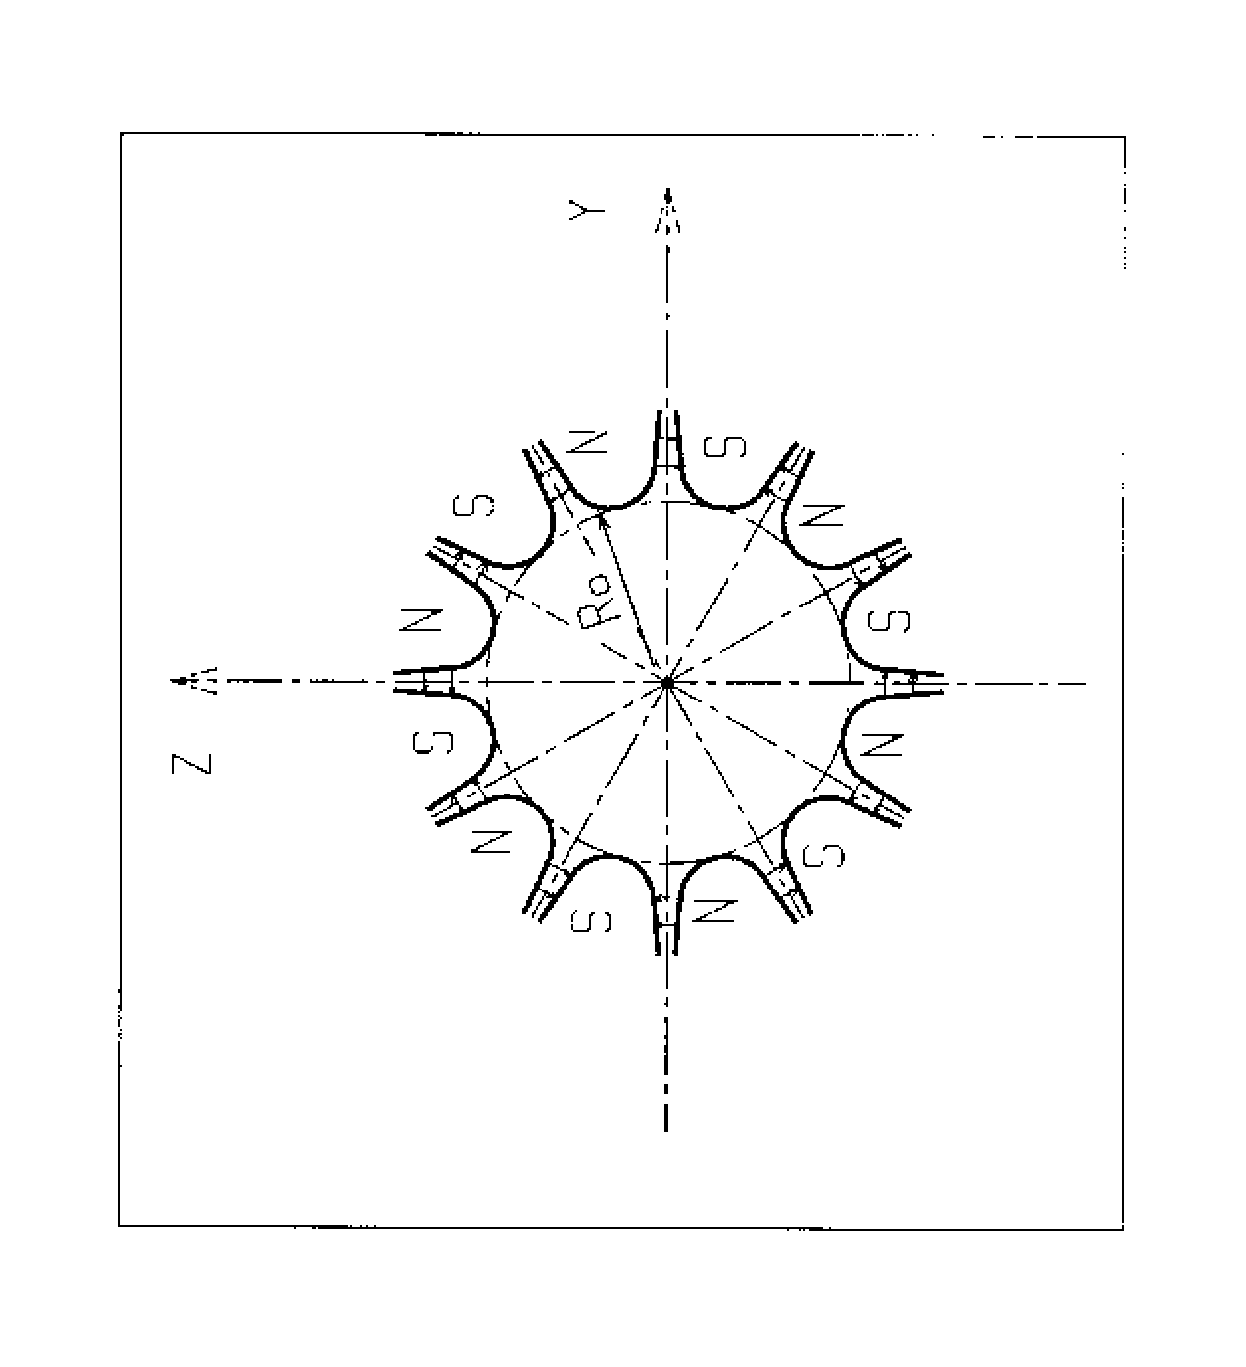
\includegraphics[width=12cm,angle=-90]{Fig19.ps}}
\caption{\label{fig19}Dodecapole magnet}
\end{figure}
\vfill

\newpage
\subsubsection*{DRIFT or ESL~: \DRIFTTitl}\label{ESL}\label{DRIFT}\index{DRIFT|textbf}\index{ESL|textbf}
\medskip

\textsl{DRIFT} or \textsl{ESL} allow introduction of a drift space with length $ \XL $ with 
positive or negative sign, anywhere in a structure.  The associated equations 
of motion are (Fig.~\ref{fig23})   

\begin{align*}
	Y_2 &   =    Y_1+\XL \ast \text{tg} T  \\ 
	Z_2 &   =   Z_1 + \dfrac{\XL}{\cos  T}\,  \text{tg} P  \\
	SAR_2 &   =  SAR_1+ \dfrac{\XL }{\cos  T  \ast \cos  P}  
\end{align*}
\vfill

%%%%%%%%%%%%%%figure%%%%%%%%%%%%%%
\begin{figure}[H]
%\vspace{15 truecm}
%%%Figure 23
\centerline{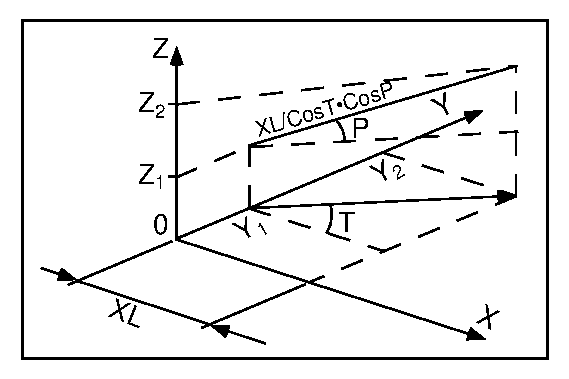
\includegraphics[width=15cm]{Fig23.ps}}
\caption{\label{fig23}Transfer of particles in a drift space.}
\end{figure}
\vfill

\newpage
\subsubsection*{EBMULT~: \EBMULTTitl}\label{EBMULT} \index{EBMULT|textbf}
\medskip

\noindent\textsl{EBMULT} simulates an electro-magnetic multipole, by addition of
electric $ (\vec  E) $ and magnetic $ (\vec  B) $ multipole components (dipole to 20-pole). 
$\vec  E $ and its derivatives 
$ \dfrac{\partial^{ i+j+k} \vec  E }{ \partial X^i\partial Y^j\partial Z^k} $ 
($i+j+k \le 4$) are derived 
from the general expression of the multipole scalar potential (eq.~\ref{eq2-3-5}), followed by a 
$ \dfrac{\pi }{2n} $ rotation  ($n= 1, 2, 3, ...$)  (see also \textsl{ELMULT\index{ELMULT}}). $ \vec  B $ and its
derivatives are derived from the same general potential, as described in section~\ref{sec2.3.5} 
(see also \textsl{MULTIPOL\index{MULTIPOL}}). 

\bigskip

\noindent The entrance and exit fringe fields of the $ \vec  E $ and $ \vec  B$ components are treated 
separately, in the same way as described under \textsl{ELMULT\index{ELMULT}} 
 and \textsl{MULTIPOL\index{MULTIPOL}},
for each one of these two fields. Wedge angle correction is applied in sharp edge field model if $ \vec  B1$ is non zero, as in \textsl{MULTIPOL}. Any of the $ \vec  E $ or $ \vec  B $ multipole field
component can be $X$-rotated independently of the others. 

\bigskip

\noindent Use \textsl{PARTICUL\index{PARTICUL}} prior to \textsl{EBMULT}, for the 
 definition of  particle mass and charge.
\vfill

%%%%%%%%%%%%%%figure%%%%%%%%%%%%%%
\begin{figure}[H]
%\vspace{15 truecm}
%%%Figure 20
\centerline{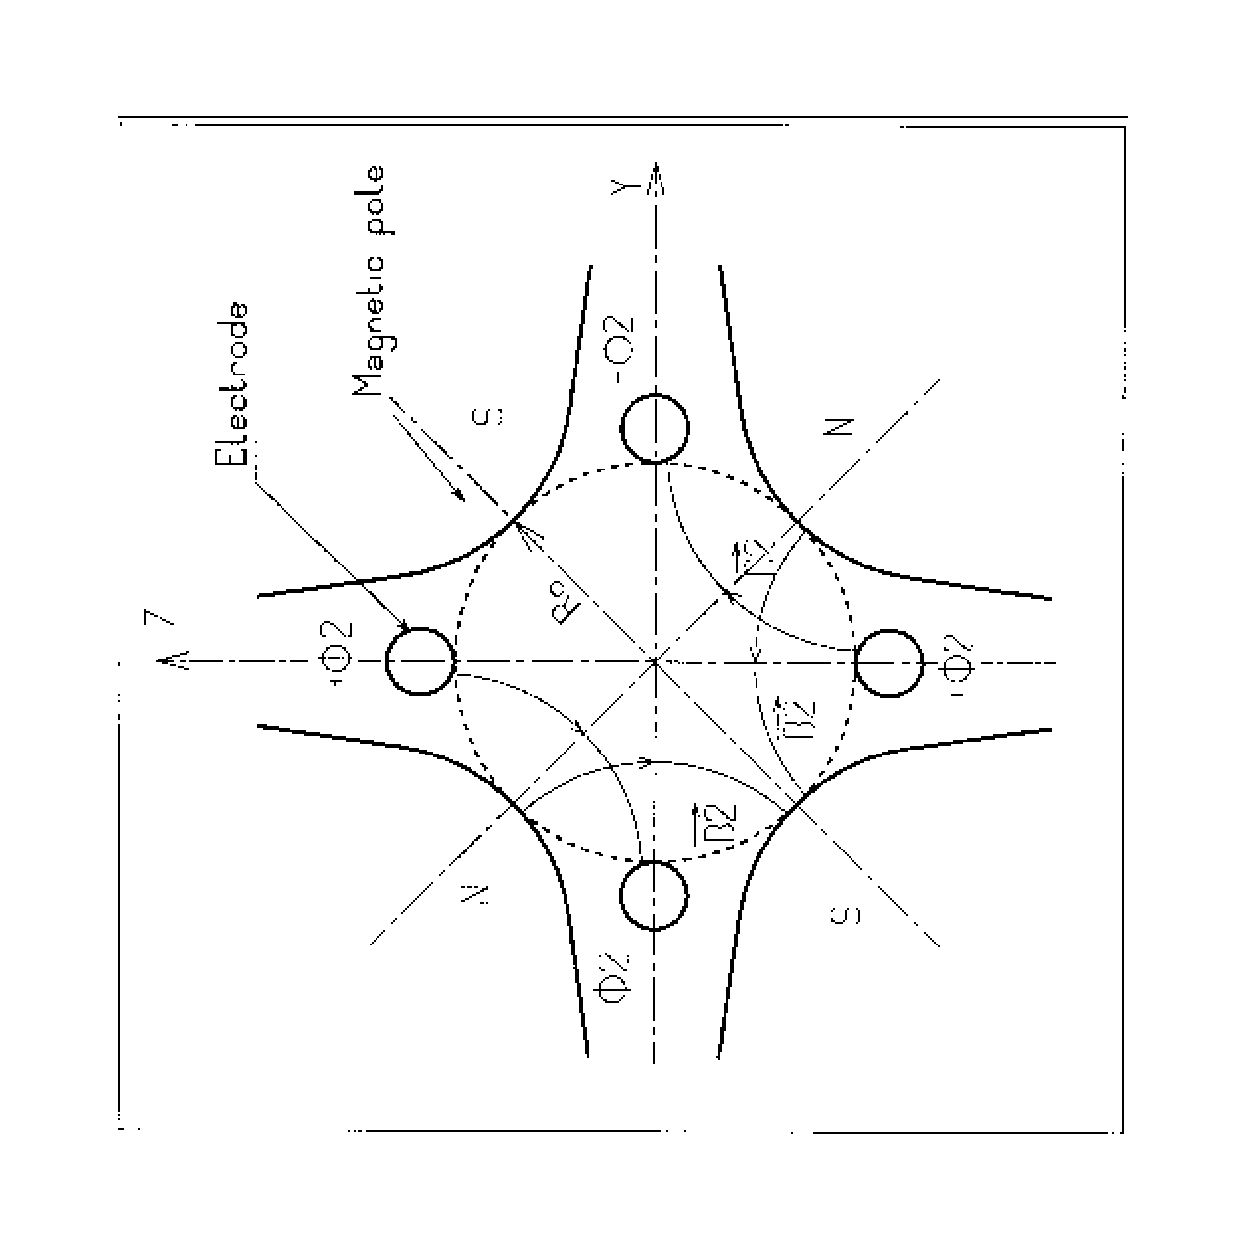
\includegraphics[height=11cm,angle=-90]{Fig20.ps}}
\hangcaption[Fig20]{\label{fig20}An example of $ \vec  E$, $\vec  B $ multipole~: 
           the achromatic quadrupole  \\  
          (known for its allowing null second order chromatic aberrations~\protect\cite{Biblio14}).}
\end{figure}

\newpage

\subsubsection*{EL2TUB~: \ELTwoTUBTitl} \label{EL2TUB} \index{EL2TUB|textbf}
\medskip

The lens is cylindrically symmetric about the $ X$-axis. 

\noindent The length and potential of the first (resp. second) electrode 
are $ X1 $ and $ V1 $ ($ X2 $ and $ V2$).   The distance between the two 
electrodes is $ D$,   and their inner radius is $ R_0 $ (Fig.~\ref{fig22}).   
The model for the electrostatic potential along the axis is~\cite{Biblio16}     %% [16]

 \begin{alignat*}{2}
	 V(X) &   = \dfrac{ V_2-V_1}{2} \: \text{th}\,
	            \dfrac{\omega x }{ R_0} 
	             \left[+ \dfrac{V_1+V_2 }{ 2} \right] 
	      & \qquad \text{if }  D & =0\\
	V(X) &  =  \dfrac{ V_2-V_1 }{ 2}\: \dfrac{1}{ 2\omega D/R_0} \: \ell n\,
	           \dfrac{\text{ch}\, \omega\,    \dfrac{x+D }{ R_0} }%
	           {\text{ch} \,\omega \,\dfrac{x-D }{ R_0}}
	           \left[+ \dfrac{V_1+V_2 }{ 2} \right]   
	            & \qquad \text{if }  D &  \not= 0 
 \end{alignat*}
%
($ x $ = distance from half-way between the electrodes~;
$\omega$  =  1.318~; th =  hyperbolic tangent~; ch  =  hyperbolic cosine)
from which the field $ \vec  E(X,Y,Z) $ and its derivatives are derived following the 
procedure described in section~\ref{sec2.5.2}  (note that they don't 
depend on the constant term $ \left[\dfrac{V_1+V_2 }{ 2} \right] $ which
disappears when differentiating). 

\medskip

\noindent Use \textsl{PARTICUL\index{PARTICUL}} prior to \textsl{EL2TUB}, for the
 definition of  particle mass and charge.

\vfill

%%%%%%%%%%%%%%figure%%%%%%%%%%%%%%
\begin{figure}[H]
%\vspace{13 truecm}
%%%Figure 22
\centerline{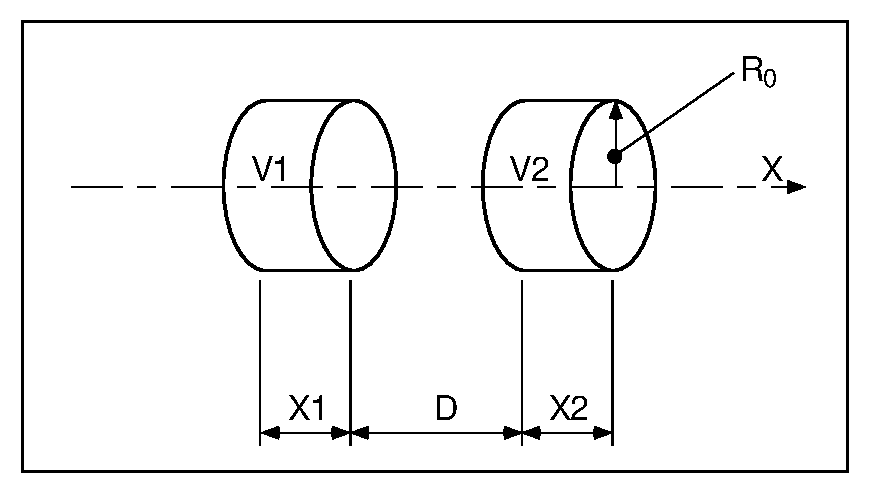
\includegraphics[width=14cm]{Fig22.ps}}
\caption{\CapELtwoTUB \label{fig22}}
\end{figure}

\vfill

\newpage

\subsubsection*{ELMIR~: \ELMIRTitl }\label{ELMIR}\index{ELMIR|textbf}
\medskip

The device works as  mirror or lens, horizontal or vertical. 
It is made of $N$ 2-plate electrodes and has mid-plane symmetry.  
\bigskip

\noindent Electrode lengths are  $ L\!1 $, $ L\!2 $, ...,   $ L\!N$. $D$ is the  mirror/lens gap. 
The model for the $Y$-independent electrostatic potential is (after Ref.~\cite[p.412]{Karets}) 
$$ V(X,Z) = 
   \sum_{i=2}^{N} \dfrac{V{i}-V{i\!-\!\textrm{\footnotesize 1}} }{ \pi} 
     \arctan\dfrac{\sinh(\pi ( X - X{i\!-\!\textrm{\footnotesize 1}})/D)}{\cos(\pi Z/D)}   
$$
where $V\!i$ are the potential at the $N$ electrodes (and normally $V\!1=0$ refers to 
the incident beam energy),   $X\!i$ are the  locations of the zero-length slits, $ X $ is the distance 
from the origin taken at the first slit (located at $X\!1 \equiv 0$ between the first and 
second electrodes).  
 From $V(X,Z) $ the field $ \vec  E(X,Y,Z) $ and derivatives are deduced following the procedure 
described in section~\ref{sec2.3.5}~(page~\pageref{sec2.3.5}).  

\medskip

\noindent The total X-extent of the mirror/lens is $L = \sum_{i=1}^N L\!i$.

\medskip

\noindent In the mirror mode (option  $\MT=11$ for vertical mid-plane  or $\MT=12$ 
for horizontal mid-plane) stepwise integration starts 
at $X=-L\!1$ (entrance of the first electrode) and terminates either when back to   $X=-L\!1$  
or when  reaching $ X=L-L\!1$ (end of the $N-th$ electrode). 
In the latter case particles  are stopped  with their index
 $I\!E\!X$ set to $-8$ (see section~\ref{sec4.6.6} on page~\pageref{sec4.6.6}). 
Normally $X\!1$ should   exceed  $3D$ (enough that $V(X<X\!1)$   have negligible effect in terms of trajectory behavior).  

\medskip

\noindent In the lens mode (option flag $\MT=21$ for vertical mid-plane  or $\MT=22$
for horizontal mid-plane) stepwise integration starts
at $X=-L\!1$ (entrance of the first electrode) and terminates either when reaching $ X=L-L\!1$ (end of the $N-th$ electrode) 
or when the particle deflection exceeds $\pi/2$. In the latter case the particle is stopped  with their index
 $I\!E\!X$ set to $-3$. 
 
\medskip

\noindent Use \textsl{PARTICUL\index{PARTICUL}} prior to \textsl{ELMIR}, for the
 definition of particle mass and charge.

\bigskip
\vfill

%%%%%%%%%%%%%%figure%%%%%%%%%%%%%%
\begin{figure}[H]
\centerline{\fbox{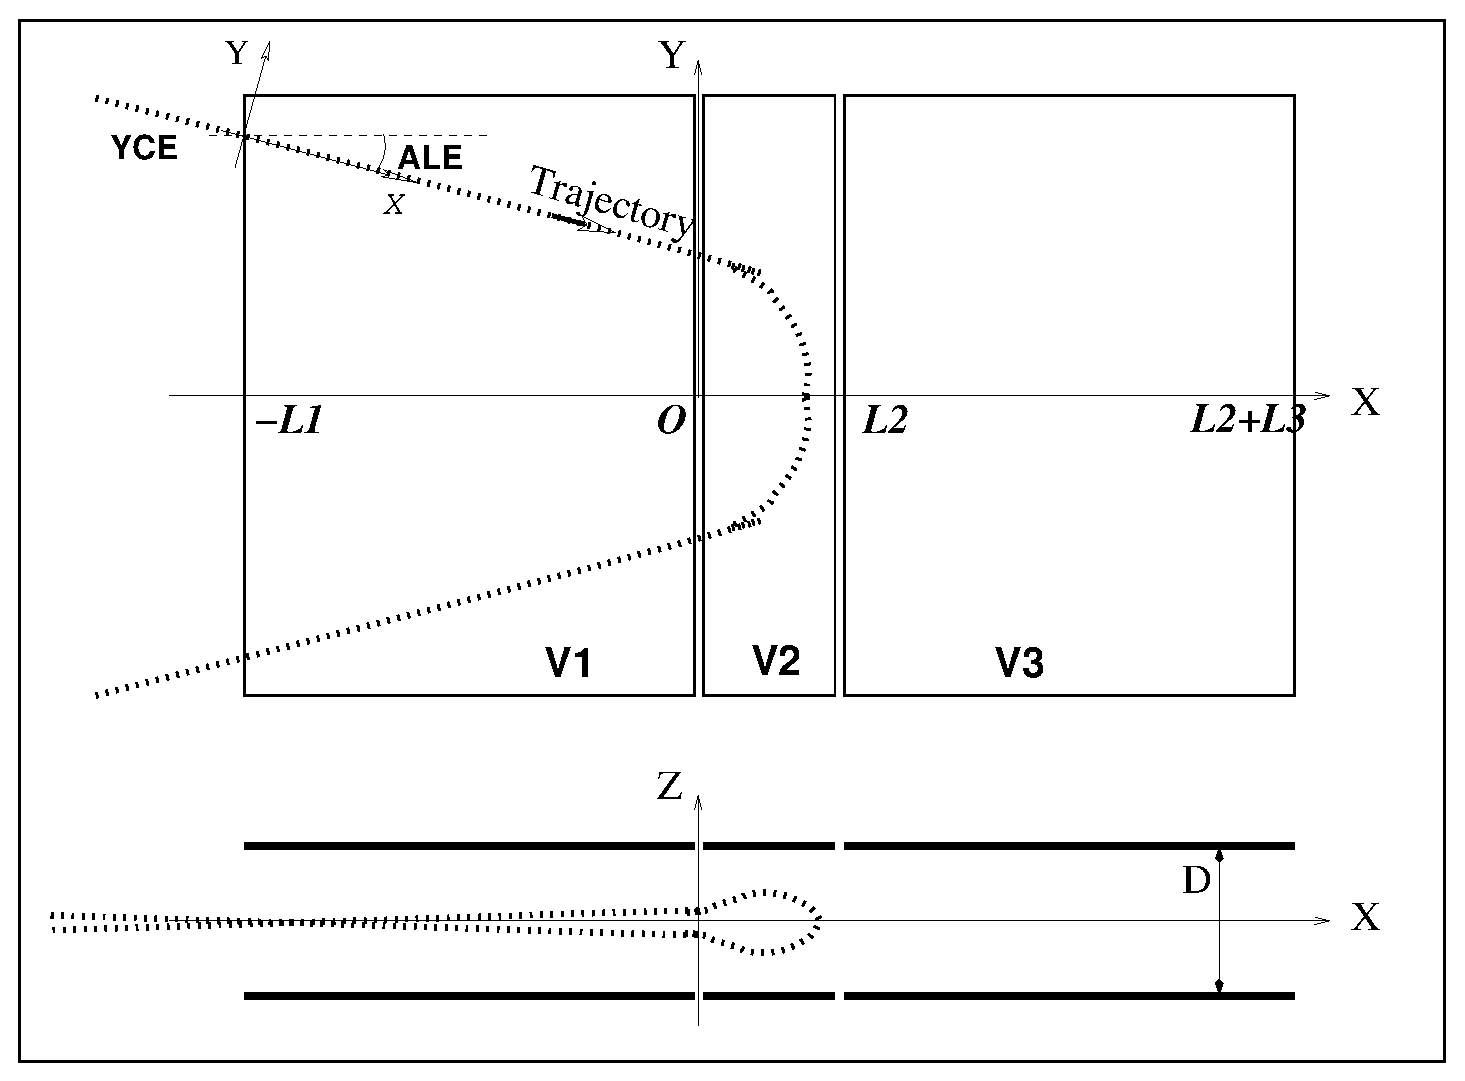
\includegraphics[height=8cm]{FigELMIR.eps}}}
\hangcaption{\label{figELMIR} \CapELMIR}
\end{figure}

\vfill

\newpage

\subsubsection*{ELMIRC~: \ELMIRCTitl~\cite{Karets}}\label{ELMIRC}\index{ELMIRC|textbf}
\medskip

The device works as  mirror or lens, horizontal or vertical. 
It is made of $N$ 2-plate electrodes and has mid-plane 
symmetry\footnote{NOTE~: in the present version of the code, the sole horizontal mirror mode 
 is operational, and $N$ is limited to 3.}. 

\medskip

\noindent Electrode  slits are circular, concentric with  radii  $ R1 $, $ R2 $, ...,   
$ R{\textrm{\footnotesize N-1}}$, 
$D$ is the  mirror/lens gap. The model for the mid-plane ($Z=0$) radial electrostatic potential  
is (after Ref.~\cite[p.443]{Karets})
$$ V(r) = 
   \sum_{i=2}^{N} \dfrac{V{i}-V{i\!-\!\textrm{\footnotesize 1}} }{ \pi} 
     \arctan \left( \sinh \dfrac{ \pi ( r - R{i\!-\!\textrm{\footnotesize 1}})}{D} \right)  
%    \dfrac{V-V\!A }{ \pi} \arctan \sinh \dfrac{\pi (r -R1)}{D} + 
%  \dfrac{V\!B - V }{ \pi} \arctan \sinh \dfrac{\pi (r -R2)}{D} 
$$
where $V\!i$ are the potential at the $N$ electrodes (and normally $V\!1=0$ refers to
the incident beam energy). $r$ is the current radius. 

\medskip

\noindent  The mid-plane field $ \vec  E(r) $ and its $r$-derivatives are first derived by differentiation, then 
$ \vec  E(r,Z) $ and  derivatives are obtained from Taylor expansions and Maxwell relations. 
Eventually a transformation to the rotating frame provides $\vec  E(X,Y,Z)$ 
 and  derivatives as involved in eq.~\ref{eq2-2-12}. 


\noindent Stepwise integration starts at entrance (defined by $R\!E, T\!E$) of the first electrode 
and terminates when rotation of the reference  rotating frame  $(RM,X,Y)$ has reached the value AT. 
Normally, $R1-R\!E$ and $R1-R\!S$ should both  exceed  $3D$ (so 
 that potential tails  have negligible effect in terms of trajectory behavior).  

\medskip

\noindent Positioning of the element is performed by means of \textsl{KPOS} (see section~\ref{sec4.6.2}). 

\medskip

\noindent Use \textsl{PARTICUL\index{PARTICUL}} prior to \textsl{ELMIRC}, for the
 definition of particle mass and charge.

\vfill

%%%%%%%%%%%%%%figure%%%%%%%%%%%%%%
\begin{figure}[H]
\centerline{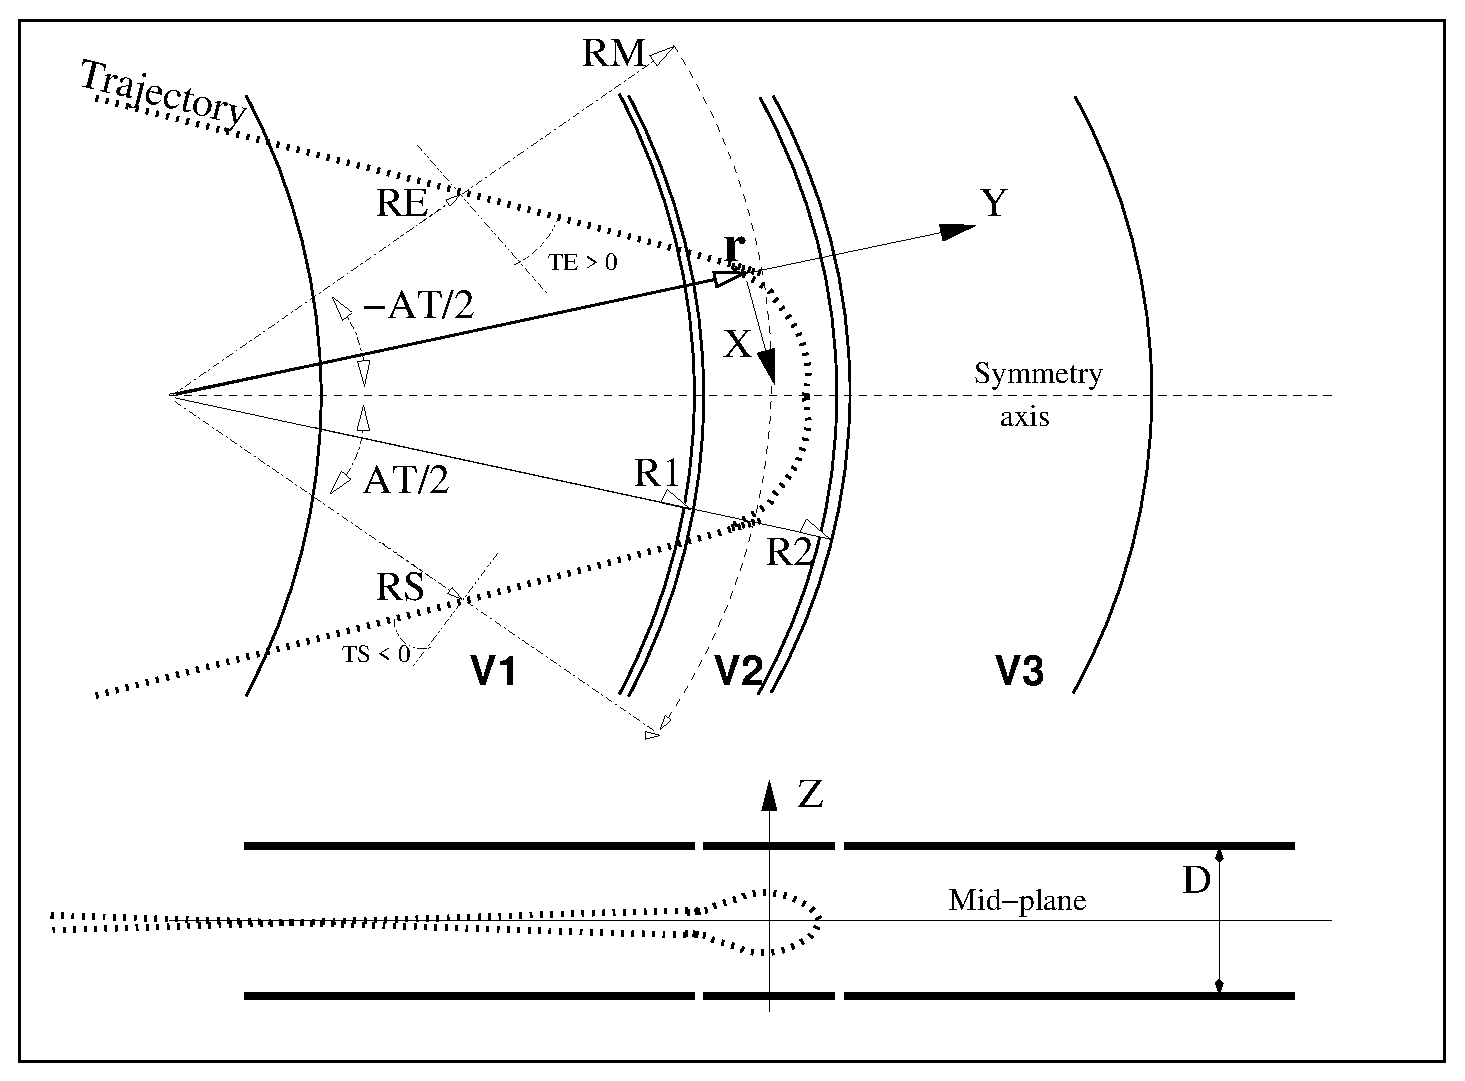
\includegraphics[height=10cm]{FigELMIRC.eps}}
\caption{\label{figELMIRC} \CapELMIRC}
\end{figure}

\vfill


\newpage

\subsubsection*{ELMULT~: \ELMULTTitl} \label{ELMULT}\index{ELMULT|textbf}
\medskip

The simulation of multipolar electric  field $ \vec  M_E $ proceeds by addition of 
the dipolar $ (\vec  E1) $,  quadrupolar ($ \vec  E2 $), sextupolar ($ \vec  E3 $), 
etc.,  up to 20-polar $ (\vec  E10) $ components, and of their derivatives up to fourth 
order, following

\begin{align*}
	\vec  M_E & = \vec  E1 + \vec  E2 + \vec  E3 + ~...~ + \vec  E10 \\
	\dfrac{ \partial\vec  M_E }{ \partial X}  
	          & =  \dfrac{ \partial\vec  E1 }{ \partial X} +
	               \dfrac{\partial\vec  E2 }{ \partial X} + 
	               \dfrac{\partial\vec  E3 }{ \partial X} +
	                         ~...~ +
	               \dfrac{\partial\vec  E10 }{ \partial X}  \\
	\dfrac{ \partial^ 2M_E}{ \partial X\partial Z} 
	          &   = \dfrac{\partial^ 2\vec  E1 }{ \partial X\partial Z} +
	               \dfrac{\partial^ 2\vec  E2 }{\partial X\partial Z} + 
	               \dfrac{\partial^ 2\vec  E3 }{ \partial X\partial Z} +
                                 ~...~ +
	               \dfrac{\partial^ 2\vec  E10 }{ \partial X\partial Z}  \\
	   \text{etc.} &
\end{align*}

\noindent The independent components $ \vec  E1 $ to $ \vec  E10 $ and their
derivatives up to the fourth  order are calculated by differentiating the general multipole potential 
 given  in eq.~\ref{eq2-3-5} (page~\pageref{eq2-3-5}), followed by 
  a $ \dfrac{\pi }{ 2n} $ rotation about the $ X$-axis, so
that the so defined right electric multipole of order $ n$,  and of 
strength~\cite{Biblio14, Biblio15}   %% [14, 15]

$$ K_n = \dfrac{1 }{ 2}\, \dfrac{\gamma }{ \gamma^ 2-1}\, \dfrac{V_ n }{ R^n_0} $$
%
$ (V_ n $ = potential at the electrode, $ R_0 $ = radius at pole tip, 
$\gamma$  = relativistic Lorentz factor of the particle) has the same focusing effect 
 as  the right magnetic multipole of order $ n $ and strength
 $ K_n= \dfrac{B_n }{ R^{n-1}_0 \Br} $ 
$ (B_n $ = field at pole tip, $ \Br $ = particle rigidity, see \textsl{MULTIPOL\index{MULTIPOL}}). 

%\noindent Such $ \dfrac{\pi }{ 2n} $ rotation of the multipole components is
%obtained following the procedure described in section~\ref{sec2.5.3}.  

\medskip

\noindent The entrance and exit fringe fields are treated separately.  They
are characterized by the integration zone $ X_E $ at entrance and $ X_S $ at exit,
as for \textsl{QUADRUPO\index{QUADRUPO}}, and by the extent $ \lambda_ E $ at entrance, $\lambda_ S $ 
at exit. The fringe field extents for the dipole component are $ \lambda_ E $
and $ \lambda_ S $. The fringe field extent for the quadrupolar (sextupolar,  ..., 
 20-polar) component is given by a coefficient $ E_2 $ 
 ($E_3$, ..., $E_{10}$)   at entrance, and $ S_2 $ ($ S_3$, ..., $S_{10}$)   at exit, 
 such that the fringe field extent is $ \lambda_ E\ast E_2$  
 ($\lambda_ E\ast E_3$, ..., $\lambda_ E\ast E_{10}$)  at 
entrance and $ \lambda_ S\ast S_2 $  ($\lambda_ S\ast S_3$, ..., $\lambda_ S\ast S_{10}$) 
 at exit.  
\medskip

\noindent If $ \lambda_ E=0 $  ($\lambda_ S=0$)  the multipole lens is
considered to have a sharp edge field at entrance (exit), and then, 
$ X_E \ (X_S) $ is forced to zero (for the mere purpose of saving computing time).  
\medskip

\noindent If $ E_i=0 $  ($S_i=0$) ($i=2,\, 10$), the entrance (exit) fringe field for
multipole component $ i $ is considered as a sharp edge field.  

\medskip

\noindent Any multipole component $ \vec  Ei $ can be rotated
independently by an angle $ RXi $ around the longitudinal $ X$-axis, for the simulation of 
positioning defects, as well as skew lenses. 

\noindent Use \textsl{PARTICUL\index{PARTICUL}} prior to \textsl{ELMULT}, for the
 definition of particle mass and charge.

\vfill

%%%%%%%%%%%%%%figure%%%%%%%%%%%%%%
\begin{figure}[H]
%\vspace{19 truecm}
%%%Figure 21
\centerline{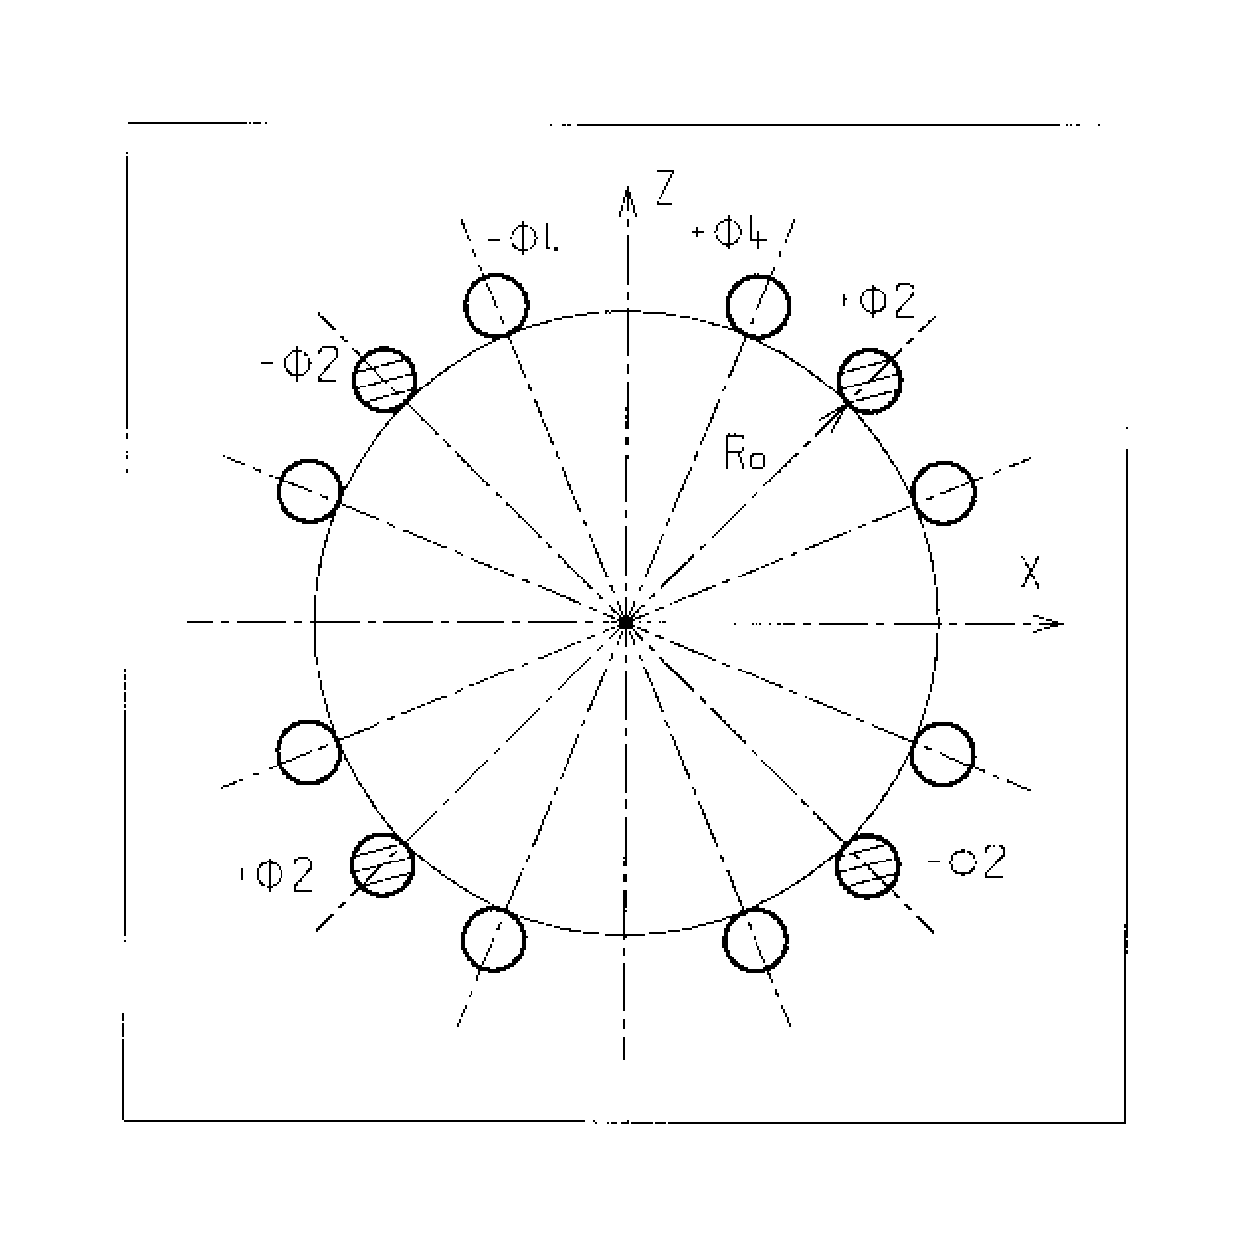
\includegraphics[width=14cm]{Fig21.ps}}
{\setlength{\captionwidth}{13cm}
\hangcaption[Fig21]{\label{fig21}An electric multipole combining skew-quadrupole $ (\vec  E2 \ne \vec 0,~ \vec R2 = \pi/4)$ and  
skew-octupole $ (\vec  E4 \ne \vec 0,~ \vec R4 = \pi/8) $ components 
 ($\vec E1=\vec  E3=\vec  E5= \ ...\ = \vec  E10= \vec 0 $)~\protect\cite{Biblio15}. }   
}\end{figure}
\vfill










\newpage

\subsubsection*{ELREVOL~: \ELREVOLTitl}  \label{ELREVOL}\index{ELREVOL|textbf}
\medskip

\textsl{ELREVOL}  reads a 1-D axial field map from a storage data file,
whose content must fit the following \FORTRAN\ reading sequence  


{\footnotesize
\begin{verbatim}
	      OPEN (UNIT = NL, FILE = FNAME, STATUS = `OLD' [,FORM='UNFORMATTED'])
	      DO 1 I=1, IX
	         IF (BINARY) THEN 
	            READ(NL) X(I), EX(I)
	         ELSE
	            READ(NL,*) X(I), EX(I)
	         ENDIF 
        1     CONTINUE
\end{verbatim}}%% 
\medskip
  
\noindent where $IX$ is the number of nodes along the (symmetry) $X$-axis, $X(I)$ their 
coordinates, and $EX(I)$ are the values of the $X$ component of the field. $EX$ is 
normalized with \textsl{ENORM} prior to ray-tracing. As well the longitudinal coordinate  X is normalized with 
a  \textsl{XNORM} coefficient (useful to convert to centimeters, the working units in  \zgoubi). 


\medskip

\noindent$X$-cylindrical symmetry is assumed, resulting in $EY$
and $EZ$ taken to be zero on axis. $ \vec  E(X,Y,Z) $ and its derivatives along a particle
trajectory are calculated by means of a 5-points polynomial interpolation followed by second 
order off-axis extrapolation (see sections~\ref{sec2.5.2} and~\ref{sec2.4.1}).  

\medskip

\noindent Entrance and/or exit integration boundaries may be defined in the same way 
as in \textsl{CARTEMES\index{CARTEMES}} by means of the flag $ID$ and coefficients  
$A$, $B$, $C$, $A'$, $B'$, $C'$.  
\medskip

\noindent Use \textsl{PARTICUL\index{PARTICUL}} prior to \textsl{ELREVOL}, for the
 definition of particle mass and charge.



\newpage

\subsubsection*{EMMA~: \EMMATitl} \label{EMMA} \index{EMMA|textbf}
\medskip

\noindent  \textsl{EMMA} is dedicated to the reading and treatment of 2-D or 
3-D Cartesian  mesh field maps representing the EMMA FFAG \index{FFAG} cell quadrupole 
doublet\footnote{The stepwise ray-tracing code Zgoubi is the on-line model 
code for the world’s first non-scaling FFAG experiment.}~\cite{EMMAIPAC10,EMMA}. 

\medskip

\noindent  \textsl{EMMA}  can sum up independent field maps of each of the two quadrupoles, with each its 
scaling coefficient. The two maps can be radially  positioned independently of 
one another at $Y_F$, $Y_D$ respectively, just like the 
actual  \textsl{EMMA} quadrupoles. In particular, 

\medskip

  \textsl{MOD} : operational and map \textsl{FORMAT} reading mode~; 
  
  \textsl{MOD}$\le$19 : Cartesian mesh~; 
  
  \textsl{MOD}$\ge$20 : cylindrical mesh.

\medskip

  \textsl{MOD}=0 : two 2D maps, one representing QF, one reprensenting QD. 
 A single map, superimposition of both, is built prior to tracking
 and used for tracking. 


  \textsl{MOD}=1 : two 2D maps, one representing QF, one reprensenting QD, 
 a resulting single map is devised in the following way~: 
  QF\_new is interpolated from QF with dr=xF, 
  QD\_new is interpolated from QD with dr=xD. 
 A single map, superimposition of both, is built prior to tracking
 and used for tracking. 

%  \textsl{MOD}=22 : a single map, including QF and QD, is read. 
%
%  \textsl{MOD}=24 : field at particle is interpolated from a (QF,QD) pair of maps, closest to  current $(Y_F,Y_D)$ 
%  value, taken from a set of (QF,QD) pairs registered in file FNAME. 


\medskip

\noindent The parameters that move/position the maps, as $(Y_F,Y_D)$, 
                are accessible from the FIT, allowing to  adjust the cell tunes. 


\medskip

\noindent  \textsl{EMMA}    works much like  \textsl{TOSCA}.  Refer to that keyword, and to the \FORTRAN\ file 
\texttt{emmac.f}, for details. 









\newpage


\subsubsection*{FFAG~: \FFAGTitl~\cite{reportNIMFFAG,reportICFAFFAG}} \label{FFAG} \index{FFAG magnet, radial} \index{FFAG|textbf} 
\medskip

\noindent \textsl{FFAG} works much like \textsl{DIPOLES} 
as to the field modelling, apart from the  radial dependence of the field, $B=B_0(r/r_0)^k$, so-called ``scaling''. 
Note that \textsl{DIPOLES} does similar job by using a Taylor $r$-expansion of $B_0(r/r_0)^k$. 

\medskip

\noindent The \textsl{FFAG} procedure allows overlapping of fringe fields of neighboring dipoles, 
thus simulating in some sort the field in a dipole $N$-tuple - as for instance in an FFAG doublet 
or triplet. A detailed application, with 
five dipoles, can be found in Ref.~\cite{reportNIMFFAG}. This is done in the way described below. 

\medskip

\noindent  The dimensioning of the magnet is defined by

\medskip

 \begin{tabular}{>{\sl}l!{~:}l}
	 AT &  total angular aperture \\
	 RM & mean radius used for the positioning of field boundaries\\
 \end{tabular}

\medskip

\noindent For each one of the $N=1$ to (maximum) $5$ dipoles of the  $N$-tuple, 
the two  effective field boundaries (entrance and exit EFBs) from which  the dipole field  is drawn are
defined from geometric boundaries, the shape and position of which are determined by the 
following parameters (in the same manner as in \textsl{DIPOLE}, \textsl{DIPOLE-M})
 (see Fig.~\ref{fig9}-A page~\pageref{fig9}, and Fig.~\ref{figFFAG}) 

\medskip

\begin{tabular}{l!{~:}l}
	$ACN_i$  & arbitrary inner angle, used for EFB's positioning  \\
	$\omega$ &  azimuth of an EFB with respect to  \textsl{ACN}\\
	$\theta$ & angle of an EFB with respect to its azimuth (wedge angle)\\ 
	$R_1$, $R_2$  &  radius of curvature of an EFB\\
	$U_1$, $U_2$  &  extent of the linear part of an EFB  \\
\end{tabular}

\begin{figure}[h]
 \begin{center}
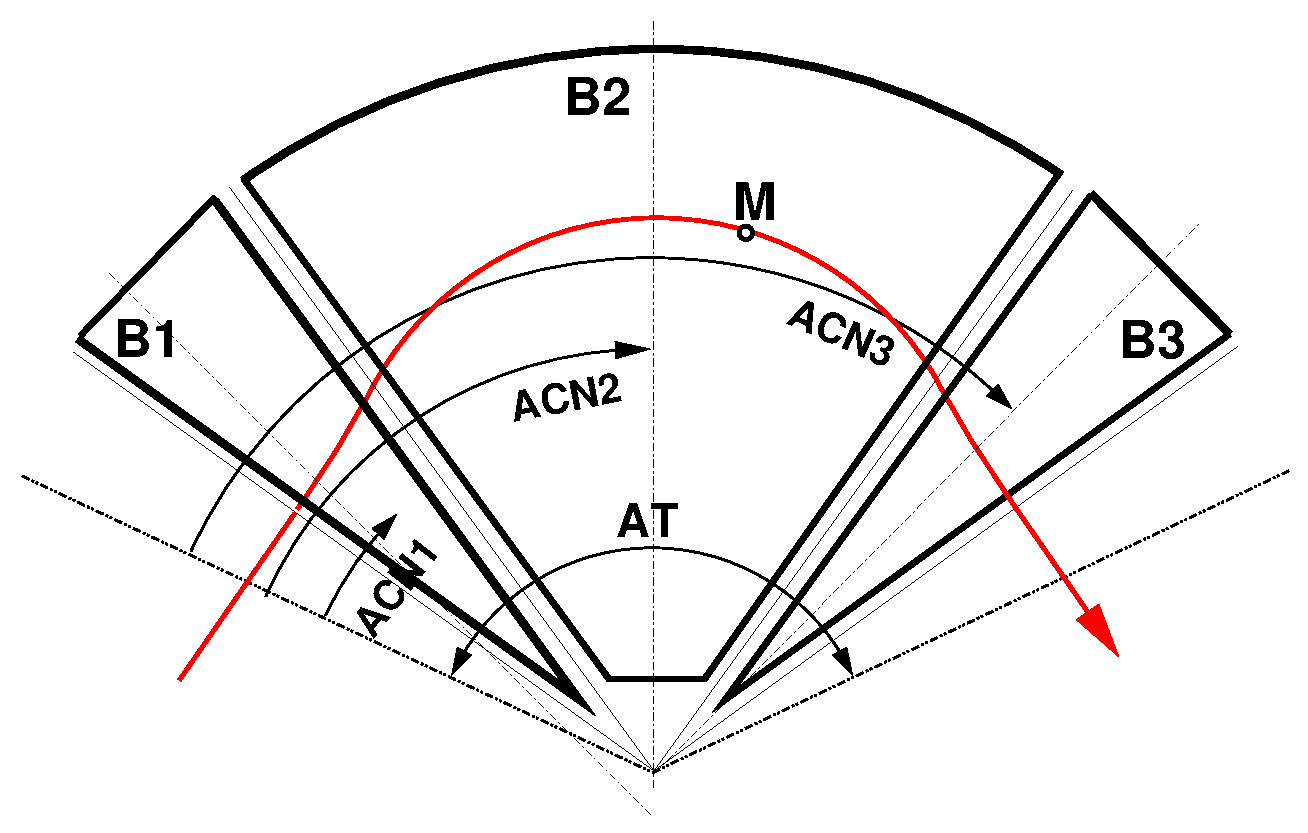
\includegraphics[width=8.5cm]{ffagTriplet.eps}  
{\setlength{\captionwidth}{12cm}
 \hangcaption{ \label{figFFAG}
Definition of a dipole $N$-tuple ($N=3$, a triplet here) using  the \textsl{DIPOLES} or  \textsl{FFAG} \index{FFAG}  procedures. 
}}
  \end{center}
\end{figure}


\paragraph{Calculation of the Field From a Single Dipole} 

 \noindent The magnetic field is calculated in  polar
coordinates.  At all $(R,\theta)$ in the median plane ($z=0$), the 
magnetic field  due  a single one (index $i$) of the  dipoles  of a $N$-tuple FFAG  magnet is written 

$$ \Bz_i(R,\theta) =  \Bz_{0,i} \, \mathcal{F}_i(R,\theta) \, \left(   R/R_M \right)^{K_i}  $$

\noindent wherein $\Bz_{0,i}$  is a reference field, at reference radius  $RM_{i}$, 
 whereas $ \mathcal{F}(R,\theta)$ is calculated as described below. 



\paragraph{Calculation of $\mathcal{F}_i(R,\theta) $} 

\noindent The fringe field coefficient  $\mathcal{F}_i(R,\theta) $ associated with a  dipole is computed as in the 
procedure  \textsl{DIPOLES} (eq.~\ref{EqFFdips}), including (rigorously if the interpolation method is 
used, see page~\pageref{AnalMeth}, or to  order zero if the analytic method is used, see page~\pageref{InterpMeth}) 
 radial dependence of the gap size 

\begin{equation}
\label{EqggvsR}
g(R) = g_0 \, (RM/R)^{\kappa}
\end{equation}
%
\noindent  so to simulate the effect of gap shaping on $ \Bz_i(R,\theta)|_R$ field fall-off,  over the 
all radial extent of a scaling FFAG dipole (with normally - but not 
necessarily in practice - $\kappa \approx K_i$). 
 

\medskip

\paragraph{Calculation of the Field Resulting From All $N$ Dipoles}

For the rest, namely, calculation of the full field at particle position from the $N$ dipoles, 
analytical   calculation or numerical interpolation of the  mid-plane field derivatives, 
extrapolation off median plane, etc., things are performed exactly as in the case of the 
 \textsl{DIPOLES} procedure (see page~\pageref{FFatAP}). 




\medskip

\paragraph{Sharp Edge} 

\noindent Sharp edge field fall-off at a field boundary  can only be simulated if the following conditions are fulfilled~: 

- entrance (resp. exit)  field boundary  coincides with entrance (resp. exit) 
dipole limit (it means in particular, see Fig.~\ref{fig9},  
$\omega^+= ACENT$ (resp. $\omega^- = -(AT-ACENT)$), 
together with $\theta=0$ at entrance (resp. exit) EFBs), 

- analytical method for calculation of the  mid-plane field derivatives is used. 







\newpage


\subsubsection*{FFAG-SPI~: \FFAGSPITitl~\cite{reportICFAFFAG,reportNIMFFAGSPI}} \label{FFAG-SPI} \index{FFAG magnet, spiral} \index{FFAG-SPI|textbf} 
\medskip

\noindent \textsl{FFAG-SPI} works much like \textsl{FFAG} as to the field modelling, 
with essentially a different axial  dependence. 

\medskip

\noindent The \textsl{FFAG-SPI} procedure allows overlapping of fringe fields of neighboring dipoles, 
thus simulating in some sort the field in a dipole $N$-tuple  (similar to Fig.~\ref{figFFAG}, page~\pageref{figFFAG}).
This allows  for instance accounting for fringe field effects, or clamps, as schemed in 
Fig.~\ref{figFFAGSPI}. 

\medskip

\noindent  The dimensioning of the magnet is defined by

\medskip

 \begin{tabular}{>{\sl}l!{~:}l}
	 AT &  total angular aperture \\
	 RM & mean radius used for the positioning of field boundaries\\
 \end{tabular}

\medskip

\noindent For each one of the $N=1$ to (maximum) $5$ dipoles of the  $N$-tuple, 
the two  effective field boundaries (entrance and exit EFBs) from which  the dipole field  is drawn are
defined from geometric boundaries, the shape and position of which are determined by the 
following parameters 

\medskip

\begin{tabular}{l!{~:}l}
	$ACN_i$  & arbitrary inner angle, used for EFB's positioning  \\
	$\omega$ &  azimuth of an EFB with respect to  \textsl{ACN}\\
	$\xi$ & spiral angle \\
\end{tabular}

\medskip

\noindent with $ACN_i$ and $\omega$ as defined in Fig.~\ref{figFFAGSPI} 
(similar to what can be found in Figs.~\ref{figFFAG} and \ref{fig9}-A). 

\begin{figure}[h]
\centerline{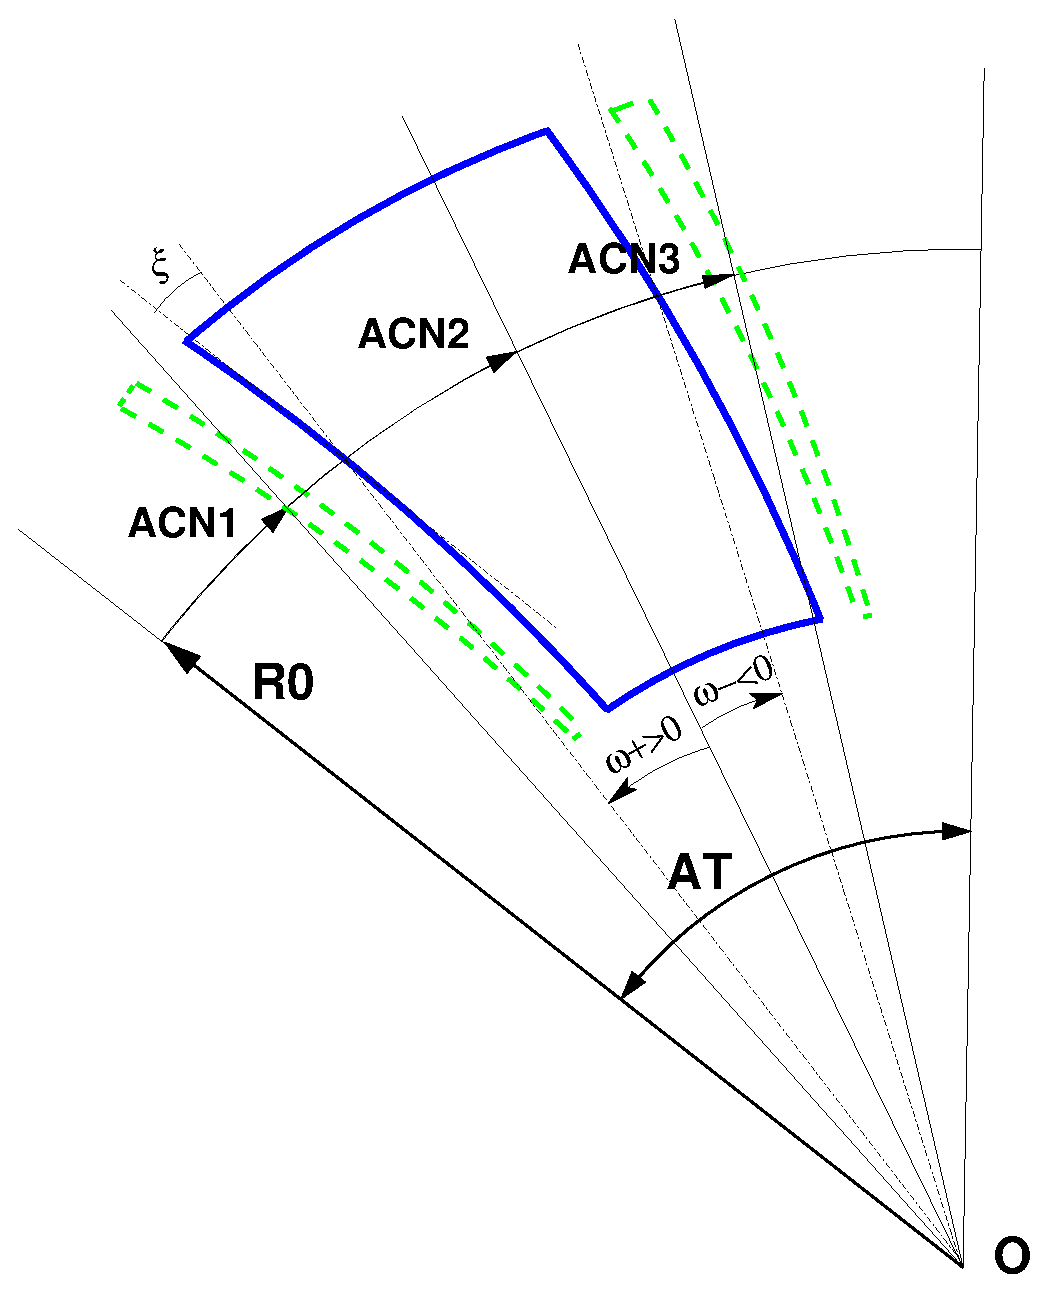
\includegraphics[width=7cm]{figFFAGSPI.eps}  }
{\setlength{\captionwidth}{12cm}
 \hangcaption[Fig29a]{ \label{figFFAGSPI}
A $N$-tuple spiral sector FFAG magnet \index{FFAG}  ($N=3$ here, simulating active field clamps at 
entrance and exit side of a central dipole). 
}}
\end{figure}


\medskip


\paragraph{Calculation of the Field From a Single Dipole} 

 \noindent The magnetic field is calculated in  polar
coordinates.  At all $(R,\theta)$ in the median plane ($Z=0$), the 
magnetic field  due  a single one (index $i$) of the  dipoles  of a $N$-tuple spiral FFAG  magnet is written 

$$ \Bz_i(R,\theta) =  \Bz_{0,i} \, \mathcal{F}_i(R,\theta) \, \left(   R/R_M \right)^{K_i}  $$

\noindent wherein $\Bz_{0,i}$  is a reference field, at reference radius  $RM_{i}$, 
 whereas $ \mathcal{F}(R,\theta)$ is calculated as described below. 



\paragraph{Calculation of $\mathcal{F}_i(R,\theta) $} 

\noindent The fringe field coefficient  $\mathcal{F}_i(R,\theta) $ associated with a  dipole is computed as in the 
procedure  \textsl{DIPOLES} (eq.~\ref{EqFFdips}), including  radial dependence of the gap size 

\begin{equation}
%\label{EqggvsR}
g(R) = g_0 \, (RM/R)^{\kappa}
\end{equation}
%
\noindent  so to simulate the effect of gap shaping on $ \Bz_i(R,\theta)|_R$ 
field fall-off,  over the 
all radial extent of the  dipole (with normally - yet not necessarily in practice - $\kappa \approx K_i$). 
 

\medskip

\paragraph{Calculation of the Full Field From All $N$ Dipoles}

For the rest, namely calculation of the full field at particle position, as resulting from the $N$ dipoles,  
  calculation of the  mid-plane field derivatives, 
extrapolation off median plane, etc., things are performed in the same manner  as for the 
 \textsl{DIPOLES} procedure (see page~\pageref{FFatAP}). 





\newpage

\subsubsection*{MAP2D~: \MAPTwoDTitl~\cite{Pavel}} \label{MAP2D} \index{MAP2D|textbf}
\medskip

\textsl{MAP2D} reads a 2-D field map that provides the three
components $ B_X$, $ B_Y $, $ B_Z $ of the magnetic field at all nodes of a 2-D Cartesian 
uniform mesh in an $(X,Y)$ plane. 
No particular symmetry is assumed, which allows the 
treatment of any type of field (\emph{e.g.}, solenoidal, or dipole,  
helical dipole, at  arbitrary $Z$ elevation 
- the map needs not be a mid-plane map). 

\medskip

\noindent The field map data file has to be be filled with a 
format that satisfies the  \FORTRAN\ reading sequence below (in principle compatible 
with \textsl{TOSCA} code outputs), details and possible updates are to be found in the source  
file \texttt{'fmapw.f'}~:  

{\footnotesize
\begin{verbatim}
	      OPEN (UNIT = NL, FILE = FNAME, STATUS = `OLD' [,FORM='UNFORMATTED'])
	       DO 1 J=1,JY 
	          DO 1 I=1,IX
	             IF (BINARY) THEN
	                READ(NL) Y(J), Z, X(I), BY(I,J), BZ(I,J), BX(I,J)
	             ELSE
	                READ(NL,100) Y(J), Z, X(I), BY(I,J), BZ(I,J), BX(I,J)
	100             FORMAT (1X, 6E11.4)
	             ENDIF
      1        CONTINUE
\end{verbatim}}
\medskip

\noindent $IX$ ($JY$) is the number of longitudinal (transverse horizontal) nodes of 
the 2-D uniform mesh, $Z $ is the considered $Z$-elevation of the map. For 
binary files, FNAME must begin with \mbox{`B\_ '} or  \mbox{`b\_'}, a flag `BINARY' will thus be 
set to `.TRUE.'. The field $ \vec  B=(B_X,B_Y,B_Z )$ is next normalized with 
BNORM, prior to ray-tracing.  As well the  coordinates  X, Y~are normalized with 
  \textsl{X-, Y-NORM} coefficients (useful to convert to centimeters, the working units in  \zgoubi). 


\medskip

\noindent At each step of the trajectory of a particle, the field and its 
derivatives are calculated using a second or fourth degree polynomial interpolation followed 
by a $ Z $ extrapolation (see sections~\ref{sec2.3.3} page~\pageref{sec2.3.3},~\ref{sec2.4.3} page ~\pageref{sec2.4.3}). 
The  interpolation grid is 3*3-node for 2nd order (option \textsl{IORDRE = 2\index{IORDRE}}) or 5*5 
for 4th order (option \textsl{IORDRE = 4\index{IORDRE}}). 

\medskip

\noindent Entrance and/or 
exit integration boundaries may be defined, in the same way as for \textsl{CARTEMES\index{CARTEMES}}.




\newpage

\subsubsection*{MAP2D-E~: \MAPTwoDETitl} \label{MAP2D-E} \index{MAP2D-E|textbf}
\medskip

\textsl{MAP2D-E} reads a 2-D field map that provides the three
components $ E_X$, $ E_Y $, $ E_Z $ of the electric field at all nodes of a 2-D Cartesian 
uniform mesh in an $(X,Y)$ plane. 
No particular symmetry is assumed, which allows the 
treatment of any type of field (\emph{e.g.},  field of a parallel-plate mirror with arbitrary $Z$ elevation 
- the map needs not be a mid-plane map). 

\medskip

\noindent The field map data file has to be be filled with a 
format that satisfies the  \FORTRAN\ reading sequence below (in principle compatible 
with \textsl{TOSCA} code outputs), details and possible updates are to be found in the source  
file \texttt{'fmapw.f'}~:  

{\footnotesize
\begin{verbatim}
	      OPEN (UNIT = NL, FILE = FNAME, STATUS = `OLD' [,FORM='UNFORMATTED'])
	       DO 1 J=1,JY 
	          DO 1 I=1,IX
	             IF (BINARY) THEN
	                READ(NL) Y(J), Z, X(I), EY(I,J), EZ(I,J), EX(I,J)
	             ELSE
	                READ(NL,100) Y(J), Z, X(I), EY(I,J), EZ(I,J), EX(I,J)
	100             FORMAT (1X, 6E11.4)
	             ENDIF
      1        CONTINUE
\end{verbatim}}
\medskip

\noindent $IX$ ($JY$) is the number of longitudinal (transverse horizontal) nodes of 
the 2-D uniform mesh, $Z$ is the considered $Z$-elevation of the map.   For 
binary files, FNAME must begin with \mbox{`E\_ '} or  \mbox{`b\_'}, a flag  `BINARY' will thus be 
set to `.TRUE.'. The field $ \vec  E=(E_X,E_Y,E_Z )$ is next normalized with 
ENORM, prior to ray-tracing.  As well the coordinates  X, Y are normalized with 
  \textsl{X-,Y-NORM} coefficients (useful to convert to centimeters, the working units in  \zgoubi. 


\medskip

\noindent At each step of the trajectory of a particle, the field and its 
derivatives are calculated using a second or fourth degree polynomial interpolation followed 
by a $ Z $ extrapolation (see sections~\ref{sec2.3.3} page~\pageref{sec2.3.3},~\ref{sec2.4.3} page ~\pageref{sec2.4.3}). 
 The interpolation grid is 3*3-node for 2nd order (option \textsl{IORDRE = 2\index{IORDRE}}) or 5*5 
for 4th order (option \textsl{IORDRE = 4\index{IORDRE}}). 

\medskip

\noindent Entrance and/or 
exit integration boundaries may be defined, in the same way as for \textsl{CARTEMES\index{CARTEMES}}.




\newpage

\subsubsection*{MARKER~: \MARKERTitl} \label{MARKER} \index{MARKER|textbf}
\medskip

\textsl{MARKER} does nothing. Just a marker. No data. 

\bigskip

As any other keyword, \textsl{MARKER} is allowed two \LABEL s. Using 
 '.plt' as a second \LABEL\ will cause storage of current coordinates into 
zgoubi.plt\index{LABEL@{\LABEL}}\index{zgoubi.plt}. 





\newpage

\subsubsection*{MULTIPOL~:  \MULTIPOLTitl} \label{MULTIPOL}\index{MULTIPOL|textbf}
\medskip 

The simulation of  multipolar magnetic field $ \vec  M $ by \textsl{MULTIPOL}  proceeds 
by addition of the dipolar  ($\vec  B1$),  quadrupolar ($ \vec  B2 $), sextupolar 
($ \vec  B3 $), etc., up to 20-polar  ($\vec  B10$) 
components, and of their derivatives up to fourth order, following

\begin{align*}
	\vec  M &   =   \vec B1+\vec  B2+\vec  B3+ \ ...\ +\vec  B10  \\ 
	\dfrac{ \partial\vec M }{ \partial X} 
	        &   = \dfrac{ \partial\vec  B1}{ \partial X} + 
	        \dfrac{\partial\vec  B2 }{ \partial X} + 
	        \dfrac{\partial\vec  B3}{ \partial X} + 
                            \ ...\ +
	        \dfrac{\partial\vec  B10 }{ \partial X} \\
	\dfrac{ \partial^ 2\vec  M }{ \partial X\partial Z} 
	       & = \dfrac{ \partial^ 2\vec  B1 }{ \partial X\partial Z} + 
	       \dfrac{\partial^ 2\vec  B2 }{ \partial X\partial Z} + 
	       \dfrac{\partial^ 2\vec  B3}{ \partial X\partial Z} + 
                            \ ...\ +
 	       \dfrac{\partial^ 2\vec  B10}{ \partial X\partial Z} \\
	\text{etc. } &
\end{align*}


\noindent The independent components $ \vec  B1$, $\vec  B2$, $\vec  B3$, ..., 
$ \vec  B10 $  and their derivatives up to the fourth order are calculated as described in 
 section~\ref{sec2.3.5}.  

\medskip

\noindent The entrance and exit fringe fields are treated separately.  They
are characterized by the integration zone $ X_E $ at entrance and $ X_S $ at exit,
as for \textsl{QUADRUPO\index{QUADRUPO}}, and by the extent $ \lambda_ E $ at entrance, 
$\lambda_ S $ at exit. The fringe field extents for the dipole component are $ \lambda_ E $ 
and $ \lambda_ S $. The fringe field for the quadrupolar 
(sextupolar,  ..., 20-polar) component is given by a coefficient $ E_2 $ 
 ($E_3$, ..., $E_{10}$)  at entrance, and 
$ S_2 $ ($ S_3$, ..., $S_{10}$)  at exit, such that the extent is $ \lambda_ E\ast E_2$
 ($\lambda_ E\ast E_3$, ..., $\lambda_ E\ast E_{10}$)  at 
entrance and $ \lambda_ S\ast S_2 $  ($\lambda_ S\ast S_3$, ..., $\lambda_ S\ast S_{10}$)  
at exit. 
\medskip

\noindent If $ \lambda_ E=0 $  ($\lambda_ S=0$)  the multipole lens is
considered to have a sharp edge field at entrance (exit), and then, $ X_E \ (X_S) $ is forced to zero 
(for the mere purpose of saving computing time).  If $ E_i=0 $  ($S_i=0$) ($i=2,\, 10$), the entrance (exit) fringe field for 
 the multipole component $ i $ is considered as a sharp edge field.  
In sharp edge field model, the wedge angle vertical first order focusing effect (if $\vec  B1$ is non zero) is simulated at magnet entrance and exit  by a kick $P_2 = P_1 - Z_1 \tan (\epsilon / \rho)$ applied to each particle ($P_1$, $P_2$ are the vertical angles upstream and downstream of the EFB, $Z_1$ is the vertical particle position at the EFB, $\rho$ the local horizontal bending radius and $\epsilon$ the wedge angle experienced by the particle~; $\epsilon$ depends on the horizontal angle T). 

\medskip

\noindent Any multipole component $ \vec  Bi $ can be rotated independently
by an angle $ RXi $ around the longitudinal $ X$-axis, for the simulation of positioning defects,
as well as skew lenses. 

\medskip

\noindent Magnet (mis-)alignment is assured by \textsl{KPOS}. 
\textsl{KPOS} also  allows some degrees of automatic alignment useful for periodic structures (section~\ref{sec4.6.2}).



\newpage

\subsubsection*{OCTUPOLE~: \OCTUPOLETitl\  (Fig.~\protect\ref{fig24}) } \label{OCTUPOLE} \index{OCTUPOLE|textbf} 
\medskip 

 The meaning of parameters for \textsl{OCTUPOLE} is the same as for 
\textsl{QUADRUPO\index{QUADRUPO}}.  In fringe field regions the magnetic field $ \vec  B(X,Y,Z)$ and 
its derivatives up to fourth order are derived from the scalar potential 
approximated to the 8-th order in $ Y $ and $ Z $

\begin{align*}
	V(X,Y,Z) &   =   \left(G-\dfrac{G^{\prime\prime} }{ 20} \, (Y^2+Z^2)+
	              \dfrac{G^{\quaprime} }{ 960}\, (Y^2+Z^2)^2 \right) (Y^3Z-YZ^3)   \\
	\text{with } ~ G_0 &   =  \dfrac{ B_0 }{ R^3_0} 
\end{align*}

\noindent The  modelling of the fringe field form factor  $G(X)$
 is described under \textsl{QUADRUPO}, p.~\pageref{QUADRUPO}. 

\medskip

\noindent Outside fringe field regions, or everywhere in sharp edge dodecapole
($ \lambda_ E=\lambda_ S=0$) , $ \vec  B(X,Y,Z) $ in the magnet is given by 

\begin{align*}
	B_X &   =   0 \\
	B_Y &   =   G_0(3Y^2-Z^2)\, Z  \\
	B_Z &   = G_0(Y^2-3Z^2) \, Y    
\end{align*}
\vfill

%%%%%%%%%%%%%%figure%%%%%%%%%%%%%%
\begin{figure}[H]
%\vspace{12 truecm}
%%%Figure 24
\centerline{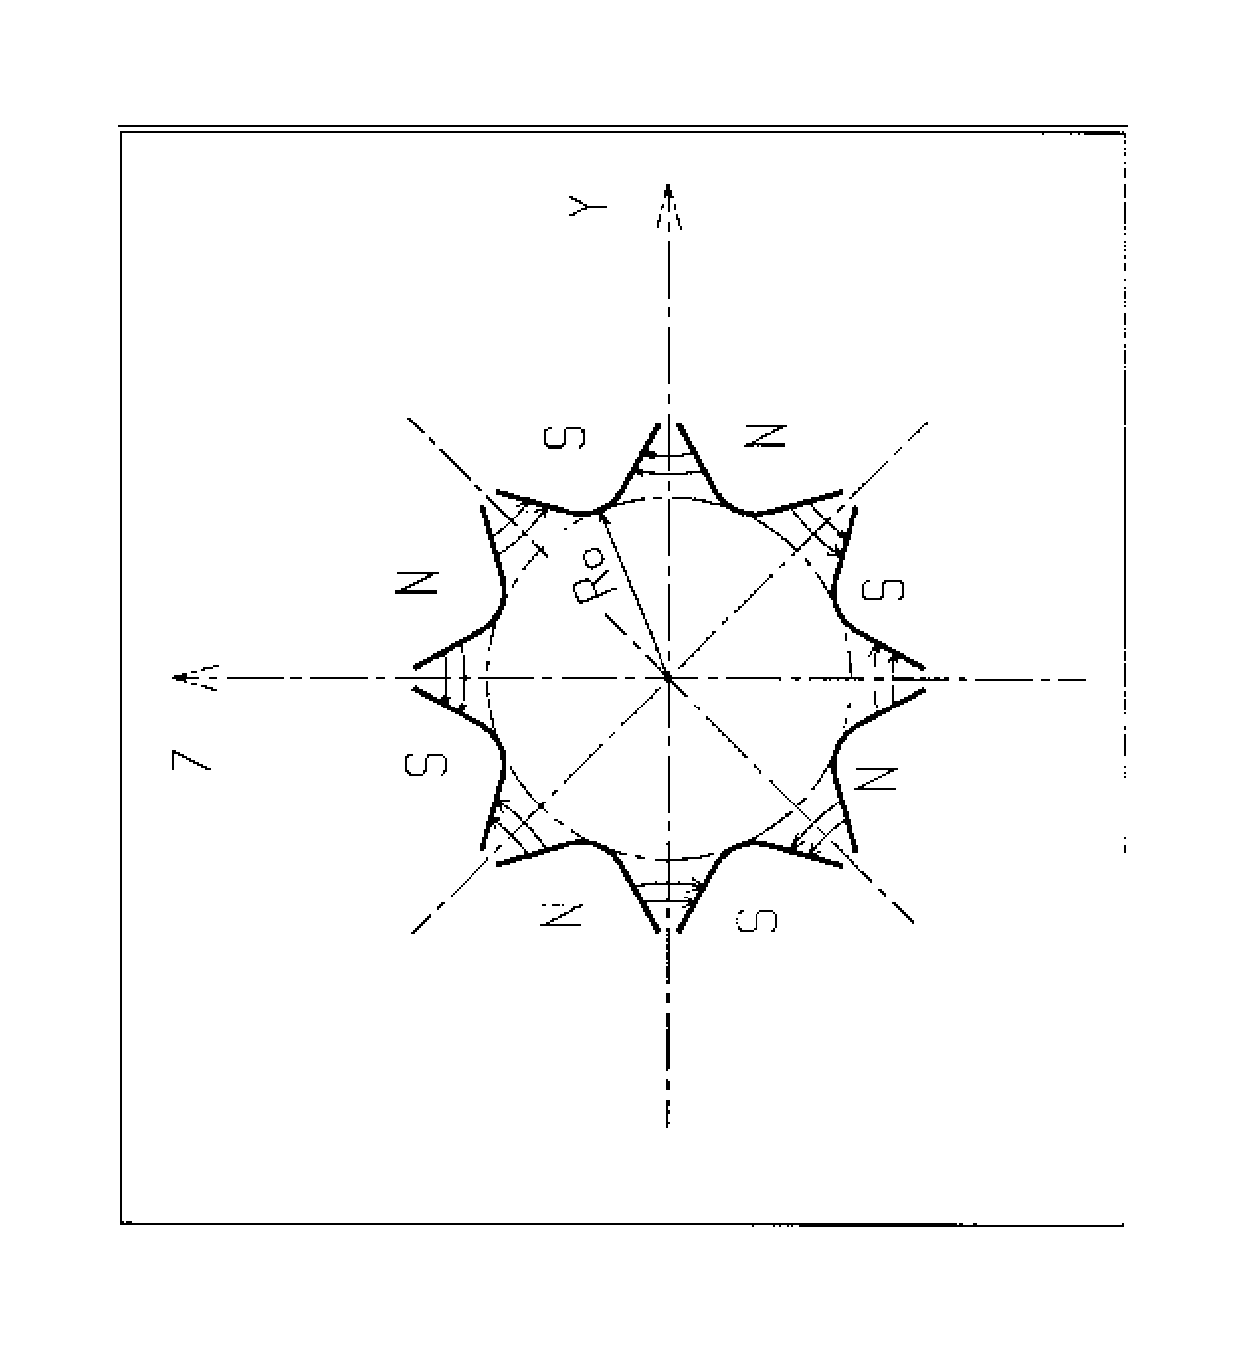
\includegraphics[height=12cm,angle=-90]{Fig24.ps}}
\caption{\label{fig24}Octupole magnet}
\end{figure}
\vfill

\newpage

\subsubsection*{POISSON~:\POISSONTitl} \label{POISSON} \index{POISSON|textbf}
\medskip 

This keyword allows reading a field profile $ B(X) $ from  \textsl{POISSON} output. 
Let \textsl{FNAME} be the name of this output file (normally,
\textsl{FNAME} = outpoi.lis\index{outpoi.lis})~; 
the data are read following the \FORTRAN\ statements here under 

{\footnotesize
\begin{verbatim}
	 I = 0
   11    CONTINUE
	   I = I + 1
           READ(LUN,101,ERR=10,END=10) K, K, K, R, X(I), R, R, B(I) 
   101     FORMAT(I1, I3, I4, E15.6, 2F11.5, 2F12.3)
         GOTO 11     
   10    CONTINUE
         ...
\end{verbatim}}
\medskip
 
\noindent where X(I) is the longitudinal coordinate, and B(I) is the Z
component of the field at a node (I) of the mesh. K's and R's are dummy variables 
appearing in the \textsl{POISSON} output file outpoi.lis
 but not used here. 
\medskip

\noindent From this field profile, a 2-D median plane map is built, with a 
rectangular and uniform mesh~; mid-plane symmetry is assumed. The field at 
each node $ (X_i,Y_j) $ of the map is $ B(X_i) $, independent of $ Y_j $
(\emph{i.e.}, the distribution is uniform in the $ Y $ direction).  
\medskip

\noindent For the rest, \textsl{POISSON} works in a way similar to \textsl{CARTEMES\index{CARTEMES}}. 

\newpage
\subsubsection*{POLARMES~: \POLARMESTitl} \label{POLARMES} \index{POLARMES|textbf}
\medskip 

Similar to \textsl{CARTEMES\index{CARTEMES}}, apart from the polar 
mesh frame~: $IX$ is the number of angular nodes, $JY$ the number of 
radial nodes~; $X(I)$ and $Y(J)$ are respectively the angle and radius 
of a node (these parameters are similar to those entering in the 
definition of the field map in \textsl{DIPOLE-M}\index{DIPOLE-M}).

\newpage

\subsubsection*{PS170~: \PSusoTitl} \label{PS170} \index{PS170|textbf}
\medskip 

\textsl{PS170} is dedicated to a `rough' simulation
of CERN \textsl{PS170} spectrometer dipole.  
\medskip

\noindent The field $ B_0 $ is constant inside the magnet, and zero outside. 
The pole is a circle  of radius $ R_0 $, centered on the $ X $ axis.  The output coordinates are
generated at the distance \XL\ from the entrance (Fig.~\ref{fig25}).  %%%
\vfill

%%%%%%%%%%%%%%figure%%%%%%%%%%%%%%
\begin{figure}[H]
%\vspace{17 truecm}
%%%Figure 25
\centerline{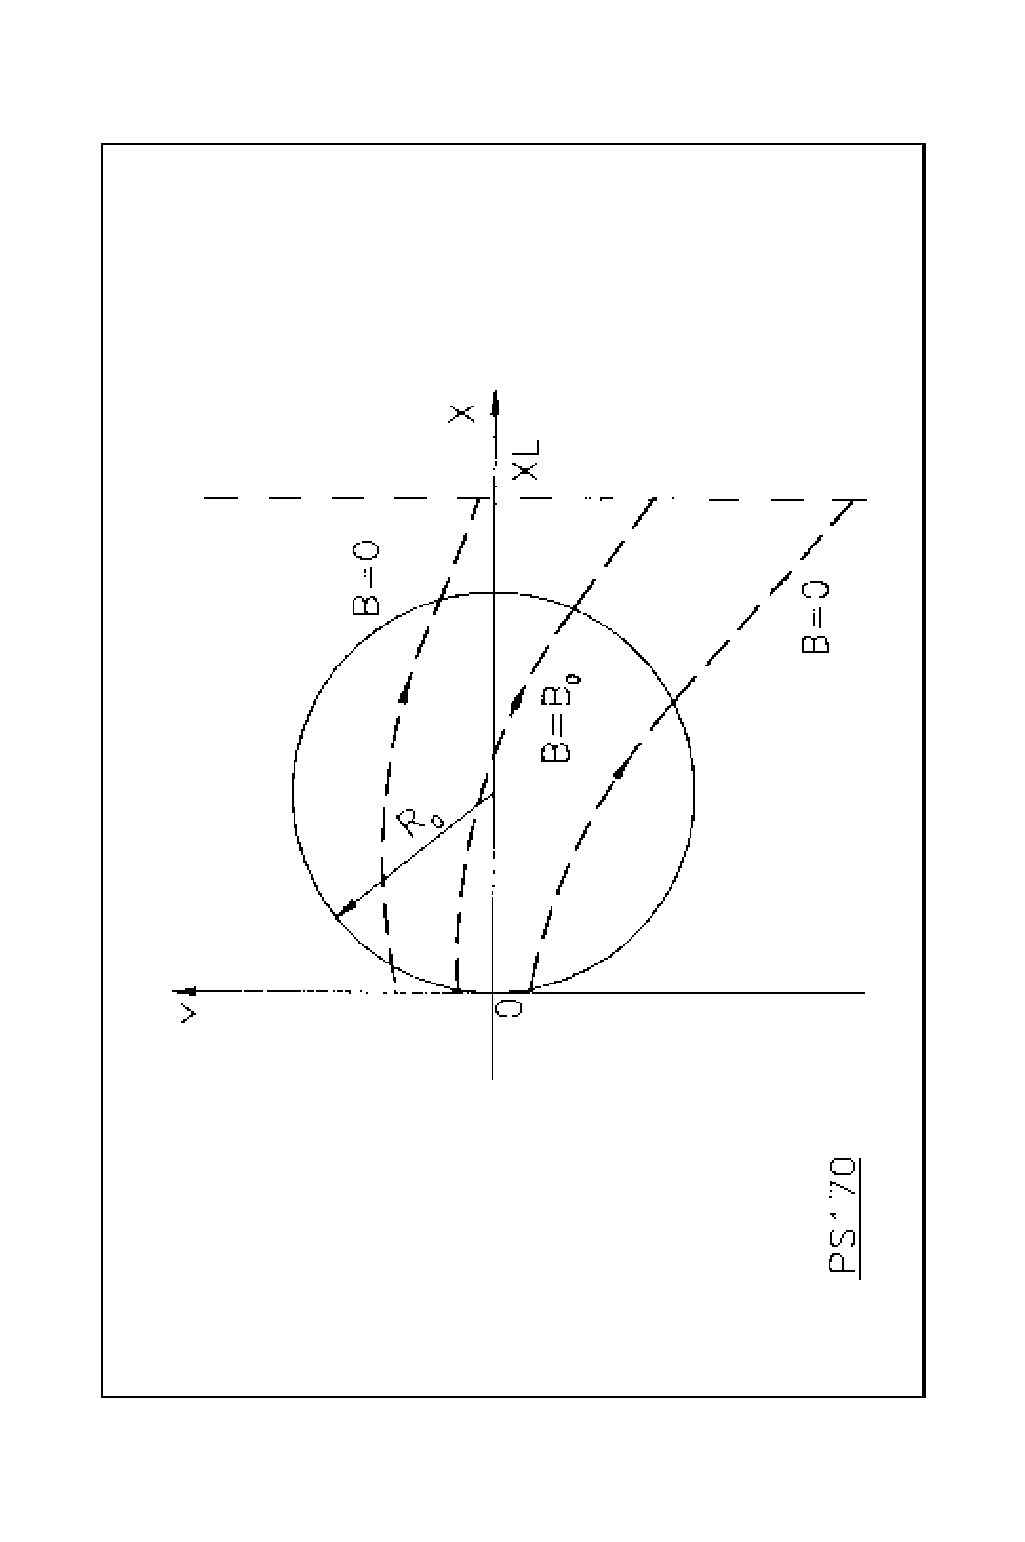
\includegraphics[height=15cm,angle=-90]{Fig25.ps}}
\caption{\label{fig25}Scheme of the PS170 magnet simulation.}
\end{figure}

\vfill

\newpage

\subsubsection*{QUADISEX, SEXQUAD~: \QUADISEXTitl} \label{QUADISEX}\label{SEXQUAD}
\medskip 
\index{QUADISEX|textbf} \index{SEXQUAD|textbf}

\textsl{SEXQUAD}    defines in a simple way a sharp edge field with quadrupolar, 
sextupolar and octupolar components. \textsl{QUADISEX}  adds a dipole component. The length of 
the element is $ \XL $.  The vertical component $ B \equiv B_Z(X,Y,Z=0) $ of the field and its derivatives in median plane are 
calculated at each step using the following expressions 

\begin{align*}
	B &   =     B_0
	           \left(U+ \dfrac{N }{ R_0}Y + 
	                \dfrac{B }{ R^2_0} Y^2+ \dfrac{G }{ R^3_0} Y^3 \right)  \\
	\dfrac{ \partial B }{ \partial Y} 
	   &   =   B_0 \left(
	             \dfrac{N }{ R_0} + 2 \dfrac{B }{ R^2_0} Y + 3\dfrac{G }{ R^3_0}Y^2 \right) \\  
	\dfrac{ \partial^ 2B }{ \partial Y^2} 
	  &  =     B_0 \left(2 \dfrac{B }{ R^2_0} + 6\dfrac{G }{ R^3_0} Y \right) \\
	\dfrac{ \partial^ 3B }{ \partial Y^3}  
	   & =     6B_0 \,  \dfrac{G }{ R^3_0}
\end{align*}  
   %
    and then extrapolated out of the median plane by Taylor expansion in $ Z $ 
(see section~\ref{sec2.3.2}).
\medskip

\noindent With option \textsl{SEXQUAD}, $ U=0$,  while with \textsl{QUADISEX}, $U=1 $. 

\newpage

\subsubsection*{QUADRUPO~:  \QUADRUPOTitl\  (Fig.~\protect\ref{fig26}) } \label{QUADRUPO} \index{QUADRUPO|textbf}
\medskip

The length of the magnet $ \XL $ is the distance between the
effective field boundaries (EFB), Fig.~\ref{fig27}. The field at the pole tip $ R_0 $ is $ B_0 $. 

\noindent The extent of the  entrance (exit) fringe field is characterized by 
$ \lambda_ E(\lambda_ S) $.  The distance of ray-tracing on both sides of the
EFB's, in the field fall off regions, will be $\pm$  $ X_E $ at 
the entrance, and $\pm$  $ X_S $ at the exit (Fig.~\ref{fig27}),  
by prior and further automatic change of frame. 

\noindent In the fringe field  regions $[ -X_E,X_E ]$  and 
$[ -X_S,X_S ]$ on both sides of the EFB's, $ \vec  B(X,Y,Z) $ and its derivatives up to
fourth order are calculated at each step of the trajectory from the analytical expressions 
of the three components $ B_X $, $ B_Y $, $ B_Z $ obtained by differentiation
of the scalar potential (see section~\ref{sec2.3.5}) expressed to the 8th order in $ Y $ 
and $ Z $. 

 \begin{gather*}
 	V(X,Y,Z)     =   \left(G- \dfrac{G^{\prime\prime} }{ 12}\, (Y^2+Z^2)+
	             \dfrac{G^{\quaprime} }{ 384}\, (Y^2+Z^2)^2-
	             \dfrac{G^{\cinqprime\prime} }{ 23040}\, (Y^2+Z^2)^3 \right)YZ  \\
	(\quad G^{\prime\prime} =d^2G/dX^2,...) \\
\intertext{where $ G $ is the gradient on axis~\protect\cite{Biblio12}~:  } %% [12]
    G(s) = \dfrac{G_0 }{ 1+ \exp  P(s)}\qquad \text{with} \quad G_0=\dfrac{B_0}{R_0} \\
\intertext{and,}
     P(s) = C_0
       +C_1 \left(  \dfrac{s }{ \lambda} \right) 
       +C_2 \left( \dfrac{s }{ \lambda} \right)^2 
       + C_3 \left( \dfrac{s }{ \lambda} \right)^3 
       +C_4 \left( \dfrac{s }{ \lambda} \right)^4 
       + C_5 \left(\dfrac{s }{ \lambda} \right)^5
       P(s)=C_0+C_1 \left(\dfrac{s }{ \lambda} \right) + C_2 \left(\dfrac{s }{ \lambda}\right)
\end{gather*}
%
 where, $ s $ is the distance to the field boundary and $\lambda$
stands for $ \lambda_ E $ or $ \lambda_ S $ 
(normally, $ \lambda  \simeq  2  \ast  R_0$). 

\noindent When fringe fields overlap inside the magnet $ (\XL\leq X_E+X_S)$,  
the gradient $ G $ is expressed as 

$$ G = G_E+G_S-1 $$
%
where, $ G_E $ is the entrance gradient and $ G_S $ is the exit gradient. 

\noindent If $ \lambda_ E=0$ ($\lambda_ S=0$),  the field at entrance 
(exit) is considered as sharp edged, and then $ X_E(X_S) $ is forced to zero 
(for the mere purpose of saving computing time). 

\noindent Outside of the fringe field regions (or everywhere when 
$ \lambda_E=\lambda_ S=0$)   $ \vec  B(X,Y,Z) $ in the magnet is given by 

\begin{align*}
	B_X &   =     0 \\
	B_Y &   =    G_0Z \\
	B_Z &   =     G_0Y  
\end{align*}

\newpage

%%%%%%%%%%%%%%figure%%%%%%%%%%%%%%
\begin{figure}[H]
%\vspace{9 truecm}
%%%Figure 26
\centerline{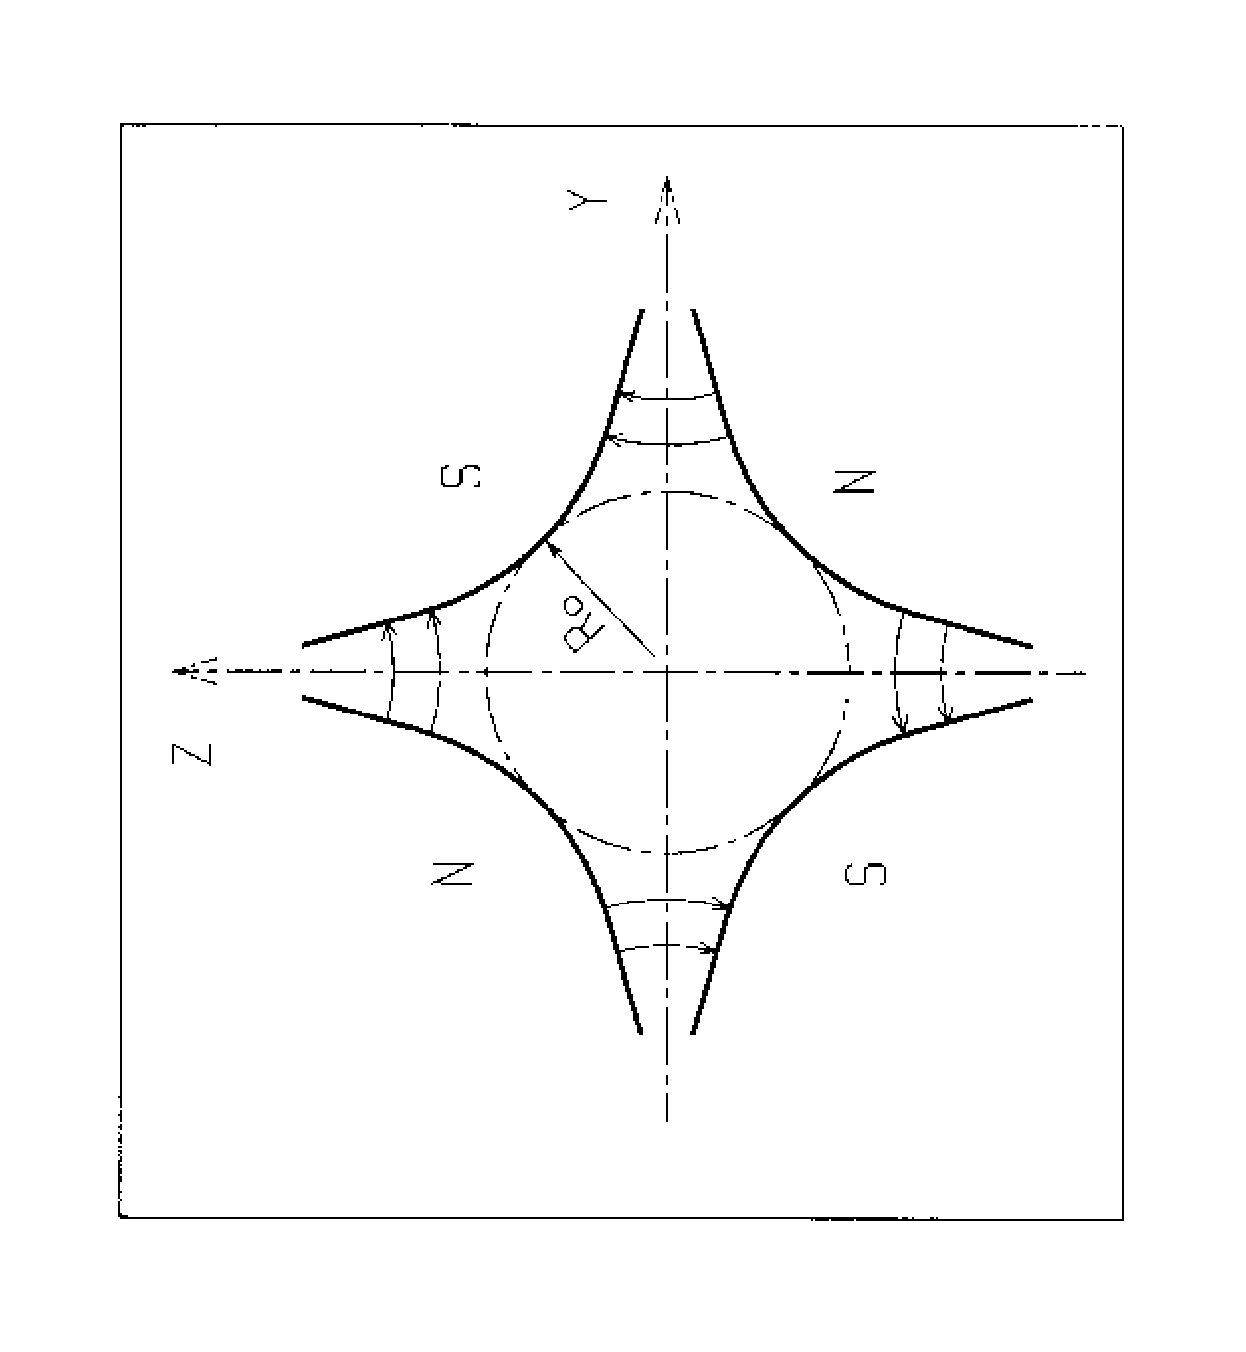
\includegraphics[height=10cm,angle=-90]{Fig26.ps}}
\caption{\label{fig26}Quadrupole magnet}
\end{figure}
\vfill
%%%%%%%%%%%%%%figure%%%%%%%%%%%%%%
\begin{figure}[H]
%\vspace{11 truecm}
%%%Figure 27
\centerline{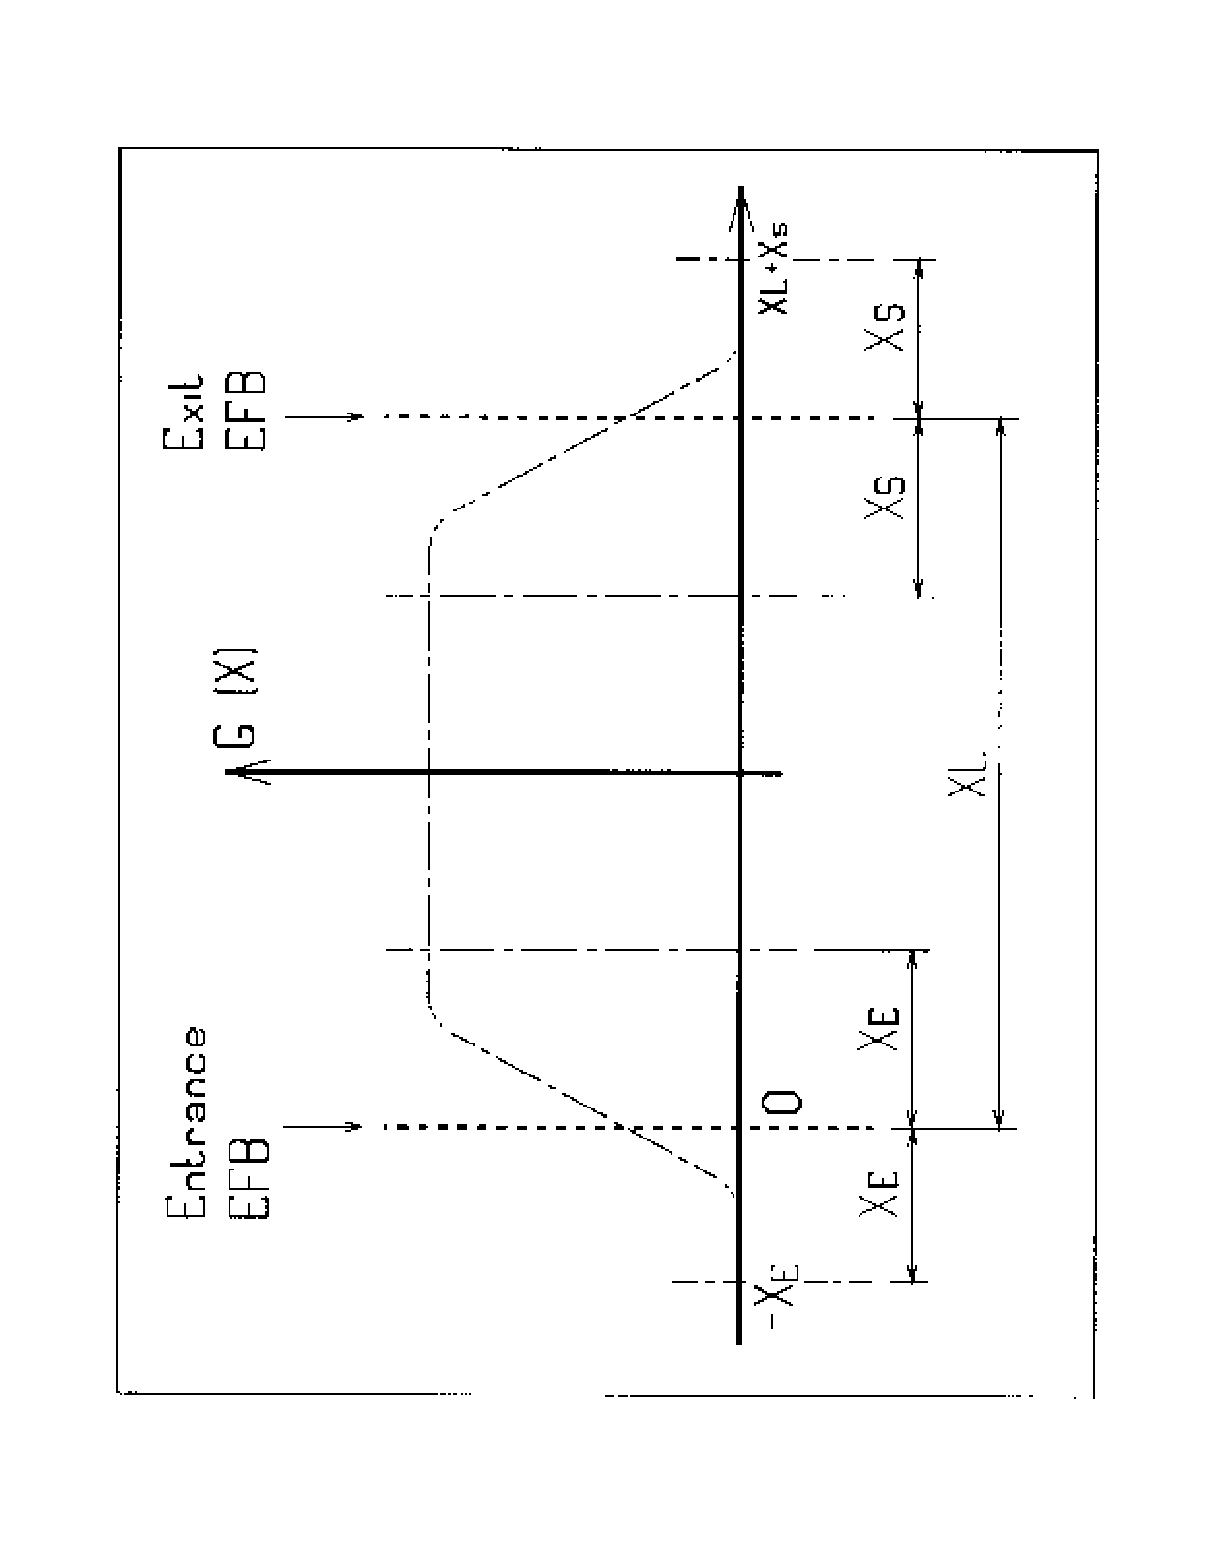
\includegraphics[height=10cm,angle=-90]{Fig27.ps}}
\hangcaption[Fig27]{\label{fig27}Scheme of the longitudinal field gradient $ G(X) $.\\
$ (OX) $ is the longitudinal axis of the reference frame $ (0,X,Y,Z) $ of \zgou.
The length of the element is $ \XL $.  Trajectories 
are ray-traced from $ -X_E $ to $ \XL+X_S $, by means of respectively prior and final 
automatic change of frame. 
}
\end{figure}



\newpage

\subsubsection*{SEPARA~: \SEPARATitl}\label{SEPARA} \index{SEPARA|textbf}
\medskip 

\noindent Note~: simulation by stepwise integration can be found in \textsl{WIENFILTER}.

\medskip

\textsl{SEPARA}  provides an analytic simulation of an electrostatic separator. 
Input data are the length $ L $ of the element, the electric field $ E $ and
the magnetic field $ B $. The mass $ m $ and charge $ q $ of the particles are
entered by means of the keyword \textsl{PARTICUL\index{PARTICUL}}.  
\medskip

\noindent The subroutines involved in \textsl{SEPARA} solve the following
system of three equations with three unknown variables $ S$, $Y$, $Z $ (while  $ X\equiv L $), that 
describe the cycloidal motion of a particle in $ \vec  E$,  $ \vec  B $ static
fields (Fig.~\ref{fig28}).   

\begin{align*}
	X &   =   -R  \cos \left( \dfrac{\omega S }{ \beta c} + \epsilon \right) 
	         -  \dfrac{\alpha S }{ \omega\beta c} + \dfrac{C_1 }{ \omega} \\
	Y &   =     R \sin  \left(\dfrac{\omega S }{ \beta c} + \epsilon \right) - 
	         \dfrac{\alpha }{ \omega^ 2} - \dfrac{C_2 }{ \omega}  + Y_0  \\
	Z &   =  S \sin (P_0)+Z_0   
\end{align*}
%
 where, $ S $ is the path length in the separator, $\alpha =-\dfrac{Ec^2 }{ \gamma}$ ,
   $   \omega =-\dfrac{Bc^2 }{m\gamma}$, $   C_1=\beta \sin (T_0) \cos (P_0) $ 
and $ C_2=\beta c  \cos (T_0) \cos (P_0) $ are initial conditions. 
$c$ = velocity of light, $ \beta c$ = velocity of the particle,  
$ \gamma =(1-\beta^ 2)^{-\dfrac{1 }{ 2}} $ 
and  $\tan \epsilon  =   (C_2+ \dfrac{\alpha}{\omega})/C_1 $.   $ Y_0$,   $ T_0$,  
$Z_0$,  $ P_0 $ are the initial 
coordinates of the particle in the \zgou\ reference  frame.  Here 
$\beta c $ and $\gamma$ are assumed constant, which is true as long as the change of momentum
due to the electric field remains negligible all along the separator.  
\medskip

\noindent The option index $\IA$ in the input data allows switching to inactive
element (thus equivalent to \textsl{ESL}), horizontal or vertical separator.  
Normally, $ E$,  $B $ and the value of $ \beta_W $ for wanted particles are related by 

$$ B(T) = - \dfrac{E\left(\dfrac{V }{ m}\right) }{ \beta_ W\cdot c\left(\dfrac{m }{ s}\right)} $$

 %\newpage
\vfill

%%%%%%%%%%%%%%figure%%%%%%%%%%%%%%
\begin{figure}[H]
%\vspace{20 truecm}
%%%Figure 28
\centerline{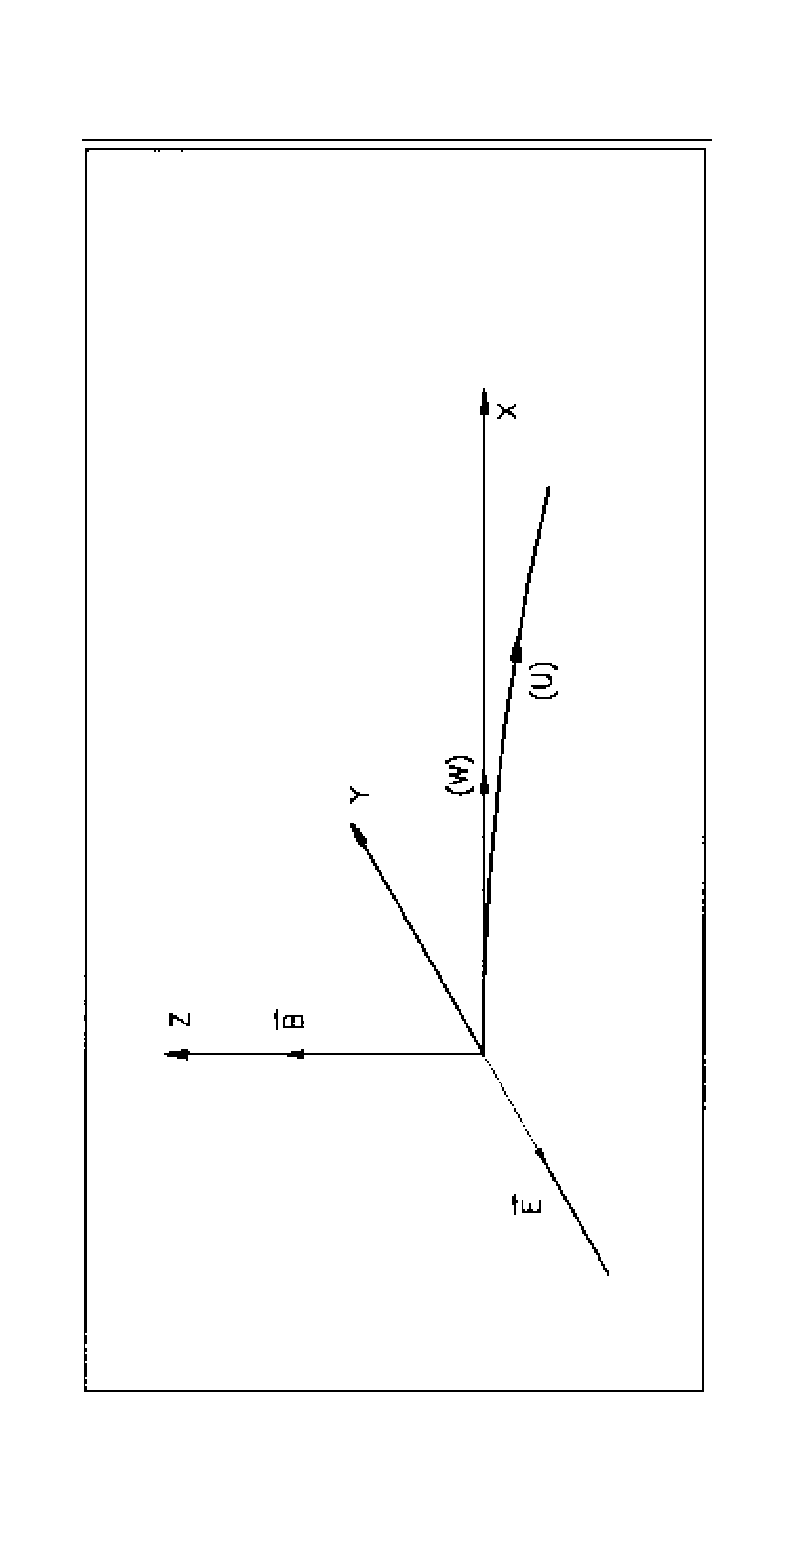
\includegraphics[height=15cm,angle=-90]{Fig28.ps}}
{\setlength{\captionwidth}{14cm}
\hangcaption[Fig28]{\label{fig28}Horizontal separation between a wanted particle, $ (W)$,  
and an unwanted particle, $ (U) $.  
$ (W) $ undergoes a linear motion while $ (U) $ undergoes a 
cycloidal motion.} }
\end{figure}
\vfill

\newpage

\subsubsection*{SEXTUPOL~: \SEXTUPOLTitl\ (Fig.~\protect\ref{fig29})} 
\medskip 
     \label{SEXTUPOL} \index{SEXTUPOL|textbf}  

The meaning of parameters for \textsl{SEXTUPOL} is the same as 
for \textsl{QUADRUPO\index{QUADRUPO}}.  
\medskip

\noindent In fringe field regions the magnetic field $ \vec  B(X,Y,Z) $ and
its derivatives up to fourth order are derived from the scalar potential approximated to 
7th order in $ Y $ and $ Z $

 \begin{align*}
 	V(X,Y,Z)    & =   \left(G- \dfrac{G^{\prime\prime} }{ 16}\, (Y^2+Z^2)+
	             \dfrac{G^{\quaprime} }{ 640}\, (Y^2+Z^2)^2\right) 
	             \left(Y^2Z-\dfrac{Z^3 }{ 3} \right)   \\
\text{with } ~ G_0 &   =  \dfrac{ B_0}{ R^2_0}
\end{align*}

\noindent The  modelling of the fringe field form factor  $G(X)$
 is described under \textsl{QUADRUPO}, p.~\pageref{QUADRUPO}. 

\medskip


\noindent Outside fringe field regions, or everywhere in sharp edge sextupole 
($ \lambda_E=\lambda_ S=0$),   $ \vec  B(X,Y,Z) $ in the magnet is given by 

\begin{align*}
	B_X &   =     0 \\
	B_Y &   =    2G_0YZ \\
	B_Z &   =     G_0(Y^2-Z^2)  
\end{align*}
\vfill

%%%%%%%%%%%%%%figure%%%%%%%%%%%%%%
\begin{figure}[H]
%\vspace{12 truecm}
%%%Figure 29
\centerline{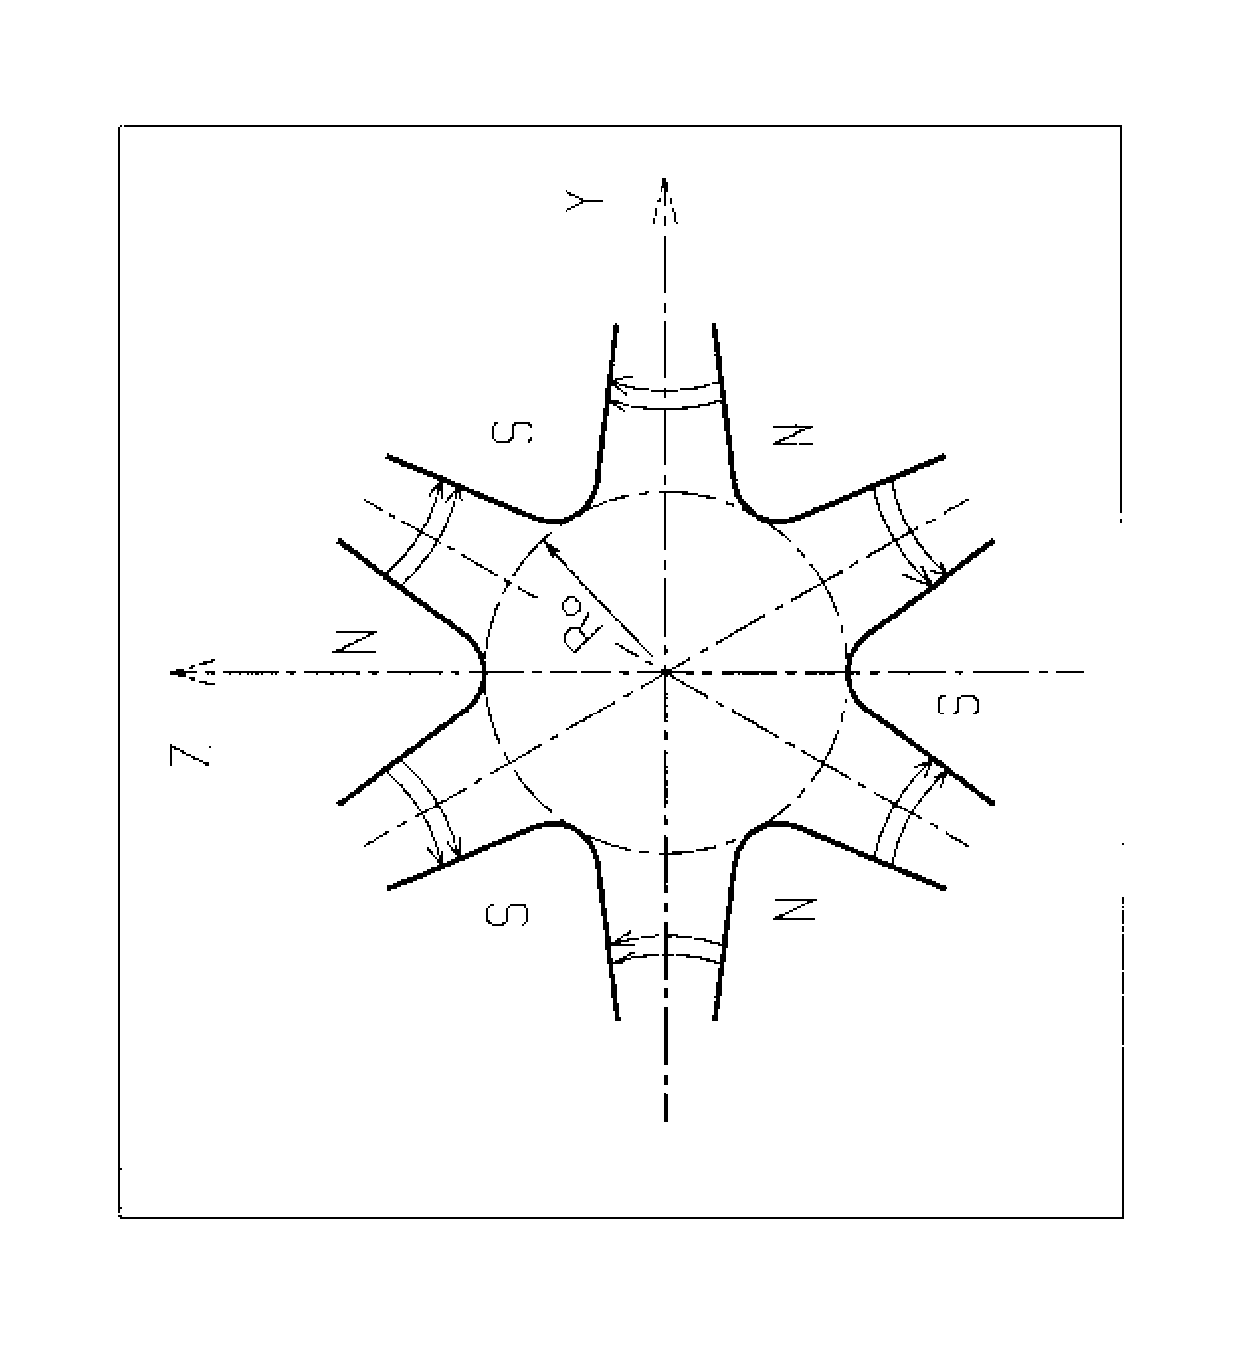
\includegraphics[height=12cm,angle=-90]{Fig29.ps}}
\caption{\label{fig29}Sextupole magnet}
\end{figure}
\vfill



\newpage

\subsubsection*{SOLENOID~: \SOLENOIDTitl\ (Fig.~\protect\ref{fig30}) } \label{SOLENOID} \index{SOLENOID|textbf} 
\medskip 

 The solenoidal magnet has an effective length $ \XL$,  a mean radius
$ R_0 $ and an asymptotic field  $ B_0=\mu_0 N I / \XL$ (\emph{i.e.}, $\int_{-\infty}^\infty 
B_X(X,r) dX = \mu_0 N I, ~\forall r<R_0$), wherein $B_X$=longitudinal field component, 
$ NI $  = number of Ampere-Turns, $\mu_0=4\pi  10^{-7} $. 
\medskip

\noindent The distance of ray-tracing beyond the effective length $ \XL$,   is 
$X_E $ at the entrance, and $ X_S $ at the exit (Fig.~\ref{fig30}).   
\medskip

\noindent Two methods are available for the computation of the field $ \vec  B(X,r)$ and its derivatives. 


\noindent Method~1~:   $ \vec  B(X,r)$, $r=(Y^2+Z^2)^{1/2} $ and its derivatives up to 
second order  at all $(X,Y,Z)$ are calculated following Ref.~\cite{Biblio17}, %%% [17]
based on the three complete elliptic integrals $K$, $E $ and $\Pi$. The latter 
are calculated with the algorithm proposed in the same reference, their
derivatives are calculated by means of recursive relations~\cite{Biblio18}.  %%[18] 

\medskip

\noindent This analytical model for the solenoidal field allows simulating an 
extended range of coil geometries (length, radius) 
provided that the coil thickness is small enough compared to the mean radius $ R_0 $. 
\medskip


\noindent In particular the field on-axis writes (taking $X=r=0$ at the center of the  solenoid) 
\begin{equation}
B_X(X,r=0) = \dfrac{\mu_0 N I }{2 \XL} \left[ \dfrac{\XL/2-X}{\sqrt{(\XL/2-X)^2}+R_0^2} 
+  \dfrac{\XL/2+X}{\sqrt{(\XL/2+X)^2}+R_0^2} \right]$$ 
 and yields the magnetic length 
$$L_{mag} \equiv  \dfrac{\int_{-\infty}^\infty B_X(X,r<R_0) dX }{B_X(X=r=0)} 
= \XL\sqrt{1+\dfrac{4R_0^2 }{\XL^2}} > \XL 
\label{EqSol}
\end{equation}
with in addition 
$$B_X(\textrm{center}) \equiv B_X(X=r=0) = 
      \dfrac{\mu_0 N I }{\XL\sqrt{1+\dfrac{4R_0^2}{\XL^2}}}.$$

\bigskip

\noindent Method~2~:  The second method available uses eq.~\ref{EqSol} above as a 1-D model and uses off-axis 
extrapolation to derive the field  and its derivatives at all $(X,Y,Z)$, following the method 
described in section~\ref{sec2.5.2}. 


\vfill

%%%%%%%%%%%%%%figure%%%%%%%%%%%%%%
\begin{figure}[H]
%\vspace{14 truecm}
%%%Figure 30
\centerline{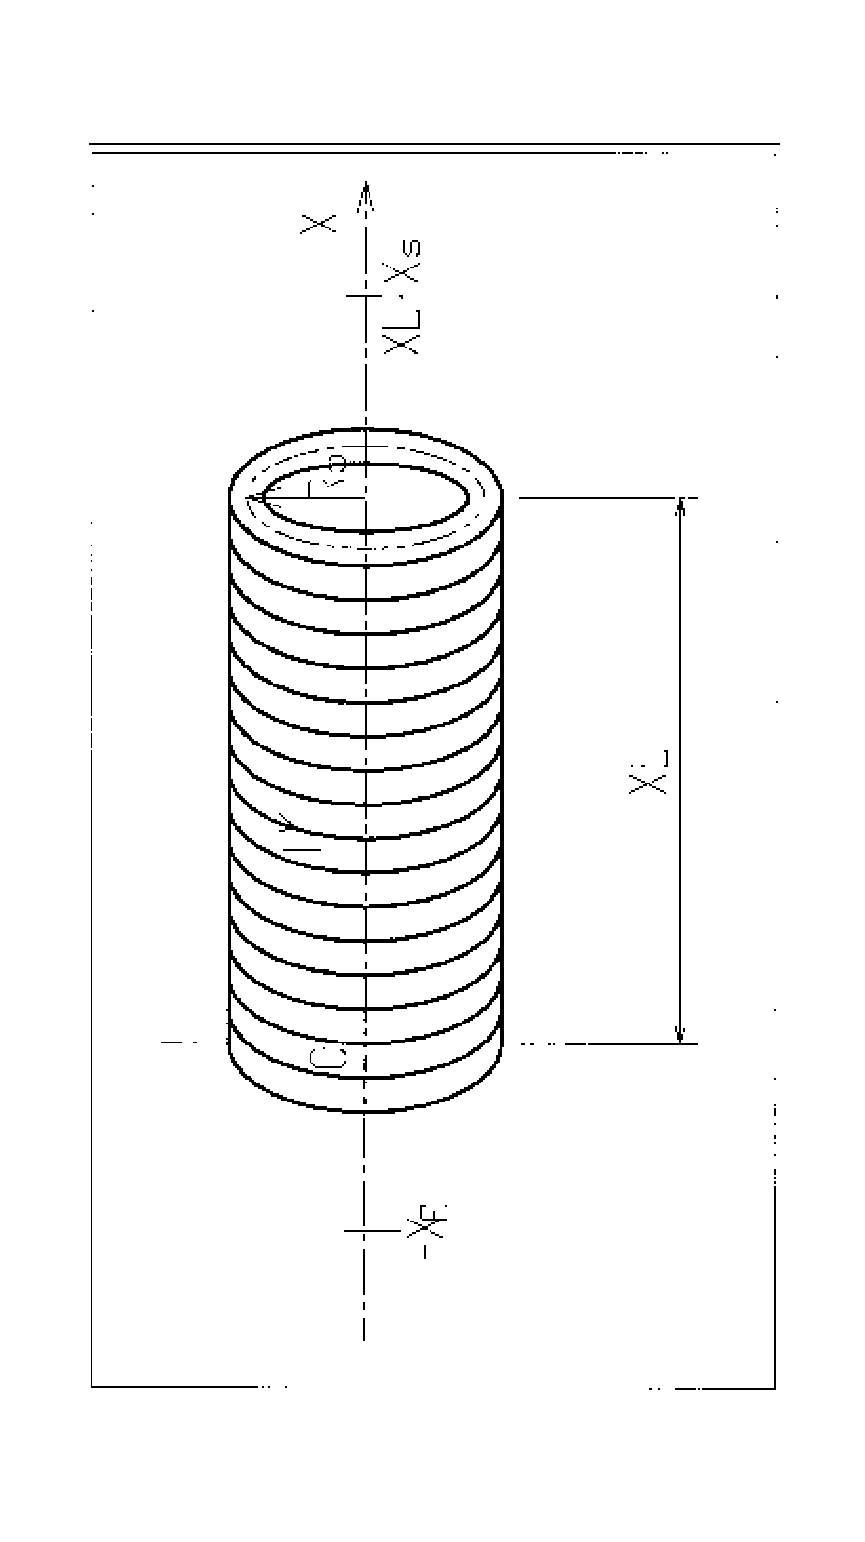
\includegraphics[height=15cm,angle=-90]{Fig30.ps}}
\caption{\label{fig30} Solenoidal magnet.}
\end{figure}
\vfill




\newpage

\subsubsection*{SPINR~: \SPINRTitl~\cite{SPINR}  } \label{SPINR} \index{SPINR|textbf} 
\medskip

\textsl{SPINR} causes spin precession, a local transformation on the spin vector of the particles, 
 as, \eg, in a local helical spin rotator.  Two options are 
available, as follows. 

\bigskip

\noindent \textbf{$\mathbf{IOPT  =  0}$} inhibits the keyword. 

\bigskip

\noindent \textbf{If $\mathbf{IOPT  =  1}$~:} the precession is defined by its axis, at angle  $\phi_Z$ with 
respect to \zgou's X-axis and assumed in the horizontal plane,  and by its value, $\mu$. 

\bigskip

\noindent \textbf{If $\mathbf{IOPT  =  2}$~:}  given the spin precession axis $\phi_Z$ - defined as  above -  
   the spin precession angle follows a function of the \textsl{reference} Lorentz factor~: 
  $$\mu (\gamma) = \left(\frac{B}{B_0}\right)^2 \times \left( C_0 + \frac{C_1}{\gamma} + \frac{C_2}{\gamma^2}  + \frac{C_3}{\gamma^3} \right) $$
 with $B$ and $B_0$ normally  a nominal and a reference magnetic field value, and $C_i$ empirical coefficients. 
The \textsl{reference} Lorentz factor corresponds to the reference rigidity 
 \BORO, as defined for instance with \textsl{[MC]OBJET}, possibly updated in the presence of acceleration 
(see section~\ref{sec4.6.RefBORO}, page~\pageref{sec4.6.RefBORO}). 

\newpage

\subsubsection*{TOSCA~: \TOSCATitl} \label{TOSCA} \index{TOSCA|textbf}
\medskip

 \textsl{TOSCA} is dedicated to the reading and treatment of 2-D or 
3-D Cartesian or cylindrical mesh field maps as  delivered by the
\textsl{TOSCA}  magnet computer code standard output.

\medskip

\noindent A pair of flags, \textsl{MOD}, \textsl{MOD2}, determine whether Cartesian or Z-axis cylindrical mesh is used, 
and the nature of the field map data set.

\medskip

\noindent The total number of field data files to be read is determined by the \textsl{MOD} flag 
(see below) and by the parameter $IZ$ that appears in the data list following the keyword. 
Each of these files contains the field components $B_X$, $B_Y$, $B_Z$ on an 
\mbox{($X$, $Y$)} mesh. $IZ = 1$ for a 2-D~map, and 
in this case $B_X$ and $B_Y$ are assumed  zero all over the map\footnote{Use 
\textsl{MAP2D}\index{MAP2D} in case non-zero $B_X$, $B_Y$ are to be taken into account in a 2-D map.}. 
For a 3-D~map with mid-plane symmetry, described with a set of 2-D maps at various $Z$, 
then  \textsl{MOD=0} and  $IZ\ge 2$, and thus, the first 
data file whose name follows in the data list is supposed to contain the median 
plane field (assuming $ Z=0 $ and  $ B_X=B_Y=0$), while the remaining  $IZ-1$ 
file(s) contain the $IZ-1$ additional  planes in increasing $Z$ order. For arbitrary 3-D~maps, 
 no  symmetry assumed, then  \textsl{MOD=1} and  
 the total number of maps (whose names follow in the data list) 
is $IZ$, such that  map number $[IZ/2]+1$ is the $Z = 0$ elevation one.

\medskip

\noindent The field map data file has to be be filled with a 
format that fits the  \FORTRAN\ reading sequence. 
The following is an instance, details and possible updates are to be found in the source  
file \texttt{'fmapw.f'}~:  

{\footnotesize
\begin{verbatim}
	   DO  1  K = 1, KZ
	     OPEN (UNIT = NL, FILE = FNAME, STATUS = `OLD' [,FORM='UNFORMATTED'])
	     DO  1  J = 1,  JY  
	       DO  1 I = 1, IX
                 IF (BINARY) THEN
                   READ(NL) Y(J), Z(K), X(I), BY(J,K,I), BZ(J,K,I), BX(J,K,I)
                 ELSE
	           READ(NL,100) Y(J), Z(K), X(I), BY(J,K,I), BZ(J,K,I), BX(J,K,I)
    100	           FORMAT(1X,6E11.2)
                 ENDIF
     1     CONTINUE
\end{verbatim}}
\medskip

\noindent $IX$ ($JY$, $KZ$)  is   the number of longitudinal 
(transverse horizontal, vertical) nodes of the 3-D uniform mesh. For letting \zgou\ know that these are binary files, 
FNAME must begin with  \mbox{`B\_'} or  \mbox{`b\_'}.  

\medskip


\noindent In addition to the \textsl{MOD=1, 2} cases above, one can have \textsl{MOD=12} and in that case a single file 
contains the all 3-D field map. 
See  table below and the \FORTRAN\  subroutine \texttt{fmapw.f} and its entries FMAPR, FMAPR2, for more details, in particular 
the  formatting of the field map data file(s). 

\medskip

\begin{center}
\renewcommand{\arraystretch}{1}
\begin{tabular}{llll}
\bf         MOD   &\bf      MOD2 &   & \\[1ex]
 \multicolumn{3}{l}{\underline{MOD $\leq$ 19 :    Cartesian mesh}}    \\[1.5ex]
 0 and $IZ=1$ &     none                &  \multirow{2}{80mm}{2-D map, a single  data file for  $B_Z(X,Y)|_{Z=0}$, mid-plane symmetry.} \\[4ex]
0  and $IZ>1$ &     none                &  \multirow{2}{80mm}{3-D map, 1+IZ/2 data files of upper half of magnet, one per (X,Y)$|_{0\leq Z\leq Z_{max}}$ plane, mid-plane symmetry.} \\[6ex]
        0     &    1, 2, 3              &  As previous case, just  different reading formats. \\[1ex]
        1     &  none                   &  \multirow{2}{80mm}{2- or 3-D map, IZ data files, one per (X,Y) plane, no symmetry assumed.} \\[3ex]
        1     &    1, 2, 3              &  As previous case, just  different reading formats. \\[1ex]
        3     &     none, 1             &  \multirow{3}{80mm}{AGS main magnet field map, 2-D, mid-plane symmetry assumed. MOD2=1 causes field to be perturbed by $(1+n_1\,dY+n_2\, dY^2+n_3\, dY^3)$ factor.} \\[9ex]
        12    &           none          &  \multirow{2}{80mm}{3-D map, single file, upper half of magnet, symmetry with respect to (X,Y)  mid-plane.} \\[4ex]
        12    &              1          &  \multirow{2}{80mm}{3-D map, single file, whole magnet volume (thus no symmetry assumed).}  \\[4ex]
        12    &              2          &  \multirow{2}{80mm}{3-D map, single file, 1/8th of the magnet,  symmetry wrt. (X,Y), (X,Z), (Y,Z) planes.}  \\[4ex]
        15    &              1-6        &  \multirow{2}{80mm}{3-D map, whole magnet volume (thus no symmetry assumed), up to 6 maps 
 summed up~: at all node, $\vec B = \sum_{i=1}^{i=MOD2} a_i \, \vec B_i $.}  \\[5ex]
 \multicolumn{2}{l}{\underline{MOD $\geq$ 20   : Cylindrical mesh}}   \\[1.5ex]
       20, 21  &                        &  \multirow{2}{80mm}{3-D map, single file, half a magnet, cyl. symmetry with respect to (Y,Z) plane.} \\[4ex]
       22, 24  &                        &  \multirow{2}{80mm}{3-D map, single file, half a magnet, symmetry with respect to (X,Y)  mid-plane.} \\[4ex]
%       25      &                        &  \multirow{2}{80mm}{2-D mid-plane field map, single file, full magnet, symmetry with respect to mid-plane} \\[3ex]
\end{tabular}
\end{center}

\medskip


\noindent The field $ \vec  B=(B_X,B_Y,B_Z) $ is normalized by means of 
\textsl{BNORM} in a similar way as in \textsl{CARTEMES\index{CARTEMES}}.  
 As well the  coordinates  X and Y (and Z in the case of a 3-D field map) are normalized by  the
  \textsl{X-[, Y-, Z-]NORM} coefficient (useful to convert to centimeters, the working units in  \zgoubi). 

\medskip

\noindent At each step of the trajectory of a particle inside the map, the
field and its derivatives are calculated 

 - in the case of 2-D map,  by means of a second or fourth order polynomial interpolation, 
depending on \textsl{IORDRE\index{IORDRE}} (\textsl{IORDRE} = 2, 25 or 4), as for 
\textsl{CARTEMES\index{CARTEMES}}, 

 - in the case of 3-D map, by means of a second order polynomial interpolation with a 
$3  \times   3   \times   3$-point parallelepipedic grid, as described in 
section~\ref{sec2.4.4}. 
\medskip

\noindent Entrance and/or exit integration boundaries between which the trajectories
are integrated in the field may be defined, in the same way as in  \textsl{CARTEMES\index{CARTEMES}}. 





\newpage

\subsubsection*{TRANSMAT~:  \TRANSMATTitl}\label{TRANSMAT}\index{TRANSMAT|textbf}
\medskip

\textsl{TRANSMAT} performs a second order transport of the particle coordinates 
in the following way 

$$ X_i = \sum_j R_{ij}X^0_j + \sum_{j,k} T_{ijk}X^0_jX^0_k $$
%
 where, $ X_i $ stands for any of the current coordinates $ Y$, $T$, $Z$, $P $, path length and 
momentum dispersion, and $ X^0_i $ stands for any of the initial coordinates.
$[R_{ij}]$ ($[T_{ijk}]$) is the first order (second order) 
transfer matrix as usually involved in second order beam optics~\cite{Biblio10}.      %%% [10]  
Second order transfer is optional.  The length of the element represented by 
the matrix may be introduced for the purpose of path length updating.  

\bigskip

\noindent Note~: \textsl{MATRIX\index{MATRIX}} delivers $[R_{ij}]$ and $[T_{ijk}]$ matrices in a format 
suitable for straightforward use with \textsl{TRANSMAT}.




\newpage

\subsubsection*{TRAROT~: \TRAROTTitl} \label{TRAROT} \index{TRAROT|textbf}
\medskip


UNDER DEVELOPMENT. Check before use. 

~

\noindent  This procedure transports particles into a new frame by translation and rotation. Effect on spin tracking\index{spin tracking}, 
particle decay and gas-scattering are taken into account (but not on synchrotron radiation).





\newpage


\subsubsection*{UNDULATOR~: \UNDULATORTitl}\label{UNDULATOR}  \index{UNDULATOR|textbf}

\medskip


\textsl{UNDULATOR} magnet. UNDER DEVELOPMENT. 



\newpage

\subsubsection*{UNIPOT~: \UNIPOTTitl} \label{UNIPOT} \index{UNIPOT|textbf}
\medskip 

The lens is cylindrically symmetric about the $ X$-axis.  
\medskip

\noindent The length of the first (resp. second, third) electrode is $ X1 $
(resp. $ X2$, $X3$). The distance between the electrodes is $ D$.  
The potentials are $ V1 $ and $V2$.  The inner radius is $ R_0 $ (Fig.~\ref{fig31}).  
The model for the electrostatic potential along the axis is~\cite{Biblio19}  %% [19]

$$ V(x) = 
    \dfrac{V2-V1 }{ 2\omega D} \left[
    \ln\, \dfrac{\cosh 
    	\dfrac{\omega \left(x+ \dfrac{X2}{ 2}+D \right) }{ R_0} }{
       \cosh \dfrac{\omega \left(x+\dfrac{X2 }{ 2}\right) }{ R_0}}  
    + \ln\,  \dfrac{\cosh \dfrac{\omega \left(x-\dfrac{X2 }{ 2}-D\right) }{R_0} }{
       \cosh \dfrac{\omega \left(x-\dfrac{X2 }{ 2}\right) }{R_0} }
     \right] $$
%
($ x  = $ distance from the center of the central electrode~;
$\omega$  = 1,318~; cosh = hyperbolic cosine), from which the field $ \vec  E(X,Y,Z) $ and its
derivatives are deduced following the procedure described in section~\ref{sec2.5.2}. 

\medskip

\noindent Use \textsl{PARTICUL\index{PARTICUL}} prior to \textsl{UNIPOT}, for the
 definition of particle mass and charge.

\medskip

\noindent The total length of the lens is $X1+X2+X3+2\,D$~; stepwise integration starts 
at entrance of the first electrode and terminates at exit of the third one. 

\vfill

%%%%%%%%%%%%%%figure%%%%%%%%%%%%%%
\begin{figure}[H]
%\vspace{14 truecm}
%%%Figure 31
\centerline{\includegraphics[height=15cm,angle=-90]{Fig31.ps}}
\caption{\label{fig31}Three-electrode cylindrical unipotential lens.}
\end{figure}
\vfill

\newpage

\subsubsection*{VENUS~: \VENUSTitl}  \label{VENUS}
\medskip 
\index{VENUS} 

\textsl{VENUS} is dedicated to a `rough' simulation
of SATURNE Laboratory's  \textsl{VENUS} 
dipole.  The field $ B_0 $ is constant inside the magnet, with longitudinal 
extent $ \XL $ and transverse extent $ \pm YL $~;  outside these limits, $ B_0=0$ 
(Fig.~\ref{fig32}).  

\vfill
%%%%%%%%%%%%%%figure%%%%%%%%%%%%%%
\begin{figure}[H]
%\vspace{18 truecm}
%%%Figure 32
\centerline{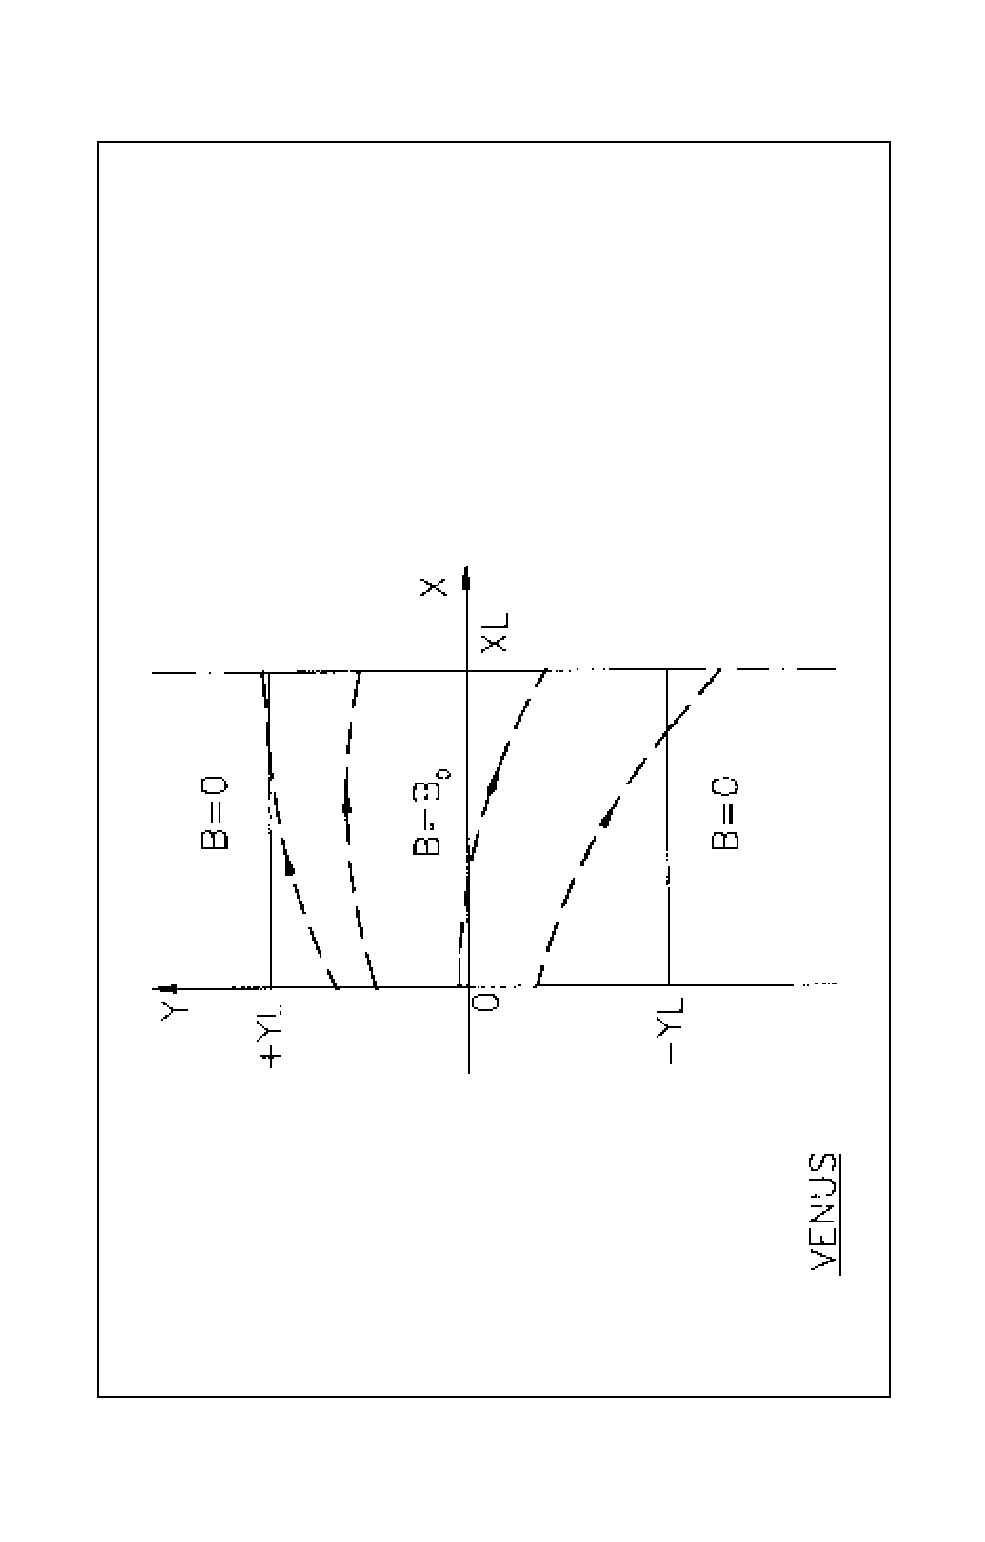
\includegraphics[height=15cm,angle=-90]{Fig32.ps}}
\caption{\label{fig32}Scheme of \textsl{VENUS} rectangular dipole.}
\end{figure}
\vfill

\newpage

\subsubsection*{WIENFILT~: \WIENFILTTitl}\label{WIENFILT} \index{WIENFILT|textbf}
\medskip 

\textsl{WIENFILT} simulates a Wien filter, with transverse and
orthogonal electric and magnetic fields $ \vec  E_Y$,  $ \vec  B_Z $ or $ \vec  E_Z$, 
 $ \vec  B_Y$ (Fig.~\ref{fig28}).
 It must be preceded by \textsl{PARTICUL\index{PARTICUL}} for the definition of particle mass and charge.  
\medskip

\noindent The length $ \XL $ of the element is the distance between its
entrance and exit EFB's. The electric and magnetic field intensities $ E_0 $ and $ B_0 $ in the 
central, uniform field region, normally satisfy the relation
 
 $$ B_0= - \dfrac{E_0 }{ \beta_ Wc} $$
%
 for the selection of `` wanted''  particles of velocity $\beta_Wc $. Ray-tracing in 
field fall-off regions extends over a distance $ X_E $ $ (X_S) $ beyond the
entrance (exit) EFB by means of prior and further automatic change of frame. Four sets
of coefficients $\lambda$, $ C_0-C_5 $ allow the description of the entrance and exit fringe 
fields outside the uniform field region, following the model~\cite{Biblio12} %% [12]

\begin{gather*}
	F = \dfrac{1 }{ 1+ \exp(P(s))} \\
	\intertext{where $  P(s) $ is of the term}
	    P(s) = C_0
	       +C_1 \left(  \dfrac{s }{ \lambda} \right) 
	       +C_2 \left( \dfrac{s }{ \lambda} \right)^2 
	       + C_3 \left( \dfrac{s }{ \lambda} \right)^3 
	       +C_4 \left( \dfrac{s }{ \lambda} \right)^4 
	       + C_5 \left(\dfrac{s }{ \lambda} \right)^5 
\end{gather*}
%
and $ s $ is the distance to the EFB.  When fringe fields overlap
inside the element (\emph{i.e.}, $ \XL\leq X_E+X_S$),  the field fall-off is expressed as

$$ F = F_E + F_S -1 $$
%
 where $ F_E(F_S) $ is the value of the coefficient respective to the entrance (exit) EFB. 
 
\noindent If $ \lambda_ E=0 $  ($\lambda_ S=0$)  for either the electric or
magnetic component, then both are considered as sharp edge fields and $ X_E(X_S) $ is forced 
to zero (for the purpose of saving computing time).  In this case, the magnetic wedge angle vertical first order focusing effect is simulated at entrance and exit by a kick $P_2 = P_1 - Z_1 \tan (\epsilon / \rho)$ applied to each particle ($P_1$, $P_2$ are the vertical angles upstream and downstream the EFB, $Z_1$ the vertical particle position at the EFB, $\rho$ the local horizontal bending radius and $\epsilon$ the wedge angle experienced by the particle~; $\epsilon$ depends on the horizontal angle T). This is not done for the electric field, however it is advised not to use a sharp edge electric dipole model since this entails non symplectic mapping, and in particular precludes accounting for momentum effects of the non zero longitudinal electric field component.

\newpage

\subsubsection*{YMY~: \YMYTitl} \label{YMY} \index{YMY|textbf}
\medskip 

\textsl{YMY}  performs a 180$^\circ$ rotation of particle coordinates with respect to the 
$ X $-axis, as shown  in Fig.~\ref{fig33}. 
This is done by means of a change of sign of $ Y $ and $ Z $ axes,  
and therefore coordinates, as follows 

$$ Y2=-Y1,\quad T2=-T1,\quad Z2=-Z1 \quad \text{and} \quad P2=-P1 $$

\vfill
%%%%%%%%%%%%%%figure%%%%%%%%%%%%%%
\begin{figure}[H]
%\vspace{18 truecm}
%%%Figure 33
\centerline{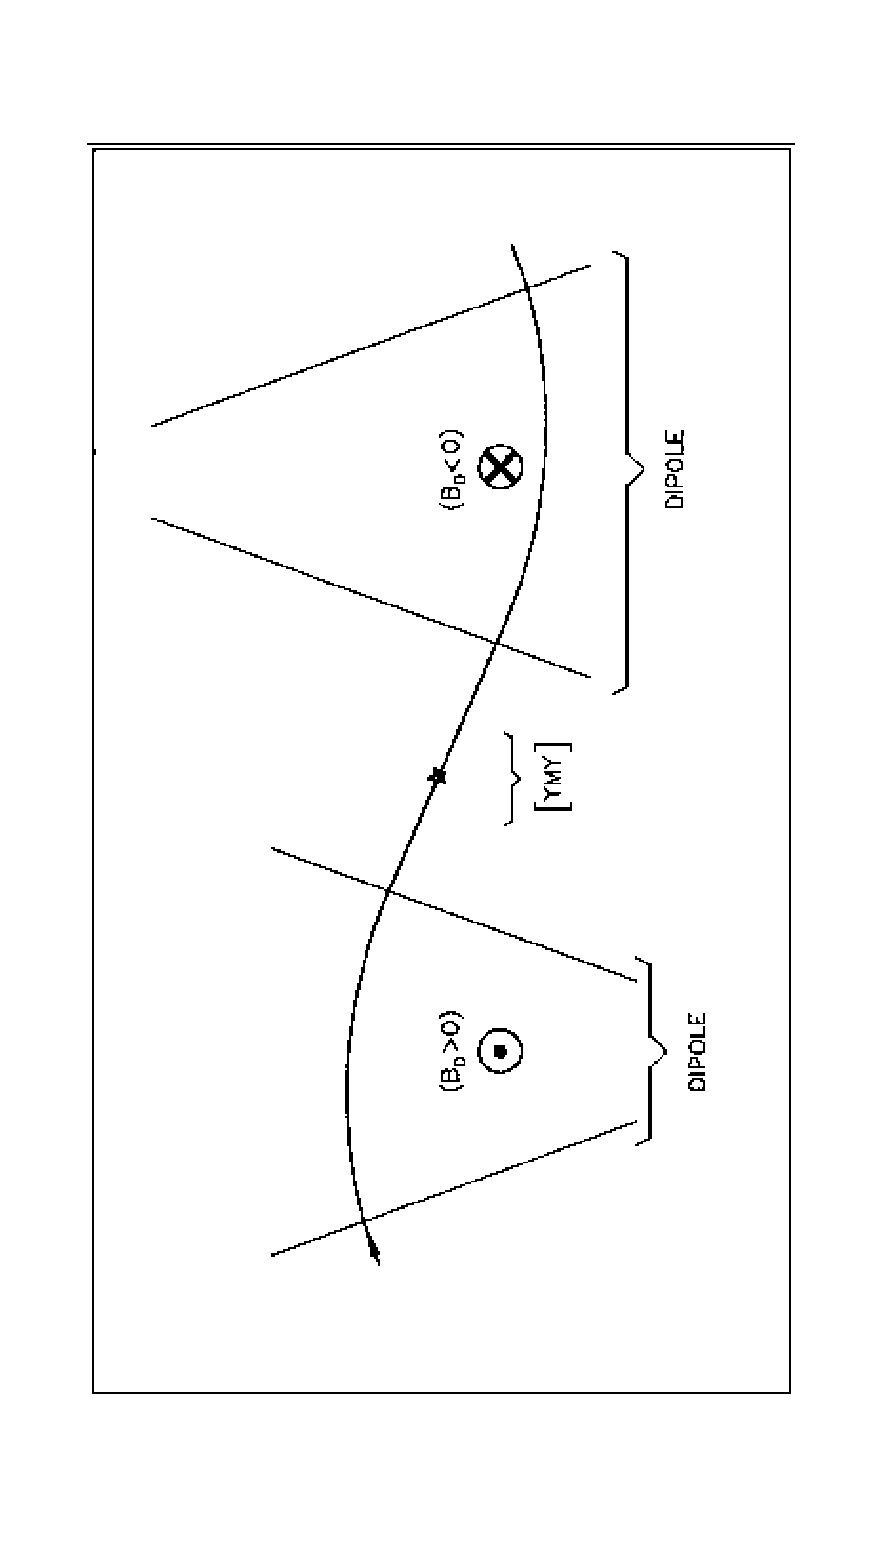
\includegraphics[height=15cm,angle=-90]{Fig33.ps}}
\caption{\label{fig33}\mbox{The use of $ YMY $ in a sequence of two identical
dipoles of opposite signs.}}
\end{figure}
\vfill






\newpage  %%%%% 

\subsection{Output Procedures} \label{sec4.5}

 These procedures are dedicated to the storage or printing of particle coordinates, 
histograms, spin coordinates\index{spin tracking}, etc. They may be called for at any spot in the data pile. 





\newpage

\subsubsection*{FAISCEAU, FAISCNL, FAISTORE~:  Print/Store particle coordinates} \label{FAISCEAU}\label{FAISCNL}
 \label{FAISTORE}\index{FAISCEAU|textbf} \index{FAISCNL|textbf}\index{FAISTORE|textbf}

\medskip 


$\bullet$ \textsl{FAISCEAU}  can be introduced anywhere in a structure 
data list (zgoubi.dat).  It produces a print  (into zgoubi.res) 
of  initial and actual coordinates of the  \IMAX\index{IMAX@{\IMAX}} particles at the location where it stands, 
together  tagging indices and letters, etc.  \index{tag, tag character} 

\medskip

\noindent $\bullet$  \textsl{FAISCNL} produces a lot more information on particles at current location, including 
spin components, decay distance, mass, charge, etc. (see list below), and stores it in a 
dedicated file \textsl{FNAME} (advised name is \textsl{FNAME} = `zgoubi.fai'  
(formatted write) or `b\_zgoubi.fai' (binary write) \index{zgoubi.fai}
if post-processing with \textbf{zpop}\index{zpop} should follow).  This file may further on be read by means of  \textsl{OBJET}, 
option \mbox{\KOBJ= 3}, or used for other purposes such as graphics (see Part~D of the Guide).  

\noindent The data written to that file are formatted and  ordered according to the \FORTRAN\ sequence 
in the subroutine \texttt{impfai.f}, where details and possible updates are to found. 
The following is an instance~: 

{\footnotesize
\begin{verbatim}
    OPEN (UNIT = NL, FILE = FNAME, STATUS = `NEW')
      IF(BINARY) THEN
        DO 2 I=1,IMAX
            P = BORO*CL9 *F(1,I) * AMQ(2,I)
            ENERG = SQRT(P*P + AMQ(1,I)*AMQ(1,I))
            ENEKI = ENERG - AMQ(1,I)
            WRITE(NFAI)
     1      IEX(I),-1.D0+FO(1,I),(FO(J,I),J=2,MXJ),                 tag, initial D-1,Y,T,Z,P,S,Time
     2      -1.D0+F(1,I),F(2,I),F(3,I),(F(J,I),J=4,MXJ),            current D_i,Y,T,Z,P,S,Time
     >      (SI(J,I),J=1,4),(SF(J,I),J=1,4),                        spin components, initial and current
     >      ENEKI,ENERG,                                            energy
     4      I,IREP(I), SORT(I),(AMQ(J,I),J=1,5),RET(I),DPR(I),PS,   particle#,loss S,mass,Q,G,life time
     5      BORO, IPASS, NOEL, KLEY,LBL1,LBL2,LET(I)                BORO, pass#,element#,keyword,labels
 2      CONTINUE
      ELSE
        DO 1 I=1,IMAX
          P = BORO*CL9 *F(1,I) * AMQ(2,I)
          ENERG = SQRT(P*P + AMQ(1,I)*AMQ(1,I))
          ENEKI = ENERG - AMQ(1,I)
          WRITE(NFAI,110)
     1    IEX(I),-1.D0+FO(1,I),(FO(J,I),J=2,MXJ),
     2    -1.D0+F(1,I),F(2,I),F(3,I),
     3    (F(J,I),J=4,MXJ),
     4    (SI(J,I),J=1,4),(SF(J,I),J=1,4),
     5    ENEKI,ENERG,
     6    I,IREP(I), SORT(I),(AMQ(J,I),J=1,5),RET(I),DPR(I),PS,
     7    BORO, IPASS, NOEL, 
     8    TX1,KLEY,TX1,TX1,LBL1,TX1,TX1,LBL2,TX1,TX1,LET(I),TX1
          INCLUDE "FRMFAI.H"
 1      CONTINUE
      ENDIF

 110     FORMAT(1X,

C1               KEX,      XXXO,(FO(J,IT),J=2,MXJ)
     >  1P,      1X,I2,    7(1X,E16.8)

C2              XXX,Y,T*1.D3,
     >         ,3(1X,E24.16)

C3       Z,P*1.D3,SAR,TAR 
     >   ,4(1X,E24.16)

C4       SXo, SYo, SZo, So, SX, SY, SZ, S
     >   ,8(1X,E15.7)

C5        ENEKI,ENERG
     >   ,2(1X,E16.8)

C6       IT,IREP(IT),   SORT(IT), (AMQ(J,I),J=1,5), RET(IT), DPR(IT), PS
     >   ,2(1X,I6),   9(1X,E16.8)

C7         BORO,   IPASS, NOEL,    
     >   ,1X,E16.8,  2(1X,I6)

C8            'KLEY',    ('LABEL(NOEL,I)',I=1,2),           'LET(IT)'
     >    ,1X,A1,A10,A1,   2(1X,A1,A ,A1),                   1X,3A1)
\end{verbatim}}
\medskip

\noindent The meaning of the main data is the following (see the keyword \textsl{OBJET})
\medskip

{\renewcommand{\arraystretch}{1}
 \begin{tabular}{>{\sl}l!{~:}l}
	$LET(I) $  & one-character string, for tagging particle number $I$  \\  \index{tag, tag character} 
	$\IEX\index{IEX@{\IEX}}$, $I$, $IREP(I)$   &  flag, particle number, index  \\
	 $FO(1-6, I)$  &  coordinates $D$, $Y$, $T$, $Z$, $P$ and path
	                 length at the origin of the structure\\
	 $F(1-6, I)$  &  \id\, at the current position\\
     $SORT(I)$ & path length at which the particle has possibly been stopped\index{stopped particles}\\
      \multicolumn{1}{c}{  }       & (see \textsl{CHAMBR} or \textsl{COLLIMA})\\
     $RET(I)$, $DPR(I)$ & synchrotron phase space coordinates~; \textsl{RET} =phase (radian),\\
      \multicolumn{1}{c}{  }     &   \textsl{DPR} = momentum dispersion (MeV/c) (see \textsl{CAVITE}) \\
    \textsl{IPASS}  &  turn number (see \textsl{REBELOTE\index{REBELOTE}}) \\
 etc.
     \end{tabular}}
\medskip

\noindent $\bullet$  \textsl{FAISTORE} has an effect similar to \textsl{FAISCNL}, with two more features. 

- On the first data line, \textsl{FNAME} may be followed 
by a series of up to 10 \LABEL's\index{LABEL@{\LABEL}}.     If there is no 
label, the print occurs by default at the location of \textsl{FAISTORE}~; if there are labels the 
print occurs right downstream of all optical elements wearing those labels
 (and no longer at the \textsl{FAISTORE} location). 

- The next data line 
gives a parameter, $IP$~: printing will occur at pass 1 and then at every $IP$ other pass, if 
using \REBELOTE\index{REBELOTE} with \textsl{NPASS}\index{NPASS} $ \geq IP-1$. 

\medskip

\noindent For instance the following data input in zgoubi.dat~: 

\medskip

{\renewcommand{\arraystretch}{1}
\begin{tabular}{lll}
	\textsl{FAISTORE} &  &   \\
	zgoubi.fai \index{zgoubi.fai} & \textsl{HPCKUP} & \textsl{VPCKUP}  \\
	12 &  & 
\end{tabular}}
\medskip

\noindent will result in output prints into zgoubi.fai, at pass 1 and then at every 12~other 
pass, each time elements of the zgoubi.dat \index{zgoubi.dat} data list labeled either \textsl{HPCKUP}
or \textsl{VPCKUP} are encountered.

\medskip

\noindent\underline{Note}
\medskip 

\noindent Binary storage can be obtained from \textsl{FAISCNL} and \textsl{FAISTORE}. This is for 
the sake of compactness and access speed, for instance  in case  voluminous amounts of 
data would have to be manipulated using \zpop. 

\medskip 
\noindent This is achieved by giving the storage file a name of the form \textsl{b\_FNAME} 
or \textsl{B\_FNAME}  (\emph{e.g.}, `b\_zgoubi.fai'). The \FORTRAN\ \textsl{WRITE} list 
is the same as in the \textsl{FORMATTED} case above.  

\medskip
\noindent This is compatible with the \textsl{READ} statements in \textbf{zpop} that will recognize binary storage 
from that very radical 'b\_' or 'B\_'. 



\newpage

\subsubsection*{FOCALE, IMAGE[S]~: Particle coordinates and beam size~;  localization and
size  of  horizontal waist}\label{FOCALE}\label{IMAGE}\label{IMAGES}
\index{FOCALE|textbf}\index{IMAGE|textbf}\index{IMAGES|textbf}
\medskip 

\textsl{FOCALE}  calculates the dimensions of the beam and its mean 
transverse position, at a longitudinal distance $ \XL $ from the position 
corresponding to the keyword \textsl{FOCALE}.  
\medskip

\noindent\textsl{IMAGE}  computes the location and size
of the closest horizontal waist.  
\medskip

\noindent\IMAGES\index{IMAGES}  has the same effect as \textsl{IMAGE\index{IMAGE}},
 but, in addition, for a 
non-monochromatic beam it calculates as many waists as there are distinct momenta in 
the beam, provided that the object has been defined with a classification of momenta 
(see \textsl{OBJET\index{OBJET}}, \KOBJ = 1, 2  for instance).  
\medskip

\noindent Optionally, for each of these three procedures, \zgou\ can
list a trace of the coordinates in the $ X$, $Y $ and in the $ Y$, $Z $ planes.  
\medskip

\noindent The following quantities are calculated for the $ N $ particles of
the beam (\textsl{IMAGE,   FOCALE}) or of each group    of momenta 
(\textsl{IMAGES\index{IMAGES}})  
\medskip

\begin{itemize}
\item[$\bullet$]Longitudinal position~: 
       \begin{align*}
       \text{\textsl{FOCALE}~:} & \quad  X=\XL  \\
       \text{\textsl{IMAGE[S]}~:} & \quad   X    = - 
    \dfrac{ \sum^ N_{i=1}Y_i\ast \text{tg} T_i- 
         \left( \sum^ N_{i=1}Y_i\ast \sum^N_{i=1}\text{tg} T_i \right)\, /N }{%
        \sum^ N_{i=1}\text{tg} ^2T_i- \left( \sum^ N_{i=1}\text{tg} T_i\right)^2\, /N} \\ 
            & Y   =   Y_1+X  \ast   \text{tg} T_1  
        \end{align*}    
where $ Y_1 $ and $ T_1 $ are the coordinates of the first particle
of the beam (\textsl{IMAGE, FOCALE}) or the first particle of each group of momenta 
(\textsl{IMAGES\index{IMAGES}}). 

\item[$\bullet$]Transverse position of the center of mass of the waist 
(\textsl{IMAGE[S]}) or of the beam (\textsl{FOCALE}), with respect to the reference trajectory 

$$ \YM = \dfrac{1 }{ N} \sum^ N_{i=1}(Y_i+X  \text{tg} T_i)-Y=
      \dfrac{1 }{ N} \sum^ N_{i=1}Y\, M_i $$

\item[$\bullet$]FWHM of the image (\textsl{IMAGE[S]}) or of the beam 
(\textsl{FOCALE}), and  total width, respectively, $ W $ and $ WT $

\begin{align*}
	W &   =     2.35 \left( \dfrac{1 }{ N} \sum^ N_{i=1}Y\ M^2_i - Y\ M^2 \right)^{\dfrac{1}{2}} \\ 
	WT &   =    \max (\YM_i)- \min  (\YM_i)  
\end{align*}
\end{itemize}



\newpage

\subsubsection*{FOCALEZ, IMAGE[S]Z~: Particle coordinates and beam size~;  localization and 
size  of  vertical waist}\label{FOCALEZ}\label{IMAGEZ}\label{IMAGESZ}
 \index{FOCALEZ|textbf}\index{IMAGEZ|textbf}\index{IMAGESZ|textbf} 
\medskip 
          
Similar to \textsl{FOCALE} and \textsl{IMAGE[S]}, but the calculations are performed 
with respect to the vertical coordinates $ Z_i $ and $ P_i $, in place of $Y_i $ 
and $ T_i$. 
\vfill

\newpage

\subsubsection*{HISTO~: \HISTOTitl}\label{HISTO} \index{HISTO|textbf}
\medskip

Any of the coordinates used in \zgou\ may be histogrammed,
namely initial  $ Y_0$,  $ T_0$,  $ Z_0$,  $ P_0, $ $ S_0 $, $ D_0 $  or current 
$ Y$, $T$, $Z$, $P$, $S$, $D$ particle coordinates ($ S=$ path length~;  
$ D $ may change  in decay process simulation with \textsl{MCDESINT\index{MCDESINT}}, 
or when ray-tracing in $ \vec  E $ fields), and also spin coordinates\index{spin tracking} and
modulus $ S_X$, $ S_Y$,  $ S_Z $ and $ \left\Vert\vec  S \right\Vert   $.  
\medskip

\noindent\textsl{HISTO\index{HISTO}}  can be used in conjunction with 
\textsl{MCDESINT\index{MCDESINT}}, for statistics 
on the decay process, by means of \textsl{TYP}.  \textsl{TYP} is a one-character string.  
If it is set equal to `S', only secondary particles (they are tagged with an 'S') will be   \index{tag, tag character} 
histogrammed.  If it is set equal to `P', then only  parent particles (non-'S') will be histogrammed.  
For no discrimination  between S-econdary and P-arent particles,  \textsl{TYP} = `Q'  must be
used.  
\medskip

\noindent The dimensions of the histogram (number of lines and columns) may be
modified. It can be normalized with \textsl{NORM} = 1, to avoid saturation.  
\medskip

\noindent Histograms are indexed with the parameter  $\NH$.  This allows making
independent histograms of the same coordinate at several locations 
in a structure.  This is also useful when piling up problems in a single input data 
file  (see also \textsl{RESET}). $\NH$ is in the range 1-5.  
\medskip

\noindent If \REBELOTE\index{REBELOTE} is used, the statistics on the $1+$\textsl{NPASS}\index{NPASS}
runs in the structure will add up. 



\newpage

\subsubsection*{IMAGE[S][Z]~: \IMAGESZTitl}
\medskip 

\noindent See FOCALE[Z]. 


\vfill



\newpage

\subsubsection*{MATRIX~: \MATRIXTitl}\label{MATRIX} \index{MATRIX|textbf}
\medskip

\textsl{MATRIX}  causes the calculation of the transfer coefficients through the optical 
structure, from the \textsl{OBJET} down to the location where \textsl{MATRIX}  is introduced in the structure, or, 
upon option, down to the horizontal focus closest to that location.  
In this last case the position of 
the focus is calculated automatically in the same way as the position of the 
waist in \textsl{IMAGE}. Depending on option \textsl{IFOC},  \textsl{MATRIX} also
delivers the beam matrix and betatron phase advances or (case of a periodic structure) periodic beam matrix and tunes, 
chromaticities\index{chromaticity@{chromaticity}|textbf}  and other global parameters. 



\medskip

\noindent Depending on the value of option \textsl{IORD}, different procedures follow   

\medskip

\begin{itemize}
\item[$\bullet$] If \textsl{IORD} = 0, \textsl{MATRIX}  is inhibited (equivalent to 
\textsl{FAISCEAU}, whatever \textsl{IFOC}). 

\item[$\bullet$] If \textsl{IORD} = 1, the first order transfer matrix 
$ [R_{ij}]$ is calculated, from a third order approximation of the coordinates. For instance 
$$  Y^+    =   \left( \dfrac{Y}{T_0} \right)\, T_0
	             + \left(\dfrac{Y }{ T^2_0} \right)\, T^2_0 
	             + \left(\dfrac{Y }{ T^3_0} \right)\, T^3_0,   ~ ~ ~ ~ ~ ~ 
	 Y^-    =    - \left(\dfrac{Y }{ T_0} \right)\, T_0 
	             + \left(\dfrac{Y }{ T^2_0} \right)\, T^2_0 -
	             \left(\dfrac{Y }{ T^3_0} \right)\ T^3_0 $$
\noindent will yield, neglecting third order terms, 
$$          R_{11} = \left(\dfrac{Y }{ T_0} \right) = \dfrac{Y^+-Y^- }{ 2T_0} $$

\smallskip 

In addition, if \textsl{OBJET}, \textsl{KOBJ} = 5.01 is used (hence introducing initial optical function values, 
$\alpha_{Y,Z}$, $\alpha_{Y,Z}$, $D_{Y,Z}$, $D'_{Y,Z}$), 
then, using the $R_{ij}$ above,  \textsl{MATRIX} will transport  the  optical functions and phase advances 
$\phi_Y$, $\phi_Z$, following

\begin{equation}
\left(
\begin{array}{c}
\beta \\
\alpha \\
\gamma \\
\end{array}
\right)_{at~\textsl{MATRIX}}
=
\left(
\begin{array}{ccc}
R_{11}^2      &  -2R_{11}R_{12} &  R_{12}^2 \\
-R_{11}R_{21} &  R_{12}R_{21} &  R_{11}R_{12} \\
R_{21}^2      &  -2R_{21}R_{22} &  R_{22}^2 \\
\end{array}
\right)
\left(
\begin{array}{c}
\beta \\
\alpha \\
\gamma \\
\end{array}
\right)_{at~\textsl{OBJET}}       \nonumber
\end{equation}

\begin{eqnarray}
\Delta \phi_Y =  A\!\tan \dfrac{R_{12}}{(R_{11}\beta_{Y,\textsl{objet}} - R_{12}\alpha_{Y,\textsl{objet}})}, ~ ~ \Delta \phi_Z =  A\!\tan\dfrac{R_{34}}{(R_{33}\beta_{Z,\textsl{objet}} - R_{34}\alpha_{Z,\textsl{objet}})} , \\[3ex]
~ ~ ~   \phi_{Y, Z} \rightarrow \phi_{Y,Z} + 2 \pi ~ ~ ~ 
\textrm{if} ~ \phi_{Y,Z} < 0, \textrm{given} ~ ~ [0,\pi] \textrm{ Atan determination}   \nonumber
\end{eqnarray}

\noindent and print these out. 

\item[$\bullet$] If \textsl{IORD} = 2, fifth order Taylor expansions are used for the 
calculation of the first order transfer matrix $ [R_{ij}] $ and of 
the second order matrix $[T_{ijk}]$.  Other higher order coefficients are also calculated. 
\end{itemize}

\medskip

\noindent An automatic generation of an appropriate object for the use of \textsl{MATRIX}  can be obtained 
using the procedure \textsl{OBJET}~(pages~\pageref{OBJET},~\pageref{OBJET-B}), as follows

\noindent - if  \textsl{IORD} = 1, use \textsl{OBJET}(KOBJ = 5[.NN, NN=01,99]), 
that generates up to 99*11 sets of initial coordinates. In this case, up to ninety nine matrices 
may be calculated, each one \wrt\ to the reference trajectory of concern. 

\noindent - if  \textsl{IORD} = 2, use \textsl{OBJET}(KOBJ = 6)  that generates 
  61~sets of initial coordinates. 


\medskip

\noindent The next option, \textsl{IFOC}, acts as follows \par

\begin{itemize}
\item[$\bullet$] If \textsl{IFOC} = 0,  the transfer coefficients are calculated
at the location of \textsl{MATRIX\index{MATRIX}}, and with respect to the reference trajectory. 
For instance, $ Y^+ $ and $ T^+ $ above are defined for particle number $ i $ as 
$Y^+=Y^+(i)-Y(Ref)$,  and $ T^+=T^+(i)-T(\textrm{ref.})$.  

\item[$\bullet$] If \textsl{IFOC} = 1, the transfer coefficients are calculated at the 
horizontal focus  closest to \textsl{MATRIX\index{MATRIX}} (determined 
automatically), while the reference direction is that of the reference  particle. For 
instance, $ Y^+ $ is defined for particle number $ i $ as $ Y^+=Y^+(i) -Y_{\text{focus}} $, 
while  $ T^+ $ is defined as $ T^+=T^+(i)-T(\textrm{ref.)}$).  

\item[$\bullet$] If \textsl{IFOC} = 2, no change of reference frame is 
performed~: the coordinates refer to the current frame. Namely, $ Y^+=Y^+(i)$, 
$ T^+=T^+(i)$,  etc. \

\paragraph{\large Periodic Structures} 

\item[$\bullet$] If \textsl{IFOC} = 10  +  \textsl{NPeriod}, then, 
from the 1-turn transport matrix as obtained in the way described above,
 \textsl{MATRIX\index{MATRIX}} calculates periodic parameters characteristic  of the structure 
such as  optical functions and tune numbers, assuming that it is \textsl{NPeriod}-periodic, 
and  in the coupled hypothesis, based on the Edwards-Teng method~\cite{Coupling}. \index{coupling|textbf}

If  \textsl{IORD} = 2 additional 
periodic parameters are computed such as chromaticities, \index{chromaticity@{chromaticity}} beta-function momentum dependence, 
 etc. 


\end{itemize}

 

\medskip

\noindent  Addition of ``\textsl{PRINT}'' following \textsl{IORD, IFOC [, coupled]} will cause 
stacking of \textsl{MATRIX} output data into   zgoubi.MATRIX.out \index{zgoubi.MATRIX.out|textbf} 
file (convenient for use with \emph{e.g.} gnuplot type of data treatment software). 

\medskip

\noindent  Addition of ``\textsl{coupled}'' next to \textsl{IORD, IFOC [, PRINT]}, in the case of 
periodic beam matrix request (i.e., \textsl{IFOC} = 10  +  \textsl{NPeriod}) will cause use of coupled formalism. 




\newpage

 
\subsubsection*{PICKUPS~: \PICKUPSTitl}\label{PICKUPS} \index{PICKUPS|textbf}
\medskip

\noindent \textsl{PICKUPS} computes the coordinates of the beam centroid, 
at one or more \LABEL'ed\index{LABEL@{\LABEL}} keyword(s). 
 These coordinates are the average values of the coordinates of the  particles in a bunch. 
That (list of) \LABEL(s) is specified by the user, as part of the arguments under the keyword  \textsl{PICKUPS}.

\medskip
\noindent In conjunction with \textsl{REBELOTE}\index{REBELOTE} in the case of a periodic structure, 
  \textsl{PICKUPS} thus effectively delivers the closed orbit coordinates.       \index{closed orbit} 

\medskip






\newpage


\subsubsection*{PLOTDATA~: \PLOTDATATitl~\protect\cite{BiblioPlot}} \label{PLOTDATA} \index{PLOTDATA|textbf}

\medskip

\noindent  \textsl{PLOTDATA} was at the origin implemented for the purpose of plotting particle 
coordinates using the TRIUMF PLOTDATA package. However nothing precludes using it 
with a different aim. 

\medskip

\noindent  The \textsl{PLOTDATA} keyword can be introduced at up to 20 locations in zgoubi.dat.  There, particle coordinates 
will be stored in a local array, \texttt{FF}. They are overwritten at each pass. Usage of \texttt{FF} is left to the user, 
see \FORTRAN\ subroutine \texttt{pltdat.f}. 


\newpage

\subsubsection*{SPNPRNL, SPNSTORE~: Print/Store spin coordinates}
       \label{SPNPRNL} \label{SPNSTORE}\index{SPNPRNL|textbf}\index{SPNSTORE|textbf}

\medskip 

\noindent  $\bullet$   \textsl{SPNPRNL} has similar effect to \textsl{SPNPRT} (page~\pageref{SPNPRT}), 
except that the information is
stored in a  dedicated file \textsl{FNAME} (should post-processing with \textbf{zpop}\index{zpop} follow, 
advised name is \textsl{FNAME} = `zgoubi.spn' (formatted write) or `b\_zgoubi.spn' (binary write) \index{zgoubi.spn}). 
The data are formatted and ordered according to the  \FORTRAN\ sequence found in the subroutine \texttt{spnprn.f}, 
with meaning of printed quantities as follows~: 

\medskip

 \begin{tabular}{>{\sl}l!{~:}l}
	 LET(I),IEX(I)\index{IEX@{\IEX}}  &  tagging character and flag (see \textsl{OBJET}) \\  \index{tag, tag character} 
	 SI(1-4,I) & spin components\index{spin tracking} $SX$, $SY$, $SZ$  and modulus, at the origin\\
	 SF(1-4,I)   &  \id\, at the current position\\
	  GAMMA &   Lorentz relativistic factor\\
	  I  &  particle number\\
	 IMAX &  total number of particles ray-traced (see  \textsl{OBJET})\\
	 IPASS &  turn number (see \textsl{REBELOTE})\\
 \end{tabular}

\medskip

\noindent  $\bullet$   \textsl{SPNSTORE} has an effect similar to \textsl{SPNPRNL}, with two more features. 

- On the first data line, \textsl{FNAME} may be followed 
by a series of up to 10 \LABEL's\index{LABEL@{\LABEL}} proper to the elements of the zgoubi.dat data 
file at the exit of which the print should occur~; if no label is given, 
the print occurs by default at the very location of \textsl{SPNSTORE}~; 
if  labels are given, then print occurs right downstream of all optical elements wearing those labels
 (and no longer at the \textsl{SPNSTORE} location). 

- The next data line 
gives a parameter, $IP$~: printing will occur every $IP$ other pass, when 
using \REBELOTE\index{REBELOTE} with \textsl{NPASS}\index{NPASS} $ \geq IP-1$. 

For instance the following data input in zgoubi.dat~: 

\medskip

{\renewcommand{\arraystretch}{1}
\begin{tabular}{lll}
	\textsl{SPNSTORE} &  &   \\
	zgoubi.spn \index{zgoubi.fai} & \textsl{HPCKUP} & \textsl{VPCKUP}  \\
	12 &  & 
\end{tabular}}

\medskip

\noindent will result in output prints into zgoubi.spn, every 12~other 
pass, each time elements of the zgoubi.dat \index{zgoubi.dat} data list labeled either \textsl{HPCKUP}
or \textsl{VPCKUP} are encountered.

\medskip

\noindent\underline{Note}

\medskip

\noindent Binary storage can be obtained from \textsl{SPNPRNL} and \textsl{SPNSTORE}. This is for 
the sake of compactness and I/O access speed by zgoubi  or zpop, for instance  in case  voluminous amounts of 
data should be manipulated. 

\noindent This is achieved by giving the storage file a name of the form \textsl{b\_FNAME} 
or \textsl{B\_FNAME}  (\emph{e.g.}, `b\_zgoubi.spn'). The \FORTRAN\ \textsl{WRITE} output list 
is the same as in the \textsl{FORMATTED} case above.  







\newpage

\subsubsection*{SPNPRT~: \SPNPRTTitl}\label{SPNPRT}\index{SPNPRT|textbf}
\medskip 

\noindent  \textsl{SPNPRT} can be introduced anywhere in a structure. It produces
a print out (to zgoubi.res) of various informations such as 
the initial and actual coordinates and modulus of the spin of the \IMAX\index{IMAX@{\IMAX}}
particles, their Lorentz factor $\gamma$, 
the mean values of the spin components, etc.,  at the location where it is placed in the zgoubi.dat data list.

\medskip


\noindent  If the keyword \textsl{SPNPRT} is followed by ``\textsl{PRINT}'' as its first label, then spin data will also be stored in 
zgoubi.SPNPRT.Out, an output storage file opened at the first such occurence of ``\textsl{PRINT}''. 



\newpage

\subsubsection*{SRPRNT~: \SRPRNTTitl}\label{SRPRNT}\index{SRPRNT|textbf}\index{synchrotron radiation loss}
\medskip 

\noindent\textsl{SRPRNT} may be introduced anywhere in a structure. It allows switching on 
synchrotron radiation loss computation. It produces in addition 
a print out (to zgoubi.res) of current state of statistics on several parameters related to 
SR loss  presumably  activated beforehand with keyword \textsl{SRLOSS}. 



 \newpage


\subsubsection*{TWISS~: \TWISSTitl}\label{TWISS} \index{TWISS|textbf}
\medskip

\textsl{TWISS}   causes the calculation of 
  transport coefficients and various other global parameters, in particular 
periodical quantities as tunes and optical functions, in the coupled hypothesis\index{coupling|textbf}.  
 \textsl{TWISS} is normally placed at the end of the structure~; it  causes a series 
of up to 5 successive passes in the structure (at the manner of \textsl{REBELOTE}). 

\medskip 

\noindent  The object necessary for these calculations 
  will be generated automatically if one uses \textsl{OBJET\index{OBJET}}  with
option \mbox{\KOBJ= 5}.   

 \medskip 

\noindent \textsl{TWISS} works in a way similar to \textsl{MATRIX}, iterating the \textsl{MATRIX} process wherever necessary, 
changing for instance the reference trajectory in \textsl{OBJET} for dp/p related computations. 
\noindent In particular~: 

\medskip

- It assumes that the reference particle (particle \#1 of 11, when using \textsl{OBJET[\KOBJ= 5]}) is located on 
the closed orbit. \textsl{This condition has to be satisfied for TWISS to work consistently. }  \index{closed orbit} 

- A first pass (the only one if \textsl{KTW=1}) through the structure allows computing the periodic 
optical functions  from the  rays.

- The periodic dispersions  are used to define chromatic closed orbits at $\pm \delta p / p$. A second and a third pass 
(which terminate the process if \textsl{KTW=2}) with 
chromatic objects centered respectively  on $\pm \delta p / p$ chromatic orbits will then compute the chromatic 
first order transport matrices. From these the chromaticities are deduced. 

- Anharmonicities need two additional passes (which terminate the process if \textsl{KTW=3}). 
They are deduced from the difference in tunes for particles 
tracked on different transverse invariants, horizontal or vertical. 



\newpage




\subsection{Complements Regarding Various Functionalities} \label{sec4.6}  


\subsubsection{Reference rigidity}  \label{sec4.6.RefBORO} 
\index{reference rigidity|textbf} 

\zgoubi\ computes the strengths of optical elements (they are usually defined by their field) from the reference 
rigidity \BORO\ as defined in \textsl{[MC]OBJET}. However using \textsl{CAVITE}, and indirectly \textsl{SCALING},  
may affect the reference rigidity, following 
$$B\rho_{ref} = \BORO \longrightarrow B\rho_{ref} = \BORO + \delta \Br_s$$ \index{BORO@{\BORO}$\times D_{ref}$|textbf}
\noindent with normally $\delta \Br_s$ the synchronous rigidity increase (or decrease). A typical configuration where this would 
occur is that of multi-turn tracking \index{multi-turn tracking} 
in a pulsed synchrotron, where in general strengths have to follow the  
acceleration (see section~\ref{sec4.6.5}). 



\subsubsection{Time Varying Fields} \label{sec4.6.TimeVFields} 
\index{time varying fields|textbf} 

Fields can be varied as a function of time  (in some cases this may mean as a function of turn number, 
see section~\ref{sec4.6.5}), by means of the  \textsl{SCALING} keyword. 

\medskip

\noindent Eventually some families of magnets may be given a different timing law 
    for the simulation of special processes (\emph{e.g.}, time varying orbit bump, 
fast crossing of spin resonances with families of jump quadrupoles). 


\subsubsection{Backward Ray-Tracing} \label{sec4.6.3} 
\index{backward ray-tracing|textbf} \index{XPAS, negative}\index{integration step size!negative}

For the purpose of parameterization for instance, it may be interesting to ray-trace 
backward  from the image toward the object.  This can be performed by first 
reversing the position of optical elements in the structure, and then 
reversing the integration step sign in all the optical elements.  
\medskip

\noindent An illustration of this feature is given in the following
Figure~\ref{fig36}.    


%%%%%%%%%%%%%%figure%%%%%%%%%%%%%%
\begin{figure}[H]
%\vspace{16 truecm}
%%%Figure 36
\centerline{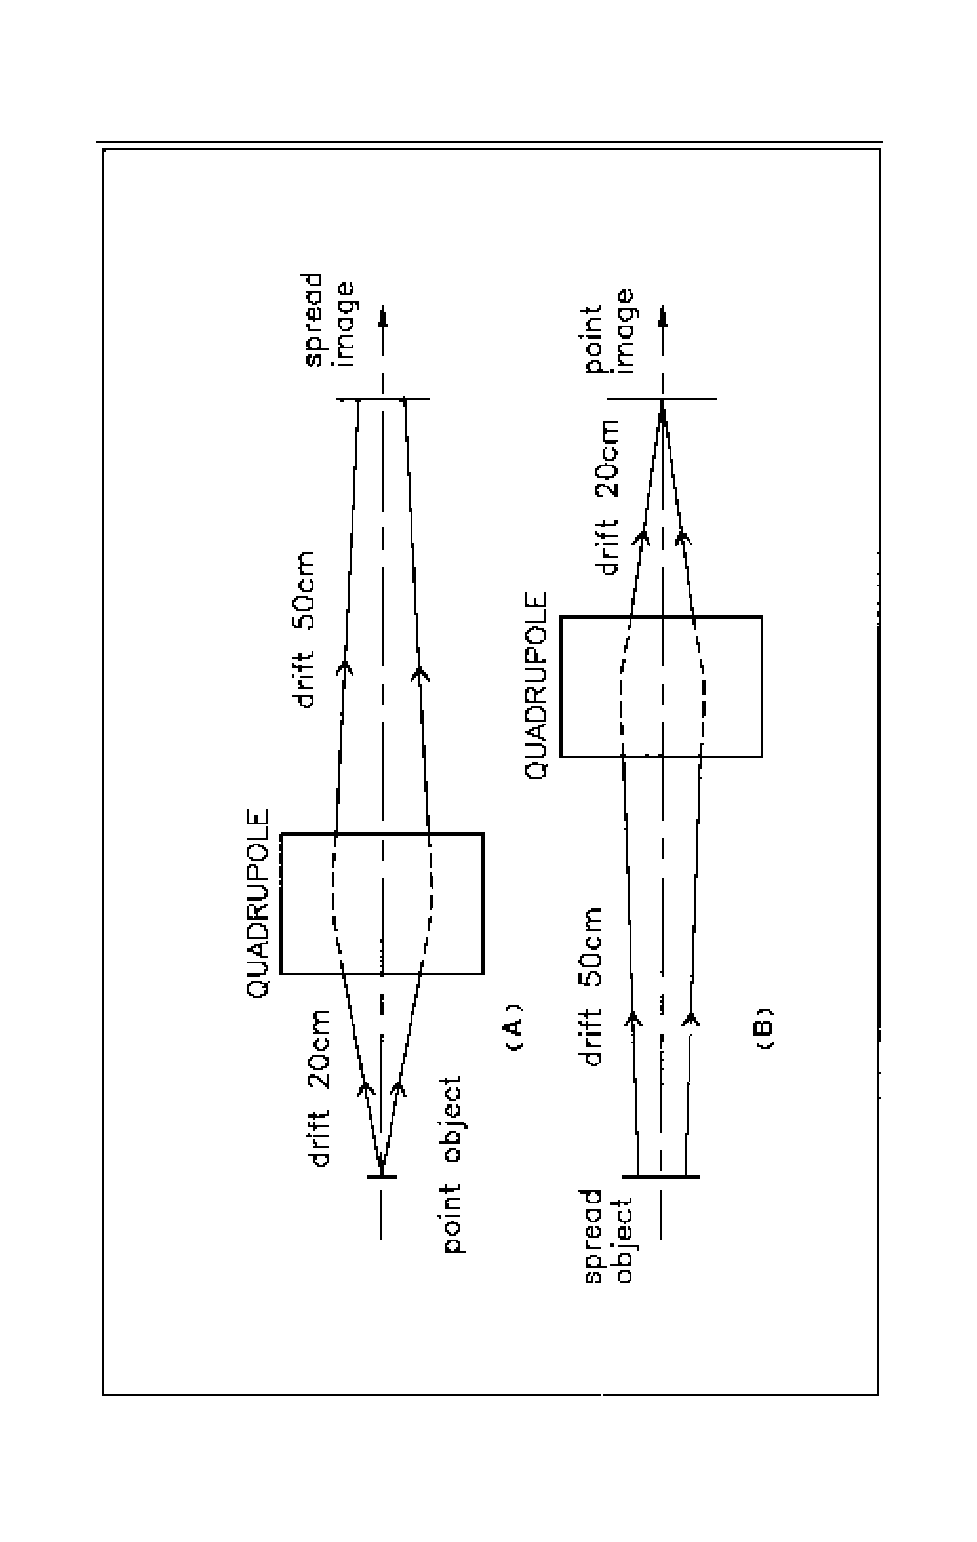
\includegraphics[height=12cm,angle=-90]{Fig36.ps}}
\hangcaption[Fig36]{\label{fig36}A. Regular forward ray-tracing, from object to image.\\
B. Same  structure, with backward ray-tracing from image to object~: negative integration step XPAS is used in  the quadrupole.}
\end{figure}


\subsubsection{Checking Fields and Trajectories Inside Optical Elements}  \label{sec4.6.1}
\index{checking field|textbf}\index{checking trajectories|textbf}

{\small $\bullet$} In all optical elements, an option $ \IL $\index{IL@{\IL}} is available.  It
is normally set to $\IL =0$ and in this case has no effect.

\noindent $ \IL=1 $ causes a print  in zgoubi.res \index{zgoubi.res} of particle 
coordinates and field
along trajectories in the optical element.  In the meantime, a calculation and summation of
the values of $ \vec  \nabla \cdot\vec  B$, 
 $ \vec  \nabla \times\vec  B $ and $ \nabla^2\vec  B $ (same for $\vec E$) at all 
integration steps is performed, which allows a check of the behavior of 
$ \vec  B $ (or $ \vec  E $) in field maps (all these derivatives should normally be zero).

\medskip

\noindent $ \IL=2 $ causes a print   of particle coordinates and other 
informations into the file  zgoubi.plt\index{zgoubi.plt} at each integration step~; this information 
 can further be processed with 
\textbf{zpop}\footnote{See Part D of the Guide.}\index{zpop}. In order to minimize  the volume of 
that storage file (when dealing with small step size, large number of particles, etc.) it is possible 
to print out  every other $10^n$ integration step by taking $ \IL=2 \times 10^n $ (for instance, 
 $ \IL=200 $ would cause output into zgoubi.plt every $100$ other step). 

\medskip

\noindent $ \IL=7 $ causes a print   of particle coordinates, fields, field derivatives  and other 
informations into the file  zgoubi.impdev.out\index{zgoubi.impdev.out|textbf}, 
one line of data  at each integration step. This information 
 can be further  plotted (\eg, using \zpop, or gnuplot). 
An example is given in fig.~\ref{figK1K2AGS}, a plot of the quadrupole and sextupole 
field indices along the reference orbit 
in a combined function main dipole pertaining to the AGS lattice~\cite{AGSModel}. 

%%%%%%%%%%%%%%figure%%%%%%%%%%%%%%
%\vspace{1cm}
\begin{figure}[h]
%\vspace{4.5 truecm}
%%%Figure 6
\centering
    \includegraphics*[width=.4\linewidth]{gnuplot_bderiv_DB.eps}
    \includegraphics*[width=.4\linewidth]{gnuplot_bderiv_DDB.eps}
{\setlength{\captionwidth}{0.7\linewidth}
\hangcaption[figK1K2AGS]{\label{figK1K2AGS} 
Typical field and derivatives, here, along the 10~GeV proton orbit across an AGS A-type main magnet. 
They are obtained from second degree polynomial interpolation from the magnet measured field map. 
Left~: $dB_Z(s)/dY$ and $dB_Y(s)/dZ$ , bottom~: $d^2B_Z(s)/dY^2$, $d^2B_Y(s)/dZdY$, $d^2B_Y(s)/dYdZ$.
These data were  stored in zgoubi.impdev.out\index{zgoubi.impdev.out} during execution, 
by stating $\IL=7$ under \textsl{TOSCA} keyword. 
}}
\end{figure}
%

\medskip

\noindent {\small $\bullet$} When dealing with field  maps (\emph{e.g.}, \textsl{CARTEMES\index{CARTEMES}}, \textsl{ELREVOL
\index{ELREVOL}, TOSCA\index{TOSCA}}), an option index $ \IC $\index{IC@{\IC}} is available.
  It is normally set to $\IC =0$ and in this case has no effect.
 
\noindent $ \IC=1 $ causes a print of the field map in zgoubi.res. \index{zgoubi.res}

\noindent $ \IC=2 $ will cause a print   of field maps into the file  zgoubi.map \index{zgoubi.map}
which can further be processed with \textbf{zpop} for plotting and other data treatment purposes. 
%%%%%%%\addtocounter{footnote}{-1}\footnotemark.


 \subsubsection{Labeling Keywords}\label{sec4.6.8}\index{LABEL@{\LABEL}|textbf}

Keywords in \zgou\ input data file zgoubi.dat can be \LABEL'ed, for the purpose of 
the execution of such procedures as  \textsl{REBELOTE, \index{REBELOTE} PICKUPS}\index{PICKUPS}, 
\textsl{FAISCNL}, \textsl{FAISTORE}, 
\index{FAISCNL}\index{FAISTORE} \textsl{SCALING},\index{SCALING} and also for the purpose of 
particle coordinate storage into zgoubi.plt\index{zgoubi.plt} (see section~\ref{sec4.6.1}, 
$\IL=2$ option). 

\medskip 

\noindent A keyword in zgoubi.dat accepts two \LABEL's. The first one is used for the 
above mentioned purposes, the second one (set to ``.plt'' in that case) is used essentially 
 with \textsl{MARKER} for storage of current particle data 
into zgoubi.plt. The keyword and its \LABEL['s] should fit within a 110-character 
long string on a single line (a quantity set in the \FORTRAN\ file \texttt{prdata.f}). 

\subsubsection{Multi-turn Tracking in Circular Machines \label{sec4.6.5} } \index{multi-turn tracking|textbf}

Multi-turn tracking  in circular machines can be performed by
means of the keyword \textsl{REBELOTE\index{REBELOTE}}. \textsl{REBELOTE} is introduced in 
the  zgoubi.dat data list with its argument \textsl{NPASS}$+1$\index{NPASS} being the number of turns to be 
performed. 
It will cause a jump of  the ``multi-turn pointer''  back to (details on page~\pageref{REBELOTE}), 
either the beginning of the data list (default case), or to a particular \textsl{LABEL} 
in that list. From then on, tracking resumes down to \textsl{REBELOTE} again, and so forth until the 
requested number of passes has been reached. 

\medskip

\noindent Possible magnet  timing laws $ B(T)$  during the multi-turn process 
(with $T=1 $ to \textsl{NPASS}$+1$  counted in number of turns) can be introduced by means of \textsl{SCALING}. 

\medskip 

\noindent In order that the \IMAX\index{IMAX@{\IMAX}} particles of the beam start a new 
pass with the coordinates they had reached at the end of the 
previous one, the option $ K=99 $ has to be specified in \textsl{REBELOTE\index{REBELOTE}}.

\medskip


\noindent\textbf{Synchrotron acceleration} can be simulated, using following the procedure~: 
\begin{itemize}
\item[-] \textsl{CAVITE\index{CAVITE}} appears in the zgoubi.dat data list (normally before
\textsl{REBELOTE\index{REBELOTE}}), with option \textsl{IOPT}$\neq 0$, 

\item[-] the RF frequency of the cavity may be given a timing law $f_{RF}(T)$ by 
means of \textsl{SCALING\index{SCALING}}, family \textsl{CAVITE}, 

\item[-] the magnets are given a field  timing law $ B(T)$,  
(with $T=1 $ to \textsl{NPASS}$+1$  counted in number of turns) by means of \textsl{SCALING}. \par
\end{itemize}

\noindent Eventually some families of magnets may be given a different timing law 
    for the simulation of special processes (\emph{e.g.}, time varying orbit bump, 
fast crossing of spin resonances with families of jump quadrupoles). 

%\noindent This is illustrated in the example~6 of Part~C.  %%%% ref




\subsubsection{Positioning, (Mis-)Alignment, of Optical Elements and Field Maps} \label{sec4.6.2} 
\index{positioning of optical elements|textbf} \index{alignment (mis-) of optical elements|textbf} \index{misalignment|textbf}

The last record in most optical elements and field maps is the positioning option 
\textsl{KPOS}\index{KPOS|textbf}. \KPOS\ is followed by the positioning parameters, 
\eg, \textsl{XCE}, \textsl{YCE} 
for translation and \textsl{ALE} for rotation. The positioning works in two different ways, 
depending  whether the element is  defined in 
Cartesian $ (X, Y, Z) $ coordinates (\emph{e.g.}, \textsl{QUADRUPO\index{QUADRUPO}, TOSCA\index{TOSCA}}),
 or polar 
 ($R$, $\theta$, $Z$)  coordinates (\textsl{DIPOLE\index{DIPOLE}}). 
 
 \subsubsection*{Cartesian Coordinates~: }   \index{cartesian coordinates|textbf} 
 
 If \textsl{KPOS} $ =1$, the optical element is moved (shifted by \textsl{XCE, YCE} and Z-rotated by 
\textsl{ALE}) with respect to the incoming reference frame. Trajectory coordinates after traversal of the 
element refer the element frame. 

\medskip

\noindent If  \KPOS$=2 $, the shifts  \XCE\index{XCE@\XCE}   
and   \YCE\index{YCE@\YCE}, and the tilt angle \ALE\index{\ALE@{\textsl{ALE}}}   are taken into 
account, for mis-aligning  the element with respect to the incoming 
reference, as shown in Fig.~\ref{fig34}.  
The effect is equivalent to  a \textsl{CHANGREF(\XCE,\YCE,\ALE)}  upstream of the 
optical element, followed by   \textsl{CHANGREF($\XCS$,$\YCS$,$\ALS=-\ALE$)} downstream of it, with 
 computed \XCS, \YCS\ values as schemed in Fig.~\ref{fig34}.  

\medskip

\noindent \textsl{KPOS} $=3 $ option is available for a limited number of  
 magnets  (\emph{e.g.}, \textsl{BEND}, \textsl{MULTIPOL}, \textsl{AGSMM} \index{AGSMM})~; 
it is effective only if a non zero dipole component $B1$ is present, or if  \textsl{ALE} is non-zero. 
It positions automatically the magnet in a symmetric manner with respect to the incoming and outgoing reference 
axis, convenient for periodic structures, as follows (Fig~\ref{figKPOS3}). 

\medskip
 
\noindent Both incoming and outgoing reference frames are  tilted w.r.t. the magnet,  

 $\bullet$ either,  by an angle \textsl{ALE}  if ALE$\not =$0, 

 $\bullet$ or, if ALE=0  by  half the \textsl{Z}-rotation $\theta_Z/2$ such that $ L = 
2 \dfrac{\BORO}{B1} \sin({\theta_Z}/{2})$,  wherein $L$ = geometrical length, 
\BORO\  = reference rigidity as defined in \textsl{OBJET\index{OBJET}}.
%\noindent This is equivalent to the sequence \textsl{CHANGREF(0,0,-$\theta$/2)},
%  \textsl{CHANGREF(0,YCE,0)} right upstream the magnet, followed  by 
%\textsl{CHANGREF(0,-YCE,-$\theta$/2)}.

\noindent Next, the optical element is  Y-shifted by \textsl{YCE} (\textsl{XCE} is not used) in a 
direction orthogonal to the new magnet axis (\emph{i.e.}, at an angle $ALE+\pi/2$ \wrt\ the $X$ axis of the incoming 
reference frame).


%%%%%%%%%%%%%%figure%%%%%%%%%%%%%%

\begin{figure}[h]
\begin{center}
%\begin{minipage}{.45\linewidth}
%\begin{center}

\mbox{
\includegraphics[height=4cm]{Fig34A.eps} \hspace{.02\linewidth}
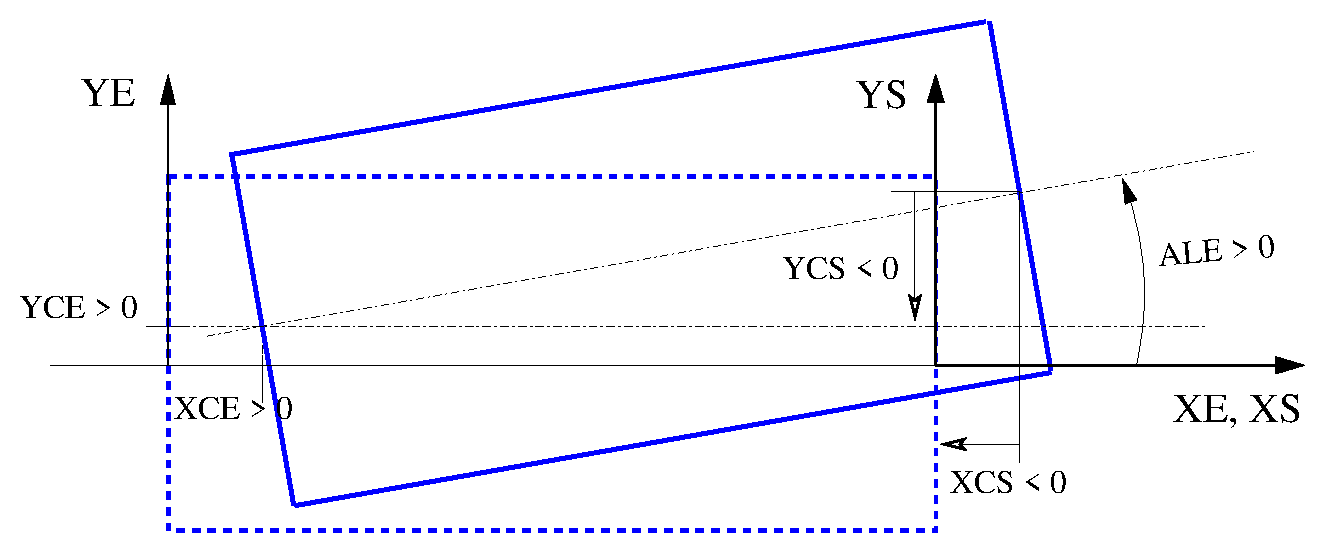
\includegraphics[height=3.7cm]{Fig34.eps}
}
{\setlength{\captionwidth}{16cm}
\hangcaption{\label{fig34} 
Case of Cartesian frame optical element. 
  Left~: moving an optical element using  \textsl{KPOS}$=1 $. 
Right~: Mis-aligning  an optical element using  \textsl{KPOS}$=2 $.  
\textsl{$(X_E,Y_E)$} and \textsl{$(X_S, Y_S)$} are respectively the incoming 
 and outgoing  reference frames.
}}
%\end{center}
%\end{minipage}  %\hspace{.05\linewidth}
%\begin{minipage}{.45\linewidth}
%\begin{center}
\end{center}
\end{figure}


\begin{figure}[h]
\begin{center}
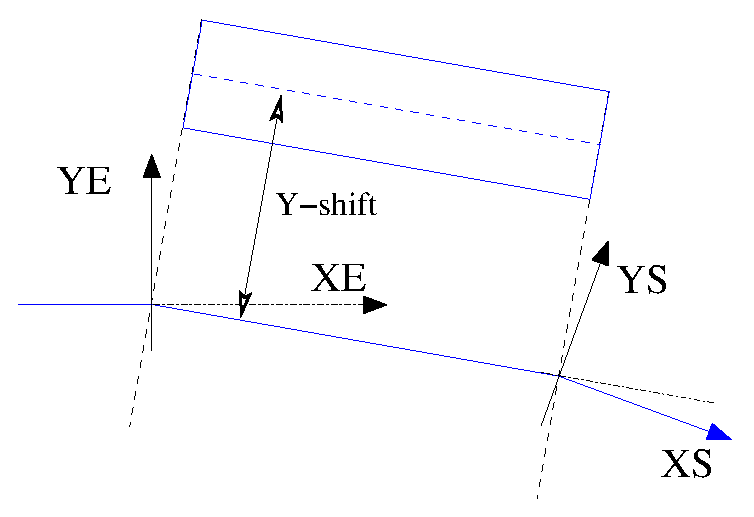
\includegraphics[height=5cm]{FigKPOS3.eps}

\hangcaption{\label{figKPOS3} 
Case of Cartesian frame optical element. 
Alignment of a  bend by half the deviation, using  \textsl{KPOS}$=3 $.  
\textsl{$(X_E,Y_E)$} and \textsl{$(X_S, Y_S)$} are respectively the incoming 
 and outgoing  reference frames.
}
%\end{center}
%\end{minipage}
%\end{center}
%\end{figure}
%%%%%%%%%%%%%%figure%%%%%%%%%%%%%%
%\begin{figure}
%\vspace{12 truecm}
%%%Figure 35
\end{center}
\end{figure}

\noindent \textsl{KPOS} $=4 $ applies to a limited number of optical elements, as 
\textsl{AGSMM} (AGS main magnet). \index{AGSMM} 
By default, it aligns the magnet in a way similar 
to  \textsl{KPOS} $=3 $, with reference frame Z-rotated by $\theta_Z/2$ as drawn from $ L = 
2 \dfrac{\BORO}{B1} \sin({\theta_Z}/{2})$. However magnet mis-alignment (alignment errors) are handled in a 
specific way, as follows. 



\begin{figure}[h]

\noindent All 6 types of misalignments, namely, X-, Y-, Z-shift, X-, Y-, Z-rotation, can be accounted for, in an arbitrary order. 
They are specified using the ``new style'' \textsl{CHANGREF} method as described in page~\pageref{CHANGREFNew}. 
Longitudinal rotation ``XR'' is taken \wrt\ the longitudinal axis, whereas radial and axial rotations, ``YR'' and ``ZR'', 
 are  with respect to an axis going through the center of the magnet. 
% Transformations are as follows, see Fig.~\ref{figPitch}~: 

%\medskip
%
%\noindent {\small $\bullet$} Y-rotation (pitch) by an angle $\varphi$~:  new coordinates (at $M$) as well as path 
%lengthening, etc, derive  from old ones (at $M_0$) following\\
%$X_{new} = 0$ by definition, \\
%$Y_{new} = Y_{old} + dS \cos P \sin T$, $dS$ is the path lengthening, given below, \\
%$Z_{new} = Z_{old} \cos p/\cos (p-\varphi)$, ensuing from $\varphi = \dfrac{\pi}{2} - p $, and $\tan p = \tan P / \cos T$ (since
%$om\, \cos p= OM\cos P \cos T $ as well as $om\, \sin p= OM \sin P$), \\
%$dS = dL/\cos P / \cos T$ with $d L = sign(dL, -Z_{new} \varphi) \sqrt{Z_{new}^2 \sin^2 \varphi+(Z_{new} \cos \varphi -Z_{old})^2}$. 
%
%\noindent {\small $\bullet$} etc.

\vspace{5ex}

\begin{center}
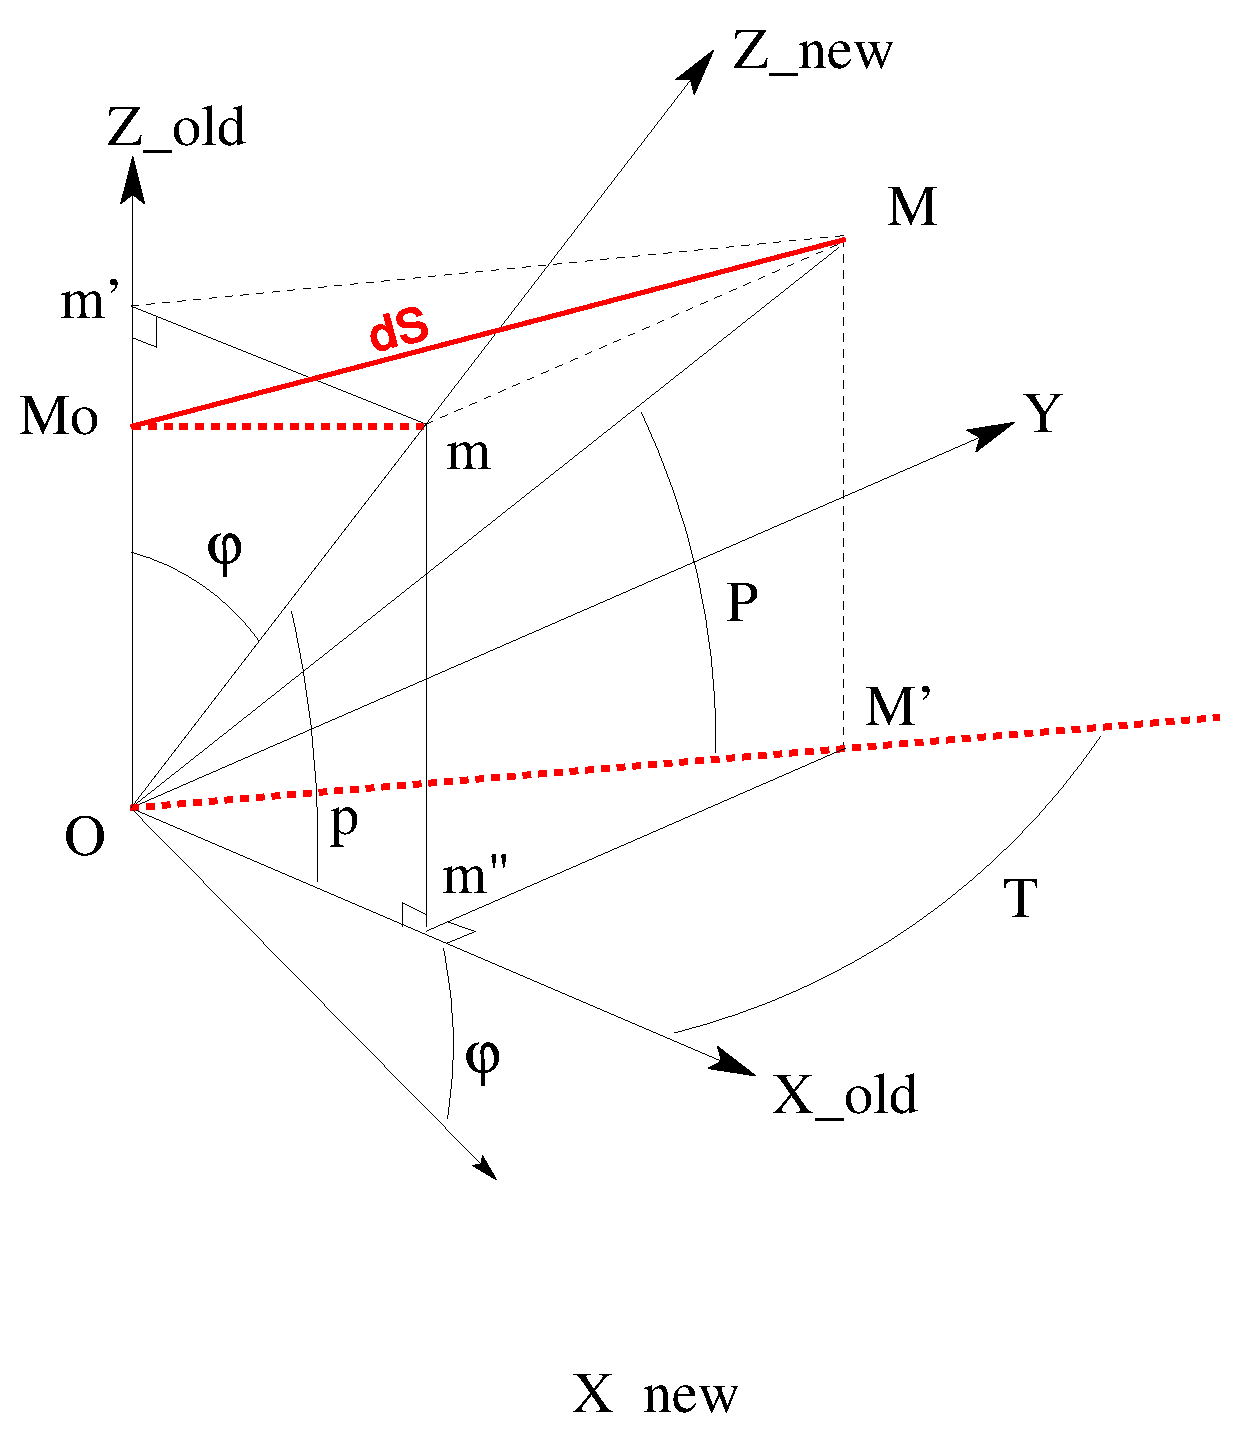
\includegraphics[height=9cm]{FigPitch.eps}
\hangcaption{\label{figPitch}Pitch angle, $\varphi$, in the``YR'' type of rotation, using \textsl{KPOS}$=4 $. 
$M$ is the new position, in the rotated plane $(Y,Z_{new})$, of a particle with velocity $\vec v // \vec{M_oM}$ located  
at former position $M_o$ in the old, $(Y,Z_{old})$, plane. $M'$, $m$, $m'$ are projections of $M$, $m''$ is projection of $M'$. 
$T$ and $P$ are the  horizontal and vertical angles as defined in Fig.~\ref{fig1}. 
$p$ is the projection of $P$. 
}
%\end{center}
%\end{figure}
%
%\begin{figure}[h]
%\begin{center}

\vspace{10ex}

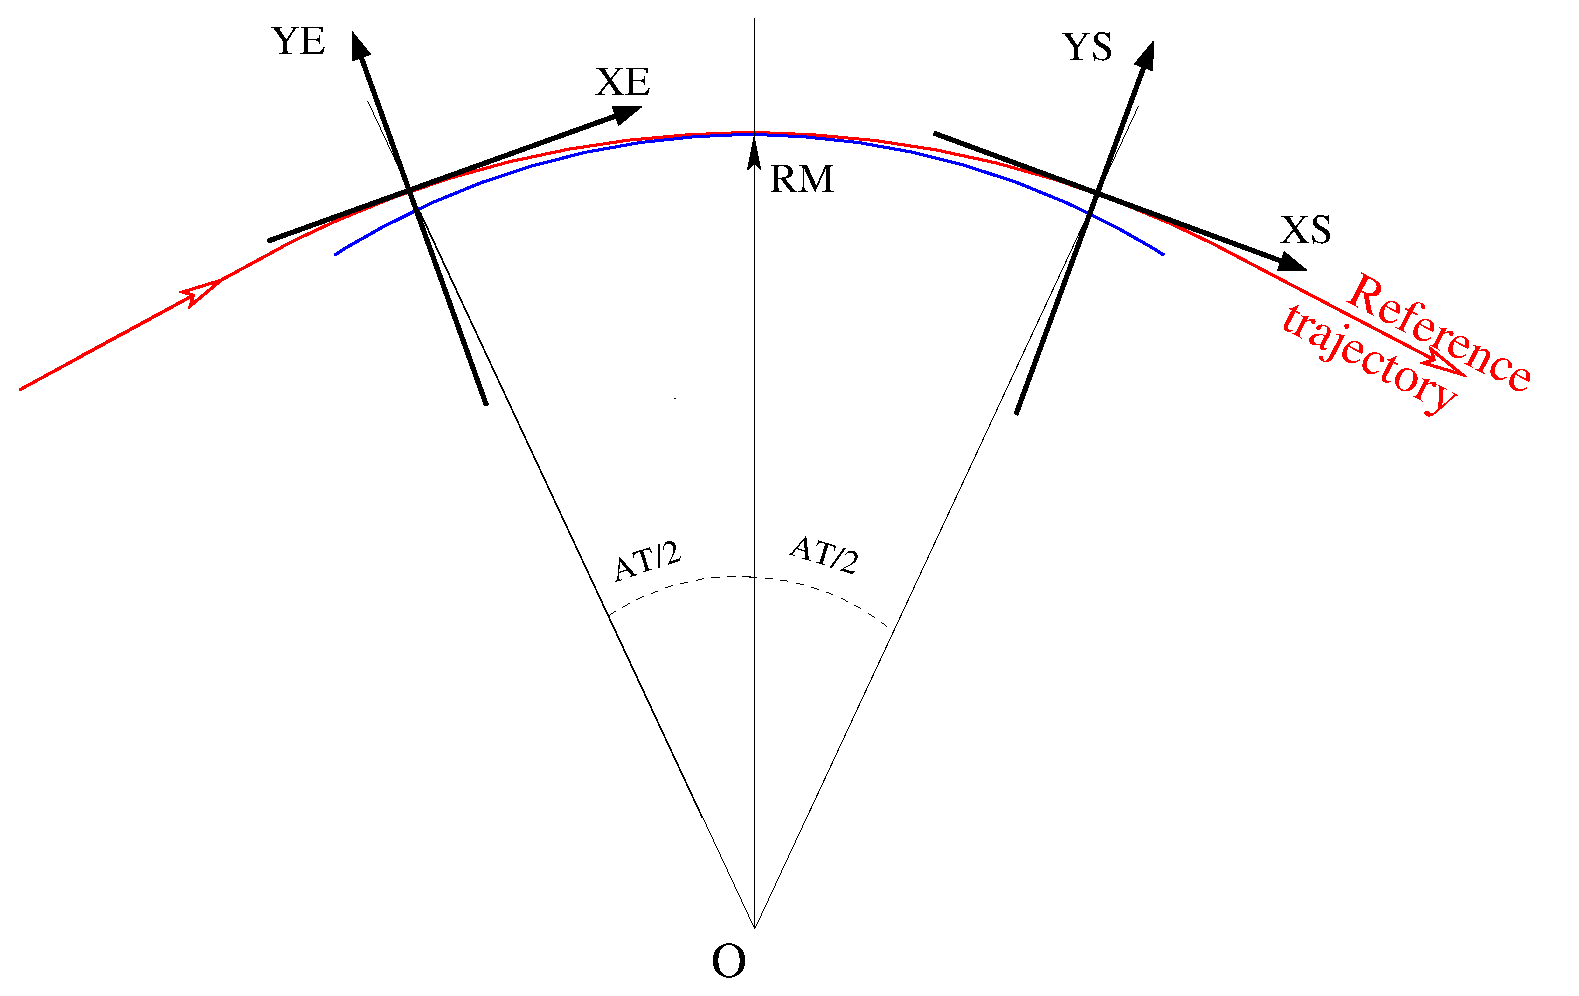
\includegraphics[height=6cm]{Fig35.eps}
\hangcaption{\label{fig35}Positioning of a polar field map, using \textsl{KPOS}$=1 $.}
\end{center}

\vfill
\end{figure}


\medskip





\clearpage 

 \subsubsection*{Polar Coordinates}   \index{polar coordinates|textbf} 
 
 If  \textsl{KPOS} $=1$,  the element is positioned automatically in such a way
that a particle entering with zero initial coordinates and 
$ 1+DP=\Br /\BORO $ 
relative rigidity will reach position ($ RM$, $\dfrac{AT }{ 2} $) in 
the element with $ T=0 $ angle with respect to the moving frame in the polar 
coordinates system of the element (Fig.~\ref{fig35}~; 
see \textsl{DIPOLE-M\index{DIPOLE-M}} and \textsl{POLARMES\index{POLARMES}}).

\noindent If  \textsl{KPOS} $=2, $ the map is positioned in such a way that the 
incoming reference frame is presented  at radius $ RE $ with angle $ TE $.  
The exit reference frame  is positioned in a similar way with 
respect to the map,  by means of 
the two parameters $ RS $ (radius) and $ TS $ (angle) (see Fig.~\ref{fig9}A page~\pageref{fig9}A).  






 \subsubsection{Coded Integration Step\index{XPAS, coded}\index{integration step size!coded|textbf}} 

In several optical elements (\emph{e.g.}, all multipoles, \textsl{BEND}) the 
integration step (in general noted \textsl{XPAS}) can be coded under the 
form \textsl{XPAS} = \texttt{\#E|C|S}, with \texttt{E}, \texttt{C}, \texttt{S} integers, \texttt{E} is the number of
steps  in the entrance fringe field region, \texttt{C} is the number of
steps in the magnet body, and \texttt{S} is the number of steps in the 
exit fringe field region.

\subsubsection{Ray-tracing of an Arbitrarily Large Number of Particles} \index{multi-particle|textbf} \index{Monte Carlo}
  \label{sec4.6.4}

Monte Carlo  multi-particle simulations involving an 
arbitrarily large number of particles
can be performed using  \textsl{MCOBJET} together with \textsl{REBELOTE\index{REBELOTE}}, put at the end of the optical
structure, with its argument \textsl{NPASS}\index{NPASS} being the number of passes through 
\textsl{REBELOTE\index{REBELOTE}}, and (\textsl{NPASS}$+ 1$) * \IMAX\index{IMAX@{\IMAX}}  
the number of particles to 
be ray-traced. In order that new initial conditions  ($D$, $Y$, $T$, $Z$, 
$P$, $X$) 
 be generated at each pass, $ K=0 $ has to be specified in \textsl{REBELOTE\index{REBELOTE}}.
 
\noindent Statistics on coordinates, spins\index{spin tracking}, and other histograms can be
performed by means of such procedures as \textsl{HISTO\index{HISTO}, SPNTRK\index{SPNTRK}}, 
etc. that stack the information from pass to pass. 


\subsubsection{Stopped Particles~: The \IEX\ Flag} 
\label{sec4.6.6}\index{stopped particles|textbf}\index{IEX@{\IEX}|textbf}

As described in \textsl{OBJET\index{OBJET}}, each particle $I=1$, \IMAX\
 is attached a
value $\IEX(I)$ of the \IEX\ flag. Normally, $\IEX(I)=1$. Under certain 
circumstances, \IEX\ may be changed to a negative value by \zgoubi, as follows. 

\begin{itemize}
\item[$-1$]~:  the trajectory happened to wander outside the limits of a field map 
\item[$-2$]~:  too many integration steps\index{integration step size} in an optical element (a quantity controlled in 
\texttt{MXSTEP.H} include file)
\item[$-3$]~:  deviation happened to exceed $\pi / 2 $ in an optical element not designed to allow that
\item[$-4$]~:  stopped by walls (procedures \textsl{CHAMBR, COLLIMA})  
\item[$-5$]~:  too many iterations in subroutine \texttt{depla.f}  
\item[$-6$]~:  energy loss exceeds particle energy 
\item[$-7$]~:  field discontinuities larger than 50\% within a field map
\item[$-8$]~:  reached field limit in an optical element
\end{itemize}


\noindent Only in the case $\IEX=-1$ will the integration not be stopped since in this case 
the field outside the map is extrapolated from the map data, and the particle may possibly get 
back into the map (see section~\ref{sec2.4.2} on page~\pageref{sec2.4.2}).  In all other cases 
  the particle will be stopped. 

\subsubsection{Negative Rigidity} \label{sec4.6.7}  \index{negative rigidity|textbf} 
\index{negative charge}\index{negative momentum}

\zgou\ can handle negative rigidities $\Br = p/q$. This is equivalent to 
considering either particles with negative charge ($q<0$) or
momentum ($p<0$), or  reversed fields (\wrt~the field sign 
that shows in the zgoubi.dat optical element data list).

\noindent Negative rigidities may be specified in terms of 
$\BORO <0$ or $D=\Br / \BORO < 0$ when 
defining the initial coordinates with \textsl{OBJET}\index{OBJET} or \textsl{MCOBJET}\index{MCOBJET}.
